\documentclass[twoside]{book}

% Packages required by doxygen
\usepackage{fixltx2e}
\usepackage{calc}
\usepackage{doxygen}
\usepackage{graphicx}
\usepackage[utf8]{inputenc}
\usepackage{makeidx}
\usepackage{multicol}
\usepackage{multirow}
\PassOptionsToPackage{warn}{textcomp}
\usepackage{textcomp}
\usepackage[nointegrals]{wasysym}
\usepackage[table]{xcolor}

% Font selection
\usepackage[T1]{fontenc}
\usepackage{mathptmx}
\usepackage[scaled=.90]{helvet}
\usepackage{courier}
\usepackage{amssymb}
\usepackage{sectsty}
\renewcommand{\familydefault}{\sfdefault}
\allsectionsfont{%
  \fontseries{bc}\selectfont%
  \color{darkgray}%
}
\renewcommand{\DoxyLabelFont}{%
  \fontseries{bc}\selectfont%
  \color{darkgray}%
}
\newcommand{\+}{\discretionary{\mbox{\scriptsize$\hookleftarrow$}}{}{}}

% Page & text layout
\usepackage{geometry}
\geometry{%
  a4paper,%
  top=2.5cm,%
  bottom=2.5cm,%
  left=2.5cm,%
  right=2.5cm%
}
\tolerance=750
\hfuzz=15pt
\hbadness=750
\setlength{\emergencystretch}{15pt}
\setlength{\parindent}{0cm}
\setlength{\parskip}{0.2cm}
\makeatletter
\renewcommand{\paragraph}{%
  \@startsection{paragraph}{4}{0ex}{-1.0ex}{1.0ex}{%
    \normalfont\normalsize\bfseries\SS@parafont%
  }%
}
\renewcommand{\subparagraph}{%
  \@startsection{subparagraph}{5}{0ex}{-1.0ex}{1.0ex}{%
    \normalfont\normalsize\bfseries\SS@subparafont%
  }%
}
\makeatother

% Headers & footers
\usepackage{fancyhdr}
\pagestyle{fancyplain}
\fancyhead[LE]{\fancyplain{}{\bfseries\thepage}}
\fancyhead[CE]{\fancyplain{}{}}
\fancyhead[RE]{\fancyplain{}{\bfseries\leftmark}}
\fancyhead[LO]{\fancyplain{}{\bfseries\rightmark}}
\fancyhead[CO]{\fancyplain{}{}}
\fancyhead[RO]{\fancyplain{}{\bfseries\thepage}}
\fancyfoot[LE]{\fancyplain{}{}}
\fancyfoot[CE]{\fancyplain{}{}}
\fancyfoot[RE]{\fancyplain{}{\bfseries\scriptsize Generated on Sun Oct 16 2016 23\+:13\+:34 for C++ Web Framework by Doxygen }}
\fancyfoot[LO]{\fancyplain{}{\bfseries\scriptsize Generated on Sun Oct 16 2016 23\+:13\+:34 for C++ Web Framework by Doxygen }}
\fancyfoot[CO]{\fancyplain{}{}}
\fancyfoot[RO]{\fancyplain{}{}}
\renewcommand{\footrulewidth}{0.4pt}
\renewcommand{\chaptermark}[1]{%
  \markboth{#1}{}%
}
\renewcommand{\sectionmark}[1]{%
  \markright{\thesection\ #1}%
}

% Indices & bibliography
\usepackage{natbib}
\usepackage[titles]{tocloft}
\setcounter{tocdepth}{3}
\setcounter{secnumdepth}{5}
\makeindex

% Hyperlinks (required, but should be loaded last)
\usepackage{ifpdf}
\ifpdf
  \usepackage[pdftex,pagebackref=true]{hyperref}
\else
  \usepackage[ps2pdf,pagebackref=true]{hyperref}
\fi
\hypersetup{%
  colorlinks=true,%
  linkcolor=blue,%
  citecolor=blue,%
  unicode%
}

% Custom commands
\newcommand{\clearemptydoublepage}{%
  \newpage{\pagestyle{empty}\cleardoublepage}%
}


%===== C O N T E N T S =====

\begin{document}

% Titlepage & ToC
\hypersetup{pageanchor=false,
             bookmarks=true,
             bookmarksnumbered=true,
             pdfencoding=unicode
            }
\pagenumbering{roman}
\begin{titlepage}
\vspace*{7cm}
\begin{center}%
{\Large C++ Web Framework }\\
\vspace*{1cm}
{\large Generated by Doxygen 1.8.8}\\
\vspace*{0.5cm}
{\small Sun Oct 16 2016 23:13:34}\\
\end{center}
\end{titlepage}
\clearemptydoublepage
\tableofcontents
\clearemptydoublepage
\pagenumbering{arabic}
\hypersetup{pageanchor=true}

%--- Begin generated contents ---
\chapter{Namespace Index}
\section{Namespace List}
Here is a list of all namespaces with brief descriptions\+:\begin{DoxyCompactList}
\item\contentsline{section}{\hyperlink{namespace_c_w_f}{C\+W\+F} \\*All classes of C++ Web Framework are contained within the namespace \hyperlink{namespace_c_w_f}{C\+W\+F} }{\pageref{namespace_c_w_f}}{}
\end{DoxyCompactList}

\chapter{Hierarchical Index}
\section{Class Hierarchy}
This inheritance list is sorted roughly, but not completely, alphabetically\+:\begin{DoxyCompactList}
\item \contentsline{section}{C\+W\+F\+:\+:Configuration}{\pageref{class_c_w_f_1_1_configuration}}{}
\item \contentsline{section}{C\+W\+F\+:\+:Cpp\+Web\+Application}{\pageref{class_c_w_f_1_1_cpp_web_application}}{}
\item \contentsline{section}{C\+W\+F\+:\+:C\+S\+T\+L\+Compiler}{\pageref{class_c_w_f_1_1_c_s_t_l_compiler}}{}
\item \contentsline{section}{C\+W\+F\+:\+:C\+S\+T\+L\+Compiler\+Attributes}{\pageref{class_c_w_f_1_1_c_s_t_l_compiler_attributes}}{}
\item \contentsline{section}{C\+W\+F\+:\+:C\+S\+T\+L\+Compiler\+For}{\pageref{class_c_w_f_1_1_c_s_t_l_compiler_for}}{}
\item \contentsline{section}{C\+W\+F\+:\+:C\+S\+T\+L\+Compiler\+If}{\pageref{class_c_w_f_1_1_c_s_t_l_compiler_if}}{}
\item \contentsline{section}{C\+W\+F\+:\+:File\+Manager}{\pageref{class_c_w_f_1_1_file_manager}}{}
\item \contentsline{section}{C\+W\+F\+:\+:Filter}{\pageref{class_c_w_f_1_1_filter}}{}
\item \contentsline{section}{C\+W\+F\+:\+:Filter\+Chain}{\pageref{class_c_w_f_1_1_filter_chain}}{}
\item \contentsline{section}{C\+W\+F\+:\+:For\+Attributes}{\pageref{class_c_w_f_1_1_for_attributes}}{}
\item \contentsline{section}{C\+W\+F\+:\+:Http\+Cookie}{\pageref{class_c_w_f_1_1_http_cookie}}{}
\item \contentsline{section}{C\+W\+F\+:\+:Http\+Parser}{\pageref{class_c_w_f_1_1_http_parser}}{}
\item \contentsline{section}{C\+W\+F\+:\+:Http\+Request\+Method}{\pageref{class_c_w_f_1_1_http_request_method}}{}
\item \contentsline{section}{C\+W\+F\+:\+:Http\+Servlet}{\pageref{class_c_w_f_1_1_http_servlet}}{}
\begin{DoxyCompactList}
\item \contentsline{section}{C\+W\+F\+:\+:Cpp\+Web\+Servlet}{\pageref{class_c_w_f_1_1_cpp_web_servlet}}{}
\end{DoxyCompactList}
\item \contentsline{section}{C\+W\+F\+:\+:Http\+Servlet\+Response}{\pageref{class_c_w_f_1_1_http_servlet_response}}{}
\item \contentsline{section}{C\+W\+F\+:\+:Http\+Session}{\pageref{class_c_w_f_1_1_http_session}}{}
\item \contentsline{section}{C\+W\+F\+:\+:If\+Attributes}{\pageref{class_c_w_f_1_1_if_attributes}}{}
\item \contentsline{section}{C\+W\+F\+:\+:Meta\+Class\+Parser}{\pageref{class_c_w_f_1_1_meta_class_parser}}{}
\item \contentsline{section}{C\+W\+F\+:\+:Properties}{\pageref{class_c_w_f_1_1_properties}}{}
\item \contentsline{section}{C\+W\+F\+:\+:Q\+Map\+Thread\+Safety$<$ Key, T $>$}{\pageref{class_c_w_f_1_1_q_map_thread_safety}}{}
\item \contentsline{section}{C\+W\+F\+:\+:Q\+Map\+Thread\+Safety$<$ Q\+String, C\+W\+F\+:\+:Http\+Servlet $\ast$ $>$}{\pageref{class_c_w_f_1_1_q_map_thread_safety}}{}
\item \contentsline{section}{C\+W\+F\+:\+:Q\+Map\+Thread\+Safety$<$ Q\+String, C\+W\+F\+:\+:Http\+Session $\ast$ $>$}{\pageref{class_c_w_f_1_1_q_map_thread_safety}}{}
\item \contentsline{section}{C\+W\+F\+:\+:Q\+Map\+Thread\+Safety$<$ Q\+String, Q\+Object $\ast$ $>$}{\pageref{class_c_w_f_1_1_q_map_thread_safety}}{}
\item Q\+Object\begin{DoxyCompactList}
\item \contentsline{section}{C\+W\+F\+:\+:C\+S\+T\+L\+Compiler\+Object}{\pageref{class_c_w_f_1_1_c_s_t_l_compiler_object}}{}
\item \contentsline{section}{C\+W\+F\+:\+:Http\+Servlet\+Request}{\pageref{class_c_w_f_1_1_http_servlet_request}}{}
\item \contentsline{section}{C\+W\+F\+:\+:Q\+List\+Object}{\pageref{class_c_w_f_1_1_q_list_object}}{}
\end{DoxyCompactList}
\item Q\+Runnable\begin{DoxyCompactList}
\item \contentsline{section}{C\+W\+F\+:\+:Http\+Read\+Request}{\pageref{class_c_w_f_1_1_http_read_request}}{}
\end{DoxyCompactList}
\item Q\+Tcp\+Server\begin{DoxyCompactList}
\item \contentsline{section}{C\+W\+F\+:\+:Cpp\+Web\+Server}{\pageref{class_c_w_f_1_1_cpp_web_server}}{}
\end{DoxyCompactList}
\item \contentsline{section}{C\+W\+F\+:\+:Request\+Dispatcher}{\pageref{class_c_w_f_1_1_request_dispatcher}}{}
\item \contentsline{section}{C\+W\+F\+:\+:Session\+Id\+Generator}{\pageref{class_c_w_f_1_1_session_id_generator}}{}
\end{DoxyCompactList}

\chapter{Class Index}
\section{Class List}
Here are the classes, structs, unions and interfaces with brief descriptions\+:\begin{DoxyCompactList}
\item\contentsline{section}{\hyperlink{class_c_w_f_1_1_configuration}{C\+W\+F\+::\+Configuration} \\*This class is responsable to read a ini file and extract its information }{\pageref{class_c_w_f_1_1_configuration}}{}
\item\contentsline{section}{\hyperlink{class_c_w_f_1_1_cpp_web_application}{C\+W\+F\+::\+Cpp\+Web\+Application} \\*This class is responsible for encapsulating the Q\+Core\+Application, the \hyperlink{class_c_w_f_1_1_cpp_web_server}{Cpp\+Web\+Server} and configure the server logging mechanism }{\pageref{class_c_w_f_1_1_cpp_web_application}}{}
\item\contentsline{section}{\hyperlink{class_c_w_f_1_1_cpp_web_server}{C\+W\+F\+::\+Cpp\+Web\+Server} \\*H\+T\+T\+P server, responsable to receive and dispatch the requisitions }{\pageref{class_c_w_f_1_1_cpp_web_server}}{}
\item\contentsline{section}{\hyperlink{class_c_w_f_1_1_cpp_web_servlet}{C\+W\+F\+::\+Cpp\+Web\+Servlet} \\*This class is responsible for displaying the standard pages of C++ Web Framework\+: index, examples, documentation, ssl and authors }{\pageref{class_c_w_f_1_1_cpp_web_servlet}}{}
\item\contentsline{section}{\hyperlink{class_c_w_f_1_1_c_s_t_l_compiler}{C\+W\+F\+::\+C\+S\+T\+L\+Compiler} \\*This class compiles xhtml pages with C\+S\+T\+L (C++ Server Pages Standard Tags Library) }{\pageref{class_c_w_f_1_1_c_s_t_l_compiler}}{}
\item\contentsline{section}{\hyperlink{class_c_w_f_1_1_c_s_t_l_compiler_attributes}{C\+W\+F\+::\+C\+S\+T\+L\+Compiler\+Attributes} \\*This class search for expressions \#\{obj.\+get\} and compiles it }{\pageref{class_c_w_f_1_1_c_s_t_l_compiler_attributes}}{}
\item\contentsline{section}{\hyperlink{class_c_w_f_1_1_c_s_t_l_compiler_for}{C\+W\+F\+::\+C\+S\+T\+L\+Compiler\+For} \\*Extracts and valites all attibutes from a \char`\"{}for\char`\"{} tag }{\pageref{class_c_w_f_1_1_c_s_t_l_compiler_for}}{}
\item\contentsline{section}{\hyperlink{class_c_w_f_1_1_c_s_t_l_compiler_if}{C\+W\+F\+::\+C\+S\+T\+L\+Compiler\+If} \\*Extracts and valites all attibutes from a \char`\"{}if\char`\"{} tag }{\pageref{class_c_w_f_1_1_c_s_t_l_compiler_if}}{}
\item\contentsline{section}{\hyperlink{class_c_w_f_1_1_c_s_t_l_compiler_object}{C\+W\+F\+::\+C\+S\+T\+L\+Compiler\+Object} \\*The \hyperlink{class_c_w_f_1_1_properties}{Properties} class is an auxiliar class to the \hyperlink{class_c_w_f_1_1_c_s_t_l_compiler}{C\+S\+T\+L\+Compiler} }{\pageref{class_c_w_f_1_1_c_s_t_l_compiler_object}}{}
\item\contentsline{section}{\hyperlink{class_c_w_f_1_1_file_manager}{C\+W\+F\+::\+File\+Manager} \\*Can manage file's name }{\pageref{class_c_w_f_1_1_file_manager}}{}
\item\contentsline{section}{\hyperlink{class_c_w_f_1_1_filter}{C\+W\+F\+::\+Filter} \\*Works like a filter. You can use this class to validate sessions or measuring runtime of a specific method, for example. To use this class, you will need to create a derived class and reconstruct the do\+Filter method, after this, you will need to configure it into the Configure\+Cpp\+Web\+Server, using the set\+Filter method }{\pageref{class_c_w_f_1_1_filter}}{}
\item\contentsline{section}{\hyperlink{class_c_w_f_1_1_filter_chain}{C\+W\+F\+::\+Filter\+Chain} \\*Responsable to dispatch a requisition. This class was built to work with \hyperlink{class_c_w_f_1_1_filter}{Filter}. Always when a \hyperlink{class_c_w_f_1_1_filter}{Filter} makes all the necessary validations, it can dispatches the requisition to the \hyperlink{class_c_w_f_1_1_filter_chain}{Filter\+Chain}. N\+O\+T\+E\+: It is a final class, you can't derive from it }{\pageref{class_c_w_f_1_1_filter_chain}}{}
\item\contentsline{section}{\hyperlink{class_c_w_f_1_1_http_cookie}{C\+W\+F\+::\+Http\+Cookie} \\*This class represents a H\+T\+T\+P Cookie }{\pageref{class_c_w_f_1_1_http_cookie}}{}
\item\contentsline{section}{\hyperlink{class_c_w_f_1_1_http_parser}{C\+W\+F\+::\+Http\+Parser} \\*The class parses a H\+T\+T\+P message }{\pageref{class_c_w_f_1_1_http_parser}}{}
\item\contentsline{section}{\hyperlink{class_c_w_f_1_1_http_read_request}{C\+W\+F\+::\+Http\+Read\+Request} \\*Created automatically by the \hyperlink{class_c_w_f_1_1_cpp_web_server}{Cpp\+Web\+Server} and inserted ~\newline
 in a Q\+Thread\+Pool, always when the \hyperlink{class_c_w_f_1_1_cpp_web_server}{Cpp\+Web\+Server} has a call by a client(\+Browser) }{\pageref{class_c_w_f_1_1_http_read_request}}{}
\item\contentsline{section}{\hyperlink{class_c_w_f_1_1_http_request_method}{C\+W\+F\+::\+Http\+Request\+Method} \\*Holds fixed strings that represents request methods }{\pageref{class_c_w_f_1_1_http_request_method}}{}
\item\contentsline{section}{\hyperlink{class_c_w_f_1_1_http_servlet}{C\+W\+F\+::\+Http\+Servlet} \\*Responsable to attend a request from a specific url. You will need to create a derived class from \hyperlink{class_c_w_f_1_1_http_servlet}{Http\+Servlet} and then, reconstruct the desired method to response a request, after this, you will need mapping the url to the new servlet that you created, you need to do it into the Configure\+Cpp\+Web\+Server using the method add\+Url\+Servlet }{\pageref{class_c_w_f_1_1_http_servlet}}{}
\item\contentsline{section}{\hyperlink{class_c_w_f_1_1_http_servlet_request}{C\+W\+F\+::\+Http\+Servlet\+Request} \\*Holds all information about a http request }{\pageref{class_c_w_f_1_1_http_servlet_request}}{}
\item\contentsline{section}{\hyperlink{class_c_w_f_1_1_http_servlet_response}{C\+W\+F\+::\+Http\+Servlet\+Response} \\*Responsable to response a Http request }{\pageref{class_c_w_f_1_1_http_servlet_response}}{}
\item\contentsline{section}{\hyperlink{class_c_w_f_1_1_http_session}{C\+W\+F\+::\+Http\+Session} \\*Holds information about a client }{\pageref{class_c_w_f_1_1_http_session}}{}
\item\contentsline{section}{\hyperlink{class_c_w_f_1_1_meta_class_parser}{C\+W\+F\+::\+Meta\+Class\+Parser} \\*This class extracts all information from a Q\+Object }{\pageref{class_c_w_f_1_1_meta_class_parser}}{}
\item\contentsline{section}{\hyperlink{class_c_w_f_1_1_properties}{C\+W\+F\+::\+Properties} \\*Auxiliar class to the \hyperlink{class_c_w_f_1_1_c_s_t_l_compiler}{C\+S\+T\+L\+Compiler} }{\pageref{class_c_w_f_1_1_properties}}{}
\item\contentsline{section}{\hyperlink{class_c_w_f_1_1_q_list_object}{C\+W\+F\+::\+Q\+List\+Object} \\*Used to pass a list of object to a xhtml page. N\+O\+T\+E\+: Always when you need to pass a list of object to a xhtml page you will need to use this class, your class need to inherit from the Q\+Object class and all the methods needs to be in the public slots session }{\pageref{class_c_w_f_1_1_q_list_object}}{}
\item\contentsline{section}{\hyperlink{class_c_w_f_1_1_q_map_thread_safety}{C\+W\+F\+::\+Q\+Map\+Thread\+Safety$<$ Key, T $>$} \\*The \hyperlink{class_c_w_f_1_1_q_map_thread_safety}{Q\+Map\+Thread\+Safety} class is a thread safe Q\+Map }{\pageref{class_c_w_f_1_1_q_map_thread_safety}}{}
\item\contentsline{section}{\hyperlink{class_c_w_f_1_1_request_dispatcher}{C\+W\+F\+::\+Request\+Dispatcher} \\*Can be used to dispatch a requisition to a xhtml page }{\pageref{class_c_w_f_1_1_request_dispatcher}}{}
\item\contentsline{section}{\hyperlink{class_c_w_f_1_1_session_id_generator}{C\+W\+F\+::\+Session\+Id\+Generator} \\*Responsable to generate sessions id to the clients }{\pageref{class_c_w_f_1_1_session_id_generator}}{}
\end{DoxyCompactList}

\chapter{File Index}
\section{File List}
Here is a list of all files with brief descriptions\+:\begin{DoxyCompactList}
\item\contentsline{section}{/home/herik/\+C\+P\+P\+Web\+Framework/\+C\+P\+P\+Web\+Framework/cwf/\hyperlink{configuration_8cpp}{configuration.\+cpp} }{\pageref{configuration_8cpp}}{}
\item\contentsline{section}{/home/herik/\+C\+P\+P\+Web\+Framework/\+C\+P\+P\+Web\+Framework/cwf/\hyperlink{configuration_8h}{configuration.\+h} }{\pageref{configuration_8h}}{}
\item\contentsline{section}{/home/herik/\+C\+P\+P\+Web\+Framework/\+C\+P\+P\+Web\+Framework/cwf/\hyperlink{cppwebapplication_8cpp}{cppwebapplication.\+cpp} }{\pageref{cppwebapplication_8cpp}}{}
\item\contentsline{section}{/home/herik/\+C\+P\+P\+Web\+Framework/\+C\+P\+P\+Web\+Framework/cwf/\hyperlink{cppwebapplication_8h}{cppwebapplication.\+h} }{\pageref{cppwebapplication_8h}}{}
\item\contentsline{section}{/home/herik/\+C\+P\+P\+Web\+Framework/\+C\+P\+P\+Web\+Framework/cwf/\hyperlink{cppwebserver_8cpp}{cppwebserver.\+cpp} }{\pageref{cppwebserver_8cpp}}{}
\item\contentsline{section}{/home/herik/\+C\+P\+P\+Web\+Framework/\+C\+P\+P\+Web\+Framework/cwf/\hyperlink{cppwebserver_8h}{cppwebserver.\+h} }{\pageref{cppwebserver_8h}}{}
\item\contentsline{section}{/home/herik/\+C\+P\+P\+Web\+Framework/\+C\+P\+P\+Web\+Framework/cwf/\hyperlink{cppwebservlet_8cpp}{cppwebservlet.\+cpp} }{\pageref{cppwebservlet_8cpp}}{}
\item\contentsline{section}{/home/herik/\+C\+P\+P\+Web\+Framework/\+C\+P\+P\+Web\+Framework/cwf/\hyperlink{cppwebservlet_8h}{cppwebservlet.\+h} }{\pageref{cppwebservlet_8h}}{}
\item\contentsline{section}{/home/herik/\+C\+P\+P\+Web\+Framework/\+C\+P\+P\+Web\+Framework/cwf/\hyperlink{cstlcompiler_8cpp}{cstlcompiler.\+cpp} }{\pageref{cstlcompiler_8cpp}}{}
\item\contentsline{section}{/home/herik/\+C\+P\+P\+Web\+Framework/\+C\+P\+P\+Web\+Framework/cwf/\hyperlink{cstlcompiler_8h}{cstlcompiler.\+h} }{\pageref{cstlcompiler_8h}}{}
\item\contentsline{section}{/home/herik/\+C\+P\+P\+Web\+Framework/\+C\+P\+P\+Web\+Framework/cwf/\hyperlink{cstlcompilerattributes_8cpp}{cstlcompilerattributes.\+cpp} }{\pageref{cstlcompilerattributes_8cpp}}{}
\item\contentsline{section}{/home/herik/\+C\+P\+P\+Web\+Framework/\+C\+P\+P\+Web\+Framework/cwf/\hyperlink{cstlcompilerattributes_8h}{cstlcompilerattributes.\+h} }{\pageref{cstlcompilerattributes_8h}}{}
\item\contentsline{section}{/home/herik/\+C\+P\+P\+Web\+Framework/\+C\+P\+P\+Web\+Framework/cwf/\hyperlink{cstlcompilerfor_8cpp}{cstlcompilerfor.\+cpp} }{\pageref{cstlcompilerfor_8cpp}}{}
\item\contentsline{section}{/home/herik/\+C\+P\+P\+Web\+Framework/\+C\+P\+P\+Web\+Framework/cwf/\hyperlink{cstlcompilerfor_8h}{cstlcompilerfor.\+h} }{\pageref{cstlcompilerfor_8h}}{}
\item\contentsline{section}{/home/herik/\+C\+P\+P\+Web\+Framework/\+C\+P\+P\+Web\+Framework/cwf/\hyperlink{cstlcompilerif_8cpp}{cstlcompilerif.\+cpp} }{\pageref{cstlcompilerif_8cpp}}{}
\item\contentsline{section}{/home/herik/\+C\+P\+P\+Web\+Framework/\+C\+P\+P\+Web\+Framework/cwf/\hyperlink{cstlcompilerif_8h}{cstlcompilerif.\+h} }{\pageref{cstlcompilerif_8h}}{}
\item\contentsline{section}{/home/herik/\+C\+P\+P\+Web\+Framework/\+C\+P\+P\+Web\+Framework/cwf/\hyperlink{cstlcompilerobject_8cpp}{cstlcompilerobject.\+cpp} }{\pageref{cstlcompilerobject_8cpp}}{}
\item\contentsline{section}{/home/herik/\+C\+P\+P\+Web\+Framework/\+C\+P\+P\+Web\+Framework/cwf/\hyperlink{cstlcompilerobject_8h}{cstlcompilerobject.\+h} }{\pageref{cstlcompilerobject_8h}}{}
\item\contentsline{section}{/home/herik/\+C\+P\+P\+Web\+Framework/\+C\+P\+P\+Web\+Framework/cwf/\hyperlink{filemanager_8cpp}{filemanager.\+cpp} }{\pageref{filemanager_8cpp}}{}
\item\contentsline{section}{/home/herik/\+C\+P\+P\+Web\+Framework/\+C\+P\+P\+Web\+Framework/cwf/\hyperlink{filemanager_8h}{filemanager.\+h} }{\pageref{filemanager_8h}}{}
\item\contentsline{section}{/home/herik/\+C\+P\+P\+Web\+Framework/\+C\+P\+P\+Web\+Framework/cwf/\hyperlink{filter_8cpp}{filter.\+cpp} }{\pageref{filter_8cpp}}{}
\item\contentsline{section}{/home/herik/\+C\+P\+P\+Web\+Framework/\+C\+P\+P\+Web\+Framework/cwf/\hyperlink{filter_8h}{filter.\+h} }{\pageref{filter_8h}}{}
\item\contentsline{section}{/home/herik/\+C\+P\+P\+Web\+Framework/\+C\+P\+P\+Web\+Framework/cwf/\hyperlink{filterchain_8cpp}{filterchain.\+cpp} }{\pageref{filterchain_8cpp}}{}
\item\contentsline{section}{/home/herik/\+C\+P\+P\+Web\+Framework/\+C\+P\+P\+Web\+Framework/cwf/\hyperlink{filterchain_8h}{filterchain.\+h} }{\pageref{filterchain_8h}}{}
\item\contentsline{section}{/home/herik/\+C\+P\+P\+Web\+Framework/\+C\+P\+P\+Web\+Framework/cwf/\hyperlink{forattributes_8cpp}{forattributes.\+cpp} }{\pageref{forattributes_8cpp}}{}
\item\contentsline{section}{/home/herik/\+C\+P\+P\+Web\+Framework/\+C\+P\+P\+Web\+Framework/cwf/\hyperlink{forattributes_8h}{forattributes.\+h} }{\pageref{forattributes_8h}}{}
\item\contentsline{section}{/home/herik/\+C\+P\+P\+Web\+Framework/\+C\+P\+P\+Web\+Framework/cwf/\hyperlink{httpcookie_8cpp}{httpcookie.\+cpp} }{\pageref{httpcookie_8cpp}}{}
\item\contentsline{section}{/home/herik/\+C\+P\+P\+Web\+Framework/\+C\+P\+P\+Web\+Framework/cwf/\hyperlink{httpcookie_8h}{httpcookie.\+h} }{\pageref{httpcookie_8h}}{}
\item\contentsline{section}{/home/herik/\+C\+P\+P\+Web\+Framework/\+C\+P\+P\+Web\+Framework/cwf/\hyperlink{httpparser_8cpp}{httpparser.\+cpp} }{\pageref{httpparser_8cpp}}{}
\item\contentsline{section}{/home/herik/\+C\+P\+P\+Web\+Framework/\+C\+P\+P\+Web\+Framework/cwf/\hyperlink{httpparser_8h}{httpparser.\+h} }{\pageref{httpparser_8h}}{}
\item\contentsline{section}{/home/herik/\+C\+P\+P\+Web\+Framework/\+C\+P\+P\+Web\+Framework/cwf/\hyperlink{httpreadrequest_8cpp}{httpreadrequest.\+cpp} }{\pageref{httpreadrequest_8cpp}}{}
\item\contentsline{section}{/home/herik/\+C\+P\+P\+Web\+Framework/\+C\+P\+P\+Web\+Framework/cwf/\hyperlink{httpreadrequest_8h}{httpreadrequest.\+h} }{\pageref{httpreadrequest_8h}}{}
\item\contentsline{section}{/home/herik/\+C\+P\+P\+Web\+Framework/\+C\+P\+P\+Web\+Framework/cwf/\hyperlink{httprequestmethod_8h}{httprequestmethod.\+h} }{\pageref{httprequestmethod_8h}}{}
\item\contentsline{section}{/home/herik/\+C\+P\+P\+Web\+Framework/\+C\+P\+P\+Web\+Framework/cwf/\hyperlink{httpservlet_8cpp}{httpservlet.\+cpp} }{\pageref{httpservlet_8cpp}}{}
\item\contentsline{section}{/home/herik/\+C\+P\+P\+Web\+Framework/\+C\+P\+P\+Web\+Framework/cwf/\hyperlink{httpservlet_8h}{httpservlet.\+h} }{\pageref{httpservlet_8h}}{}
\item\contentsline{section}{/home/herik/\+C\+P\+P\+Web\+Framework/\+C\+P\+P\+Web\+Framework/cwf/\hyperlink{httpservletrequest_8cpp}{httpservletrequest.\+cpp} }{\pageref{httpservletrequest_8cpp}}{}
\item\contentsline{section}{/home/herik/\+C\+P\+P\+Web\+Framework/\+C\+P\+P\+Web\+Framework/cwf/\hyperlink{httpservletrequest_8h}{httpservletrequest.\+h} }{\pageref{httpservletrequest_8h}}{}
\item\contentsline{section}{/home/herik/\+C\+P\+P\+Web\+Framework/\+C\+P\+P\+Web\+Framework/cwf/\hyperlink{httpservletresponse_8cpp}{httpservletresponse.\+cpp} }{\pageref{httpservletresponse_8cpp}}{}
\item\contentsline{section}{/home/herik/\+C\+P\+P\+Web\+Framework/\+C\+P\+P\+Web\+Framework/cwf/\hyperlink{httpservletresponse_8h}{httpservletresponse.\+h} }{\pageref{httpservletresponse_8h}}{}
\item\contentsline{section}{/home/herik/\+C\+P\+P\+Web\+Framework/\+C\+P\+P\+Web\+Framework/cwf/\hyperlink{httpsession_8cpp}{httpsession.\+cpp} }{\pageref{httpsession_8cpp}}{}
\item\contentsline{section}{/home/herik/\+C\+P\+P\+Web\+Framework/\+C\+P\+P\+Web\+Framework/cwf/\hyperlink{httpsession_8h}{httpsession.\+h} }{\pageref{httpsession_8h}}{}
\item\contentsline{section}{/home/herik/\+C\+P\+P\+Web\+Framework/\+C\+P\+P\+Web\+Framework/cwf/\hyperlink{ifattributes_8cpp}{ifattributes.\+cpp} }{\pageref{ifattributes_8cpp}}{}
\item\contentsline{section}{/home/herik/\+C\+P\+P\+Web\+Framework/\+C\+P\+P\+Web\+Framework/cwf/\hyperlink{ifattributes_8h}{ifattributes.\+h} }{\pageref{ifattributes_8h}}{}
\item\contentsline{section}{/home/herik/\+C\+P\+P\+Web\+Framework/\+C\+P\+P\+Web\+Framework/cwf/\hyperlink{metaclassparser_8cpp}{metaclassparser.\+cpp} }{\pageref{metaclassparser_8cpp}}{}
\item\contentsline{section}{/home/herik/\+C\+P\+P\+Web\+Framework/\+C\+P\+P\+Web\+Framework/cwf/\hyperlink{metaclassparser_8h}{metaclassparser.\+h} }{\pageref{metaclassparser_8h}}{}
\item\contentsline{section}{/home/herik/\+C\+P\+P\+Web\+Framework/\+C\+P\+P\+Web\+Framework/cwf/\hyperlink{properties_8cpp}{properties.\+cpp} }{\pageref{properties_8cpp}}{}
\item\contentsline{section}{/home/herik/\+C\+P\+P\+Web\+Framework/\+C\+P\+P\+Web\+Framework/cwf/\hyperlink{properties_8h}{properties.\+h} }{\pageref{properties_8h}}{}
\item\contentsline{section}{/home/herik/\+C\+P\+P\+Web\+Framework/\+C\+P\+P\+Web\+Framework/cwf/\hyperlink{qlistobject_8cpp}{qlistobject.\+cpp} }{\pageref{qlistobject_8cpp}}{}
\item\contentsline{section}{/home/herik/\+C\+P\+P\+Web\+Framework/\+C\+P\+P\+Web\+Framework/cwf/\hyperlink{qlistobject_8h}{qlistobject.\+h} }{\pageref{qlistobject_8h}}{}
\item\contentsline{section}{/home/herik/\+C\+P\+P\+Web\+Framework/\+C\+P\+P\+Web\+Framework/cwf/\hyperlink{qmapthreadsafety_8h}{qmapthreadsafety.\+h} }{\pageref{qmapthreadsafety_8h}}{}
\item\contentsline{section}{/home/herik/\+C\+P\+P\+Web\+Framework/\+C\+P\+P\+Web\+Framework/cwf/\hyperlink{requestdispatcher_8cpp}{requestdispatcher.\+cpp} }{\pageref{requestdispatcher_8cpp}}{}
\item\contentsline{section}{/home/herik/\+C\+P\+P\+Web\+Framework/\+C\+P\+P\+Web\+Framework/cwf/\hyperlink{requestdispatcher_8h}{requestdispatcher.\+h} }{\pageref{requestdispatcher_8h}}{}
\item\contentsline{section}{/home/herik/\+C\+P\+P\+Web\+Framework/\+C\+P\+P\+Web\+Framework/cwf/\hyperlink{sessionidgenerator_8cpp}{sessionidgenerator.\+cpp} }{\pageref{sessionidgenerator_8cpp}}{}
\item\contentsline{section}{/home/herik/\+C\+P\+P\+Web\+Framework/\+C\+P\+P\+Web\+Framework/cwf/\hyperlink{sessionidgenerator_8h}{sessionidgenerator.\+h} }{\pageref{sessionidgenerator_8h}}{}
\end{DoxyCompactList}

\chapter{Namespace Documentation}
\hypertarget{namespace_c_w_f}{\section{C\+W\+F Namespace Reference}
\label{namespace_c_w_f}\index{C\+W\+F@{C\+W\+F}}
}


All classes of C++ Web Framework are contained within the namespace \hyperlink{namespace_c_w_f}{C\+W\+F}.  


\subsection*{Classes}
\begin{DoxyCompactItemize}
\item 
class \hyperlink{class_c_w_f_1_1_configuration}{Configuration}
\begin{DoxyCompactList}\small\item\em This class is responsable to read a ini file and extract its information. \end{DoxyCompactList}\item 
class \hyperlink{class_c_w_f_1_1_cpp_web_application}{Cpp\+Web\+Application}
\begin{DoxyCompactList}\small\item\em This class is responsible for encapsulating the Q\+Core\+Application, the \hyperlink{class_c_w_f_1_1_cpp_web_server}{Cpp\+Web\+Server} and configure the server logging mechanism. \end{DoxyCompactList}\item 
class \hyperlink{class_c_w_f_1_1_cpp_web_server}{Cpp\+Web\+Server}
\begin{DoxyCompactList}\small\item\em The \hyperlink{class_c_w_f_1_1_cpp_web_server}{Cpp\+Web\+Server} class is a H\+T\+T\+P server, responsable to receive and dispatch the requisitions. \end{DoxyCompactList}\item 
class \hyperlink{class_c_w_f_1_1_cpp_web_servlet}{Cpp\+Web\+Servlet}
\begin{DoxyCompactList}\small\item\em This class is responsible for displaying the standard pages of C++ Web Framework\+: index, examples, documentation, ssl and authors. \end{DoxyCompactList}\item 
class \hyperlink{class_c_w_f_1_1_c_s_t_l_compiler}{C\+S\+T\+L\+Compiler}
\begin{DoxyCompactList}\small\item\em This class compiles xhtml pages with C\+S\+T\+L (C++ Server Pages Standard Tags Library). \end{DoxyCompactList}\item 
class \hyperlink{class_c_w_f_1_1_c_s_t_l_compiler_attributes}{C\+S\+T\+L\+Compiler\+Attributes}
\begin{DoxyCompactList}\small\item\em This class search for expressions(\#\{obj.\+get\}) and compiles it. \end{DoxyCompactList}\item 
class \hyperlink{class_c_w_f_1_1_c_s_t_l_compiler_for}{C\+S\+T\+L\+Compiler\+For}
\item 
class \hyperlink{class_c_w_f_1_1_c_s_t_l_compiler_if}{C\+S\+T\+L\+Compiler\+If}
\item 
class \hyperlink{class_c_w_f_1_1_c_s_t_l_compiler_object}{C\+S\+T\+L\+Compiler\+Object}
\item 
class \hyperlink{class_c_w_f_1_1_file_manager}{File\+Manager}
\begin{DoxyCompactList}\small\item\em The \hyperlink{class_c_w_f_1_1_file_manager}{File\+Manager} class can manage file's name. \end{DoxyCompactList}\item 
class \hyperlink{class_c_w_f_1_1_filter}{Filter}
\begin{DoxyCompactList}\small\item\em The \hyperlink{class_c_w_f_1_1_filter}{Filter} class works like a filter. You can use this class to validate sessions or measuring runtime of a specific method, for example. To use this class, you will need to create a derived class and reconstruct the do\+Filter method, after this, you will need to configure it into the Configure\+Cpp\+Web\+Server, using the set\+Filter method. \end{DoxyCompactList}\item 
class \hyperlink{class_c_w_f_1_1_filter_chain}{Filter\+Chain}
\begin{DoxyCompactList}\small\item\em The \hyperlink{class_c_w_f_1_1_filter_chain}{Filter\+Chain} class is responsable to dispatch a requisition. This class was built to work with \hyperlink{class_c_w_f_1_1_filter}{Filter}. Always when a \hyperlink{class_c_w_f_1_1_filter}{Filter} makes all the necessary validations, it can dispatches the requisition to the \hyperlink{class_c_w_f_1_1_filter_chain}{Filter\+Chain}. N\+O\+T\+E\+: It is a final class, you can't derive from it. \end{DoxyCompactList}\item 
class \hyperlink{class_c_w_f_1_1_for_attributes}{For\+Attributes}
\begin{DoxyCompactList}\small\item\em The For\+A\+T\+T\+R\+I\+B\+U\+T\+E class is an auxiliar class to the \hyperlink{class_c_w_f_1_1_c_s_t_l_compiler}{C\+S\+T\+L\+Compiler}. \end{DoxyCompactList}\item 
class \hyperlink{class_c_w_f_1_1_http_cookie}{Http\+Cookie}
\begin{DoxyCompactList}\small\item\em This class represents a H\+T\+T\+P Cookie. \end{DoxyCompactList}\item 
class \hyperlink{class_c_w_f_1_1_http_parser}{Http\+Parser}
\item 
class \hyperlink{class_c_w_f_1_1_http_read_request}{Http\+Read\+Request}
\begin{DoxyCompactList}\small\item\em The \hyperlink{class_c_w_f_1_1_http_read_request}{Http\+Read\+Request} class is created automatically by the \hyperlink{class_c_w_f_1_1_cpp_web_server}{Cpp\+Web\+Server} and inserted ~\newline
 in a Q\+Thread\+Pool, always when the \hyperlink{class_c_w_f_1_1_cpp_web_server}{Cpp\+Web\+Server} has a call by a client(\+Browser). \end{DoxyCompactList}\item 
class \hyperlink{class_c_w_f_1_1_http_request_method}{Http\+Request\+Method}
\begin{DoxyCompactList}\small\item\em The \hyperlink{class_c_w_f_1_1_http_request_method}{Http\+Request\+Method} class holds fixed strings that represents request methods. \end{DoxyCompactList}\item 
class \hyperlink{class_c_w_f_1_1_http_servlet}{Http\+Servlet}
\begin{DoxyCompactList}\small\item\em The \hyperlink{class_c_w_f_1_1_http_servlet}{Http\+Servlet} class is responsable to attend a request from a specific url. You will need to create a derived class from \hyperlink{class_c_w_f_1_1_http_servlet}{Http\+Servlet} and then, reconstruct the desired method to response a request, after this, you will need mapping the url to the new servlet that you created, you need to do it into the Configure\+Cpp\+Web\+Server using the method add\+Url\+Servlet. \end{DoxyCompactList}\item 
class \hyperlink{class_c_w_f_1_1_http_servlet_request}{Http\+Servlet\+Request}
\begin{DoxyCompactList}\small\item\em The \hyperlink{class_c_w_f_1_1_http_servlet_request}{Http\+Servlet\+Request} class holds all information about a http request. \end{DoxyCompactList}\item 
class \hyperlink{class_c_w_f_1_1_http_servlet_response}{Http\+Servlet\+Response}
\begin{DoxyCompactList}\small\item\em The \hyperlink{class_c_w_f_1_1_http_servlet_response}{Http\+Servlet\+Response} class is responsable to response a Http request. \end{DoxyCompactList}\item 
class \hyperlink{class_c_w_f_1_1_http_session}{Http\+Session}
\begin{DoxyCompactList}\small\item\em The \hyperlink{class_c_w_f_1_1_http_session}{Http\+Session} class holds information about a client. \end{DoxyCompactList}\item 
class \hyperlink{class_c_w_f_1_1_if_attributes}{If\+Attributes}
\item 
class \hyperlink{class_c_w_f_1_1_meta_class_parser}{Meta\+Class\+Parser}
\item 
class \hyperlink{class_c_w_f_1_1_properties}{Properties}
\begin{DoxyCompactList}\small\item\em The \hyperlink{class_c_w_f_1_1_properties}{Properties} class is an auxiliar class to the \hyperlink{class_c_w_f_1_1_c_s_t_l_compiler}{C\+S\+T\+L\+Compiler}. \end{DoxyCompactList}\item 
class \hyperlink{class_c_w_f_1_1_q_list_object}{Q\+List\+Object}
\begin{DoxyCompactList}\small\item\em The \hyperlink{class_c_w_f_1_1_q_list_object}{Q\+List\+Object} class is used to pass a list of object to a xhtml page. N\+O\+T\+E\+: Always when you need to pass a list of object to a xhtml page you will need to use this class, your class need to inherit from the Q\+Object class and all the methods needs to be in the public slots session. \end{DoxyCompactList}\item 
class \hyperlink{class_c_w_f_1_1_q_map_thread_safety}{Q\+Map\+Thread\+Safety}
\begin{DoxyCompactList}\small\item\em The \hyperlink{class_c_w_f_1_1_q_map_thread_safety}{Q\+Map\+Thread\+Safety} class is a thread safe map. \end{DoxyCompactList}\item 
class \hyperlink{class_c_w_f_1_1_request_dispatcher}{Request\+Dispatcher}
\begin{DoxyCompactList}\small\item\em The \hyperlink{class_c_w_f_1_1_request_dispatcher}{Request\+Dispatcher} class can be used to dispatch a requisition to a xhtml page. \end{DoxyCompactList}\item 
class \hyperlink{class_c_w_f_1_1_session_id_generator}{Session\+Id\+Generator}
\begin{DoxyCompactList}\small\item\em The \hyperlink{class_c_w_f_1_1_session_id_generator}{Session\+Id\+Generator} class is responsable to generate sessions id to the clients. \end{DoxyCompactList}\end{DoxyCompactItemize}
\subsection*{Variables}
\begin{DoxyCompactItemize}
\item 
\hyperlink{class_c_w_f_1_1_configuration}{Configuration} \hyperlink{namespace_c_w_f_a2f275195c5c69646f7df4e917febe552}{configuration}
\end{DoxyCompactItemize}


\subsection{Detailed Description}
All classes of C++ Web Framework are contained within the namespace \hyperlink{namespace_c_w_f}{C\+W\+F}. 

\subsection{Variable Documentation}
\hypertarget{namespace_c_w_f_a2f275195c5c69646f7df4e917febe552}{\index{C\+W\+F@{C\+W\+F}!configuration@{configuration}}
\index{configuration@{configuration}!C\+W\+F@{C\+W\+F}}
\subsubsection[{configuration}]{\setlength{\rightskip}{0pt plus 5cm}{\bf Configuration} C\+W\+F\+::configuration}}\label{namespace_c_w_f_a2f275195c5c69646f7df4e917febe552}

\chapter{Class Documentation}
\hypertarget{class_c_w_f_1_1_configuration}{\section{C\+W\+F\+:\+:Configuration Class Reference}
\label{class_c_w_f_1_1_configuration}\index{C\+W\+F\+::\+Configuration@{C\+W\+F\+::\+Configuration}}
}


This class is responsable to read a ini file and extract its information.  




{\ttfamily \#include $<$configuration.\+h$>$}

\subsection*{Public Member Functions}
\begin{DoxyCompactItemize}
\item 
\hyperlink{class_c_w_f_1_1_configuration_ac0436a9c09fe7fee4f01b8409b91c256}{Configuration} (Q\+String server\+Files\+Path=\char`\"{}\char`\"{})
\begin{DoxyCompactList}\small\item\em Will make reading the C\+P\+P\+Web.\+ini file and extract all of its properties. \end{DoxyCompactList}\item 
int \hyperlink{class_c_w_f_1_1_configuration_a225665a95e1c2f9a5057466971c81156}{get\+Time\+Out} () const 
\begin{DoxyCompactList}\small\item\em Returns the time\+Out property that will be used by the server to expire threads that are not in use. Such threads will be restarted as needed. The default time\+Out is 30000 milliseconds (30 seconds). If time\+Out is negative, newly created threads will not expire, e.\+g., they will not exit until the thread pool is destroyed. \end{DoxyCompactList}\item 
void \hyperlink{class_c_w_f_1_1_configuration_a5418aa4515604ff80a644767f7897432}{set\+Time\+Out} (int value)
\begin{DoxyCompactList}\small\item\em Set the time\+Out property. \end{DoxyCompactList}\item 
int \hyperlink{class_c_w_f_1_1_configuration_a6d552d15e21329b9e042a659abdf1350}{get\+Session\+Expiration\+Time} () const 
\begin{DoxyCompactList}\small\item\em Returns the time that a session takes to expire. The default is 1800000(ms). \end{DoxyCompactList}\item 
void \hyperlink{class_c_w_f_1_1_configuration_ad6b858657acf48a7f3a7788ea2fe58c3}{set\+Session\+Expiration\+Time} (int value)
\begin{DoxyCompactList}\small\item\em Set the session\+Expiration\+Time property. \end{DoxyCompactList}\item 
int \hyperlink{class_c_w_f_1_1_configuration_a2763f705c5284db8a8ed0aad5d239f85}{get\+Cleanup\+Interval} () const 
\begin{DoxyCompactList}\small\item\em Returns the cleanup\+Interval that indicates how often the server will perform the cleanup of expired sessions. \end{DoxyCompactList}\item 
void \hyperlink{class_c_w_f_1_1_configuration_a1cb7a750d000213d724a3960bd309fdb}{set\+Cleanup\+Interval} (int value)
\begin{DoxyCompactList}\small\item\em Set the cleanup\+Interval property that will be used by the server. The default is 86400000(ms). \end{DoxyCompactList}\item 
int \hyperlink{class_c_w_f_1_1_configuration_a2d71629f922ac2725e312d513cf531d0}{get\+Port} () const 
\begin{DoxyCompactList}\small\item\em Returns the port number that will be used by the server. The default is 8080. \end{DoxyCompactList}\item 
void \hyperlink{class_c_w_f_1_1_configuration_a96e8175de6aa562d62aec812d46b8fa1}{set\+Port} (int value)
\begin{DoxyCompactList}\small\item\em Set the port number property. \end{DoxyCompactList}\item 
Q\+Host\+Address \hyperlink{class_c_w_f_1_1_configuration_a4d229f83310649ddd7329a03505e8488}{get\+Host} () const 
\begin{DoxyCompactList}\small\item\em Returns the port number that will be used by the server. The default is 127.\+0.\+0.\+1. \end{DoxyCompactList}\item 
void \hyperlink{class_c_w_f_1_1_configuration_a5e7e38798ec8de6e6d5507e6eed5672c}{set\+Host} (const Q\+Host\+Address \&value)
\begin{DoxyCompactList}\small\item\em Set the host property. \end{DoxyCompactList}\item 
int \hyperlink{class_c_w_f_1_1_configuration_ac2b487607f5d073bc9e70fc10d6929b9}{get\+Max\+Thread} () const 
\begin{DoxyCompactList}\small\item\em Returns the maximum number of threads that can be created by the server. The default is 100. \end{DoxyCompactList}\item 
void \hyperlink{class_c_w_f_1_1_configuration_afb140b5716c953d403184d47ef97bfba}{set\+Max\+Thread} (int value)
\begin{DoxyCompactList}\small\item\em Set the max\+Thread property. \end{DoxyCompactList}\item 
Q\+String \hyperlink{class_c_w_f_1_1_configuration_aba60d2b15dfff18830d541e460c4640e}{get\+Ssl\+Key\+File} () const 
\begin{DoxyCompactList}\small\item\em Retuns the ssl\+Key\+File name property that can be used by the server to make the S\+S\+L configuration. \end{DoxyCompactList}\item 
void \hyperlink{class_c_w_f_1_1_configuration_a248d424dd8e3f60fc8d8bdeb32a16c9f}{set\+Ssl\+Key\+File} (const Q\+String \&value)
\begin{DoxyCompactList}\small\item\em Set the ssl\+Key\+File name property. \end{DoxyCompactList}\item 
Q\+String \hyperlink{class_c_w_f_1_1_configuration_a42b4b216207c32f46013b23b09358f21}{get\+Ssl\+Cert\+File} () const 
\begin{DoxyCompactList}\small\item\em Retuns the ssl\+Cert\+File name property that can be used by the server to make the S\+S\+L configuration. \end{DoxyCompactList}\item 
void \hyperlink{class_c_w_f_1_1_configuration_a7a531400c3b9797afc2665576d19c69f}{set\+Ssl\+Cert\+File} (const Q\+String \&value)
\begin{DoxyCompactList}\small\item\em Set the ssl\+Cert\+File name property. \end{DoxyCompactList}\item 
Q\+String \hyperlink{class_c_w_f_1_1_configuration_ab06608c19c21328164decd638184e1d7}{get\+Path} () const 
\begin{DoxyCompactList}\small\item\em Returns the path should point to the server folder. \end{DoxyCompactList}\item 
void \hyperlink{class_c_w_f_1_1_configuration_ac41976f9d3fb9232a91f81f1eb683b89}{set\+Path} (const Q\+String \&value)
\begin{DoxyCompactList}\small\item\em Set the path property. \end{DoxyCompactList}\item 
Q\+String \hyperlink{class_c_w_f_1_1_configuration_ad49757d6459a0082b6330eaf3e3915e7}{get\+Domain} () const 
\begin{DoxyCompactList}\small\item\em Returns the applications domain name. \end{DoxyCompactList}\item 
void \hyperlink{class_c_w_f_1_1_configuration_a6aea4b5ebe457e8a9f29d4c81912dd62}{set\+Domain} (const Q\+String \&value)
\begin{DoxyCompactList}\small\item\em Set domain property. \end{DoxyCompactList}\item 
Q\+String \hyperlink{class_c_w_f_1_1_configuration_a5b9a98b8265c26b158a220ae5bdc13c6}{get\+Log\+File\+Path} () const 
\begin{DoxyCompactList}\small\item\em Returns the path to the log file and must to be relative to the path set in the \char`\"{}path\char`\"{}. \end{DoxyCompactList}\item 
void \hyperlink{class_c_w_f_1_1_configuration_a66344b5f402647dd7894295c1699afdf}{set\+Log\+File\+Path} (const Q\+String \&value)
\begin{DoxyCompactList}\small\item\em Set the log\+File\+Path property. const Q\+String \&value \+: Log file path. \end{DoxyCompactList}\item 
qint64 \hyperlink{class_c_w_f_1_1_configuration_ab984199080d67569ee9a75b7bab3d546}{get\+Max\+Upload\+File} () const 
\begin{DoxyCompactList}\small\item\em Returns the maximum upload file size in bytes. \end{DoxyCompactList}\item 
void \hyperlink{class_c_w_f_1_1_configuration_a5426d15635fb22763e0d7807de49923c}{set\+Max\+Upload\+File} (const qint64 \&value)
\begin{DoxyCompactList}\small\item\em Set max\+Upload\+File property in bytes. \end{DoxyCompactList}\end{DoxyCompactItemize}
\subsection*{Friends}
\begin{DoxyCompactItemize}
\item 
class \hyperlink{class_c_w_f_1_1_configuration_af35951d3389bacc3d625fc73174f7364}{Cpp\+Web\+Server}
\item 
class \hyperlink{class_c_w_f_1_1_configuration_a84765570a5386c96f10067fb0e11bc13}{Http\+Servlet\+Response}
\item 
class \hyperlink{class_c_w_f_1_1_configuration_a3e611175a551b64dda26f513067e0d04}{Http\+Session}
\item 
class \hyperlink{class_c_w_f_1_1_configuration_a4d54f5003e07e218070a449c22a52c7c}{Http\+Read\+Request}
\item 
class \hyperlink{class_c_w_f_1_1_configuration_af79af37b83b26f7eeb57dcb953a09845}{Cpp\+Web\+Application}
\item 
class \hyperlink{class_c_w_f_1_1_configuration_a14d4dda0e6f3fa404ebad6cc84ab5ca6}{Filter\+Chain}
\end{DoxyCompactItemize}


\subsection{Detailed Description}
This class is responsable to read a ini file and extract its information. 

\subsection{Constructor \& Destructor Documentation}
\hypertarget{class_c_w_f_1_1_configuration_ac0436a9c09fe7fee4f01b8409b91c256}{\index{C\+W\+F\+::\+Configuration@{C\+W\+F\+::\+Configuration}!Configuration@{Configuration}}
\index{Configuration@{Configuration}!C\+W\+F\+::\+Configuration@{C\+W\+F\+::\+Configuration}}
\subsubsection[{Configuration}]{\setlength{\rightskip}{0pt plus 5cm}C\+W\+F\+::\+Configuration\+::\+Configuration (
\begin{DoxyParamCaption}
\item[{Q\+String}]{server\+Files\+Path = {\ttfamily \char`\"{}\char`\"{}}}
\end{DoxyParamCaption}
)}}\label{class_c_w_f_1_1_configuration_ac0436a9c09fe7fee4f01b8409b91c256}


Will make reading the C\+P\+P\+Web.\+ini file and extract all of its properties. 


\begin{DoxyParams}{Parameters}
{\em Q\+String} & server\+Files\+Path \+: You should always points to the directory server. \\
\hline
\end{DoxyParams}
\begin{DoxyParagraph}{Example}

\begin{DoxyCode}
\textcolor{preprocessor}{#include <QCoreApplication>}
\textcolor{preprocessor}{#include <\hyperlink{cppwebapplication_8h}{cwf/cppwebapplication.h}>}

\textcolor{keywordtype}{int} main(\textcolor{keywordtype}{int} argc, \textcolor{keywordtype}{char} *argv[])
\{
    \hyperlink{class_c_w_f_1_1_configuration}{CWF::Configuration} \hyperlink{namespace_c_w_f_a2f275195c5c69646f7df4e917febe552}{configuration}(\textcolor{stringliteral}{"
      /home/herik/CPPWebFramework/CPPWebFramework/server/"});
    \hyperlink{class_c_w_f_1_1_cpp_web_application}{CWF::CppWebApplication} a(argc, argv, \hyperlink{namespace_c_w_f_a2f275195c5c69646f7df4e917febe552}{configuration});

    \textcolor{keywordflow}{return} a.start();
\}
\end{DoxyCode}
 
\end{DoxyParagraph}


\subsection{Member Function Documentation}
\hypertarget{class_c_w_f_1_1_configuration_a2763f705c5284db8a8ed0aad5d239f85}{\index{C\+W\+F\+::\+Configuration@{C\+W\+F\+::\+Configuration}!get\+Cleanup\+Interval@{get\+Cleanup\+Interval}}
\index{get\+Cleanup\+Interval@{get\+Cleanup\+Interval}!C\+W\+F\+::\+Configuration@{C\+W\+F\+::\+Configuration}}
\subsubsection[{get\+Cleanup\+Interval}]{\setlength{\rightskip}{0pt plus 5cm}int C\+W\+F\+::\+Configuration\+::get\+Cleanup\+Interval (
\begin{DoxyParamCaption}
{}
\end{DoxyParamCaption}
) const}}\label{class_c_w_f_1_1_configuration_a2763f705c5284db8a8ed0aad5d239f85}


Returns the cleanup\+Interval that indicates how often the server will perform the cleanup of expired sessions. 


\begin{DoxyParams}{Parameters}
{\em int} & \+: Time in milliseconds. \\
\hline
\end{DoxyParams}
\hypertarget{class_c_w_f_1_1_configuration_ad49757d6459a0082b6330eaf3e3915e7}{\index{C\+W\+F\+::\+Configuration@{C\+W\+F\+::\+Configuration}!get\+Domain@{get\+Domain}}
\index{get\+Domain@{get\+Domain}!C\+W\+F\+::\+Configuration@{C\+W\+F\+::\+Configuration}}
\subsubsection[{get\+Domain}]{\setlength{\rightskip}{0pt plus 5cm}Q\+String C\+W\+F\+::\+Configuration\+::get\+Domain (
\begin{DoxyParamCaption}
{}
\end{DoxyParamCaption}
) const}}\label{class_c_w_f_1_1_configuration_ad49757d6459a0082b6330eaf3e3915e7}


Returns the applications domain name. 

\begin{DoxyReturn}{Returns}
Q\+String \+: Domain name. 
\end{DoxyReturn}
\hypertarget{class_c_w_f_1_1_configuration_a4d229f83310649ddd7329a03505e8488}{\index{C\+W\+F\+::\+Configuration@{C\+W\+F\+::\+Configuration}!get\+Host@{get\+Host}}
\index{get\+Host@{get\+Host}!C\+W\+F\+::\+Configuration@{C\+W\+F\+::\+Configuration}}
\subsubsection[{get\+Host}]{\setlength{\rightskip}{0pt plus 5cm}Q\+Host\+Address C\+W\+F\+::\+Configuration\+::get\+Host (
\begin{DoxyParamCaption}
{}
\end{DoxyParamCaption}
) const}}\label{class_c_w_f_1_1_configuration_a4d229f83310649ddd7329a03505e8488}


Returns the port number that will be used by the server. The default is 127.\+0.\+0.\+1. 

\begin{DoxyReturn}{Returns}
Q\+Host\+Address \+: Host address. 
\end{DoxyReturn}
\hypertarget{class_c_w_f_1_1_configuration_a5b9a98b8265c26b158a220ae5bdc13c6}{\index{C\+W\+F\+::\+Configuration@{C\+W\+F\+::\+Configuration}!get\+Log\+File\+Path@{get\+Log\+File\+Path}}
\index{get\+Log\+File\+Path@{get\+Log\+File\+Path}!C\+W\+F\+::\+Configuration@{C\+W\+F\+::\+Configuration}}
\subsubsection[{get\+Log\+File\+Path}]{\setlength{\rightskip}{0pt plus 5cm}Q\+String C\+W\+F\+::\+Configuration\+::get\+Log\+File\+Path (
\begin{DoxyParamCaption}
{}
\end{DoxyParamCaption}
) const}}\label{class_c_w_f_1_1_configuration_a5b9a98b8265c26b158a220ae5bdc13c6}


Returns the path to the log file and must to be relative to the path set in the \char`\"{}path\char`\"{}. 

\begin{DoxyReturn}{Returns}
Q\+String \+: Log File Path. 
\end{DoxyReturn}
\hypertarget{class_c_w_f_1_1_configuration_ac2b487607f5d073bc9e70fc10d6929b9}{\index{C\+W\+F\+::\+Configuration@{C\+W\+F\+::\+Configuration}!get\+Max\+Thread@{get\+Max\+Thread}}
\index{get\+Max\+Thread@{get\+Max\+Thread}!C\+W\+F\+::\+Configuration@{C\+W\+F\+::\+Configuration}}
\subsubsection[{get\+Max\+Thread}]{\setlength{\rightskip}{0pt plus 5cm}int C\+W\+F\+::\+Configuration\+::get\+Max\+Thread (
\begin{DoxyParamCaption}
{}
\end{DoxyParamCaption}
) const}}\label{class_c_w_f_1_1_configuration_ac2b487607f5d073bc9e70fc10d6929b9}


Returns the maximum number of threads that can be created by the server. The default is 100. 

\begin{DoxyReturn}{Returns}
int \+: Maximum number of threads. 
\end{DoxyReturn}
\hypertarget{class_c_w_f_1_1_configuration_ab984199080d67569ee9a75b7bab3d546}{\index{C\+W\+F\+::\+Configuration@{C\+W\+F\+::\+Configuration}!get\+Max\+Upload\+File@{get\+Max\+Upload\+File}}
\index{get\+Max\+Upload\+File@{get\+Max\+Upload\+File}!C\+W\+F\+::\+Configuration@{C\+W\+F\+::\+Configuration}}
\subsubsection[{get\+Max\+Upload\+File}]{\setlength{\rightskip}{0pt plus 5cm}qint64 C\+W\+F\+::\+Configuration\+::get\+Max\+Upload\+File (
\begin{DoxyParamCaption}
{}
\end{DoxyParamCaption}
) const}}\label{class_c_w_f_1_1_configuration_ab984199080d67569ee9a75b7bab3d546}


Returns the maximum upload file size in bytes. 

\begin{DoxyReturn}{Returns}
qint64 \+: Max upload file size in bytes. 
\end{DoxyReturn}
\hypertarget{class_c_w_f_1_1_configuration_ab06608c19c21328164decd638184e1d7}{\index{C\+W\+F\+::\+Configuration@{C\+W\+F\+::\+Configuration}!get\+Path@{get\+Path}}
\index{get\+Path@{get\+Path}!C\+W\+F\+::\+Configuration@{C\+W\+F\+::\+Configuration}}
\subsubsection[{get\+Path}]{\setlength{\rightskip}{0pt plus 5cm}Q\+String C\+W\+F\+::\+Configuration\+::get\+Path (
\begin{DoxyParamCaption}
{}
\end{DoxyParamCaption}
) const}}\label{class_c_w_f_1_1_configuration_ab06608c19c21328164decd638184e1d7}


Returns the path should point to the server folder. 

\begin{DoxyReturn}{Returns}
Q\+String \+: Path. 
\end{DoxyReturn}
\hypertarget{class_c_w_f_1_1_configuration_a2d71629f922ac2725e312d513cf531d0}{\index{C\+W\+F\+::\+Configuration@{C\+W\+F\+::\+Configuration}!get\+Port@{get\+Port}}
\index{get\+Port@{get\+Port}!C\+W\+F\+::\+Configuration@{C\+W\+F\+::\+Configuration}}
\subsubsection[{get\+Port}]{\setlength{\rightskip}{0pt plus 5cm}int C\+W\+F\+::\+Configuration\+::get\+Port (
\begin{DoxyParamCaption}
{}
\end{DoxyParamCaption}
) const}}\label{class_c_w_f_1_1_configuration_a2d71629f922ac2725e312d513cf531d0}


Returns the port number that will be used by the server. The default is 8080. 

\begin{DoxyReturn}{Returns}
int \+: Port number. 
\end{DoxyReturn}
\hypertarget{class_c_w_f_1_1_configuration_a6d552d15e21329b9e042a659abdf1350}{\index{C\+W\+F\+::\+Configuration@{C\+W\+F\+::\+Configuration}!get\+Session\+Expiration\+Time@{get\+Session\+Expiration\+Time}}
\index{get\+Session\+Expiration\+Time@{get\+Session\+Expiration\+Time}!C\+W\+F\+::\+Configuration@{C\+W\+F\+::\+Configuration}}
\subsubsection[{get\+Session\+Expiration\+Time}]{\setlength{\rightskip}{0pt plus 5cm}int C\+W\+F\+::\+Configuration\+::get\+Session\+Expiration\+Time (
\begin{DoxyParamCaption}
{}
\end{DoxyParamCaption}
) const}}\label{class_c_w_f_1_1_configuration_a6d552d15e21329b9e042a659abdf1350}


Returns the time that a session takes to expire. The default is 1800000(ms). 


\begin{DoxyParams}{Parameters}
{\em int} & \+: Time in milliseconds. \\
\hline
\end{DoxyParams}
\hypertarget{class_c_w_f_1_1_configuration_a42b4b216207c32f46013b23b09358f21}{\index{C\+W\+F\+::\+Configuration@{C\+W\+F\+::\+Configuration}!get\+Ssl\+Cert\+File@{get\+Ssl\+Cert\+File}}
\index{get\+Ssl\+Cert\+File@{get\+Ssl\+Cert\+File}!C\+W\+F\+::\+Configuration@{C\+W\+F\+::\+Configuration}}
\subsubsection[{get\+Ssl\+Cert\+File}]{\setlength{\rightskip}{0pt plus 5cm}Q\+String C\+W\+F\+::\+Configuration\+::get\+Ssl\+Cert\+File (
\begin{DoxyParamCaption}
{}
\end{DoxyParamCaption}
) const}}\label{class_c_w_f_1_1_configuration_a42b4b216207c32f46013b23b09358f21}


Retuns the ssl\+Cert\+File name property that can be used by the server to make the S\+S\+L configuration. 

\begin{DoxyReturn}{Returns}
Q\+String \+: S\+S\+L Cert File name. 
\end{DoxyReturn}
\hypertarget{class_c_w_f_1_1_configuration_aba60d2b15dfff18830d541e460c4640e}{\index{C\+W\+F\+::\+Configuration@{C\+W\+F\+::\+Configuration}!get\+Ssl\+Key\+File@{get\+Ssl\+Key\+File}}
\index{get\+Ssl\+Key\+File@{get\+Ssl\+Key\+File}!C\+W\+F\+::\+Configuration@{C\+W\+F\+::\+Configuration}}
\subsubsection[{get\+Ssl\+Key\+File}]{\setlength{\rightskip}{0pt plus 5cm}Q\+String C\+W\+F\+::\+Configuration\+::get\+Ssl\+Key\+File (
\begin{DoxyParamCaption}
{}
\end{DoxyParamCaption}
) const}}\label{class_c_w_f_1_1_configuration_aba60d2b15dfff18830d541e460c4640e}


Retuns the ssl\+Key\+File name property that can be used by the server to make the S\+S\+L configuration. 

\begin{DoxyReturn}{Returns}
Q\+String \+: S\+S\+L Key File name. 
\end{DoxyReturn}
\hypertarget{class_c_w_f_1_1_configuration_a225665a95e1c2f9a5057466971c81156}{\index{C\+W\+F\+::\+Configuration@{C\+W\+F\+::\+Configuration}!get\+Time\+Out@{get\+Time\+Out}}
\index{get\+Time\+Out@{get\+Time\+Out}!C\+W\+F\+::\+Configuration@{C\+W\+F\+::\+Configuration}}
\subsubsection[{get\+Time\+Out}]{\setlength{\rightskip}{0pt plus 5cm}int C\+W\+F\+::\+Configuration\+::get\+Time\+Out (
\begin{DoxyParamCaption}
{}
\end{DoxyParamCaption}
) const}}\label{class_c_w_f_1_1_configuration_a225665a95e1c2f9a5057466971c81156}


Returns the time\+Out property that will be used by the server to expire threads that are not in use. Such threads will be restarted as needed. The default time\+Out is 30000 milliseconds (30 seconds). If time\+Out is negative, newly created threads will not expire, e.\+g., they will not exit until the thread pool is destroyed. 


\begin{DoxyParams}{Parameters}
{\em int} & \+: Time in milliseconds. \\
\hline
\end{DoxyParams}
\hypertarget{class_c_w_f_1_1_configuration_a1cb7a750d000213d724a3960bd309fdb}{\index{C\+W\+F\+::\+Configuration@{C\+W\+F\+::\+Configuration}!set\+Cleanup\+Interval@{set\+Cleanup\+Interval}}
\index{set\+Cleanup\+Interval@{set\+Cleanup\+Interval}!C\+W\+F\+::\+Configuration@{C\+W\+F\+::\+Configuration}}
\subsubsection[{set\+Cleanup\+Interval}]{\setlength{\rightskip}{0pt plus 5cm}void C\+W\+F\+::\+Configuration\+::set\+Cleanup\+Interval (
\begin{DoxyParamCaption}
\item[{int}]{value}
\end{DoxyParamCaption}
)}}\label{class_c_w_f_1_1_configuration_a1cb7a750d000213d724a3960bd309fdb}


Set the cleanup\+Interval property that will be used by the server. The default is 86400000(ms). 


\begin{DoxyParams}{Parameters}
{\em int} & \+: Time in milliseconds. \\
\hline
\end{DoxyParams}
\hypertarget{class_c_w_f_1_1_configuration_a6aea4b5ebe457e8a9f29d4c81912dd62}{\index{C\+W\+F\+::\+Configuration@{C\+W\+F\+::\+Configuration}!set\+Domain@{set\+Domain}}
\index{set\+Domain@{set\+Domain}!C\+W\+F\+::\+Configuration@{C\+W\+F\+::\+Configuration}}
\subsubsection[{set\+Domain}]{\setlength{\rightskip}{0pt plus 5cm}void C\+W\+F\+::\+Configuration\+::set\+Domain (
\begin{DoxyParamCaption}
\item[{const Q\+String \&}]{value}
\end{DoxyParamCaption}
)}}\label{class_c_w_f_1_1_configuration_a6aea4b5ebe457e8a9f29d4c81912dd62}


Set domain property. 


\begin{DoxyParams}{Parameters}
{\em value} & \+: \\
\hline
\end{DoxyParams}
\hypertarget{class_c_w_f_1_1_configuration_a5e7e38798ec8de6e6d5507e6eed5672c}{\index{C\+W\+F\+::\+Configuration@{C\+W\+F\+::\+Configuration}!set\+Host@{set\+Host}}
\index{set\+Host@{set\+Host}!C\+W\+F\+::\+Configuration@{C\+W\+F\+::\+Configuration}}
\subsubsection[{set\+Host}]{\setlength{\rightskip}{0pt plus 5cm}void C\+W\+F\+::\+Configuration\+::set\+Host (
\begin{DoxyParamCaption}
\item[{const Q\+Host\+Address \&}]{value}
\end{DoxyParamCaption}
)}}\label{class_c_w_f_1_1_configuration_a5e7e38798ec8de6e6d5507e6eed5672c}


Set the host property. 


\begin{DoxyParams}{Parameters}
{\em const} & Q\+Host\+Address \&value \+: Host address. \\
\hline
\end{DoxyParams}
\hypertarget{class_c_w_f_1_1_configuration_a66344b5f402647dd7894295c1699afdf}{\index{C\+W\+F\+::\+Configuration@{C\+W\+F\+::\+Configuration}!set\+Log\+File\+Path@{set\+Log\+File\+Path}}
\index{set\+Log\+File\+Path@{set\+Log\+File\+Path}!C\+W\+F\+::\+Configuration@{C\+W\+F\+::\+Configuration}}
\subsubsection[{set\+Log\+File\+Path}]{\setlength{\rightskip}{0pt plus 5cm}void C\+W\+F\+::\+Configuration\+::set\+Log\+File\+Path (
\begin{DoxyParamCaption}
\item[{const Q\+String \&}]{value}
\end{DoxyParamCaption}
)}}\label{class_c_w_f_1_1_configuration_a66344b5f402647dd7894295c1699afdf}


Set the log\+File\+Path property. const Q\+String \&value \+: Log file path. 

\hypertarget{class_c_w_f_1_1_configuration_afb140b5716c953d403184d47ef97bfba}{\index{C\+W\+F\+::\+Configuration@{C\+W\+F\+::\+Configuration}!set\+Max\+Thread@{set\+Max\+Thread}}
\index{set\+Max\+Thread@{set\+Max\+Thread}!C\+W\+F\+::\+Configuration@{C\+W\+F\+::\+Configuration}}
\subsubsection[{set\+Max\+Thread}]{\setlength{\rightskip}{0pt plus 5cm}void C\+W\+F\+::\+Configuration\+::set\+Max\+Thread (
\begin{DoxyParamCaption}
\item[{int}]{value}
\end{DoxyParamCaption}
)}}\label{class_c_w_f_1_1_configuration_afb140b5716c953d403184d47ef97bfba}


Set the max\+Thread property. 


\begin{DoxyParams}{Parameters}
{\em int} & value \+: Maximum number of threads. \\
\hline
\end{DoxyParams}
\hypertarget{class_c_w_f_1_1_configuration_a5426d15635fb22763e0d7807de49923c}{\index{C\+W\+F\+::\+Configuration@{C\+W\+F\+::\+Configuration}!set\+Max\+Upload\+File@{set\+Max\+Upload\+File}}
\index{set\+Max\+Upload\+File@{set\+Max\+Upload\+File}!C\+W\+F\+::\+Configuration@{C\+W\+F\+::\+Configuration}}
\subsubsection[{set\+Max\+Upload\+File}]{\setlength{\rightskip}{0pt plus 5cm}void C\+W\+F\+::\+Configuration\+::set\+Max\+Upload\+File (
\begin{DoxyParamCaption}
\item[{const qint64 \&}]{value}
\end{DoxyParamCaption}
)}}\label{class_c_w_f_1_1_configuration_a5426d15635fb22763e0d7807de49923c}


Set max\+Upload\+File property in bytes. 


\begin{DoxyParams}{Parameters}
{\em const} & qint64 \&value \+: Max upload file size in bytes. \\
\hline
\end{DoxyParams}
\hypertarget{class_c_w_f_1_1_configuration_ac41976f9d3fb9232a91f81f1eb683b89}{\index{C\+W\+F\+::\+Configuration@{C\+W\+F\+::\+Configuration}!set\+Path@{set\+Path}}
\index{set\+Path@{set\+Path}!C\+W\+F\+::\+Configuration@{C\+W\+F\+::\+Configuration}}
\subsubsection[{set\+Path}]{\setlength{\rightskip}{0pt plus 5cm}void C\+W\+F\+::\+Configuration\+::set\+Path (
\begin{DoxyParamCaption}
\item[{const Q\+String \&}]{value}
\end{DoxyParamCaption}
)}}\label{class_c_w_f_1_1_configuration_ac41976f9d3fb9232a91f81f1eb683b89}


Set the path property. 


\begin{DoxyParams}{Parameters}
{\em const} & Q\+String \&value \+: \\
\hline
\end{DoxyParams}
\hypertarget{class_c_w_f_1_1_configuration_a96e8175de6aa562d62aec812d46b8fa1}{\index{C\+W\+F\+::\+Configuration@{C\+W\+F\+::\+Configuration}!set\+Port@{set\+Port}}
\index{set\+Port@{set\+Port}!C\+W\+F\+::\+Configuration@{C\+W\+F\+::\+Configuration}}
\subsubsection[{set\+Port}]{\setlength{\rightskip}{0pt plus 5cm}void C\+W\+F\+::\+Configuration\+::set\+Port (
\begin{DoxyParamCaption}
\item[{int}]{value}
\end{DoxyParamCaption}
)}}\label{class_c_w_f_1_1_configuration_a96e8175de6aa562d62aec812d46b8fa1}


Set the port number property. 


\begin{DoxyParams}{Parameters}
{\em int} & value \+: Port number. \\
\hline
\end{DoxyParams}
\hypertarget{class_c_w_f_1_1_configuration_ad6b858657acf48a7f3a7788ea2fe58c3}{\index{C\+W\+F\+::\+Configuration@{C\+W\+F\+::\+Configuration}!set\+Session\+Expiration\+Time@{set\+Session\+Expiration\+Time}}
\index{set\+Session\+Expiration\+Time@{set\+Session\+Expiration\+Time}!C\+W\+F\+::\+Configuration@{C\+W\+F\+::\+Configuration}}
\subsubsection[{set\+Session\+Expiration\+Time}]{\setlength{\rightskip}{0pt plus 5cm}void C\+W\+F\+::\+Configuration\+::set\+Session\+Expiration\+Time (
\begin{DoxyParamCaption}
\item[{int}]{value}
\end{DoxyParamCaption}
)}}\label{class_c_w_f_1_1_configuration_ad6b858657acf48a7f3a7788ea2fe58c3}


Set the session\+Expiration\+Time property. 


\begin{DoxyParams}{Parameters}
{\em int} & value \+: New session\+Expiration\+Time value in Milliseconds. \\
\hline
\end{DoxyParams}
\hypertarget{class_c_w_f_1_1_configuration_a7a531400c3b9797afc2665576d19c69f}{\index{C\+W\+F\+::\+Configuration@{C\+W\+F\+::\+Configuration}!set\+Ssl\+Cert\+File@{set\+Ssl\+Cert\+File}}
\index{set\+Ssl\+Cert\+File@{set\+Ssl\+Cert\+File}!C\+W\+F\+::\+Configuration@{C\+W\+F\+::\+Configuration}}
\subsubsection[{set\+Ssl\+Cert\+File}]{\setlength{\rightskip}{0pt plus 5cm}void C\+W\+F\+::\+Configuration\+::set\+Ssl\+Cert\+File (
\begin{DoxyParamCaption}
\item[{const Q\+String \&}]{value}
\end{DoxyParamCaption}
)}}\label{class_c_w_f_1_1_configuration_a7a531400c3b9797afc2665576d19c69f}


Set the ssl\+Cert\+File name property. 


\begin{DoxyParams}{Parameters}
{\em const} & Q\+String \&value \+: S\+S\+L Cert File name. \\
\hline
\end{DoxyParams}
\hypertarget{class_c_w_f_1_1_configuration_a248d424dd8e3f60fc8d8bdeb32a16c9f}{\index{C\+W\+F\+::\+Configuration@{C\+W\+F\+::\+Configuration}!set\+Ssl\+Key\+File@{set\+Ssl\+Key\+File}}
\index{set\+Ssl\+Key\+File@{set\+Ssl\+Key\+File}!C\+W\+F\+::\+Configuration@{C\+W\+F\+::\+Configuration}}
\subsubsection[{set\+Ssl\+Key\+File}]{\setlength{\rightskip}{0pt plus 5cm}void C\+W\+F\+::\+Configuration\+::set\+Ssl\+Key\+File (
\begin{DoxyParamCaption}
\item[{const Q\+String \&}]{value}
\end{DoxyParamCaption}
)}}\label{class_c_w_f_1_1_configuration_a248d424dd8e3f60fc8d8bdeb32a16c9f}


Set the ssl\+Key\+File name property. 


\begin{DoxyParams}{Parameters}
{\em const} & Q\+String \&value \+: S\+S\+L Key File name. \\
\hline
\end{DoxyParams}
\hypertarget{class_c_w_f_1_1_configuration_a5418aa4515604ff80a644767f7897432}{\index{C\+W\+F\+::\+Configuration@{C\+W\+F\+::\+Configuration}!set\+Time\+Out@{set\+Time\+Out}}
\index{set\+Time\+Out@{set\+Time\+Out}!C\+W\+F\+::\+Configuration@{C\+W\+F\+::\+Configuration}}
\subsubsection[{set\+Time\+Out}]{\setlength{\rightskip}{0pt plus 5cm}void C\+W\+F\+::\+Configuration\+::set\+Time\+Out (
\begin{DoxyParamCaption}
\item[{int}]{value}
\end{DoxyParamCaption}
)}}\label{class_c_w_f_1_1_configuration_a5418aa4515604ff80a644767f7897432}


Set the time\+Out property. 


\begin{DoxyParams}{Parameters}
{\em int} & value \+: New time\+Out value in Milliseconds. \\
\hline
\end{DoxyParams}


\subsection{Friends And Related Function Documentation}
\hypertarget{class_c_w_f_1_1_configuration_af79af37b83b26f7eeb57dcb953a09845}{\index{C\+W\+F\+::\+Configuration@{C\+W\+F\+::\+Configuration}!Cpp\+Web\+Application@{Cpp\+Web\+Application}}
\index{Cpp\+Web\+Application@{Cpp\+Web\+Application}!C\+W\+F\+::\+Configuration@{C\+W\+F\+::\+Configuration}}
\subsubsection[{Cpp\+Web\+Application}]{\setlength{\rightskip}{0pt plus 5cm}friend class {\bf Cpp\+Web\+Application}\hspace{0.3cm}{\ttfamily [friend]}}}\label{class_c_w_f_1_1_configuration_af79af37b83b26f7eeb57dcb953a09845}
\hypertarget{class_c_w_f_1_1_configuration_af35951d3389bacc3d625fc73174f7364}{\index{C\+W\+F\+::\+Configuration@{C\+W\+F\+::\+Configuration}!Cpp\+Web\+Server@{Cpp\+Web\+Server}}
\index{Cpp\+Web\+Server@{Cpp\+Web\+Server}!C\+W\+F\+::\+Configuration@{C\+W\+F\+::\+Configuration}}
\subsubsection[{Cpp\+Web\+Server}]{\setlength{\rightskip}{0pt plus 5cm}friend class {\bf Cpp\+Web\+Server}\hspace{0.3cm}{\ttfamily [friend]}}}\label{class_c_w_f_1_1_configuration_af35951d3389bacc3d625fc73174f7364}
\hypertarget{class_c_w_f_1_1_configuration_a14d4dda0e6f3fa404ebad6cc84ab5ca6}{\index{C\+W\+F\+::\+Configuration@{C\+W\+F\+::\+Configuration}!Filter\+Chain@{Filter\+Chain}}
\index{Filter\+Chain@{Filter\+Chain}!C\+W\+F\+::\+Configuration@{C\+W\+F\+::\+Configuration}}
\subsubsection[{Filter\+Chain}]{\setlength{\rightskip}{0pt plus 5cm}friend class {\bf Filter\+Chain}\hspace{0.3cm}{\ttfamily [friend]}}}\label{class_c_w_f_1_1_configuration_a14d4dda0e6f3fa404ebad6cc84ab5ca6}
\hypertarget{class_c_w_f_1_1_configuration_a4d54f5003e07e218070a449c22a52c7c}{\index{C\+W\+F\+::\+Configuration@{C\+W\+F\+::\+Configuration}!Http\+Read\+Request@{Http\+Read\+Request}}
\index{Http\+Read\+Request@{Http\+Read\+Request}!C\+W\+F\+::\+Configuration@{C\+W\+F\+::\+Configuration}}
\subsubsection[{Http\+Read\+Request}]{\setlength{\rightskip}{0pt plus 5cm}friend class {\bf Http\+Read\+Request}\hspace{0.3cm}{\ttfamily [friend]}}}\label{class_c_w_f_1_1_configuration_a4d54f5003e07e218070a449c22a52c7c}
\hypertarget{class_c_w_f_1_1_configuration_a84765570a5386c96f10067fb0e11bc13}{\index{C\+W\+F\+::\+Configuration@{C\+W\+F\+::\+Configuration}!Http\+Servlet\+Response@{Http\+Servlet\+Response}}
\index{Http\+Servlet\+Response@{Http\+Servlet\+Response}!C\+W\+F\+::\+Configuration@{C\+W\+F\+::\+Configuration}}
\subsubsection[{Http\+Servlet\+Response}]{\setlength{\rightskip}{0pt plus 5cm}friend class {\bf Http\+Servlet\+Response}\hspace{0.3cm}{\ttfamily [friend]}}}\label{class_c_w_f_1_1_configuration_a84765570a5386c96f10067fb0e11bc13}
\hypertarget{class_c_w_f_1_1_configuration_a3e611175a551b64dda26f513067e0d04}{\index{C\+W\+F\+::\+Configuration@{C\+W\+F\+::\+Configuration}!Http\+Session@{Http\+Session}}
\index{Http\+Session@{Http\+Session}!C\+W\+F\+::\+Configuration@{C\+W\+F\+::\+Configuration}}
\subsubsection[{Http\+Session}]{\setlength{\rightskip}{0pt plus 5cm}friend class {\bf Http\+Session}\hspace{0.3cm}{\ttfamily [friend]}}}\label{class_c_w_f_1_1_configuration_a3e611175a551b64dda26f513067e0d04}


The documentation for this class was generated from the following files\+:\begin{DoxyCompactItemize}
\item 
/home/herik/\+C\+P\+P\+Web\+Framework/\+C\+P\+P\+Web\+Framework/cwf/\hyperlink{configuration_8h}{configuration.\+h}\item 
/home/herik/\+C\+P\+P\+Web\+Framework/\+C\+P\+P\+Web\+Framework/cwf/\hyperlink{configuration_8cpp}{configuration.\+cpp}\end{DoxyCompactItemize}

\hypertarget{class_c_w_f_1_1_cpp_web_application}{\section{C\+W\+F\+:\+:Cpp\+Web\+Application Class Reference}
\label{class_c_w_f_1_1_cpp_web_application}\index{C\+W\+F\+::\+Cpp\+Web\+Application@{C\+W\+F\+::\+Cpp\+Web\+Application}}
}


{\ttfamily \#include $<$cppwebapplication.\+h$>$}

\subsection*{Public Member Functions}
\begin{DoxyCompactItemize}
\item 
\hyperlink{class_c_w_f_1_1_cpp_web_application_a7852928699b0de956fa8f6267fef311c}{Cpp\+Web\+Application} (int argc, char $\ast$argv\mbox{[}$\,$\mbox{]}, const \hyperlink{class_c_w_f_1_1_configuration}{Configuration} \&config, \hyperlink{class_c_w_f_1_1_filter}{Filter} $\ast$filter=nullptr)
\item 
\hyperlink{class_c_w_f_1_1_cpp_web_application_a29277658a0564c06e2b4116d1527513c}{$\sim$\+Cpp\+Web\+Application} ()
\item 
void \hyperlink{class_c_w_f_1_1_cpp_web_application_ac9e3224ae26dea5fc61328ae8c49f22d}{add\+Url\+Servlet} (const Q\+String \&url, \hyperlink{class_c_w_f_1_1_http_servlet}{Http\+Servlet} $\ast$servlet)
\item 
int \hyperlink{class_c_w_f_1_1_cpp_web_application_a859f3b5472685da6b2722f9e44b2a2f9}{start} ()
\end{DoxyCompactItemize}


\subsection{Constructor \& Destructor Documentation}
\hypertarget{class_c_w_f_1_1_cpp_web_application_a7852928699b0de956fa8f6267fef311c}{\index{C\+W\+F\+::\+Cpp\+Web\+Application@{C\+W\+F\+::\+Cpp\+Web\+Application}!Cpp\+Web\+Application@{Cpp\+Web\+Application}}
\index{Cpp\+Web\+Application@{Cpp\+Web\+Application}!C\+W\+F\+::\+Cpp\+Web\+Application@{C\+W\+F\+::\+Cpp\+Web\+Application}}
\subsubsection[{Cpp\+Web\+Application}]{\setlength{\rightskip}{0pt plus 5cm}C\+W\+F\+::\+Cpp\+Web\+Application\+::\+Cpp\+Web\+Application (
\begin{DoxyParamCaption}
\item[{int}]{argc, }
\item[{char $\ast$}]{argv\mbox{[}$\,$\mbox{]}, }
\item[{const {\bf Configuration} \&}]{config, }
\item[{{\bf Filter} $\ast$}]{filter = {\ttfamily nullptr}}
\end{DoxyParamCaption}
)}}\label{class_c_w_f_1_1_cpp_web_application_a7852928699b0de956fa8f6267fef311c}


Here is the call graph for this function\+:
\nopagebreak
\begin{figure}[H]
\begin{center}
\leavevmode
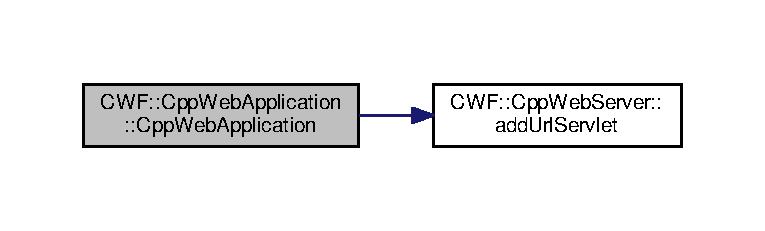
\includegraphics[width=350pt]{class_c_w_f_1_1_cpp_web_application_a7852928699b0de956fa8f6267fef311c_cgraph}
\end{center}
\end{figure}


\hypertarget{class_c_w_f_1_1_cpp_web_application_a29277658a0564c06e2b4116d1527513c}{\index{C\+W\+F\+::\+Cpp\+Web\+Application@{C\+W\+F\+::\+Cpp\+Web\+Application}!````~Cpp\+Web\+Application@{$\sim$\+Cpp\+Web\+Application}}
\index{````~Cpp\+Web\+Application@{$\sim$\+Cpp\+Web\+Application}!C\+W\+F\+::\+Cpp\+Web\+Application@{C\+W\+F\+::\+Cpp\+Web\+Application}}
\subsubsection[{$\sim$\+Cpp\+Web\+Application}]{\setlength{\rightskip}{0pt plus 5cm}C\+W\+F\+::\+Cpp\+Web\+Application\+::$\sim$\+Cpp\+Web\+Application (
\begin{DoxyParamCaption}
{}
\end{DoxyParamCaption}
)}}\label{class_c_w_f_1_1_cpp_web_application_a29277658a0564c06e2b4116d1527513c}


\subsection{Member Function Documentation}
\hypertarget{class_c_w_f_1_1_cpp_web_application_ac9e3224ae26dea5fc61328ae8c49f22d}{\index{C\+W\+F\+::\+Cpp\+Web\+Application@{C\+W\+F\+::\+Cpp\+Web\+Application}!add\+Url\+Servlet@{add\+Url\+Servlet}}
\index{add\+Url\+Servlet@{add\+Url\+Servlet}!C\+W\+F\+::\+Cpp\+Web\+Application@{C\+W\+F\+::\+Cpp\+Web\+Application}}
\subsubsection[{add\+Url\+Servlet}]{\setlength{\rightskip}{0pt plus 5cm}void C\+W\+F\+::\+Cpp\+Web\+Application\+::add\+Url\+Servlet (
\begin{DoxyParamCaption}
\item[{const Q\+String \&}]{url, }
\item[{{\bf Http\+Servlet} $\ast$}]{servlet}
\end{DoxyParamCaption}
)}}\label{class_c_w_f_1_1_cpp_web_application_ac9e3224ae26dea5fc61328ae8c49f22d}


Here is the call graph for this function\+:
\nopagebreak
\begin{figure}[H]
\begin{center}
\leavevmode
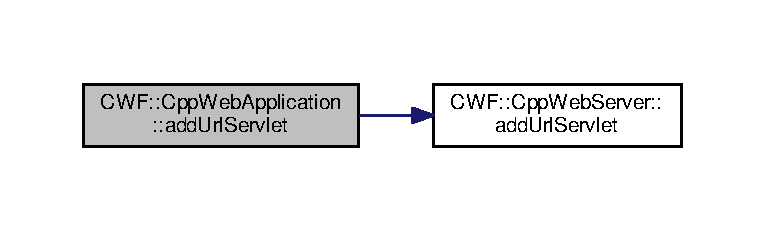
\includegraphics[width=350pt]{class_c_w_f_1_1_cpp_web_application_ac9e3224ae26dea5fc61328ae8c49f22d_cgraph}
\end{center}
\end{figure}


\hypertarget{class_c_w_f_1_1_cpp_web_application_a859f3b5472685da6b2722f9e44b2a2f9}{\index{C\+W\+F\+::\+Cpp\+Web\+Application@{C\+W\+F\+::\+Cpp\+Web\+Application}!start@{start}}
\index{start@{start}!C\+W\+F\+::\+Cpp\+Web\+Application@{C\+W\+F\+::\+Cpp\+Web\+Application}}
\subsubsection[{start}]{\setlength{\rightskip}{0pt plus 5cm}int C\+W\+F\+::\+Cpp\+Web\+Application\+::start (
\begin{DoxyParamCaption}
{}
\end{DoxyParamCaption}
)}}\label{class_c_w_f_1_1_cpp_web_application_a859f3b5472685da6b2722f9e44b2a2f9}


The documentation for this class was generated from the following files\+:\begin{DoxyCompactItemize}
\item 
/home/herik/\+C\+P\+P\+Web\+Framework/\+C\+P\+P\+Web\+Framework/cwf/\hyperlink{cppwebapplication_8h}{cppwebapplication.\+h}\item 
/home/herik/\+C\+P\+P\+Web\+Framework/\+C\+P\+P\+Web\+Framework/cwf/\hyperlink{cppwebapplication_8cpp}{cppwebapplication.\+cpp}\end{DoxyCompactItemize}

\hypertarget{class_c_w_f_1_1_cpp_web_server}{\section{C\+W\+F\+:\+:Cpp\+Web\+Server Class Reference}
\label{class_c_w_f_1_1_cpp_web_server}\index{C\+W\+F\+::\+Cpp\+Web\+Server@{C\+W\+F\+::\+Cpp\+Web\+Server}}
}


The \hyperlink{class_c_w_f_1_1_cpp_web_server}{Cpp\+Web\+Server} class is a H\+T\+T\+P server, responsable to receive and dispatch the requisitions.  




{\ttfamily \#include $<$cppwebserver.\+h$>$}



Inheritance diagram for C\+W\+F\+:\+:Cpp\+Web\+Server\+:
\nopagebreak
\begin{figure}[H]
\begin{center}
\leavevmode
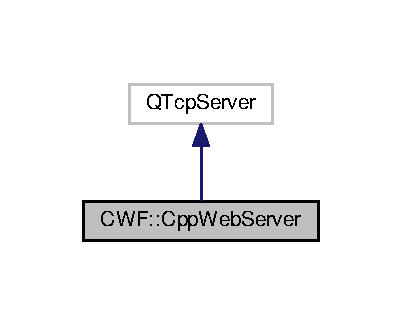
\includegraphics[width=193pt]{class_c_w_f_1_1_cpp_web_server__inherit__graph}
\end{center}
\end{figure}
\subsection*{Public Member Functions}
\begin{DoxyCompactItemize}
\item 
\hyperlink{class_c_w_f_1_1_cpp_web_server_ae462074ec43b8fc04d3239cde4b7f602}{Cpp\+Web\+Server} (\hyperlink{class_c_w_f_1_1_filter}{Filter} $\ast$filter=nullptr)
\begin{DoxyCompactList}\small\item\em Load S\+S\+L configuration, configure the thread pool and the filter. \end{DoxyCompactList}\item 
\hyperlink{class_c_w_f_1_1_cpp_web_server_ab00bb24440420f41b7328a47def0c0cd}{$\sim$\+Cpp\+Web\+Server} ()
\begin{DoxyCompactList}\small\item\em Destroys all servlets and sessions. \end{DoxyCompactList}\item 
void \hyperlink{class_c_w_f_1_1_cpp_web_server_a8acbe56b5d63ded67879f4ed31170c2e}{add\+Url\+Servlet} (const Q\+String \&url, \hyperlink{class_c_w_f_1_1_http_servlet}{Http\+Servlet} $\ast$servlet)
\begin{DoxyCompactList}\small\item\em Hitches a url to a Servlet. \end{DoxyCompactList}\end{DoxyCompactItemize}


\subsection{Detailed Description}
The \hyperlink{class_c_w_f_1_1_cpp_web_server}{Cpp\+Web\+Server} class is a H\+T\+T\+P server, responsable to receive and dispatch the requisitions. 

\subsection{Constructor \& Destructor Documentation}
\hypertarget{class_c_w_f_1_1_cpp_web_server_ae462074ec43b8fc04d3239cde4b7f602}{\index{C\+W\+F\+::\+Cpp\+Web\+Server@{C\+W\+F\+::\+Cpp\+Web\+Server}!Cpp\+Web\+Server@{Cpp\+Web\+Server}}
\index{Cpp\+Web\+Server@{Cpp\+Web\+Server}!C\+W\+F\+::\+Cpp\+Web\+Server@{C\+W\+F\+::\+Cpp\+Web\+Server}}
\subsubsection[{Cpp\+Web\+Server}]{\setlength{\rightskip}{0pt plus 5cm}C\+W\+F\+::\+Cpp\+Web\+Server\+::\+Cpp\+Web\+Server (
\begin{DoxyParamCaption}
\item[{{\bf Filter} $\ast$}]{filter = {\ttfamily nullptr}}
\end{DoxyParamCaption}
)\hspace{0.3cm}{\ttfamily [explicit]}}}\label{class_c_w_f_1_1_cpp_web_server_ae462074ec43b8fc04d3239cde4b7f602}


Load S\+S\+L configuration, configure the thread pool and the filter. 


\begin{DoxyParams}{Parameters}
{\em \hyperlink{class_c_w_f_1_1_filter}{Filter}} & $\ast$filter \+: Install a filter for requests on the server. Optional. \\
\hline
\end{DoxyParams}
\hypertarget{class_c_w_f_1_1_cpp_web_server_ab00bb24440420f41b7328a47def0c0cd}{\index{C\+W\+F\+::\+Cpp\+Web\+Server@{C\+W\+F\+::\+Cpp\+Web\+Server}!````~Cpp\+Web\+Server@{$\sim$\+Cpp\+Web\+Server}}
\index{````~Cpp\+Web\+Server@{$\sim$\+Cpp\+Web\+Server}!C\+W\+F\+::\+Cpp\+Web\+Server@{C\+W\+F\+::\+Cpp\+Web\+Server}}
\subsubsection[{$\sim$\+Cpp\+Web\+Server}]{\setlength{\rightskip}{0pt plus 5cm}C\+W\+F\+::\+Cpp\+Web\+Server\+::$\sim$\+Cpp\+Web\+Server (
\begin{DoxyParamCaption}
{}
\end{DoxyParamCaption}
)}}\label{class_c_w_f_1_1_cpp_web_server_ab00bb24440420f41b7328a47def0c0cd}


Destroys all servlets and sessions. 



\subsection{Member Function Documentation}
\hypertarget{class_c_w_f_1_1_cpp_web_server_a8acbe56b5d63ded67879f4ed31170c2e}{\index{C\+W\+F\+::\+Cpp\+Web\+Server@{C\+W\+F\+::\+Cpp\+Web\+Server}!add\+Url\+Servlet@{add\+Url\+Servlet}}
\index{add\+Url\+Servlet@{add\+Url\+Servlet}!C\+W\+F\+::\+Cpp\+Web\+Server@{C\+W\+F\+::\+Cpp\+Web\+Server}}
\subsubsection[{add\+Url\+Servlet}]{\setlength{\rightskip}{0pt plus 5cm}void C\+W\+F\+::\+Cpp\+Web\+Server\+::add\+Url\+Servlet (
\begin{DoxyParamCaption}
\item[{const Q\+String \&}]{url, }
\item[{{\bf Http\+Servlet} $\ast$}]{servlet}
\end{DoxyParamCaption}
)}}\label{class_c_w_f_1_1_cpp_web_server_a8acbe56b5d63ded67879f4ed31170c2e}


Hitches a url to a Servlet. 


\begin{DoxyParams}{Parameters}
{\em const} & Q\+String \&url \+: Url name. \\
\hline
{\em \hyperlink{class_c_w_f_1_1_http_servlet}{Http\+Servlet}} & $\ast$servlet \+: Servlet that will answer requests made to url. \\
\hline
\end{DoxyParams}


The documentation for this class was generated from the following files\+:\begin{DoxyCompactItemize}
\item 
/home/herik/\+C\+P\+P\+Web\+Framework/\+C\+P\+P\+Web\+Framework/cwf/\hyperlink{cppwebserver_8h}{cppwebserver.\+h}\item 
/home/herik/\+C\+P\+P\+Web\+Framework/\+C\+P\+P\+Web\+Framework/cwf/\hyperlink{cppwebserver_8cpp}{cppwebserver.\+cpp}\end{DoxyCompactItemize}

\hypertarget{class_c_w_f_1_1_cpp_web_servlet}{\section{C\+W\+F\+:\+:Cpp\+Web\+Servlet Class Reference}
\label{class_c_w_f_1_1_cpp_web_servlet}\index{C\+W\+F\+::\+Cpp\+Web\+Servlet@{C\+W\+F\+::\+Cpp\+Web\+Servlet}}
}


This class is responsible for displaying the standard pages of C++ Web Framework\+: index, examples, documentation, ssl and authors.  




{\ttfamily \#include $<$cppwebservlet.\+h$>$}



Inheritance diagram for C\+W\+F\+:\+:Cpp\+Web\+Servlet\+:
\nopagebreak
\begin{figure}[H]
\begin{center}
\leavevmode
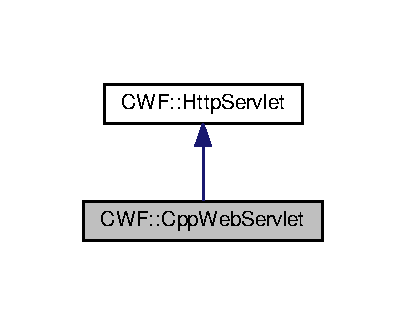
\includegraphics[width=195pt]{class_c_w_f_1_1_cpp_web_servlet__inherit__graph}
\end{center}
\end{figure}
\subsection*{Public Member Functions}
\begin{DoxyCompactItemize}
\item 
void \hyperlink{class_c_w_f_1_1_cpp_web_servlet_a0dca0ce47c2c1d8ecd8d8493773575f8}{do\+Get} (\hyperlink{class_c_w_f_1_1_http_servlet_request}{Http\+Servlet\+Request} \&request, \hyperlink{class_c_w_f_1_1_http_servlet_response}{Http\+Servlet\+Response} \&response) override
\begin{DoxyCompactList}\small\item\em Method overload to answer the requests the system default pages. \end{DoxyCompactList}\end{DoxyCompactItemize}


\subsection{Detailed Description}
This class is responsible for displaying the standard pages of C++ Web Framework\+: index, examples, documentation, ssl and authors. 

\subsection{Member Function Documentation}
\hypertarget{class_c_w_f_1_1_cpp_web_servlet_a0dca0ce47c2c1d8ecd8d8493773575f8}{\index{C\+W\+F\+::\+Cpp\+Web\+Servlet@{C\+W\+F\+::\+Cpp\+Web\+Servlet}!do\+Get@{do\+Get}}
\index{do\+Get@{do\+Get}!C\+W\+F\+::\+Cpp\+Web\+Servlet@{C\+W\+F\+::\+Cpp\+Web\+Servlet}}
\subsubsection[{do\+Get}]{\setlength{\rightskip}{0pt plus 5cm}void C\+W\+F\+::\+Cpp\+Web\+Servlet\+::do\+Get (
\begin{DoxyParamCaption}
\item[{{\bf C\+W\+F\+::\+Http\+Servlet\+Request} \&}]{request, }
\item[{{\bf C\+W\+F\+::\+Http\+Servlet\+Response} \&}]{response}
\end{DoxyParamCaption}
)\hspace{0.3cm}{\ttfamily [override]}, {\ttfamily [virtual]}}}\label{class_c_w_f_1_1_cpp_web_servlet_a0dca0ce47c2c1d8ecd8d8493773575f8}


Method overload to answer the requests the system default pages. 


\begin{DoxyParams}{Parameters}
{\em \hyperlink{class_c_w_f_1_1_http_servlet_request}{Http\+Servlet\+Request}} & \&request \+: Parameter generated by \hyperlink{class_c_w_f_1_1_http_read_request}{Http\+Read\+Request}. \\
\hline
{\em \hyperlink{class_c_w_f_1_1_http_servlet_response}{Http\+Servlet\+Response}} & \&response \+: Parameter generated by \hyperlink{class_c_w_f_1_1_http_read_request}{Http\+Read\+Request}. \\
\hline
\end{DoxyParams}


Reimplemented from \hyperlink{class_c_w_f_1_1_http_servlet_ad05501d3611f28b20d2c045515119f20}{C\+W\+F\+::\+Http\+Servlet}.



The documentation for this class was generated from the following files\+:\begin{DoxyCompactItemize}
\item 
/home/herik/\+C\+P\+P\+Web\+Framework/\+C\+P\+P\+Web\+Framework/cwf/\hyperlink{cppwebservlet_8h}{cppwebservlet.\+h}\item 
/home/herik/\+C\+P\+P\+Web\+Framework/\+C\+P\+P\+Web\+Framework/cwf/\hyperlink{cppwebservlet_8cpp}{cppwebservlet.\+cpp}\end{DoxyCompactItemize}

\hypertarget{class_c_w_f_1_1_c_s_t_l_compiler}{\section{C\+W\+F\+:\+:C\+S\+T\+L\+Compiler Class Reference}
\label{class_c_w_f_1_1_c_s_t_l_compiler}\index{C\+W\+F\+::\+C\+S\+T\+L\+Compiler@{C\+W\+F\+::\+C\+S\+T\+L\+Compiler}}
}


{\ttfamily \#include $<$cstlcompiler.\+h$>$}

\subsection*{Public Member Functions}
\begin{DoxyCompactItemize}
\item 
\hyperlink{class_c_w_f_1_1_c_s_t_l_compiler_a58e8247e5bd5b41a175aee75b9ddf6fc}{C\+S\+T\+L\+Compiler} (const Q\+Byte\+Array \&str, Q\+Map$<$ Q\+String, Q\+Object $\ast$ $>$ \&objects, bool is\+Str\+File\+Name=true)
\item 
Q\+Byte\+Array \hyperlink{class_c_w_f_1_1_c_s_t_l_compiler_aa28ba20afd8d5ff643a773d7fa5c0b54}{output} ()
\end{DoxyCompactItemize}


\subsection{Constructor \& Destructor Documentation}
\hypertarget{class_c_w_f_1_1_c_s_t_l_compiler_a58e8247e5bd5b41a175aee75b9ddf6fc}{\index{C\+W\+F\+::\+C\+S\+T\+L\+Compiler@{C\+W\+F\+::\+C\+S\+T\+L\+Compiler}!C\+S\+T\+L\+Compiler@{C\+S\+T\+L\+Compiler}}
\index{C\+S\+T\+L\+Compiler@{C\+S\+T\+L\+Compiler}!C\+W\+F\+::\+C\+S\+T\+L\+Compiler@{C\+W\+F\+::\+C\+S\+T\+L\+Compiler}}
\subsubsection[{C\+S\+T\+L\+Compiler}]{\setlength{\rightskip}{0pt plus 5cm}C\+W\+F\+::\+C\+S\+T\+L\+Compiler\+::\+C\+S\+T\+L\+Compiler (
\begin{DoxyParamCaption}
\item[{const Q\+Byte\+Array \&}]{str, }
\item[{Q\+Map$<$ Q\+String, Q\+Object $\ast$ $>$ \&}]{objects, }
\item[{bool}]{is\+Str\+File\+Name = {\ttfamily true}}
\end{DoxyParamCaption}
)}}\label{class_c_w_f_1_1_c_s_t_l_compiler_a58e8247e5bd5b41a175aee75b9ddf6fc}


\subsection{Member Function Documentation}
\hypertarget{class_c_w_f_1_1_c_s_t_l_compiler_aa28ba20afd8d5ff643a773d7fa5c0b54}{\index{C\+W\+F\+::\+C\+S\+T\+L\+Compiler@{C\+W\+F\+::\+C\+S\+T\+L\+Compiler}!output@{output}}
\index{output@{output}!C\+W\+F\+::\+C\+S\+T\+L\+Compiler@{C\+W\+F\+::\+C\+S\+T\+L\+Compiler}}
\subsubsection[{output}]{\setlength{\rightskip}{0pt plus 5cm}Q\+Byte\+Array C\+W\+F\+::\+C\+S\+T\+L\+Compiler\+::output (
\begin{DoxyParamCaption}
{}
\end{DoxyParamCaption}
)}}\label{class_c_w_f_1_1_c_s_t_l_compiler_aa28ba20afd8d5ff643a773d7fa5c0b54}


The documentation for this class was generated from the following files\+:\begin{DoxyCompactItemize}
\item 
/home/herik/\+C\+P\+P\+Web\+Framework/\+C\+P\+P\+Web\+Framework/cwf/\hyperlink{cstlcompiler_8h}{cstlcompiler.\+h}\item 
/home/herik/\+C\+P\+P\+Web\+Framework/\+C\+P\+P\+Web\+Framework/cwf/\hyperlink{cstlcompiler_8cpp}{cstlcompiler.\+cpp}\end{DoxyCompactItemize}

\hypertarget{class_c_w_f_1_1_c_s_t_l_compiler_attributes}{\section{C\+W\+F\+:\+:C\+S\+T\+L\+Compiler\+Attributes Class Reference}
\label{class_c_w_f_1_1_c_s_t_l_compiler_attributes}\index{C\+W\+F\+::\+C\+S\+T\+L\+Compiler\+Attributes@{C\+W\+F\+::\+C\+S\+T\+L\+Compiler\+Attributes}}
}


This class search for expressions(\#\{obj.\+get\}) and compiles it.  




{\ttfamily \#include $<$cstlcompilerattributes.\+h$>$}

\subsection*{Public Member Functions}
\begin{DoxyCompactItemize}
\item 
\hyperlink{class_c_w_f_1_1_c_s_t_l_compiler_attributes_a666a7c7dec101d1313027c1037255446}{C\+S\+T\+L\+Compiler\+Attributes} (Q\+Map$<$ Q\+String, Q\+Object $\ast$ $>$ \&objects)
\item 
Q\+String \hyperlink{class_c_w_f_1_1_c_s_t_l_compiler_attributes_a6c09d18bbc92ae092db120385a7d40de}{build\+Attributes} (Q\+Map$<$ Q\+String, Q\+String $>$ \&attr, bool key\+Value=true)
\item 
void \hyperlink{class_c_w_f_1_1_c_s_t_l_compiler_attributes_a5eccb899f04af2c269845f1e86e07813}{compile\+Attributes} (Q\+Map$<$ Q\+String, Q\+String $>$ \&attr)
\item 
void \hyperlink{class_c_w_f_1_1_c_s_t_l_compiler_attributes_a482a81daba4f114b75445ac54868d572}{compile} (Q\+String \&text, Q\+String \&out\+Put\+Text)
\item 
Q\+Map$<$ Q\+String, Q\+String $>$ \hyperlink{class_c_w_f_1_1_c_s_t_l_compiler_attributes_a4cbbe112e36b86ef01401e1b62804d57}{get\+Attributes} (const Q\+Xml\+Stream\+Attributes \&attributes)
\end{DoxyCompactItemize}


\subsection{Detailed Description}
This class search for expressions(\#\{obj.\+get\}) and compiles it. 

\subsection{Constructor \& Destructor Documentation}
\hypertarget{class_c_w_f_1_1_c_s_t_l_compiler_attributes_a666a7c7dec101d1313027c1037255446}{\index{C\+W\+F\+::\+C\+S\+T\+L\+Compiler\+Attributes@{C\+W\+F\+::\+C\+S\+T\+L\+Compiler\+Attributes}!C\+S\+T\+L\+Compiler\+Attributes@{C\+S\+T\+L\+Compiler\+Attributes}}
\index{C\+S\+T\+L\+Compiler\+Attributes@{C\+S\+T\+L\+Compiler\+Attributes}!C\+W\+F\+::\+C\+S\+T\+L\+Compiler\+Attributes@{C\+W\+F\+::\+C\+S\+T\+L\+Compiler\+Attributes}}
\subsubsection[{C\+S\+T\+L\+Compiler\+Attributes}]{\setlength{\rightskip}{0pt plus 5cm}C\+W\+F\+::\+C\+S\+T\+L\+Compiler\+Attributes\+::\+C\+S\+T\+L\+Compiler\+Attributes (
\begin{DoxyParamCaption}
\item[{Q\+Map$<$ Q\+String, Q\+Object $\ast$ $>$ \&}]{objects}
\end{DoxyParamCaption}
)}}\label{class_c_w_f_1_1_c_s_t_l_compiler_attributes_a666a7c7dec101d1313027c1037255446}


\subsection{Member Function Documentation}
\hypertarget{class_c_w_f_1_1_c_s_t_l_compiler_attributes_a6c09d18bbc92ae092db120385a7d40de}{\index{C\+W\+F\+::\+C\+S\+T\+L\+Compiler\+Attributes@{C\+W\+F\+::\+C\+S\+T\+L\+Compiler\+Attributes}!build\+Attributes@{build\+Attributes}}
\index{build\+Attributes@{build\+Attributes}!C\+W\+F\+::\+C\+S\+T\+L\+Compiler\+Attributes@{C\+W\+F\+::\+C\+S\+T\+L\+Compiler\+Attributes}}
\subsubsection[{build\+Attributes}]{\setlength{\rightskip}{0pt plus 5cm}Q\+String C\+W\+F\+::\+C\+S\+T\+L\+Compiler\+Attributes\+::build\+Attributes (
\begin{DoxyParamCaption}
\item[{Q\+Map$<$ Q\+String, Q\+String $>$ \&}]{attr, }
\item[{bool}]{key\+Value = {\ttfamily true}}
\end{DoxyParamCaption}
)}}\label{class_c_w_f_1_1_c_s_t_l_compiler_attributes_a6c09d18bbc92ae092db120385a7d40de}
\hypertarget{class_c_w_f_1_1_c_s_t_l_compiler_attributes_a482a81daba4f114b75445ac54868d572}{\index{C\+W\+F\+::\+C\+S\+T\+L\+Compiler\+Attributes@{C\+W\+F\+::\+C\+S\+T\+L\+Compiler\+Attributes}!compile@{compile}}
\index{compile@{compile}!C\+W\+F\+::\+C\+S\+T\+L\+Compiler\+Attributes@{C\+W\+F\+::\+C\+S\+T\+L\+Compiler\+Attributes}}
\subsubsection[{compile}]{\setlength{\rightskip}{0pt plus 5cm}void C\+W\+F\+::\+C\+S\+T\+L\+Compiler\+Attributes\+::compile (
\begin{DoxyParamCaption}
\item[{Q\+String \&}]{text, }
\item[{Q\+String \&}]{out\+Put\+Text}
\end{DoxyParamCaption}
)}}\label{class_c_w_f_1_1_c_s_t_l_compiler_attributes_a482a81daba4f114b75445ac54868d572}
\hypertarget{class_c_w_f_1_1_c_s_t_l_compiler_attributes_a5eccb899f04af2c269845f1e86e07813}{\index{C\+W\+F\+::\+C\+S\+T\+L\+Compiler\+Attributes@{C\+W\+F\+::\+C\+S\+T\+L\+Compiler\+Attributes}!compile\+Attributes@{compile\+Attributes}}
\index{compile\+Attributes@{compile\+Attributes}!C\+W\+F\+::\+C\+S\+T\+L\+Compiler\+Attributes@{C\+W\+F\+::\+C\+S\+T\+L\+Compiler\+Attributes}}
\subsubsection[{compile\+Attributes}]{\setlength{\rightskip}{0pt plus 5cm}void C\+W\+F\+::\+C\+S\+T\+L\+Compiler\+Attributes\+::compile\+Attributes (
\begin{DoxyParamCaption}
\item[{Q\+Map$<$ Q\+String, Q\+String $>$ \&}]{attr}
\end{DoxyParamCaption}
)}}\label{class_c_w_f_1_1_c_s_t_l_compiler_attributes_a5eccb899f04af2c269845f1e86e07813}
\hypertarget{class_c_w_f_1_1_c_s_t_l_compiler_attributes_a4cbbe112e36b86ef01401e1b62804d57}{\index{C\+W\+F\+::\+C\+S\+T\+L\+Compiler\+Attributes@{C\+W\+F\+::\+C\+S\+T\+L\+Compiler\+Attributes}!get\+Attributes@{get\+Attributes}}
\index{get\+Attributes@{get\+Attributes}!C\+W\+F\+::\+C\+S\+T\+L\+Compiler\+Attributes@{C\+W\+F\+::\+C\+S\+T\+L\+Compiler\+Attributes}}
\subsubsection[{get\+Attributes}]{\setlength{\rightskip}{0pt plus 5cm}Q\+Map$<$ Q\+String, Q\+String $>$ C\+W\+F\+::\+C\+S\+T\+L\+Compiler\+Attributes\+::get\+Attributes (
\begin{DoxyParamCaption}
\item[{const Q\+Xml\+Stream\+Attributes \&}]{attributes}
\end{DoxyParamCaption}
)}}\label{class_c_w_f_1_1_c_s_t_l_compiler_attributes_a4cbbe112e36b86ef01401e1b62804d57}


The documentation for this class was generated from the following files\+:\begin{DoxyCompactItemize}
\item 
/home/herik/\+C\+P\+P\+Web\+Framework/\+C\+P\+P\+Web\+Framework/cwf/\hyperlink{cstlcompilerattributes_8h}{cstlcompilerattributes.\+h}\item 
/home/herik/\+C\+P\+P\+Web\+Framework/\+C\+P\+P\+Web\+Framework/cwf/\hyperlink{cstlcompilerattributes_8cpp}{cstlcompilerattributes.\+cpp}\end{DoxyCompactItemize}

\hypertarget{class_c_w_f_1_1_c_s_t_l_compiler_for}{\section{C\+W\+F\+:\+:C\+S\+T\+L\+Compiler\+For Class Reference}
\label{class_c_w_f_1_1_c_s_t_l_compiler_for}\index{C\+W\+F\+::\+C\+S\+T\+L\+Compiler\+For@{C\+W\+F\+::\+C\+S\+T\+L\+Compiler\+For}}
}


{\ttfamily \#include $<$cstlcompilerfor.\+h$>$}

\subsection*{Public Member Functions}
\begin{DoxyCompactItemize}
\item 
\hyperlink{class_c_w_f_1_1_c_s_t_l_compiler_for_a43830cd5b6f25d5ec2fd156b141c04f3}{C\+S\+T\+L\+Compiler\+For} (const Q\+Xml\+Stream\+Attributes \&attr)
\end{DoxyCompactItemize}
\subsection*{Public Attributes}
\begin{DoxyCompactItemize}
\item 
Q\+Map$<$ Q\+String, Q\+String $>$ \hyperlink{class_c_w_f_1_1_c_s_t_l_compiler_for_ab90c925cb83704f2e22f19cdf9d48974}{attributes}
\end{DoxyCompactItemize}


\subsection{Constructor \& Destructor Documentation}
\hypertarget{class_c_w_f_1_1_c_s_t_l_compiler_for_a43830cd5b6f25d5ec2fd156b141c04f3}{\index{C\+W\+F\+::\+C\+S\+T\+L\+Compiler\+For@{C\+W\+F\+::\+C\+S\+T\+L\+Compiler\+For}!C\+S\+T\+L\+Compiler\+For@{C\+S\+T\+L\+Compiler\+For}}
\index{C\+S\+T\+L\+Compiler\+For@{C\+S\+T\+L\+Compiler\+For}!C\+W\+F\+::\+C\+S\+T\+L\+Compiler\+For@{C\+W\+F\+::\+C\+S\+T\+L\+Compiler\+For}}
\subsubsection[{C\+S\+T\+L\+Compiler\+For}]{\setlength{\rightskip}{0pt plus 5cm}C\+W\+F\+::\+C\+S\+T\+L\+Compiler\+For\+::\+C\+S\+T\+L\+Compiler\+For (
\begin{DoxyParamCaption}
\item[{const Q\+Xml\+Stream\+Attributes \&}]{attr}
\end{DoxyParamCaption}
)}}\label{class_c_w_f_1_1_c_s_t_l_compiler_for_a43830cd5b6f25d5ec2fd156b141c04f3}


\subsection{Member Data Documentation}
\hypertarget{class_c_w_f_1_1_c_s_t_l_compiler_for_ab90c925cb83704f2e22f19cdf9d48974}{\index{C\+W\+F\+::\+C\+S\+T\+L\+Compiler\+For@{C\+W\+F\+::\+C\+S\+T\+L\+Compiler\+For}!attributes@{attributes}}
\index{attributes@{attributes}!C\+W\+F\+::\+C\+S\+T\+L\+Compiler\+For@{C\+W\+F\+::\+C\+S\+T\+L\+Compiler\+For}}
\subsubsection[{attributes}]{\setlength{\rightskip}{0pt plus 5cm}Q\+Map$<$Q\+String, Q\+String$>$ C\+W\+F\+::\+C\+S\+T\+L\+Compiler\+For\+::attributes}}\label{class_c_w_f_1_1_c_s_t_l_compiler_for_ab90c925cb83704f2e22f19cdf9d48974}


The documentation for this class was generated from the following files\+:\begin{DoxyCompactItemize}
\item 
/home/herik/\+C\+P\+P\+Web\+Framework/\+C\+P\+P\+Web\+Framework/cwf/\hyperlink{cstlcompilerfor_8h}{cstlcompilerfor.\+h}\item 
/home/herik/\+C\+P\+P\+Web\+Framework/\+C\+P\+P\+Web\+Framework/cwf/\hyperlink{cstlcompilerfor_8cpp}{cstlcompilerfor.\+cpp}\end{DoxyCompactItemize}

\hypertarget{class_c_w_f_1_1_c_s_t_l_compiler_if}{\section{C\+W\+F\+:\+:C\+S\+T\+L\+Compiler\+If Class Reference}
\label{class_c_w_f_1_1_c_s_t_l_compiler_if}\index{C\+W\+F\+::\+C\+S\+T\+L\+Compiler\+If@{C\+W\+F\+::\+C\+S\+T\+L\+Compiler\+If}}
}


{\ttfamily \#include $<$cstlcompilerif.\+h$>$}

\subsection*{Public Member Functions}
\begin{DoxyCompactItemize}
\item 
\hyperlink{class_c_w_f_1_1_c_s_t_l_compiler_if_a6fff1cab935cc881a8d444c51e1d1163}{C\+S\+T\+L\+Compiler\+If} (const Q\+Xml\+Stream\+Attributes \&attr)
\end{DoxyCompactItemize}
\subsection*{Public Attributes}
\begin{DoxyCompactItemize}
\item 
Q\+Map$<$ Q\+String, Q\+String $>$ \hyperlink{class_c_w_f_1_1_c_s_t_l_compiler_if_a63f36fca57a21e38d555b6e52173ef0a}{attributes}
\end{DoxyCompactItemize}


\subsection{Constructor \& Destructor Documentation}
\hypertarget{class_c_w_f_1_1_c_s_t_l_compiler_if_a6fff1cab935cc881a8d444c51e1d1163}{\index{C\+W\+F\+::\+C\+S\+T\+L\+Compiler\+If@{C\+W\+F\+::\+C\+S\+T\+L\+Compiler\+If}!C\+S\+T\+L\+Compiler\+If@{C\+S\+T\+L\+Compiler\+If}}
\index{C\+S\+T\+L\+Compiler\+If@{C\+S\+T\+L\+Compiler\+If}!C\+W\+F\+::\+C\+S\+T\+L\+Compiler\+If@{C\+W\+F\+::\+C\+S\+T\+L\+Compiler\+If}}
\subsubsection[{C\+S\+T\+L\+Compiler\+If}]{\setlength{\rightskip}{0pt plus 5cm}C\+W\+F\+::\+C\+S\+T\+L\+Compiler\+If\+::\+C\+S\+T\+L\+Compiler\+If (
\begin{DoxyParamCaption}
\item[{const Q\+Xml\+Stream\+Attributes \&}]{attr}
\end{DoxyParamCaption}
)}}\label{class_c_w_f_1_1_c_s_t_l_compiler_if_a6fff1cab935cc881a8d444c51e1d1163}


\subsection{Member Data Documentation}
\hypertarget{class_c_w_f_1_1_c_s_t_l_compiler_if_a63f36fca57a21e38d555b6e52173ef0a}{\index{C\+W\+F\+::\+C\+S\+T\+L\+Compiler\+If@{C\+W\+F\+::\+C\+S\+T\+L\+Compiler\+If}!attributes@{attributes}}
\index{attributes@{attributes}!C\+W\+F\+::\+C\+S\+T\+L\+Compiler\+If@{C\+W\+F\+::\+C\+S\+T\+L\+Compiler\+If}}
\subsubsection[{attributes}]{\setlength{\rightskip}{0pt plus 5cm}Q\+Map$<$Q\+String, Q\+String$>$ C\+W\+F\+::\+C\+S\+T\+L\+Compiler\+If\+::attributes}}\label{class_c_w_f_1_1_c_s_t_l_compiler_if_a63f36fca57a21e38d555b6e52173ef0a}


The documentation for this class was generated from the following files\+:\begin{DoxyCompactItemize}
\item 
/home/herik/\+C\+P\+P\+Web\+Framework/\+C\+P\+P\+Web\+Framework/cwf/\hyperlink{cstlcompilerif_8h}{cstlcompilerif.\+h}\item 
/home/herik/\+C\+P\+P\+Web\+Framework/\+C\+P\+P\+Web\+Framework/cwf/\hyperlink{cstlcompilerif_8cpp}{cstlcompilerif.\+cpp}\end{DoxyCompactItemize}

\hypertarget{class_c_w_f_1_1_c_s_t_l_compiler_object}{\section{C\+W\+F\+:\+:C\+S\+T\+L\+Compiler\+Object Class Reference}
\label{class_c_w_f_1_1_c_s_t_l_compiler_object}\index{C\+W\+F\+::\+C\+S\+T\+L\+Compiler\+Object@{C\+W\+F\+::\+C\+S\+T\+L\+Compiler\+Object}}
}


{\ttfamily \#include $<$cstlcompilerobject.\+h$>$}



Inheritance diagram for C\+W\+F\+:\+:C\+S\+T\+L\+Compiler\+Object\+:
\nopagebreak
\begin{figure}[H]
\begin{center}
\leavevmode
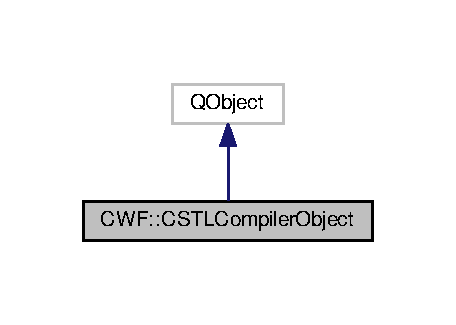
\includegraphics[width=219pt]{class_c_w_f_1_1_c_s_t_l_compiler_object__inherit__graph}
\end{center}
\end{figure}
\subsection*{Public Slots}
\begin{DoxyCompactItemize}
\item 
Q\+String \hyperlink{class_c_w_f_1_1_c_s_t_l_compiler_object_a92137c536b356e4f6eeb76a3c1b65e54}{get\+Value} () const 
\item 
void \hyperlink{class_c_w_f_1_1_c_s_t_l_compiler_object_acf0a476bd687e47edb169c480193654f}{set\+Value} (const Q\+String \&value)
\item 
Q\+String \hyperlink{class_c_w_f_1_1_c_s_t_l_compiler_object_ac7cd5fe07f3b71e0d4b6342db1a4cd29}{get\+Type} () const 
\item 
void \hyperlink{class_c_w_f_1_1_c_s_t_l_compiler_object_a51e99c46daee9cb1f14088d69d2d4e0e}{set\+Type} (const Q\+String \&value)
\end{DoxyCompactItemize}
\subsection*{Public Member Functions}
\begin{DoxyCompactItemize}
\item 
\hyperlink{class_c_w_f_1_1_c_s_t_l_compiler_object_a1c20bd083beceaaef00fcaf10f9e061c}{C\+S\+T\+L\+Compiler\+Object} (Q\+Object $\ast$parent=0)
\end{DoxyCompactItemize}


\subsection{Constructor \& Destructor Documentation}
\hypertarget{class_c_w_f_1_1_c_s_t_l_compiler_object_a1c20bd083beceaaef00fcaf10f9e061c}{\index{C\+W\+F\+::\+C\+S\+T\+L\+Compiler\+Object@{C\+W\+F\+::\+C\+S\+T\+L\+Compiler\+Object}!C\+S\+T\+L\+Compiler\+Object@{C\+S\+T\+L\+Compiler\+Object}}
\index{C\+S\+T\+L\+Compiler\+Object@{C\+S\+T\+L\+Compiler\+Object}!C\+W\+F\+::\+C\+S\+T\+L\+Compiler\+Object@{C\+W\+F\+::\+C\+S\+T\+L\+Compiler\+Object}}
\subsubsection[{C\+S\+T\+L\+Compiler\+Object}]{\setlength{\rightskip}{0pt plus 5cm}C\+W\+F\+::\+C\+S\+T\+L\+Compiler\+Object\+::\+C\+S\+T\+L\+Compiler\+Object (
\begin{DoxyParamCaption}
\item[{Q\+Object $\ast$}]{parent = {\ttfamily 0}}
\end{DoxyParamCaption}
)}}\label{class_c_w_f_1_1_c_s_t_l_compiler_object_a1c20bd083beceaaef00fcaf10f9e061c}


\subsection{Member Function Documentation}
\hypertarget{class_c_w_f_1_1_c_s_t_l_compiler_object_ac7cd5fe07f3b71e0d4b6342db1a4cd29}{\index{C\+W\+F\+::\+C\+S\+T\+L\+Compiler\+Object@{C\+W\+F\+::\+C\+S\+T\+L\+Compiler\+Object}!get\+Type@{get\+Type}}
\index{get\+Type@{get\+Type}!C\+W\+F\+::\+C\+S\+T\+L\+Compiler\+Object@{C\+W\+F\+::\+C\+S\+T\+L\+Compiler\+Object}}
\subsubsection[{get\+Type}]{\setlength{\rightskip}{0pt plus 5cm}Q\+String C\+W\+F\+::\+C\+S\+T\+L\+Compiler\+Object\+::get\+Type (
\begin{DoxyParamCaption}
{}
\end{DoxyParamCaption}
) const\hspace{0.3cm}{\ttfamily [slot]}}}\label{class_c_w_f_1_1_c_s_t_l_compiler_object_ac7cd5fe07f3b71e0d4b6342db1a4cd29}
\hypertarget{class_c_w_f_1_1_c_s_t_l_compiler_object_a92137c536b356e4f6eeb76a3c1b65e54}{\index{C\+W\+F\+::\+C\+S\+T\+L\+Compiler\+Object@{C\+W\+F\+::\+C\+S\+T\+L\+Compiler\+Object}!get\+Value@{get\+Value}}
\index{get\+Value@{get\+Value}!C\+W\+F\+::\+C\+S\+T\+L\+Compiler\+Object@{C\+W\+F\+::\+C\+S\+T\+L\+Compiler\+Object}}
\subsubsection[{get\+Value}]{\setlength{\rightskip}{0pt plus 5cm}Q\+String C\+W\+F\+::\+C\+S\+T\+L\+Compiler\+Object\+::get\+Value (
\begin{DoxyParamCaption}
{}
\end{DoxyParamCaption}
) const\hspace{0.3cm}{\ttfamily [slot]}}}\label{class_c_w_f_1_1_c_s_t_l_compiler_object_a92137c536b356e4f6eeb76a3c1b65e54}
\hypertarget{class_c_w_f_1_1_c_s_t_l_compiler_object_a51e99c46daee9cb1f14088d69d2d4e0e}{\index{C\+W\+F\+::\+C\+S\+T\+L\+Compiler\+Object@{C\+W\+F\+::\+C\+S\+T\+L\+Compiler\+Object}!set\+Type@{set\+Type}}
\index{set\+Type@{set\+Type}!C\+W\+F\+::\+C\+S\+T\+L\+Compiler\+Object@{C\+W\+F\+::\+C\+S\+T\+L\+Compiler\+Object}}
\subsubsection[{set\+Type}]{\setlength{\rightskip}{0pt plus 5cm}void C\+W\+F\+::\+C\+S\+T\+L\+Compiler\+Object\+::set\+Type (
\begin{DoxyParamCaption}
\item[{const Q\+String \&}]{value}
\end{DoxyParamCaption}
)\hspace{0.3cm}{\ttfamily [slot]}}}\label{class_c_w_f_1_1_c_s_t_l_compiler_object_a51e99c46daee9cb1f14088d69d2d4e0e}
\hypertarget{class_c_w_f_1_1_c_s_t_l_compiler_object_acf0a476bd687e47edb169c480193654f}{\index{C\+W\+F\+::\+C\+S\+T\+L\+Compiler\+Object@{C\+W\+F\+::\+C\+S\+T\+L\+Compiler\+Object}!set\+Value@{set\+Value}}
\index{set\+Value@{set\+Value}!C\+W\+F\+::\+C\+S\+T\+L\+Compiler\+Object@{C\+W\+F\+::\+C\+S\+T\+L\+Compiler\+Object}}
\subsubsection[{set\+Value}]{\setlength{\rightskip}{0pt plus 5cm}void C\+W\+F\+::\+C\+S\+T\+L\+Compiler\+Object\+::set\+Value (
\begin{DoxyParamCaption}
\item[{const Q\+String \&}]{value}
\end{DoxyParamCaption}
)\hspace{0.3cm}{\ttfamily [slot]}}}\label{class_c_w_f_1_1_c_s_t_l_compiler_object_acf0a476bd687e47edb169c480193654f}


The documentation for this class was generated from the following files\+:\begin{DoxyCompactItemize}
\item 
/home/herik/\+C\+P\+P\+Web\+Framework/\+C\+P\+P\+Web\+Framework/cwf/\hyperlink{cstlcompilerobject_8h}{cstlcompilerobject.\+h}\item 
/home/herik/\+C\+P\+P\+Web\+Framework/\+C\+P\+P\+Web\+Framework/cwf/\hyperlink{cstlcompilerobject_8cpp}{cstlcompilerobject.\+cpp}\end{DoxyCompactItemize}

\hypertarget{class_c_w_f_1_1_file_manager}{\section{C\+W\+F\+:\+:File\+Manager Class Reference}
\label{class_c_w_f_1_1_file_manager}\index{C\+W\+F\+::\+File\+Manager@{C\+W\+F\+::\+File\+Manager}}
}


The \hyperlink{class_c_w_f_1_1_file_manager}{File\+Manager} class can manage file's name.  




{\ttfamily \#include $<$filemanager.\+h$>$}

\subsection*{Public Member Functions}
\begin{DoxyCompactItemize}
\item 
Q\+String \hyperlink{class_c_w_f_1_1_file_manager_af431982f5da9772dc851a792ca42cf1d}{extract} (Q\+String \&name, char ch) const 
\item 
Q\+String \hyperlink{class_c_w_f_1_1_file_manager_a435ffe313b96261567da05806d38bacc}{file\+Name} (Q\+String \&name) const 
\item 
Q\+String \hyperlink{class_c_w_f_1_1_file_manager_a6b0dd898b161a1fb129aa7d488674b3a}{file\+Extention} (Q\+String \&name) const 
\item 
void \hyperlink{class_c_w_f_1_1_file_manager_a0b00584a292008515b686c67187bac13}{remove\+Last\+Bar} (Q\+String \&path) const 
\item 
void \hyperlink{class_c_w_f_1_1_file_manager_aa7918801a52bd8789239542b1c368889}{remove\+First\+Bar} (Q\+String \&path) const 
\item 
void \hyperlink{class_c_w_f_1_1_file_manager_af1c46c869cd3eece80c937556ecef9c8}{put\+First\+Bar} (Q\+String \&path) const 
\item 
Q\+Byte\+Array \hyperlink{class_c_w_f_1_1_file_manager_ad0e948a2e72ffa137027a3daa6055747}{read\+All} (const Q\+String \&\hyperlink{class_c_w_f_1_1_file_manager_a435ffe313b96261567da05806d38bacc}{file\+Name}, Q\+File\+Device\+::\+File\+Error \&file\+Erro) const 
\end{DoxyCompactItemize}


\subsection{Detailed Description}
The \hyperlink{class_c_w_f_1_1_file_manager}{File\+Manager} class can manage file's name. 

\subsection{Member Function Documentation}
\hypertarget{class_c_w_f_1_1_file_manager_af431982f5da9772dc851a792ca42cf1d}{\index{C\+W\+F\+::\+File\+Manager@{C\+W\+F\+::\+File\+Manager}!extract@{extract}}
\index{extract@{extract}!C\+W\+F\+::\+File\+Manager@{C\+W\+F\+::\+File\+Manager}}
\subsubsection[{extract}]{\setlength{\rightskip}{0pt plus 5cm}Q\+String C\+W\+F\+::\+File\+Manager\+::extract (
\begin{DoxyParamCaption}
\item[{Q\+String \&}]{name, }
\item[{char}]{ch}
\end{DoxyParamCaption}
) const}}\label{class_c_w_f_1_1_file_manager_af431982f5da9772dc851a792ca42cf1d}


Here is the caller graph for this function\+:
\nopagebreak
\begin{figure}[H]
\begin{center}
\leavevmode
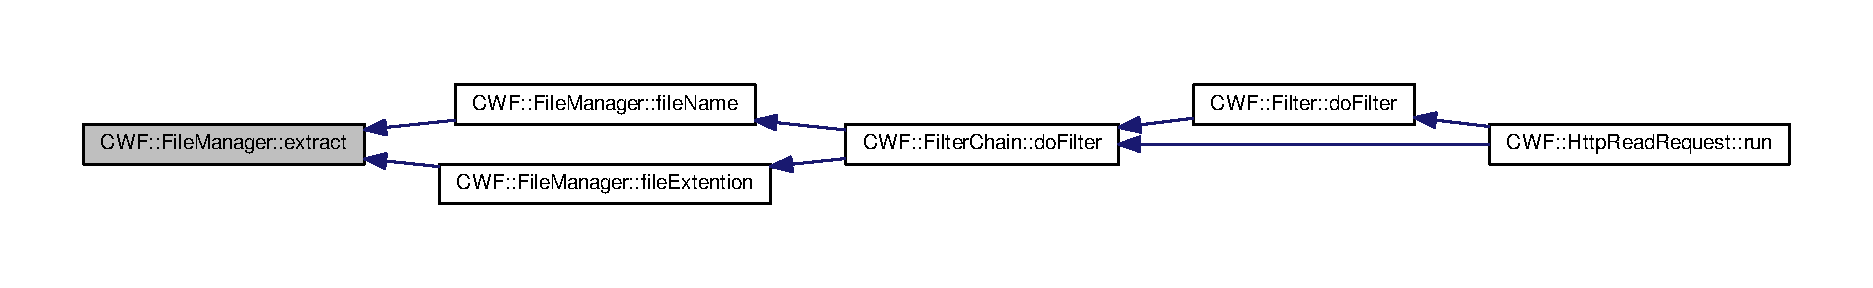
\includegraphics[width=350pt]{class_c_w_f_1_1_file_manager_af431982f5da9772dc851a792ca42cf1d_icgraph}
\end{center}
\end{figure}


\hypertarget{class_c_w_f_1_1_file_manager_a6b0dd898b161a1fb129aa7d488674b3a}{\index{C\+W\+F\+::\+File\+Manager@{C\+W\+F\+::\+File\+Manager}!file\+Extention@{file\+Extention}}
\index{file\+Extention@{file\+Extention}!C\+W\+F\+::\+File\+Manager@{C\+W\+F\+::\+File\+Manager}}
\subsubsection[{file\+Extention}]{\setlength{\rightskip}{0pt plus 5cm}Q\+String C\+W\+F\+::\+File\+Manager\+::file\+Extention (
\begin{DoxyParamCaption}
\item[{Q\+String \&}]{name}
\end{DoxyParamCaption}
) const}}\label{class_c_w_f_1_1_file_manager_a6b0dd898b161a1fb129aa7d488674b3a}


Here is the call graph for this function\+:
\nopagebreak
\begin{figure}[H]
\begin{center}
\leavevmode
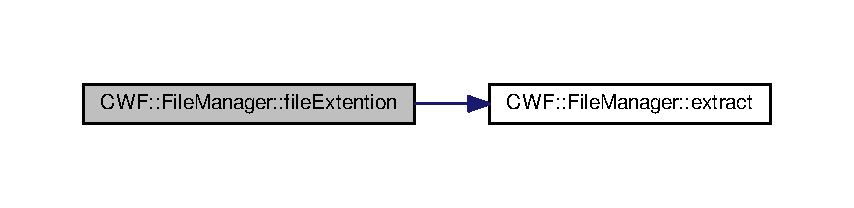
\includegraphics[width=350pt]{class_c_w_f_1_1_file_manager_a6b0dd898b161a1fb129aa7d488674b3a_cgraph}
\end{center}
\end{figure}




Here is the caller graph for this function\+:
\nopagebreak
\begin{figure}[H]
\begin{center}
\leavevmode
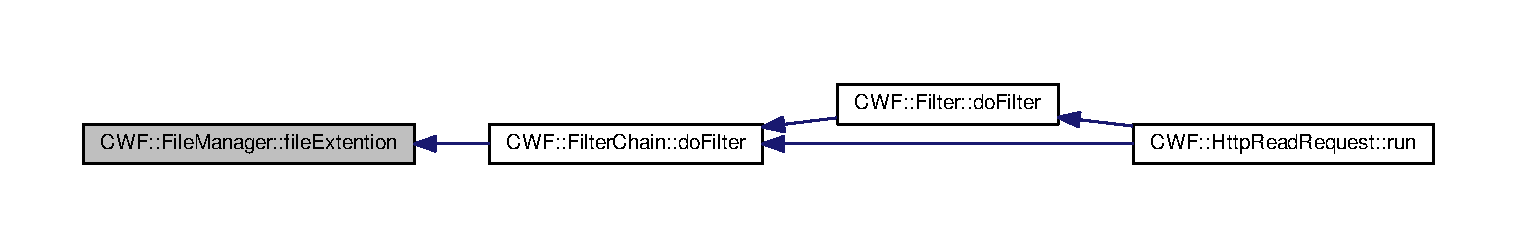
\includegraphics[width=350pt]{class_c_w_f_1_1_file_manager_a6b0dd898b161a1fb129aa7d488674b3a_icgraph}
\end{center}
\end{figure}


\hypertarget{class_c_w_f_1_1_file_manager_a435ffe313b96261567da05806d38bacc}{\index{C\+W\+F\+::\+File\+Manager@{C\+W\+F\+::\+File\+Manager}!file\+Name@{file\+Name}}
\index{file\+Name@{file\+Name}!C\+W\+F\+::\+File\+Manager@{C\+W\+F\+::\+File\+Manager}}
\subsubsection[{file\+Name}]{\setlength{\rightskip}{0pt plus 5cm}Q\+String C\+W\+F\+::\+File\+Manager\+::file\+Name (
\begin{DoxyParamCaption}
\item[{Q\+String \&}]{name}
\end{DoxyParamCaption}
) const}}\label{class_c_w_f_1_1_file_manager_a435ffe313b96261567da05806d38bacc}


Here is the call graph for this function\+:
\nopagebreak
\begin{figure}[H]
\begin{center}
\leavevmode
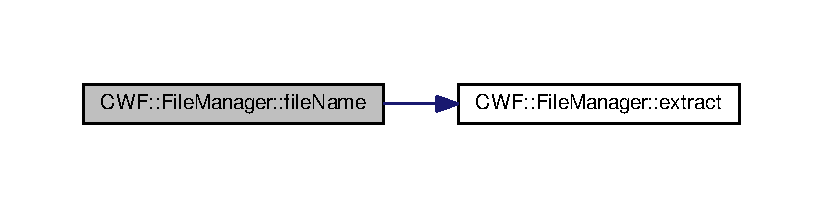
\includegraphics[width=350pt]{class_c_w_f_1_1_file_manager_a435ffe313b96261567da05806d38bacc_cgraph}
\end{center}
\end{figure}




Here is the caller graph for this function\+:
\nopagebreak
\begin{figure}[H]
\begin{center}
\leavevmode
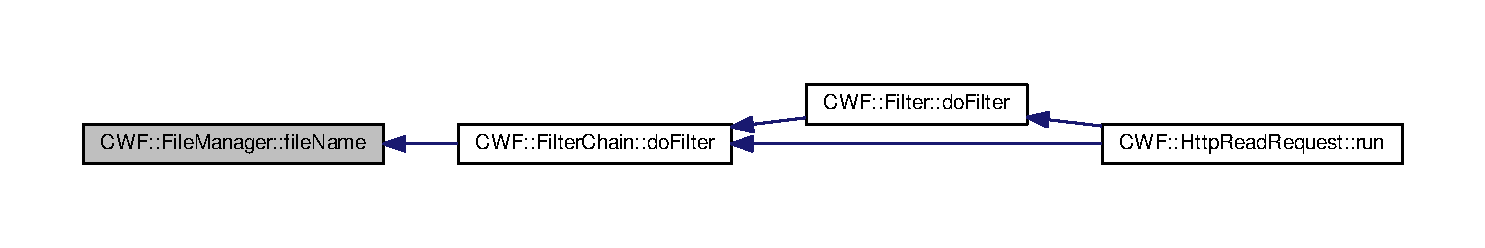
\includegraphics[width=350pt]{class_c_w_f_1_1_file_manager_a435ffe313b96261567da05806d38bacc_icgraph}
\end{center}
\end{figure}


\hypertarget{class_c_w_f_1_1_file_manager_af1c46c869cd3eece80c937556ecef9c8}{\index{C\+W\+F\+::\+File\+Manager@{C\+W\+F\+::\+File\+Manager}!put\+First\+Bar@{put\+First\+Bar}}
\index{put\+First\+Bar@{put\+First\+Bar}!C\+W\+F\+::\+File\+Manager@{C\+W\+F\+::\+File\+Manager}}
\subsubsection[{put\+First\+Bar}]{\setlength{\rightskip}{0pt plus 5cm}void C\+W\+F\+::\+File\+Manager\+::put\+First\+Bar (
\begin{DoxyParamCaption}
\item[{Q\+String \&}]{path}
\end{DoxyParamCaption}
) const}}\label{class_c_w_f_1_1_file_manager_af1c46c869cd3eece80c937556ecef9c8}
\hypertarget{class_c_w_f_1_1_file_manager_ad0e948a2e72ffa137027a3daa6055747}{\index{C\+W\+F\+::\+File\+Manager@{C\+W\+F\+::\+File\+Manager}!read\+All@{read\+All}}
\index{read\+All@{read\+All}!C\+W\+F\+::\+File\+Manager@{C\+W\+F\+::\+File\+Manager}}
\subsubsection[{read\+All}]{\setlength{\rightskip}{0pt plus 5cm}Q\+Byte\+Array C\+W\+F\+::\+File\+Manager\+::read\+All (
\begin{DoxyParamCaption}
\item[{const Q\+String \&}]{file\+Name, }
\item[{Q\+File\+Device\+::\+File\+Error \&}]{file\+Erro}
\end{DoxyParamCaption}
) const}}\label{class_c_w_f_1_1_file_manager_ad0e948a2e72ffa137027a3daa6055747}
\hypertarget{class_c_w_f_1_1_file_manager_aa7918801a52bd8789239542b1c368889}{\index{C\+W\+F\+::\+File\+Manager@{C\+W\+F\+::\+File\+Manager}!remove\+First\+Bar@{remove\+First\+Bar}}
\index{remove\+First\+Bar@{remove\+First\+Bar}!C\+W\+F\+::\+File\+Manager@{C\+W\+F\+::\+File\+Manager}}
\subsubsection[{remove\+First\+Bar}]{\setlength{\rightskip}{0pt plus 5cm}void C\+W\+F\+::\+File\+Manager\+::remove\+First\+Bar (
\begin{DoxyParamCaption}
\item[{Q\+String \&}]{path}
\end{DoxyParamCaption}
) const}}\label{class_c_w_f_1_1_file_manager_aa7918801a52bd8789239542b1c368889}


Here is the caller graph for this function\+:
\nopagebreak
\begin{figure}[H]
\begin{center}
\leavevmode
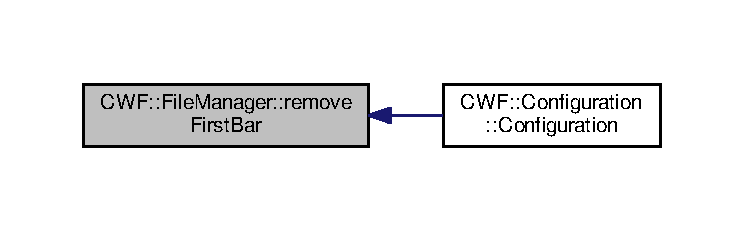
\includegraphics[width=350pt]{class_c_w_f_1_1_file_manager_aa7918801a52bd8789239542b1c368889_icgraph}
\end{center}
\end{figure}


\hypertarget{class_c_w_f_1_1_file_manager_a0b00584a292008515b686c67187bac13}{\index{C\+W\+F\+::\+File\+Manager@{C\+W\+F\+::\+File\+Manager}!remove\+Last\+Bar@{remove\+Last\+Bar}}
\index{remove\+Last\+Bar@{remove\+Last\+Bar}!C\+W\+F\+::\+File\+Manager@{C\+W\+F\+::\+File\+Manager}}
\subsubsection[{remove\+Last\+Bar}]{\setlength{\rightskip}{0pt plus 5cm}void C\+W\+F\+::\+File\+Manager\+::remove\+Last\+Bar (
\begin{DoxyParamCaption}
\item[{Q\+String \&}]{path}
\end{DoxyParamCaption}
) const}}\label{class_c_w_f_1_1_file_manager_a0b00584a292008515b686c67187bac13}


Here is the caller graph for this function\+:
\nopagebreak
\begin{figure}[H]
\begin{center}
\leavevmode
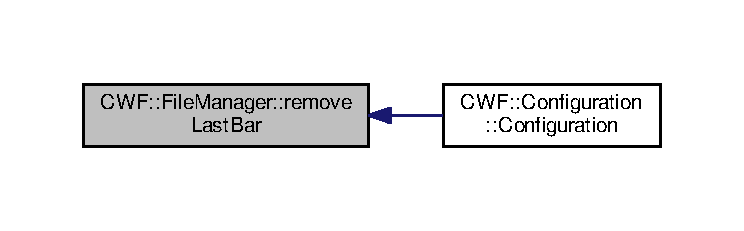
\includegraphics[width=350pt]{class_c_w_f_1_1_file_manager_a0b00584a292008515b686c67187bac13_icgraph}
\end{center}
\end{figure}




The documentation for this class was generated from the following files\+:\begin{DoxyCompactItemize}
\item 
/home/herik/\+C\+P\+P\+Web\+Framework/\+C\+P\+P\+Web\+Framework/cwf/\hyperlink{filemanager_8h}{filemanager.\+h}\item 
/home/herik/\+C\+P\+P\+Web\+Framework/\+C\+P\+P\+Web\+Framework/cwf/\hyperlink{filemanager_8cpp}{filemanager.\+cpp}\end{DoxyCompactItemize}

\hypertarget{class_c_w_f_1_1_filter}{\section{C\+W\+F\+:\+:Filter Class Reference}
\label{class_c_w_f_1_1_filter}\index{C\+W\+F\+::\+Filter@{C\+W\+F\+::\+Filter}}
}


The \hyperlink{class_c_w_f_1_1_filter}{Filter} class works like a filter. You can use this class to validate sessions or measuring runtime of a specific method, for example. To use this class, you will need to create a derived class and reconstruct the do\+Filter method, after this, you will need to configure it into the Configure\+Cpp\+Web\+Server, using the set\+Filter method.  




{\ttfamily \#include $<$filter.\+h$>$}

\subsection*{Public Member Functions}
\begin{DoxyCompactItemize}
\item 
virtual \hyperlink{class_c_w_f_1_1_filter_aa0ba072123bbcd95de94ff17d65e35aa}{$\sim$\+Filter} ()
\begin{DoxyCompactList}\small\item\em Virtual destructor. \end{DoxyCompactList}\item 
virtual void \hyperlink{class_c_w_f_1_1_filter_aa66add142c4f09a0b26f8d97a59650ba}{do\+Filter} (\hyperlink{class_c_w_f_1_1_http_servlet_request}{C\+W\+F\+::\+Http\+Servlet\+Request} \&request, \hyperlink{class_c_w_f_1_1_http_servlet_response}{C\+W\+F\+::\+Http\+Servlet\+Response} \&response, \hyperlink{class_c_w_f_1_1_filter_chain}{Filter\+Chain} \&chain)
\begin{DoxyCompactList}\small\item\em This method will be called always that the \hyperlink{class_c_w_f_1_1_cpp_web_server}{Cpp\+Web\+Server} receives a requisition. \end{DoxyCompactList}\end{DoxyCompactItemize}


\subsection{Detailed Description}
The \hyperlink{class_c_w_f_1_1_filter}{Filter} class works like a filter. You can use this class to validate sessions or measuring runtime of a specific method, for example. To use this class, you will need to create a derived class and reconstruct the do\+Filter method, after this, you will need to configure it into the Configure\+Cpp\+Web\+Server, using the set\+Filter method. 

\subsection{Constructor \& Destructor Documentation}
\hypertarget{class_c_w_f_1_1_filter_aa0ba072123bbcd95de94ff17d65e35aa}{\index{C\+W\+F\+::\+Filter@{C\+W\+F\+::\+Filter}!````~Filter@{$\sim$\+Filter}}
\index{````~Filter@{$\sim$\+Filter}!C\+W\+F\+::\+Filter@{C\+W\+F\+::\+Filter}}
\subsubsection[{$\sim$\+Filter}]{\setlength{\rightskip}{0pt plus 5cm}C\+W\+F\+::\+Filter\+::$\sim$\+Filter (
\begin{DoxyParamCaption}
{}
\end{DoxyParamCaption}
)\hspace{0.3cm}{\ttfamily [virtual]}}}\label{class_c_w_f_1_1_filter_aa0ba072123bbcd95de94ff17d65e35aa}


Virtual destructor. 



\subsection{Member Function Documentation}
\hypertarget{class_c_w_f_1_1_filter_aa66add142c4f09a0b26f8d97a59650ba}{\index{C\+W\+F\+::\+Filter@{C\+W\+F\+::\+Filter}!do\+Filter@{do\+Filter}}
\index{do\+Filter@{do\+Filter}!C\+W\+F\+::\+Filter@{C\+W\+F\+::\+Filter}}
\subsubsection[{do\+Filter}]{\setlength{\rightskip}{0pt plus 5cm}void C\+W\+F\+::\+Filter\+::do\+Filter (
\begin{DoxyParamCaption}
\item[{{\bf C\+W\+F\+::\+Http\+Servlet\+Request} \&}]{request, }
\item[{{\bf C\+W\+F\+::\+Http\+Servlet\+Response} \&}]{response, }
\item[{{\bf Filter\+Chain} \&}]{chain}
\end{DoxyParamCaption}
)\hspace{0.3cm}{\ttfamily [virtual]}}}\label{class_c_w_f_1_1_filter_aa66add142c4f09a0b26f8d97a59650ba}


This method will be called always that the \hyperlink{class_c_w_f_1_1_cpp_web_server}{Cpp\+Web\+Server} receives a requisition. 


\begin{DoxyParams}{Parameters}
{\em request} & \+: This is a reference to the \hyperlink{class_c_w_f_1_1_http_servlet_request}{Http\+Servlet\+Request}. \\
\hline
{\em response} & \+: This is a reference to the \hyperlink{class_c_w_f_1_1_http_servlet_response}{Http\+Servlet\+Response}. \\
\hline
{\em chain} & \+: This is a reference to the \hyperlink{class_c_w_f_1_1_filter_chain}{Filter\+Chain}. \\
\hline
\end{DoxyParams}
\begin{DoxyParagraph}{Example}

\begin{DoxyCode}
\textcolor{comment}{//----loginfilter.h-----}

\textcolor{preprocessor}{#ifndef LOGINFILTER\_H}
\textcolor{preprocessor}{#define LOGINFILTER\_H}

\textcolor{preprocessor}{#include "\hyperlink{filter_8h}{cwf/filter.h}"}

\textcolor{keyword}{class }LoginFilter : \textcolor{keyword}{public} \hyperlink{class_c_w_f_1_1_filter}{CWF::Filter}
\{
\textcolor{keyword}{public}:
    \textcolor{keywordtype}{void} \hyperlink{class_c_w_f_1_1_filter_aa66add142c4f09a0b26f8d97a59650ba}{doFilter}(\hyperlink{class_c_w_f_1_1_http_servlet_request}{CWF::HttpServletRequest} &request, 
      \hyperlink{class_c_w_f_1_1_http_servlet_response}{CWF::HttpServletResponse} &response, \hyperlink{class_c_w_f_1_1_filter_chain}{CWF::FilterChain} &chain)
    \{
        QString url = request.\hyperlink{class_c_w_f_1_1_http_servlet_request_a9408f2866aa0fc49242e74b85a514869}{getRequestURL}();
        \textcolor{keywordflow}{if}(url.endsWith(\textcolor{stringliteral}{".css"}) || url.endsWith(\textcolor{stringliteral}{".png"}) || url.endsWith(\textcolor{stringliteral}{".jpg"}))
        \{
            chain.\hyperlink{class_c_w_f_1_1_filter_chain_a438bc63ea1fa575ae8882fb05a31feca}{doFilter}(request, response);
        \}
        \textcolor{keywordflow}{else} \textcolor{keywordflow}{if}(url != \textcolor{stringliteral}{"/login"})
        \{
            \textcolor{keywordflow}{if}(request.\hyperlink{class_c_w_f_1_1_http_servlet_request_aad0cadb7d24101705a6f83b82eb7c025}{getSession}().\hyperlink{class_c_w_f_1_1_http_session_a44f59df340395d9c298c93ee5307b392}{getAttribute}(\textcolor{stringliteral}{"user"}) == \textcolor{keyword}{nullptr} || request.
      \hyperlink{class_c_w_f_1_1_http_servlet_request_aad0cadb7d24101705a6f83b82eb7c025}{getSession}().\hyperlink{class_c_w_f_1_1_http_session_aebc716e79896ed61527ff4dac933558e}{isExpired}())
            \{
                request.\hyperlink{class_c_w_f_1_1_http_servlet_request_a0ce93d793a178c7e0e5fef4044b48bdc}{getRequestDispatcher}(\textcolor{stringliteral}{"/pages/login"}).
      \hyperlink{class_c_w_f_1_1_request_dispatcher_a075c11ff233f217196764899f9edf7d0}{forward}(request, response);
            \}
            \textcolor{keywordflow}{else}
            \{
                chain.\hyperlink{class_c_w_f_1_1_filter_chain_a438bc63ea1fa575ae8882fb05a31feca}{doFilter}(request, response);
            \}
         \}
         \textcolor{keywordflow}{else}
         \{
             chain.\hyperlink{class_c_w_f_1_1_filter_chain_a438bc63ea1fa575ae8882fb05a31feca}{doFilter}(request, response);
         \}
    \}
\};

\textcolor{preprocessor}{#endif // LOGINFILTER\_H}

\textcolor{comment}{//----main.h-----}

\textcolor{preprocessor}{#include <filter/loginfilter.h>}
\textcolor{preprocessor}{#include "\hyperlink{cppwebapplication_8h}{cwf/cppwebapplication.h}"}

\textcolor{keywordtype}{int} main(\textcolor{keywordtype}{int} argc, \textcolor{keywordtype}{char} *argv[])
\{
    \hyperlink{class_c_w_f_1_1_cpp_web_application}{CWF::CppWebApplication} server(argc,
                                  argv,
                                  \hyperlink{class_c_w_f_1_1_configuration}{CWF::Configuration}(\textcolor{stringliteral}{"
      /home/herik/CPPWebFramework/examples/Filters/server"}),
                                  \textcolor{keyword}{new} LoginFilter);

    \textcolor{keywordflow}{return} server.start();
\}
\end{DoxyCode}
 
\end{DoxyParagraph}


The documentation for this class was generated from the following files\+:\begin{DoxyCompactItemize}
\item 
/home/herik/\+C\+P\+P\+Web\+Framework/\+C\+P\+P\+Web\+Framework/cwf/\hyperlink{filter_8h}{filter.\+h}\item 
/home/herik/\+C\+P\+P\+Web\+Framework/\+C\+P\+P\+Web\+Framework/cwf/\hyperlink{filter_8cpp}{filter.\+cpp}\end{DoxyCompactItemize}

\hypertarget{class_c_w_f_1_1_filter_chain}{\section{C\+W\+F\+:\+:Filter\+Chain Class Reference}
\label{class_c_w_f_1_1_filter_chain}\index{C\+W\+F\+::\+Filter\+Chain@{C\+W\+F\+::\+Filter\+Chain}}
}


The \hyperlink{class_c_w_f_1_1_filter_chain}{Filter\+Chain} class is responsable to dispatch a requisition. This class was built to work with \hyperlink{class_c_w_f_1_1_filter}{Filter}. Always when a \hyperlink{class_c_w_f_1_1_filter}{Filter} makes all the necessary validations, it can dispatches the requisition to the \hyperlink{class_c_w_f_1_1_filter_chain}{Filter\+Chain}. N\+O\+T\+E\+: It is a final class, you can't derive from it.  




{\ttfamily \#include $<$filterchain.\+h$>$}

\subsection*{Public Member Functions}
\begin{DoxyCompactItemize}
\item 
\hyperlink{class_c_w_f_1_1_filter_chain_a2c108c6b3b588997381b6d861f2dd8b9}{Filter\+Chain} (\hyperlink{class_c_w_f_1_1_http_servlet}{Http\+Servlet} $\ast$servlet)
\begin{DoxyCompactList}\small\item\em \hyperlink{class_c_w_f_1_1_filter_chain}{Filter\+Chain}. \end{DoxyCompactList}\item 
void \hyperlink{class_c_w_f_1_1_filter_chain_a438bc63ea1fa575ae8882fb05a31feca}{do\+Filter} (\hyperlink{class_c_w_f_1_1_http_servlet_request}{C\+W\+F\+::\+Http\+Servlet\+Request} \&request, \hyperlink{class_c_w_f_1_1_http_servlet_response}{C\+W\+F\+::\+Http\+Servlet\+Response} \&response)
\begin{DoxyCompactList}\small\item\em This method dispaches a requisition to a \hyperlink{class_c_w_f_1_1_http_servlet_request}{Http\+Servlet\+Request} or, if the requesition is for a file, it can reads and send the file through the \hyperlink{class_c_w_f_1_1_http_servlet_response}{Http\+Servlet\+Response}. \end{DoxyCompactList}\end{DoxyCompactItemize}


\subsection{Detailed Description}
The \hyperlink{class_c_w_f_1_1_filter_chain}{Filter\+Chain} class is responsable to dispatch a requisition. This class was built to work with \hyperlink{class_c_w_f_1_1_filter}{Filter}. Always when a \hyperlink{class_c_w_f_1_1_filter}{Filter} makes all the necessary validations, it can dispatches the requisition to the \hyperlink{class_c_w_f_1_1_filter_chain}{Filter\+Chain}. N\+O\+T\+E\+: It is a final class, you can't derive from it. 

\subsection{Constructor \& Destructor Documentation}
\hypertarget{class_c_w_f_1_1_filter_chain_a2c108c6b3b588997381b6d861f2dd8b9}{\index{C\+W\+F\+::\+Filter\+Chain@{C\+W\+F\+::\+Filter\+Chain}!Filter\+Chain@{Filter\+Chain}}
\index{Filter\+Chain@{Filter\+Chain}!C\+W\+F\+::\+Filter\+Chain@{C\+W\+F\+::\+Filter\+Chain}}
\subsubsection[{Filter\+Chain}]{\setlength{\rightskip}{0pt plus 5cm}C\+W\+F\+::\+Filter\+Chain\+::\+Filter\+Chain (
\begin{DoxyParamCaption}
\item[{{\bf Http\+Servlet} $\ast$}]{servlet}
\end{DoxyParamCaption}
)}}\label{class_c_w_f_1_1_filter_chain_a2c108c6b3b588997381b6d861f2dd8b9}


\hyperlink{class_c_w_f_1_1_filter_chain}{Filter\+Chain}. 


\begin{DoxyParams}{Parameters}
{\em servlet} & \\
\hline
\end{DoxyParams}


\subsection{Member Function Documentation}
\hypertarget{class_c_w_f_1_1_filter_chain_a438bc63ea1fa575ae8882fb05a31feca}{\index{C\+W\+F\+::\+Filter\+Chain@{C\+W\+F\+::\+Filter\+Chain}!do\+Filter@{do\+Filter}}
\index{do\+Filter@{do\+Filter}!C\+W\+F\+::\+Filter\+Chain@{C\+W\+F\+::\+Filter\+Chain}}
\subsubsection[{do\+Filter}]{\setlength{\rightskip}{0pt plus 5cm}void C\+W\+F\+::\+Filter\+Chain\+::do\+Filter (
\begin{DoxyParamCaption}
\item[{{\bf C\+W\+F\+::\+Http\+Servlet\+Request} \&}]{request, }
\item[{{\bf C\+W\+F\+::\+Http\+Servlet\+Response} \&}]{response}
\end{DoxyParamCaption}
)}}\label{class_c_w_f_1_1_filter_chain_a438bc63ea1fa575ae8882fb05a31feca}


This method dispaches a requisition to a \hyperlink{class_c_w_f_1_1_http_servlet_request}{Http\+Servlet\+Request} or, if the requesition is for a file, it can reads and send the file through the \hyperlink{class_c_w_f_1_1_http_servlet_response}{Http\+Servlet\+Response}. 


\begin{DoxyParams}{Parameters}
{\em request} & \+: This is a reference to the \hyperlink{class_c_w_f_1_1_http_servlet_request}{Http\+Servlet\+Request}. \\
\hline
{\em response} & \+: This is a reference to the \hyperlink{class_c_w_f_1_1_http_servlet_response}{Http\+Servlet\+Response}. \\
\hline
\end{DoxyParams}


Here is the call graph for this function\+:
\nopagebreak
\begin{figure}[H]
\begin{center}
\leavevmode
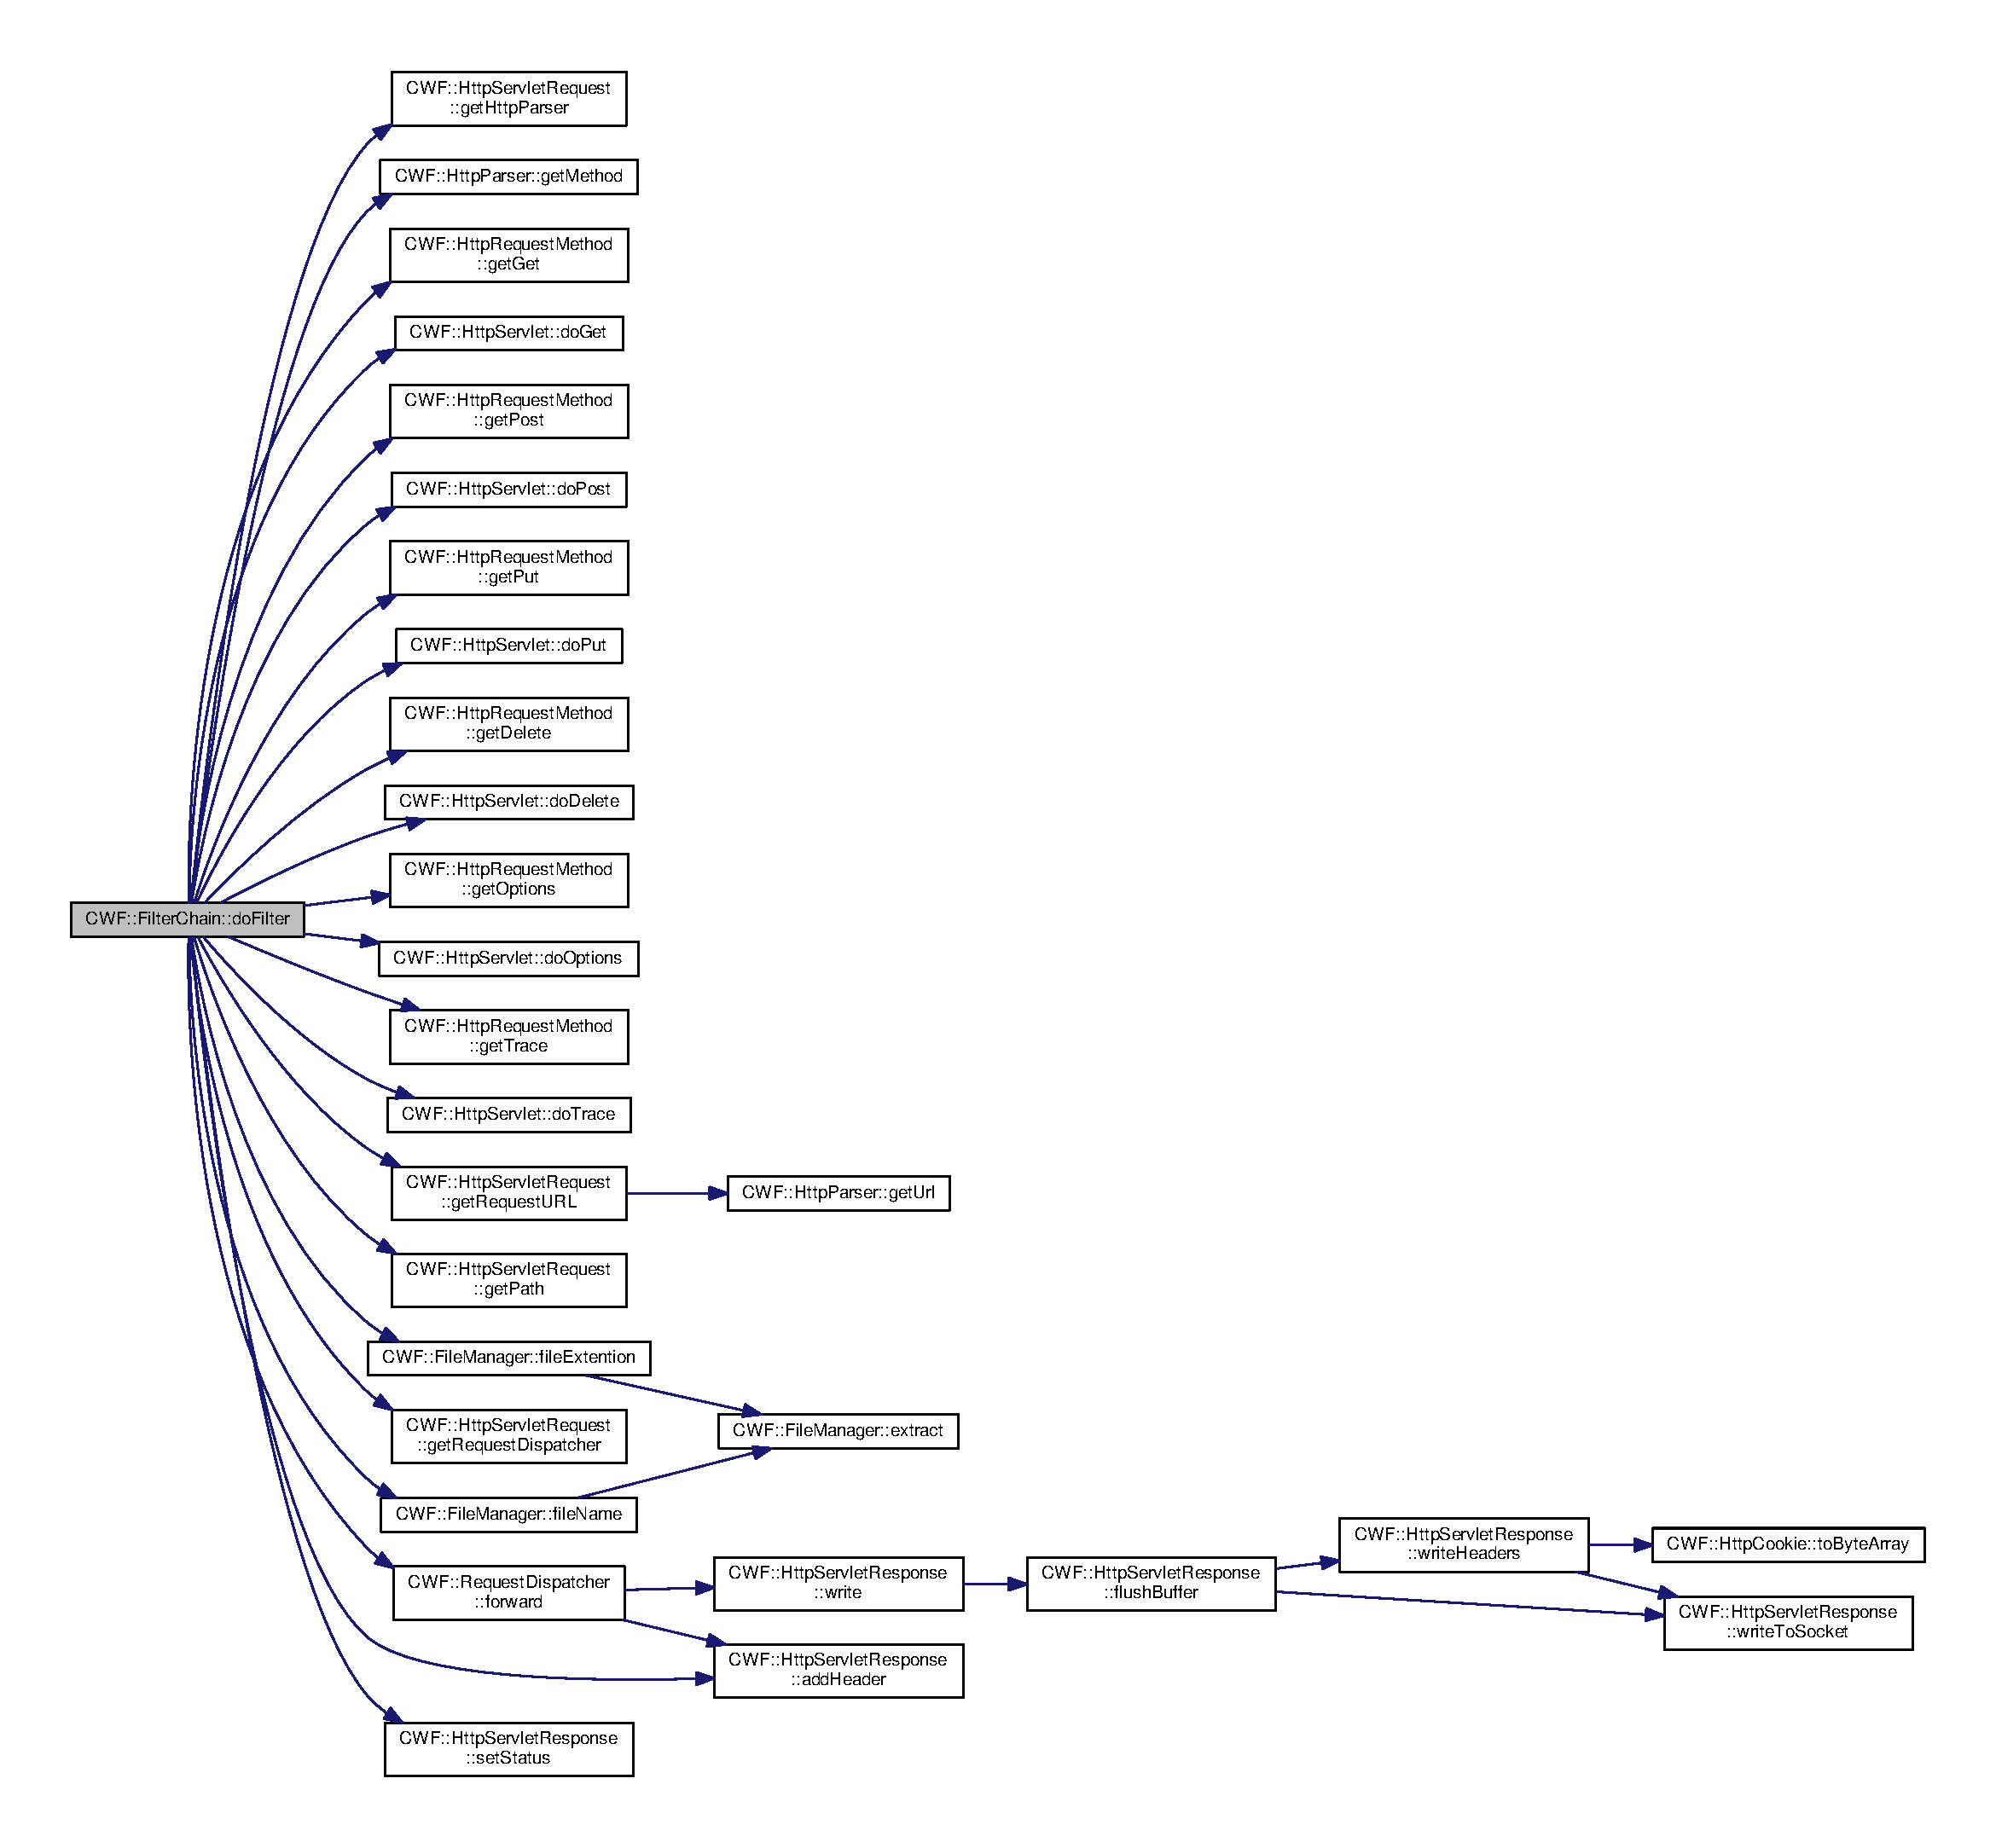
\includegraphics[width=350pt]{class_c_w_f_1_1_filter_chain_a438bc63ea1fa575ae8882fb05a31feca_cgraph}
\end{center}
\end{figure}




Here is the caller graph for this function\+:
\nopagebreak
\begin{figure}[H]
\begin{center}
\leavevmode
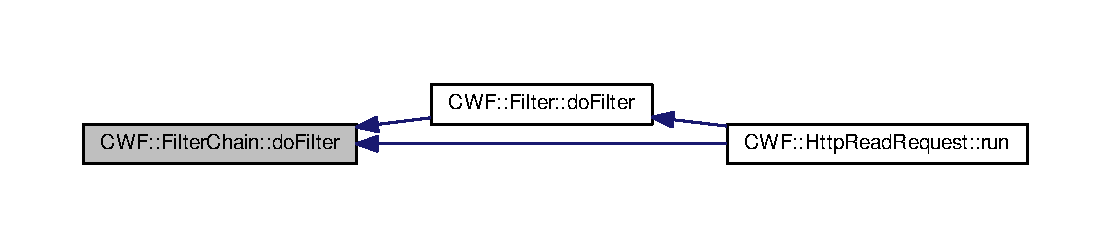
\includegraphics[width=350pt]{class_c_w_f_1_1_filter_chain_a438bc63ea1fa575ae8882fb05a31feca_icgraph}
\end{center}
\end{figure}




The documentation for this class was generated from the following files\+:\begin{DoxyCompactItemize}
\item 
/home/herik/\+C\+P\+P\+Web\+Framework/\+C\+P\+P\+Web\+Framework/cwf/\hyperlink{filterchain_8h}{filterchain.\+h}\item 
/home/herik/\+C\+P\+P\+Web\+Framework/\+C\+P\+P\+Web\+Framework/cwf/\hyperlink{filterchain_8cpp}{filterchain.\+cpp}\end{DoxyCompactItemize}

\hypertarget{class_c_w_f_1_1_for_attributes}{\section{C\+W\+F\+:\+:For\+Attributes Class Reference}
\label{class_c_w_f_1_1_for_attributes}\index{C\+W\+F\+::\+For\+Attributes@{C\+W\+F\+::\+For\+Attributes}}
}


The \hyperlink{class_c_w_f_1_1_for_attributes}{For\+Attributes} class is an auxiliar class to the \hyperlink{class_c_w_f_1_1_c_s_t_l_compiler}{C\+S\+T\+L\+Compiler}.  




{\ttfamily \#include $<$forattributes.\+h$>$}

\subsection*{Public Member Functions}
\begin{DoxyCompactItemize}
\item 
\hyperlink{class_c_w_f_1_1_for_attributes_a8b2245bb0b5b8b16de346ac8402678a0}{For\+Attributes} (const Q\+Xml\+Stream\+Attributes \&attributes)
\end{DoxyCompactItemize}
\subsection*{Public Attributes}
\begin{DoxyCompactItemize}
\item 
Q\+String \hyperlink{class_c_w_f_1_1_for_attributes_a531689e9e92369507be81971caf347a6}{var}
\item 
Q\+String \hyperlink{class_c_w_f_1_1_for_attributes_aa16fb4090c8e95ec98f8f9a1ff768dd3}{items}
\item 
Q\+String \hyperlink{class_c_w_f_1_1_for_attributes_ac27ba2f6562de074fb345d577f171ad6}{error}
\item 
Q\+String \hyperlink{class_c_w_f_1_1_for_attributes_acb6db58dc865974f20f1b9a291f7a94b}{from}
\item 
Q\+String \hyperlink{class_c_w_f_1_1_for_attributes_a33cef70ab52e64d4157ad75c8bfe604a}{to}
\item 
Q\+String \hyperlink{class_c_w_f_1_1_for_attributes_a316811830dab52e5f38eb8a5f43f1164}{increment}
\end{DoxyCompactItemize}


\subsection{Detailed Description}
The \hyperlink{class_c_w_f_1_1_for_attributes}{For\+Attributes} class is an auxiliar class to the \hyperlink{class_c_w_f_1_1_c_s_t_l_compiler}{C\+S\+T\+L\+Compiler}. 

\subsection{Constructor \& Destructor Documentation}
\hypertarget{class_c_w_f_1_1_for_attributes_a8b2245bb0b5b8b16de346ac8402678a0}{\index{C\+W\+F\+::\+For\+Attributes@{C\+W\+F\+::\+For\+Attributes}!For\+Attributes@{For\+Attributes}}
\index{For\+Attributes@{For\+Attributes}!C\+W\+F\+::\+For\+Attributes@{C\+W\+F\+::\+For\+Attributes}}
\subsubsection[{For\+Attributes}]{\setlength{\rightskip}{0pt plus 5cm}C\+W\+F\+::\+For\+Attributes\+::\+For\+Attributes (
\begin{DoxyParamCaption}
\item[{const Q\+Xml\+Stream\+Attributes \&}]{attributes}
\end{DoxyParamCaption}
)}}\label{class_c_w_f_1_1_for_attributes_a8b2245bb0b5b8b16de346ac8402678a0}


\subsection{Member Data Documentation}
\hypertarget{class_c_w_f_1_1_for_attributes_ac27ba2f6562de074fb345d577f171ad6}{\index{C\+W\+F\+::\+For\+Attributes@{C\+W\+F\+::\+For\+Attributes}!error@{error}}
\index{error@{error}!C\+W\+F\+::\+For\+Attributes@{C\+W\+F\+::\+For\+Attributes}}
\subsubsection[{error}]{\setlength{\rightskip}{0pt plus 5cm}Q\+String C\+W\+F\+::\+For\+Attributes\+::error}}\label{class_c_w_f_1_1_for_attributes_ac27ba2f6562de074fb345d577f171ad6}
\hypertarget{class_c_w_f_1_1_for_attributes_acb6db58dc865974f20f1b9a291f7a94b}{\index{C\+W\+F\+::\+For\+Attributes@{C\+W\+F\+::\+For\+Attributes}!from@{from}}
\index{from@{from}!C\+W\+F\+::\+For\+Attributes@{C\+W\+F\+::\+For\+Attributes}}
\subsubsection[{from}]{\setlength{\rightskip}{0pt plus 5cm}Q\+String C\+W\+F\+::\+For\+Attributes\+::from}}\label{class_c_w_f_1_1_for_attributes_acb6db58dc865974f20f1b9a291f7a94b}
\hypertarget{class_c_w_f_1_1_for_attributes_a316811830dab52e5f38eb8a5f43f1164}{\index{C\+W\+F\+::\+For\+Attributes@{C\+W\+F\+::\+For\+Attributes}!increment@{increment}}
\index{increment@{increment}!C\+W\+F\+::\+For\+Attributes@{C\+W\+F\+::\+For\+Attributes}}
\subsubsection[{increment}]{\setlength{\rightskip}{0pt plus 5cm}Q\+String C\+W\+F\+::\+For\+Attributes\+::increment}}\label{class_c_w_f_1_1_for_attributes_a316811830dab52e5f38eb8a5f43f1164}
\hypertarget{class_c_w_f_1_1_for_attributes_aa16fb4090c8e95ec98f8f9a1ff768dd3}{\index{C\+W\+F\+::\+For\+Attributes@{C\+W\+F\+::\+For\+Attributes}!items@{items}}
\index{items@{items}!C\+W\+F\+::\+For\+Attributes@{C\+W\+F\+::\+For\+Attributes}}
\subsubsection[{items}]{\setlength{\rightskip}{0pt plus 5cm}Q\+String C\+W\+F\+::\+For\+Attributes\+::items}}\label{class_c_w_f_1_1_for_attributes_aa16fb4090c8e95ec98f8f9a1ff768dd3}
\hypertarget{class_c_w_f_1_1_for_attributes_a33cef70ab52e64d4157ad75c8bfe604a}{\index{C\+W\+F\+::\+For\+Attributes@{C\+W\+F\+::\+For\+Attributes}!to@{to}}
\index{to@{to}!C\+W\+F\+::\+For\+Attributes@{C\+W\+F\+::\+For\+Attributes}}
\subsubsection[{to}]{\setlength{\rightskip}{0pt plus 5cm}Q\+String C\+W\+F\+::\+For\+Attributes\+::to}}\label{class_c_w_f_1_1_for_attributes_a33cef70ab52e64d4157ad75c8bfe604a}
\hypertarget{class_c_w_f_1_1_for_attributes_a531689e9e92369507be81971caf347a6}{\index{C\+W\+F\+::\+For\+Attributes@{C\+W\+F\+::\+For\+Attributes}!var@{var}}
\index{var@{var}!C\+W\+F\+::\+For\+Attributes@{C\+W\+F\+::\+For\+Attributes}}
\subsubsection[{var}]{\setlength{\rightskip}{0pt plus 5cm}Q\+String C\+W\+F\+::\+For\+Attributes\+::var}}\label{class_c_w_f_1_1_for_attributes_a531689e9e92369507be81971caf347a6}


The documentation for this class was generated from the following files\+:\begin{DoxyCompactItemize}
\item 
/home/herik/\+C\+P\+P\+Web\+Framework/\+C\+P\+P\+Web\+Framework/cwf/\hyperlink{forattributes_8h}{forattributes.\+h}\item 
/home/herik/\+C\+P\+P\+Web\+Framework/\+C\+P\+P\+Web\+Framework/cwf/\hyperlink{forattributes_8cpp}{forattributes.\+cpp}\end{DoxyCompactItemize}

\hypertarget{class_c_w_f_1_1_http_cookie}{\section{C\+W\+F\+:\+:Http\+Cookie Class Reference}
\label{class_c_w_f_1_1_http_cookie}\index{C\+W\+F\+::\+Http\+Cookie@{C\+W\+F\+::\+Http\+Cookie}}
}


This class represents a H\+T\+T\+P Cookie.  




{\ttfamily \#include $<$httpcookie.\+h$>$}

\subsection*{Public Member Functions}
\begin{DoxyCompactItemize}
\item 
\hyperlink{class_c_w_f_1_1_http_cookie_a36fafa10bc6c2580acf0b11f007b11ae}{Http\+Cookie} ()=default
\begin{DoxyCompactList}\small\item\em This is the cookie's default constructor. \end{DoxyCompactList}\item 
\hyperlink{class_c_w_f_1_1_http_cookie_a8e43ce5eabd7a7e8dd375232ad3b568e}{Http\+Cookie} (const Q\+Byte\+Array \&source)
\item 
\hyperlink{class_c_w_f_1_1_http_cookie_a2429ad80884ddb6712a9f1fa98e03eac}{Http\+Cookie} (const Q\+Byte\+Array \&name, const Q\+Byte\+Array \&value)
\begin{DoxyCompactList}\small\item\em This is an overloaded constructor that receives a cookie's name and value. \end{DoxyCompactList}\item 
Q\+Byte\+Array \hyperlink{class_c_w_f_1_1_http_cookie_a84c6628ab6c1955fe784bfbe6e66ca7e}{to\+Byte\+Array} () const 
\item 
void \hyperlink{class_c_w_f_1_1_http_cookie_a03cae390cca7717a71ee00d06c8ae8a5}{set\+Name} (const Q\+Byte\+Array \&name)
\item 
void \hyperlink{class_c_w_f_1_1_http_cookie_a0922f5fcdf3873a24ec9a323f10e5a40}{set\+Value} (const Q\+Byte\+Array \&value)
\item 
void \hyperlink{class_c_w_f_1_1_http_cookie_a387cf2fbe8bc9eaeac96f1c5b7ee39a2}{set\+Comment} (const Q\+Byte\+Array \&comment)
\item 
void \hyperlink{class_c_w_f_1_1_http_cookie_a74edb046a8816680bb53a1574b1e1d13}{set\+Domain} (const Q\+Byte\+Array \&domain)
\item 
void \hyperlink{class_c_w_f_1_1_http_cookie_ad3ba0b75ebaeddaa893b82446d8a4459}{set\+Max\+Age} (int max\+Age)
\item 
void \hyperlink{class_c_w_f_1_1_http_cookie_ab9a831a7cb2e46db2be96a947f259ad5}{set\+Path} (const Q\+Byte\+Array \&path)
\item 
void \hyperlink{class_c_w_f_1_1_http_cookie_aee31add3a00be4de84620c191f61457e}{set\+Secure} (bool secure)
\item 
Q\+Byte\+Array \hyperlink{class_c_w_f_1_1_http_cookie_a7e0e3d818e1abb1a87c27ad64d3ef1bd}{get\+Name} () const 
\item 
Q\+Byte\+Array \hyperlink{class_c_w_f_1_1_http_cookie_a6dfaa65b0fdc459987adffbb9957eb89}{get\+Value} () const 
\item 
Q\+Byte\+Array \hyperlink{class_c_w_f_1_1_http_cookie_a6cb9c628c0c9eb714945dc9227a85c03}{get\+Comment} () const 
\item 
Q\+Byte\+Array \hyperlink{class_c_w_f_1_1_http_cookie_ad50d4e09e1f63daa18887e1d5349dc1e}{get\+Domain} () const 
\item 
int \hyperlink{class_c_w_f_1_1_http_cookie_ad1e15510ff41114f5d96d17e697b3911}{get\+Max\+Age} () const 
\item 
Q\+Byte\+Array \hyperlink{class_c_w_f_1_1_http_cookie_ad34b0b8cfd90ecc2bc612c6d13227ddc}{get\+Path} () const 
\item 
bool \hyperlink{class_c_w_f_1_1_http_cookie_a1d0917c49dcd958df946c680a8a555a2}{get\+Secure} () const 
\item 
int \hyperlink{class_c_w_f_1_1_http_cookie_a7b44ee026837508edd121caf5dfd205b}{get\+Version} () const 
\end{DoxyCompactItemize}
\subsection*{Static Public Member Functions}
\begin{DoxyCompactItemize}
\item 
static Q\+List$<$ Q\+Byte\+Array $>$ \hyperlink{class_c_w_f_1_1_http_cookie_aa36c86ebed49fe292745f2a3154d3c52}{split\+C\+S\+V} (const Q\+Byte\+Array \&source)
\end{DoxyCompactItemize}


\subsection{Detailed Description}
This class represents a H\+T\+T\+P Cookie. 

\subsection{Constructor \& Destructor Documentation}
\hypertarget{class_c_w_f_1_1_http_cookie_a36fafa10bc6c2580acf0b11f007b11ae}{\index{C\+W\+F\+::\+Http\+Cookie@{C\+W\+F\+::\+Http\+Cookie}!Http\+Cookie@{Http\+Cookie}}
\index{Http\+Cookie@{Http\+Cookie}!C\+W\+F\+::\+Http\+Cookie@{C\+W\+F\+::\+Http\+Cookie}}
\subsubsection[{Http\+Cookie}]{\setlength{\rightskip}{0pt plus 5cm}C\+W\+F\+::\+Http\+Cookie\+::\+Http\+Cookie (
\begin{DoxyParamCaption}
{}
\end{DoxyParamCaption}
)\hspace{0.3cm}{\ttfamily [default]}}}\label{class_c_w_f_1_1_http_cookie_a36fafa10bc6c2580acf0b11f007b11ae}


This is the cookie's default constructor. 

\hypertarget{class_c_w_f_1_1_http_cookie_a8e43ce5eabd7a7e8dd375232ad3b568e}{\index{C\+W\+F\+::\+Http\+Cookie@{C\+W\+F\+::\+Http\+Cookie}!Http\+Cookie@{Http\+Cookie}}
\index{Http\+Cookie@{Http\+Cookie}!C\+W\+F\+::\+Http\+Cookie@{C\+W\+F\+::\+Http\+Cookie}}
\subsubsection[{Http\+Cookie}]{\setlength{\rightskip}{0pt plus 5cm}C\+W\+F\+::\+Http\+Cookie\+::\+Http\+Cookie (
\begin{DoxyParamCaption}
\item[{const Q\+Byte\+Array \&}]{source}
\end{DoxyParamCaption}
)}}\label{class_c_w_f_1_1_http_cookie_a8e43ce5eabd7a7e8dd375232ad3b568e}
Create a cookie from a string. 
\begin{DoxyParams}{Parameters}
{\em source} & String as received in a H\+T\+T\+P Cookie2 header. \\
\hline
\end{DoxyParams}
\hypertarget{class_c_w_f_1_1_http_cookie_a2429ad80884ddb6712a9f1fa98e03eac}{\index{C\+W\+F\+::\+Http\+Cookie@{C\+W\+F\+::\+Http\+Cookie}!Http\+Cookie@{Http\+Cookie}}
\index{Http\+Cookie@{Http\+Cookie}!C\+W\+F\+::\+Http\+Cookie@{C\+W\+F\+::\+Http\+Cookie}}
\subsubsection[{Http\+Cookie}]{\setlength{\rightskip}{0pt plus 5cm}C\+W\+F\+::\+Http\+Cookie\+::\+Http\+Cookie (
\begin{DoxyParamCaption}
\item[{const Q\+Byte\+Array \&}]{name, }
\item[{const Q\+Byte\+Array \&}]{value}
\end{DoxyParamCaption}
)}}\label{class_c_w_f_1_1_http_cookie_a2429ad80884ddb6712a9f1fa98e03eac}


This is an overloaded constructor that receives a cookie's name and value. 


\begin{DoxyParams}{Parameters}
{\em name} & \+: This is a reference to a Q\+Byte\+Array. It will change the cookie's name. \\
\hline
{\em value} & \+: This is a reference to a Q\+Byte\+Array. It will change the cookie's value. \\
\hline
\end{DoxyParams}


\subsection{Member Function Documentation}
\hypertarget{class_c_w_f_1_1_http_cookie_a6cb9c628c0c9eb714945dc9227a85c03}{\index{C\+W\+F\+::\+Http\+Cookie@{C\+W\+F\+::\+Http\+Cookie}!get\+Comment@{get\+Comment}}
\index{get\+Comment@{get\+Comment}!C\+W\+F\+::\+Http\+Cookie@{C\+W\+F\+::\+Http\+Cookie}}
\subsubsection[{get\+Comment}]{\setlength{\rightskip}{0pt plus 5cm}Q\+Byte\+Array C\+W\+F\+::\+Http\+Cookie\+::get\+Comment (
\begin{DoxyParamCaption}
{}
\end{DoxyParamCaption}
) const}}\label{class_c_w_f_1_1_http_cookie_a6cb9c628c0c9eb714945dc9227a85c03}
Get the comment of this cookie \hypertarget{class_c_w_f_1_1_http_cookie_ad50d4e09e1f63daa18887e1d5349dc1e}{\index{C\+W\+F\+::\+Http\+Cookie@{C\+W\+F\+::\+Http\+Cookie}!get\+Domain@{get\+Domain}}
\index{get\+Domain@{get\+Domain}!C\+W\+F\+::\+Http\+Cookie@{C\+W\+F\+::\+Http\+Cookie}}
\subsubsection[{get\+Domain}]{\setlength{\rightskip}{0pt plus 5cm}Q\+Byte\+Array C\+W\+F\+::\+Http\+Cookie\+::get\+Domain (
\begin{DoxyParamCaption}
{}
\end{DoxyParamCaption}
) const}}\label{class_c_w_f_1_1_http_cookie_ad50d4e09e1f63daa18887e1d5349dc1e}
Get the domain of this cookie \hypertarget{class_c_w_f_1_1_http_cookie_ad1e15510ff41114f5d96d17e697b3911}{\index{C\+W\+F\+::\+Http\+Cookie@{C\+W\+F\+::\+Http\+Cookie}!get\+Max\+Age@{get\+Max\+Age}}
\index{get\+Max\+Age@{get\+Max\+Age}!C\+W\+F\+::\+Http\+Cookie@{C\+W\+F\+::\+Http\+Cookie}}
\subsubsection[{get\+Max\+Age}]{\setlength{\rightskip}{0pt plus 5cm}int C\+W\+F\+::\+Http\+Cookie\+::get\+Max\+Age (
\begin{DoxyParamCaption}
{}
\end{DoxyParamCaption}
) const}}\label{class_c_w_f_1_1_http_cookie_ad1e15510ff41114f5d96d17e697b3911}
Set the maximum age of this cookie in seconds. \hypertarget{class_c_w_f_1_1_http_cookie_a7e0e3d818e1abb1a87c27ad64d3ef1bd}{\index{C\+W\+F\+::\+Http\+Cookie@{C\+W\+F\+::\+Http\+Cookie}!get\+Name@{get\+Name}}
\index{get\+Name@{get\+Name}!C\+W\+F\+::\+Http\+Cookie@{C\+W\+F\+::\+Http\+Cookie}}
\subsubsection[{get\+Name}]{\setlength{\rightskip}{0pt plus 5cm}Q\+Byte\+Array C\+W\+F\+::\+Http\+Cookie\+::get\+Name (
\begin{DoxyParamCaption}
{}
\end{DoxyParamCaption}
) const}}\label{class_c_w_f_1_1_http_cookie_a7e0e3d818e1abb1a87c27ad64d3ef1bd}
Get the name of this cookie \hypertarget{class_c_w_f_1_1_http_cookie_ad34b0b8cfd90ecc2bc612c6d13227ddc}{\index{C\+W\+F\+::\+Http\+Cookie@{C\+W\+F\+::\+Http\+Cookie}!get\+Path@{get\+Path}}
\index{get\+Path@{get\+Path}!C\+W\+F\+::\+Http\+Cookie@{C\+W\+F\+::\+Http\+Cookie}}
\subsubsection[{get\+Path}]{\setlength{\rightskip}{0pt plus 5cm}Q\+Byte\+Array C\+W\+F\+::\+Http\+Cookie\+::get\+Path (
\begin{DoxyParamCaption}
{}
\end{DoxyParamCaption}
) const}}\label{class_c_w_f_1_1_http_cookie_ad34b0b8cfd90ecc2bc612c6d13227ddc}
Set the path of this cookie \hypertarget{class_c_w_f_1_1_http_cookie_a1d0917c49dcd958df946c680a8a555a2}{\index{C\+W\+F\+::\+Http\+Cookie@{C\+W\+F\+::\+Http\+Cookie}!get\+Secure@{get\+Secure}}
\index{get\+Secure@{get\+Secure}!C\+W\+F\+::\+Http\+Cookie@{C\+W\+F\+::\+Http\+Cookie}}
\subsubsection[{get\+Secure}]{\setlength{\rightskip}{0pt plus 5cm}bool C\+W\+F\+::\+Http\+Cookie\+::get\+Secure (
\begin{DoxyParamCaption}
{}
\end{DoxyParamCaption}
) const}}\label{class_c_w_f_1_1_http_cookie_a1d0917c49dcd958df946c680a8a555a2}
Get the secure flag of this cookie \hypertarget{class_c_w_f_1_1_http_cookie_a6dfaa65b0fdc459987adffbb9957eb89}{\index{C\+W\+F\+::\+Http\+Cookie@{C\+W\+F\+::\+Http\+Cookie}!get\+Value@{get\+Value}}
\index{get\+Value@{get\+Value}!C\+W\+F\+::\+Http\+Cookie@{C\+W\+F\+::\+Http\+Cookie}}
\subsubsection[{get\+Value}]{\setlength{\rightskip}{0pt plus 5cm}Q\+Byte\+Array C\+W\+F\+::\+Http\+Cookie\+::get\+Value (
\begin{DoxyParamCaption}
{}
\end{DoxyParamCaption}
) const}}\label{class_c_w_f_1_1_http_cookie_a6dfaa65b0fdc459987adffbb9957eb89}
Get the value of this cookie \hypertarget{class_c_w_f_1_1_http_cookie_a7b44ee026837508edd121caf5dfd205b}{\index{C\+W\+F\+::\+Http\+Cookie@{C\+W\+F\+::\+Http\+Cookie}!get\+Version@{get\+Version}}
\index{get\+Version@{get\+Version}!C\+W\+F\+::\+Http\+Cookie@{C\+W\+F\+::\+Http\+Cookie}}
\subsubsection[{get\+Version}]{\setlength{\rightskip}{0pt plus 5cm}int C\+W\+F\+::\+Http\+Cookie\+::get\+Version (
\begin{DoxyParamCaption}
{}
\end{DoxyParamCaption}
) const}}\label{class_c_w_f_1_1_http_cookie_a7b44ee026837508edd121caf5dfd205b}
Returns always 1 \hypertarget{class_c_w_f_1_1_http_cookie_a387cf2fbe8bc9eaeac96f1c5b7ee39a2}{\index{C\+W\+F\+::\+Http\+Cookie@{C\+W\+F\+::\+Http\+Cookie}!set\+Comment@{set\+Comment}}
\index{set\+Comment@{set\+Comment}!C\+W\+F\+::\+Http\+Cookie@{C\+W\+F\+::\+Http\+Cookie}}
\subsubsection[{set\+Comment}]{\setlength{\rightskip}{0pt plus 5cm}void C\+W\+F\+::\+Http\+Cookie\+::set\+Comment (
\begin{DoxyParamCaption}
\item[{const Q\+Byte\+Array \&}]{comment}
\end{DoxyParamCaption}
)}}\label{class_c_w_f_1_1_http_cookie_a387cf2fbe8bc9eaeac96f1c5b7ee39a2}
Set the comment of this cookie \hypertarget{class_c_w_f_1_1_http_cookie_a74edb046a8816680bb53a1574b1e1d13}{\index{C\+W\+F\+::\+Http\+Cookie@{C\+W\+F\+::\+Http\+Cookie}!set\+Domain@{set\+Domain}}
\index{set\+Domain@{set\+Domain}!C\+W\+F\+::\+Http\+Cookie@{C\+W\+F\+::\+Http\+Cookie}}
\subsubsection[{set\+Domain}]{\setlength{\rightskip}{0pt plus 5cm}void C\+W\+F\+::\+Http\+Cookie\+::set\+Domain (
\begin{DoxyParamCaption}
\item[{const Q\+Byte\+Array \&}]{domain}
\end{DoxyParamCaption}
)}}\label{class_c_w_f_1_1_http_cookie_a74edb046a8816680bb53a1574b1e1d13}
Set the domain of this cookie \hypertarget{class_c_w_f_1_1_http_cookie_ad3ba0b75ebaeddaa893b82446d8a4459}{\index{C\+W\+F\+::\+Http\+Cookie@{C\+W\+F\+::\+Http\+Cookie}!set\+Max\+Age@{set\+Max\+Age}}
\index{set\+Max\+Age@{set\+Max\+Age}!C\+W\+F\+::\+Http\+Cookie@{C\+W\+F\+::\+Http\+Cookie}}
\subsubsection[{set\+Max\+Age}]{\setlength{\rightskip}{0pt plus 5cm}void C\+W\+F\+::\+Http\+Cookie\+::set\+Max\+Age (
\begin{DoxyParamCaption}
\item[{int}]{max\+Age}
\end{DoxyParamCaption}
)}}\label{class_c_w_f_1_1_http_cookie_ad3ba0b75ebaeddaa893b82446d8a4459}
Set the maximum age of this cookie in seconds. 0=discard immediately \hypertarget{class_c_w_f_1_1_http_cookie_a03cae390cca7717a71ee00d06c8ae8a5}{\index{C\+W\+F\+::\+Http\+Cookie@{C\+W\+F\+::\+Http\+Cookie}!set\+Name@{set\+Name}}
\index{set\+Name@{set\+Name}!C\+W\+F\+::\+Http\+Cookie@{C\+W\+F\+::\+Http\+Cookie}}
\subsubsection[{set\+Name}]{\setlength{\rightskip}{0pt plus 5cm}void C\+W\+F\+::\+Http\+Cookie\+::set\+Name (
\begin{DoxyParamCaption}
\item[{const Q\+Byte\+Array \&}]{name}
\end{DoxyParamCaption}
)}}\label{class_c_w_f_1_1_http_cookie_a03cae390cca7717a71ee00d06c8ae8a5}
Set the name of this cookie \hypertarget{class_c_w_f_1_1_http_cookie_ab9a831a7cb2e46db2be96a947f259ad5}{\index{C\+W\+F\+::\+Http\+Cookie@{C\+W\+F\+::\+Http\+Cookie}!set\+Path@{set\+Path}}
\index{set\+Path@{set\+Path}!C\+W\+F\+::\+Http\+Cookie@{C\+W\+F\+::\+Http\+Cookie}}
\subsubsection[{set\+Path}]{\setlength{\rightskip}{0pt plus 5cm}void C\+W\+F\+::\+Http\+Cookie\+::set\+Path (
\begin{DoxyParamCaption}
\item[{const Q\+Byte\+Array \&}]{path}
\end{DoxyParamCaption}
)}}\label{class_c_w_f_1_1_http_cookie_ab9a831a7cb2e46db2be96a947f259ad5}
Set the path for that the cookie will be sent, default=\char`\"{}/\char`\"{} which means the whole domain \hypertarget{class_c_w_f_1_1_http_cookie_aee31add3a00be4de84620c191f61457e}{\index{C\+W\+F\+::\+Http\+Cookie@{C\+W\+F\+::\+Http\+Cookie}!set\+Secure@{set\+Secure}}
\index{set\+Secure@{set\+Secure}!C\+W\+F\+::\+Http\+Cookie@{C\+W\+F\+::\+Http\+Cookie}}
\subsubsection[{set\+Secure}]{\setlength{\rightskip}{0pt plus 5cm}void C\+W\+F\+::\+Http\+Cookie\+::set\+Secure (
\begin{DoxyParamCaption}
\item[{bool}]{secure}
\end{DoxyParamCaption}
)}}\label{class_c_w_f_1_1_http_cookie_aee31add3a00be4de84620c191f61457e}
Set secure mode, so that the cokkie will only be sent on secure connections \hypertarget{class_c_w_f_1_1_http_cookie_a0922f5fcdf3873a24ec9a323f10e5a40}{\index{C\+W\+F\+::\+Http\+Cookie@{C\+W\+F\+::\+Http\+Cookie}!set\+Value@{set\+Value}}
\index{set\+Value@{set\+Value}!C\+W\+F\+::\+Http\+Cookie@{C\+W\+F\+::\+Http\+Cookie}}
\subsubsection[{set\+Value}]{\setlength{\rightskip}{0pt plus 5cm}void C\+W\+F\+::\+Http\+Cookie\+::set\+Value (
\begin{DoxyParamCaption}
\item[{const Q\+Byte\+Array \&}]{value}
\end{DoxyParamCaption}
)}}\label{class_c_w_f_1_1_http_cookie_a0922f5fcdf3873a24ec9a323f10e5a40}
Set the value of this cookie \hypertarget{class_c_w_f_1_1_http_cookie_aa36c86ebed49fe292745f2a3154d3c52}{\index{C\+W\+F\+::\+Http\+Cookie@{C\+W\+F\+::\+Http\+Cookie}!split\+C\+S\+V@{split\+C\+S\+V}}
\index{split\+C\+S\+V@{split\+C\+S\+V}!C\+W\+F\+::\+Http\+Cookie@{C\+W\+F\+::\+Http\+Cookie}}
\subsubsection[{split\+C\+S\+V}]{\setlength{\rightskip}{0pt plus 5cm}Q\+List$<$ Q\+Byte\+Array $>$ C\+W\+F\+::\+Http\+Cookie\+::split\+C\+S\+V (
\begin{DoxyParamCaption}
\item[{const Q\+Byte\+Array \&}]{source}
\end{DoxyParamCaption}
)\hspace{0.3cm}{\ttfamily [static]}}}\label{class_c_w_f_1_1_http_cookie_aa36c86ebed49fe292745f2a3154d3c52}
Split a string list into parts, where each part is delimited by semicolon. Semicolons within double quotes are skipped. Double quotes are removed. \hypertarget{class_c_w_f_1_1_http_cookie_a84c6628ab6c1955fe784bfbe6e66ca7e}{\index{C\+W\+F\+::\+Http\+Cookie@{C\+W\+F\+::\+Http\+Cookie}!to\+Byte\+Array@{to\+Byte\+Array}}
\index{to\+Byte\+Array@{to\+Byte\+Array}!C\+W\+F\+::\+Http\+Cookie@{C\+W\+F\+::\+Http\+Cookie}}
\subsubsection[{to\+Byte\+Array}]{\setlength{\rightskip}{0pt plus 5cm}Q\+Byte\+Array C\+W\+F\+::\+Http\+Cookie\+::to\+Byte\+Array (
\begin{DoxyParamCaption}
{}
\end{DoxyParamCaption}
) const}}\label{class_c_w_f_1_1_http_cookie_a84c6628ab6c1955fe784bfbe6e66ca7e}
Convert this cookie to a string that may be used in a Set-\/\+Cookie header. 

The documentation for this class was generated from the following files\+:\begin{DoxyCompactItemize}
\item 
/home/herik/\+C\+P\+P\+Web\+Framework/\+C\+P\+P\+Web\+Framework/cwf/\hyperlink{httpcookie_8h}{httpcookie.\+h}\item 
/home/herik/\+C\+P\+P\+Web\+Framework/\+C\+P\+P\+Web\+Framework/cwf/\hyperlink{httpcookie_8cpp}{httpcookie.\+cpp}\end{DoxyCompactItemize}

\hypertarget{class_c_w_f_1_1_http_parser}{\section{C\+W\+F\+:\+:Http\+Parser Class Reference}
\label{class_c_w_f_1_1_http_parser}\index{C\+W\+F\+::\+Http\+Parser@{C\+W\+F\+::\+Http\+Parser}}
}


{\ttfamily \#include $<$httpparser.\+h$>$}

\subsection*{Public Member Functions}
\begin{DoxyCompactItemize}
\item 
\hyperlink{class_c_w_f_1_1_http_parser_a622e35e9c7de9a29cfe3a2cf63eccef0}{Http\+Parser} (Q\+Byte\+Array \&http\+Message)
\item 
qint64 \hyperlink{class_c_w_f_1_1_http_parser_af6b66138a1afe71e15640d4108d426fc}{get\+Content\+Lenght} () const 
\item 
Q\+Byte\+Array \hyperlink{class_c_w_f_1_1_http_parser_ae25e55945b9b364a20c9f5d3a8696f15}{get\+Content\+Type} () const 
\item 
Q\+Byte\+Array \hyperlink{class_c_w_f_1_1_http_parser_af8ceae98ad9e63dd30c56409438f4131}{get\+Http\+Version} () const 
\item 
Q\+Byte\+Array \hyperlink{class_c_w_f_1_1_http_parser_aef9dffb5672f9db22cf2a590dc641706}{get\+Method} () const 
\item 
Q\+Byte\+Array \hyperlink{class_c_w_f_1_1_http_parser_a4c3be05ffe5ca08abf2e244e08d3de37}{get\+Body} () const 
\item 
Q\+Byte\+Array \hyperlink{class_c_w_f_1_1_http_parser_a6067d805528a11425f4b58f81218c17f}{get\+Session\+Id} () const 
\item 
Q\+Byte\+Array \hyperlink{class_c_w_f_1_1_http_parser_ab6e2249f05ad5a7a25ace2e36066e57b}{get\+Url} () const 
\item 
Q\+Byte\+Array \hyperlink{class_c_w_f_1_1_http_parser_acc4042b879ad71e4c1b82bfb78033a92}{get\+Parameter} (const Q\+Byte\+Array \&name) const 
\item 
Q\+Byte\+Array\+List \hyperlink{class_c_w_f_1_1_http_parser_a0ff9ecad7dd6a5e419e59d7eb0516ee7}{get\+Parameters} (const Q\+Byte\+Array \&name) const 
\item 
Q\+Map$<$ Q\+Byte\+Array, Q\+Byte\+Array $>$ \hyperlink{class_c_w_f_1_1_http_parser_a3991b21e344eac5e60da64a2c1959702}{get\+Parameters} () const 
\item 
Q\+Vector$<$ \hyperlink{class_c_w_f_1_1_http_cookie}{Http\+Cookie} $>$ \hyperlink{class_c_w_f_1_1_http_parser_a0643a4a7672347f8185dd5ffd1016944}{get\+Cookies} () const 
\item 
Q\+Byte\+Array\+List \hyperlink{class_c_w_f_1_1_http_parser_a62ca43a32ee902e94863e3574eb968cb}{get\+Header\+Fields} (const Q\+Byte\+Array \&header\+Field) const 
\item 
Q\+Byte\+Array \hyperlink{class_c_w_f_1_1_http_parser_ab171d96734fcd84fedc1ddcc57809130}{get\+Header\+Field} (const Q\+Byte\+Array \&header\+Field) const 
\item 
bool \hyperlink{class_c_w_f_1_1_http_parser_a389b222c042abe6ce98412d43b6af4c2}{is\+Valid} () const 
\item 
bool \hyperlink{class_c_w_f_1_1_http_parser_a25a2d703b1ad5d2e660b63decf05800f}{is\+Multi\+Part} () const 
\item 
bool \hyperlink{class_c_w_f_1_1_http_parser_ae448f57d8b83e68f72c208df25fa68c3}{get\+Read\+File} () const 
\item 
Q\+Multi\+Map$<$ Q\+Byte\+Array, Q\+Byte\+Array $>$ \hyperlink{class_c_w_f_1_1_http_parser_a1f1f898cb71d02928d733d04e882a2eb}{get\+Uploaded\+Files} () const 
\end{DoxyCompactItemize}
\subsection*{Friends}
\begin{DoxyCompactItemize}
\item 
class \hyperlink{class_c_w_f_1_1_http_parser_a4d54f5003e07e218070a449c22a52c7c}{Http\+Read\+Request}
\end{DoxyCompactItemize}


\subsection{Constructor \& Destructor Documentation}
\hypertarget{class_c_w_f_1_1_http_parser_a622e35e9c7de9a29cfe3a2cf63eccef0}{\index{C\+W\+F\+::\+Http\+Parser@{C\+W\+F\+::\+Http\+Parser}!Http\+Parser@{Http\+Parser}}
\index{Http\+Parser@{Http\+Parser}!C\+W\+F\+::\+Http\+Parser@{C\+W\+F\+::\+Http\+Parser}}
\subsubsection[{Http\+Parser}]{\setlength{\rightskip}{0pt plus 5cm}C\+W\+F\+::\+Http\+Parser\+::\+Http\+Parser (
\begin{DoxyParamCaption}
\item[{Q\+Byte\+Array \&}]{http\+Message}
\end{DoxyParamCaption}
)}}\label{class_c_w_f_1_1_http_parser_a622e35e9c7de9a29cfe3a2cf63eccef0}


\subsection{Member Function Documentation}
\hypertarget{class_c_w_f_1_1_http_parser_a4c3be05ffe5ca08abf2e244e08d3de37}{\index{C\+W\+F\+::\+Http\+Parser@{C\+W\+F\+::\+Http\+Parser}!get\+Body@{get\+Body}}
\index{get\+Body@{get\+Body}!C\+W\+F\+::\+Http\+Parser@{C\+W\+F\+::\+Http\+Parser}}
\subsubsection[{get\+Body}]{\setlength{\rightskip}{0pt plus 5cm}Q\+Byte\+Array C\+W\+F\+::\+Http\+Parser\+::get\+Body (
\begin{DoxyParamCaption}
{}
\end{DoxyParamCaption}
) const}}\label{class_c_w_f_1_1_http_parser_a4c3be05ffe5ca08abf2e244e08d3de37}


Here is the caller graph for this function\+:
\nopagebreak
\begin{figure}[H]
\begin{center}
\leavevmode
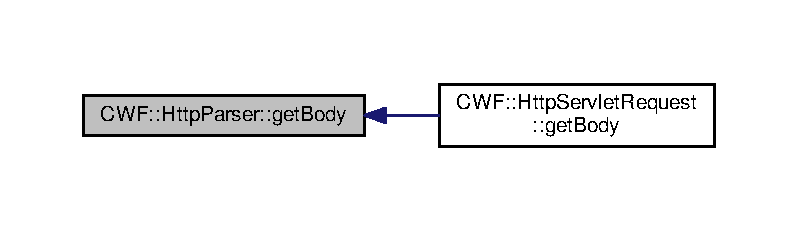
\includegraphics[width=350pt]{class_c_w_f_1_1_http_parser_a4c3be05ffe5ca08abf2e244e08d3de37_icgraph}
\end{center}
\end{figure}


\hypertarget{class_c_w_f_1_1_http_parser_af6b66138a1afe71e15640d4108d426fc}{\index{C\+W\+F\+::\+Http\+Parser@{C\+W\+F\+::\+Http\+Parser}!get\+Content\+Lenght@{get\+Content\+Lenght}}
\index{get\+Content\+Lenght@{get\+Content\+Lenght}!C\+W\+F\+::\+Http\+Parser@{C\+W\+F\+::\+Http\+Parser}}
\subsubsection[{get\+Content\+Lenght}]{\setlength{\rightskip}{0pt plus 5cm}qint64 C\+W\+F\+::\+Http\+Parser\+::get\+Content\+Lenght (
\begin{DoxyParamCaption}
{}
\end{DoxyParamCaption}
) const}}\label{class_c_w_f_1_1_http_parser_af6b66138a1afe71e15640d4108d426fc}
\hypertarget{class_c_w_f_1_1_http_parser_ae25e55945b9b364a20c9f5d3a8696f15}{\index{C\+W\+F\+::\+Http\+Parser@{C\+W\+F\+::\+Http\+Parser}!get\+Content\+Type@{get\+Content\+Type}}
\index{get\+Content\+Type@{get\+Content\+Type}!C\+W\+F\+::\+Http\+Parser@{C\+W\+F\+::\+Http\+Parser}}
\subsubsection[{get\+Content\+Type}]{\setlength{\rightskip}{0pt plus 5cm}Q\+Byte\+Array C\+W\+F\+::\+Http\+Parser\+::get\+Content\+Type (
\begin{DoxyParamCaption}
{}
\end{DoxyParamCaption}
) const}}\label{class_c_w_f_1_1_http_parser_ae25e55945b9b364a20c9f5d3a8696f15}
\hypertarget{class_c_w_f_1_1_http_parser_a0643a4a7672347f8185dd5ffd1016944}{\index{C\+W\+F\+::\+Http\+Parser@{C\+W\+F\+::\+Http\+Parser}!get\+Cookies@{get\+Cookies}}
\index{get\+Cookies@{get\+Cookies}!C\+W\+F\+::\+Http\+Parser@{C\+W\+F\+::\+Http\+Parser}}
\subsubsection[{get\+Cookies}]{\setlength{\rightskip}{0pt plus 5cm}Q\+Vector$<$ {\bf Http\+Cookie} $>$ C\+W\+F\+::\+Http\+Parser\+::get\+Cookies (
\begin{DoxyParamCaption}
{}
\end{DoxyParamCaption}
) const}}\label{class_c_w_f_1_1_http_parser_a0643a4a7672347f8185dd5ffd1016944}
\hypertarget{class_c_w_f_1_1_http_parser_ab171d96734fcd84fedc1ddcc57809130}{\index{C\+W\+F\+::\+Http\+Parser@{C\+W\+F\+::\+Http\+Parser}!get\+Header\+Field@{get\+Header\+Field}}
\index{get\+Header\+Field@{get\+Header\+Field}!C\+W\+F\+::\+Http\+Parser@{C\+W\+F\+::\+Http\+Parser}}
\subsubsection[{get\+Header\+Field}]{\setlength{\rightskip}{0pt plus 5cm}Q\+Byte\+Array C\+W\+F\+::\+Http\+Parser\+::get\+Header\+Field (
\begin{DoxyParamCaption}
\item[{const Q\+Byte\+Array \&}]{header\+Field}
\end{DoxyParamCaption}
) const}}\label{class_c_w_f_1_1_http_parser_ab171d96734fcd84fedc1ddcc57809130}


Here is the caller graph for this function\+:
\nopagebreak
\begin{figure}[H]
\begin{center}
\leavevmode
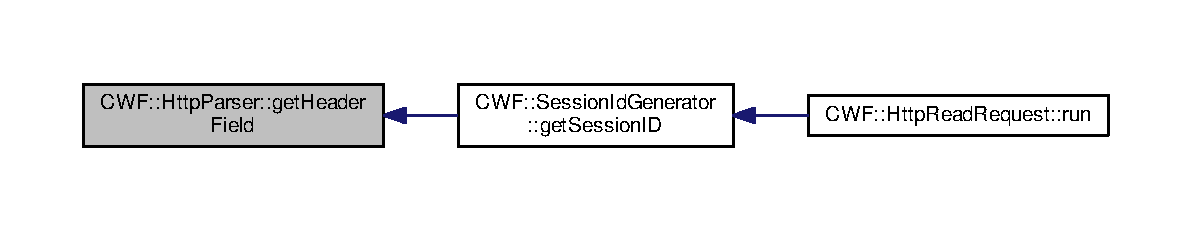
\includegraphics[width=350pt]{class_c_w_f_1_1_http_parser_ab171d96734fcd84fedc1ddcc57809130_icgraph}
\end{center}
\end{figure}


\hypertarget{class_c_w_f_1_1_http_parser_a62ca43a32ee902e94863e3574eb968cb}{\index{C\+W\+F\+::\+Http\+Parser@{C\+W\+F\+::\+Http\+Parser}!get\+Header\+Fields@{get\+Header\+Fields}}
\index{get\+Header\+Fields@{get\+Header\+Fields}!C\+W\+F\+::\+Http\+Parser@{C\+W\+F\+::\+Http\+Parser}}
\subsubsection[{get\+Header\+Fields}]{\setlength{\rightskip}{0pt plus 5cm}Q\+Byte\+Array\+List C\+W\+F\+::\+Http\+Parser\+::get\+Header\+Fields (
\begin{DoxyParamCaption}
\item[{const Q\+Byte\+Array \&}]{header\+Field}
\end{DoxyParamCaption}
) const}}\label{class_c_w_f_1_1_http_parser_a62ca43a32ee902e94863e3574eb968cb}
\hypertarget{class_c_w_f_1_1_http_parser_af8ceae98ad9e63dd30c56409438f4131}{\index{C\+W\+F\+::\+Http\+Parser@{C\+W\+F\+::\+Http\+Parser}!get\+Http\+Version@{get\+Http\+Version}}
\index{get\+Http\+Version@{get\+Http\+Version}!C\+W\+F\+::\+Http\+Parser@{C\+W\+F\+::\+Http\+Parser}}
\subsubsection[{get\+Http\+Version}]{\setlength{\rightskip}{0pt plus 5cm}Q\+Byte\+Array C\+W\+F\+::\+Http\+Parser\+::get\+Http\+Version (
\begin{DoxyParamCaption}
{}
\end{DoxyParamCaption}
) const}}\label{class_c_w_f_1_1_http_parser_af8ceae98ad9e63dd30c56409438f4131}


Here is the caller graph for this function\+:
\nopagebreak
\begin{figure}[H]
\begin{center}
\leavevmode
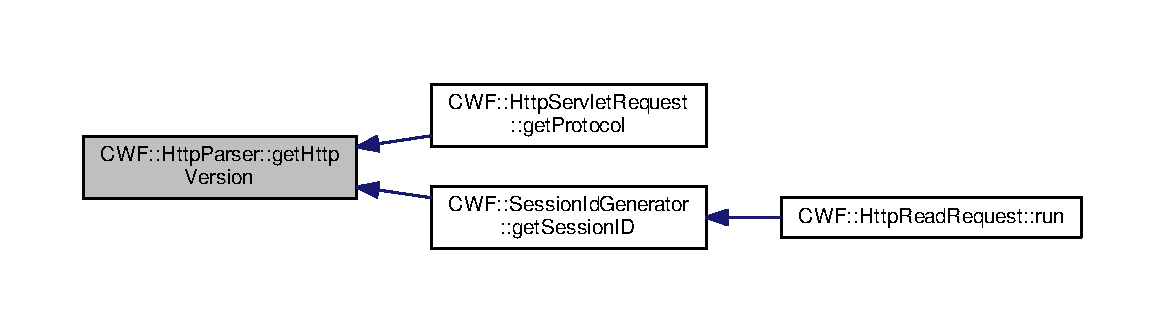
\includegraphics[width=350pt]{class_c_w_f_1_1_http_parser_af8ceae98ad9e63dd30c56409438f4131_icgraph}
\end{center}
\end{figure}


\hypertarget{class_c_w_f_1_1_http_parser_aef9dffb5672f9db22cf2a590dc641706}{\index{C\+W\+F\+::\+Http\+Parser@{C\+W\+F\+::\+Http\+Parser}!get\+Method@{get\+Method}}
\index{get\+Method@{get\+Method}!C\+W\+F\+::\+Http\+Parser@{C\+W\+F\+::\+Http\+Parser}}
\subsubsection[{get\+Method}]{\setlength{\rightskip}{0pt plus 5cm}Q\+Byte\+Array C\+W\+F\+::\+Http\+Parser\+::get\+Method (
\begin{DoxyParamCaption}
{}
\end{DoxyParamCaption}
) const}}\label{class_c_w_f_1_1_http_parser_aef9dffb5672f9db22cf2a590dc641706}


Here is the caller graph for this function\+:
\nopagebreak
\begin{figure}[H]
\begin{center}
\leavevmode
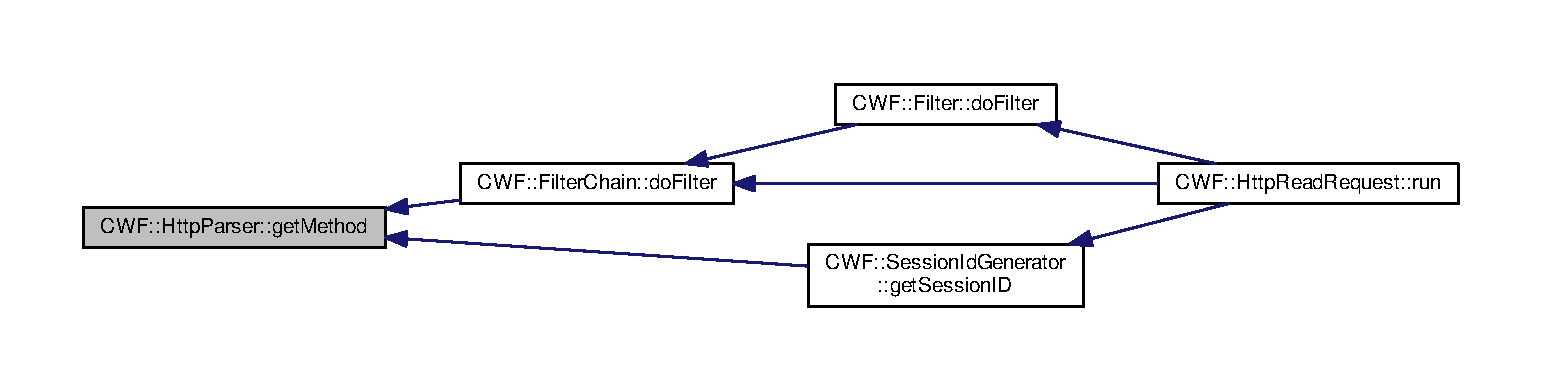
\includegraphics[width=350pt]{class_c_w_f_1_1_http_parser_aef9dffb5672f9db22cf2a590dc641706_icgraph}
\end{center}
\end{figure}


\hypertarget{class_c_w_f_1_1_http_parser_acc4042b879ad71e4c1b82bfb78033a92}{\index{C\+W\+F\+::\+Http\+Parser@{C\+W\+F\+::\+Http\+Parser}!get\+Parameter@{get\+Parameter}}
\index{get\+Parameter@{get\+Parameter}!C\+W\+F\+::\+Http\+Parser@{C\+W\+F\+::\+Http\+Parser}}
\subsubsection[{get\+Parameter}]{\setlength{\rightskip}{0pt plus 5cm}Q\+Byte\+Array C\+W\+F\+::\+Http\+Parser\+::get\+Parameter (
\begin{DoxyParamCaption}
\item[{const Q\+Byte\+Array \&}]{name}
\end{DoxyParamCaption}
) const}}\label{class_c_w_f_1_1_http_parser_acc4042b879ad71e4c1b82bfb78033a92}


Here is the caller graph for this function\+:
\nopagebreak
\begin{figure}[H]
\begin{center}
\leavevmode
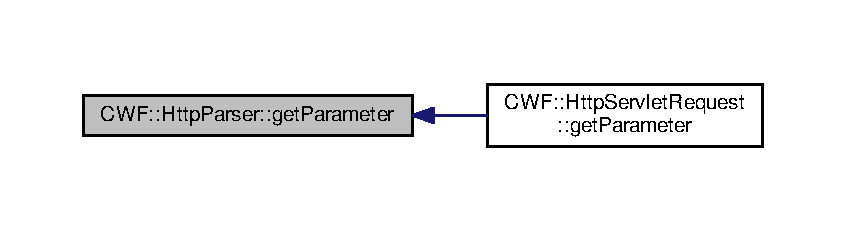
\includegraphics[width=350pt]{class_c_w_f_1_1_http_parser_acc4042b879ad71e4c1b82bfb78033a92_icgraph}
\end{center}
\end{figure}


\hypertarget{class_c_w_f_1_1_http_parser_a0ff9ecad7dd6a5e419e59d7eb0516ee7}{\index{C\+W\+F\+::\+Http\+Parser@{C\+W\+F\+::\+Http\+Parser}!get\+Parameters@{get\+Parameters}}
\index{get\+Parameters@{get\+Parameters}!C\+W\+F\+::\+Http\+Parser@{C\+W\+F\+::\+Http\+Parser}}
\subsubsection[{get\+Parameters}]{\setlength{\rightskip}{0pt plus 5cm}Q\+Byte\+Array\+List C\+W\+F\+::\+Http\+Parser\+::get\+Parameters (
\begin{DoxyParamCaption}
\item[{const Q\+Byte\+Array \&}]{name}
\end{DoxyParamCaption}
) const}}\label{class_c_w_f_1_1_http_parser_a0ff9ecad7dd6a5e419e59d7eb0516ee7}


Here is the caller graph for this function\+:
\nopagebreak
\begin{figure}[H]
\begin{center}
\leavevmode
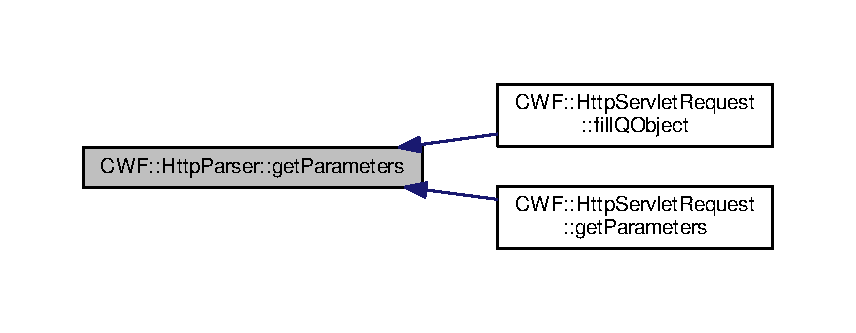
\includegraphics[width=350pt]{class_c_w_f_1_1_http_parser_a0ff9ecad7dd6a5e419e59d7eb0516ee7_icgraph}
\end{center}
\end{figure}


\hypertarget{class_c_w_f_1_1_http_parser_a3991b21e344eac5e60da64a2c1959702}{\index{C\+W\+F\+::\+Http\+Parser@{C\+W\+F\+::\+Http\+Parser}!get\+Parameters@{get\+Parameters}}
\index{get\+Parameters@{get\+Parameters}!C\+W\+F\+::\+Http\+Parser@{C\+W\+F\+::\+Http\+Parser}}
\subsubsection[{get\+Parameters}]{\setlength{\rightskip}{0pt plus 5cm}Q\+Map$<$ Q\+Byte\+Array, Q\+Byte\+Array $>$ C\+W\+F\+::\+Http\+Parser\+::get\+Parameters (
\begin{DoxyParamCaption}
{}
\end{DoxyParamCaption}
) const}}\label{class_c_w_f_1_1_http_parser_a3991b21e344eac5e60da64a2c1959702}
\hypertarget{class_c_w_f_1_1_http_parser_ae448f57d8b83e68f72c208df25fa68c3}{\index{C\+W\+F\+::\+Http\+Parser@{C\+W\+F\+::\+Http\+Parser}!get\+Read\+File@{get\+Read\+File}}
\index{get\+Read\+File@{get\+Read\+File}!C\+W\+F\+::\+Http\+Parser@{C\+W\+F\+::\+Http\+Parser}}
\subsubsection[{get\+Read\+File}]{\setlength{\rightskip}{0pt plus 5cm}bool C\+W\+F\+::\+Http\+Parser\+::get\+Read\+File (
\begin{DoxyParamCaption}
{}
\end{DoxyParamCaption}
) const}}\label{class_c_w_f_1_1_http_parser_ae448f57d8b83e68f72c208df25fa68c3}
\hypertarget{class_c_w_f_1_1_http_parser_a6067d805528a11425f4b58f81218c17f}{\index{C\+W\+F\+::\+Http\+Parser@{C\+W\+F\+::\+Http\+Parser}!get\+Session\+Id@{get\+Session\+Id}}
\index{get\+Session\+Id@{get\+Session\+Id}!C\+W\+F\+::\+Http\+Parser@{C\+W\+F\+::\+Http\+Parser}}
\subsubsection[{get\+Session\+Id}]{\setlength{\rightskip}{0pt plus 5cm}Q\+Byte\+Array C\+W\+F\+::\+Http\+Parser\+::get\+Session\+Id (
\begin{DoxyParamCaption}
{}
\end{DoxyParamCaption}
) const}}\label{class_c_w_f_1_1_http_parser_a6067d805528a11425f4b58f81218c17f}
\hypertarget{class_c_w_f_1_1_http_parser_a1f1f898cb71d02928d733d04e882a2eb}{\index{C\+W\+F\+::\+Http\+Parser@{C\+W\+F\+::\+Http\+Parser}!get\+Uploaded\+Files@{get\+Uploaded\+Files}}
\index{get\+Uploaded\+Files@{get\+Uploaded\+Files}!C\+W\+F\+::\+Http\+Parser@{C\+W\+F\+::\+Http\+Parser}}
\subsubsection[{get\+Uploaded\+Files}]{\setlength{\rightskip}{0pt plus 5cm}Q\+Multi\+Map$<$ Q\+Byte\+Array, Q\+Byte\+Array $>$ C\+W\+F\+::\+Http\+Parser\+::get\+Uploaded\+Files (
\begin{DoxyParamCaption}
{}
\end{DoxyParamCaption}
) const}}\label{class_c_w_f_1_1_http_parser_a1f1f898cb71d02928d733d04e882a2eb}


Here is the caller graph for this function\+:
\nopagebreak
\begin{figure}[H]
\begin{center}
\leavevmode
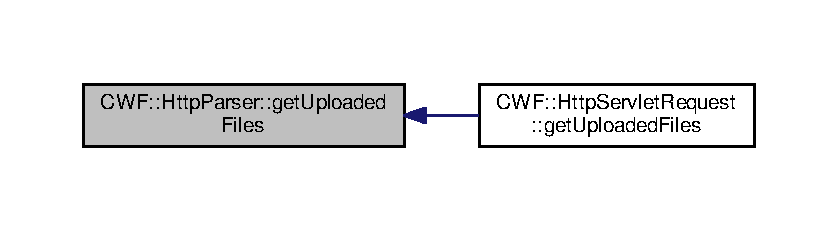
\includegraphics[width=350pt]{class_c_w_f_1_1_http_parser_a1f1f898cb71d02928d733d04e882a2eb_icgraph}
\end{center}
\end{figure}


\hypertarget{class_c_w_f_1_1_http_parser_ab6e2249f05ad5a7a25ace2e36066e57b}{\index{C\+W\+F\+::\+Http\+Parser@{C\+W\+F\+::\+Http\+Parser}!get\+Url@{get\+Url}}
\index{get\+Url@{get\+Url}!C\+W\+F\+::\+Http\+Parser@{C\+W\+F\+::\+Http\+Parser}}
\subsubsection[{get\+Url}]{\setlength{\rightskip}{0pt plus 5cm}Q\+Byte\+Array C\+W\+F\+::\+Http\+Parser\+::get\+Url (
\begin{DoxyParamCaption}
{}
\end{DoxyParamCaption}
) const}}\label{class_c_w_f_1_1_http_parser_ab6e2249f05ad5a7a25ace2e36066e57b}


Here is the caller graph for this function\+:
\nopagebreak
\begin{figure}[H]
\begin{center}
\leavevmode
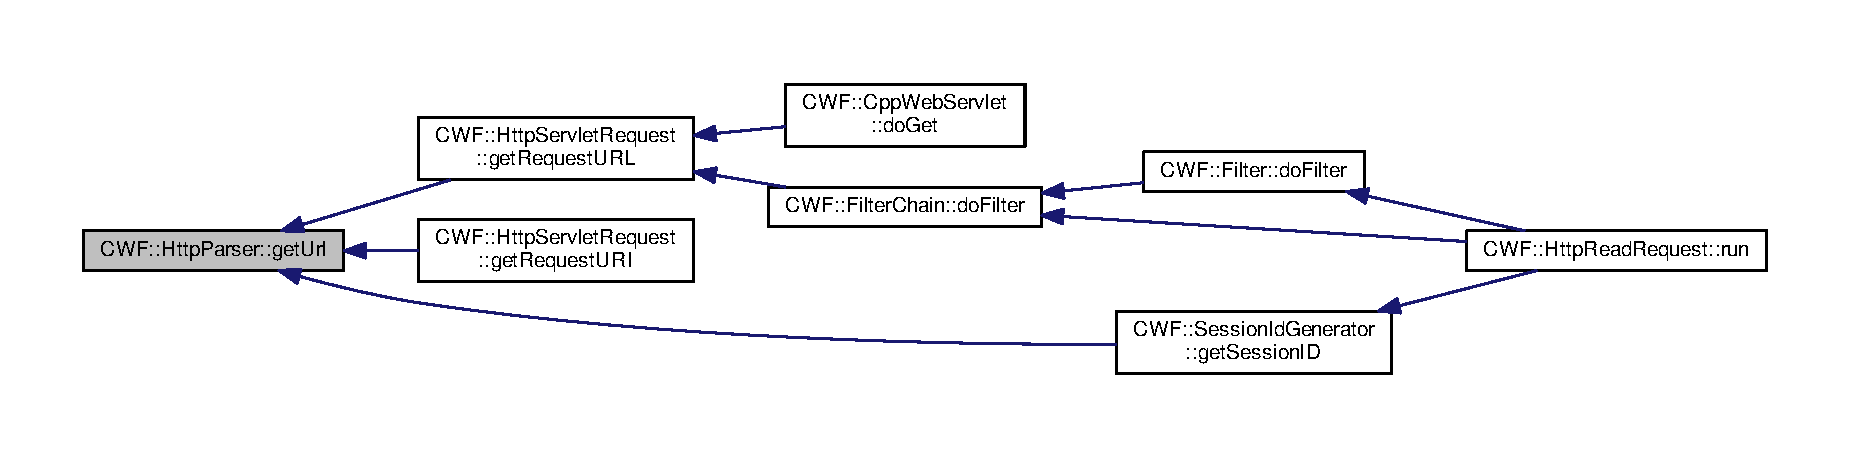
\includegraphics[width=350pt]{class_c_w_f_1_1_http_parser_ab6e2249f05ad5a7a25ace2e36066e57b_icgraph}
\end{center}
\end{figure}


\hypertarget{class_c_w_f_1_1_http_parser_a25a2d703b1ad5d2e660b63decf05800f}{\index{C\+W\+F\+::\+Http\+Parser@{C\+W\+F\+::\+Http\+Parser}!is\+Multi\+Part@{is\+Multi\+Part}}
\index{is\+Multi\+Part@{is\+Multi\+Part}!C\+W\+F\+::\+Http\+Parser@{C\+W\+F\+::\+Http\+Parser}}
\subsubsection[{is\+Multi\+Part}]{\setlength{\rightskip}{0pt plus 5cm}bool C\+W\+F\+::\+Http\+Parser\+::is\+Multi\+Part (
\begin{DoxyParamCaption}
{}
\end{DoxyParamCaption}
) const}}\label{class_c_w_f_1_1_http_parser_a25a2d703b1ad5d2e660b63decf05800f}
\hypertarget{class_c_w_f_1_1_http_parser_a389b222c042abe6ce98412d43b6af4c2}{\index{C\+W\+F\+::\+Http\+Parser@{C\+W\+F\+::\+Http\+Parser}!is\+Valid@{is\+Valid}}
\index{is\+Valid@{is\+Valid}!C\+W\+F\+::\+Http\+Parser@{C\+W\+F\+::\+Http\+Parser}}
\subsubsection[{is\+Valid}]{\setlength{\rightskip}{0pt plus 5cm}bool C\+W\+F\+::\+Http\+Parser\+::is\+Valid (
\begin{DoxyParamCaption}
{}
\end{DoxyParamCaption}
) const}}\label{class_c_w_f_1_1_http_parser_a389b222c042abe6ce98412d43b6af4c2}


\subsection{Friends And Related Function Documentation}
\hypertarget{class_c_w_f_1_1_http_parser_a4d54f5003e07e218070a449c22a52c7c}{\index{C\+W\+F\+::\+Http\+Parser@{C\+W\+F\+::\+Http\+Parser}!Http\+Read\+Request@{Http\+Read\+Request}}
\index{Http\+Read\+Request@{Http\+Read\+Request}!C\+W\+F\+::\+Http\+Parser@{C\+W\+F\+::\+Http\+Parser}}
\subsubsection[{Http\+Read\+Request}]{\setlength{\rightskip}{0pt plus 5cm}friend class {\bf Http\+Read\+Request}\hspace{0.3cm}{\ttfamily [friend]}}}\label{class_c_w_f_1_1_http_parser_a4d54f5003e07e218070a449c22a52c7c}


The documentation for this class was generated from the following files\+:\begin{DoxyCompactItemize}
\item 
/home/herik/\+C\+P\+P\+Web\+Framework/\+C\+P\+P\+Web\+Framework/cwf/\hyperlink{httpparser_8h}{httpparser.\+h}\item 
/home/herik/\+C\+P\+P\+Web\+Framework/\+C\+P\+P\+Web\+Framework/cwf/\hyperlink{httpparser_8cpp}{httpparser.\+cpp}\end{DoxyCompactItemize}

\hypertarget{class_c_w_f_1_1_http_read_request}{\section{C\+W\+F\+:\+:Http\+Read\+Request Class Reference}
\label{class_c_w_f_1_1_http_read_request}\index{C\+W\+F\+::\+Http\+Read\+Request@{C\+W\+F\+::\+Http\+Read\+Request}}
}


The \hyperlink{class_c_w_f_1_1_http_read_request}{Http\+Read\+Request} class is created automatically by the \hyperlink{class_c_w_f_1_1_cpp_web_server}{Cpp\+Web\+Server} and inserted ~\newline
 in a Q\+Thread\+Pool, always when the \hyperlink{class_c_w_f_1_1_cpp_web_server}{Cpp\+Web\+Server} has a call by a client(\+Browser).  




{\ttfamily \#include $<$httpreadrequest.\+h$>$}



Inheritance diagram for C\+W\+F\+:\+:Http\+Read\+Request\+:
\nopagebreak
\begin{figure}[H]
\begin{center}
\leavevmode
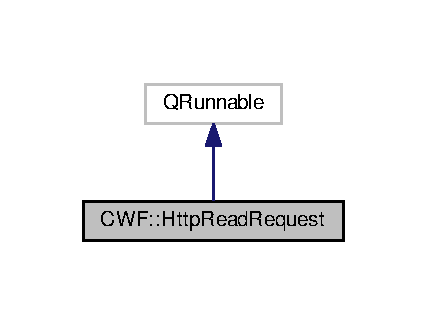
\includegraphics[width=205pt]{class_c_w_f_1_1_http_read_request__inherit__graph}
\end{center}
\end{figure}
\subsection*{Public Member Functions}
\begin{DoxyCompactItemize}
\item 
\hyperlink{class_c_w_f_1_1_http_read_request_ade7aa5ac198bb40ce98de9f9ac9ff4d2}{Http\+Read\+Request} (qintptr socket\+Descriptor, \hyperlink{class_c_w_f_1_1_q_map_thread_safety}{Q\+Map\+Thread\+Safety}$<$ Q\+String, \hyperlink{class_c_w_f_1_1_http_servlet}{Http\+Servlet} $\ast$ $>$ \&url\+Servlet, \hyperlink{class_c_w_f_1_1_q_map_thread_safety}{Q\+Map\+Thread\+Safety}$<$ Q\+String, \hyperlink{class_c_w_f_1_1_http_session}{Http\+Session} $\ast$ $>$ \&sessions, Q\+Ssl\+Configuration $\ast$ssl\+Configuration, \hyperlink{class_c_w_f_1_1_filter}{Filter} $\ast$filter)
\begin{DoxyCompactList}\small\item\em This constructor needs to receive the parent, a socket descriptor, all the mapped servlets, all the sessions,~\newline
 a filter, the default path to the pages and resources like\+: xhtml pages, images, css...~\newline
 a domain, and a session expire time to the sessions(optional). \end{DoxyCompactList}\item 
\hyperlink{class_c_w_f_1_1_http_read_request_ad2013577721f188ab3e94c9b977fe3ee}{$\sim$\+Http\+Read\+Request} ()
\begin{DoxyCompactList}\small\item\em Starts to read the requisition. \end{DoxyCompactList}\item 
void \hyperlink{class_c_w_f_1_1_http_read_request_a45c1183b9857a34d4a53452917f7bcec}{run} ()
\end{DoxyCompactItemize}


\subsection{Detailed Description}
The \hyperlink{class_c_w_f_1_1_http_read_request}{Http\+Read\+Request} class is created automatically by the \hyperlink{class_c_w_f_1_1_cpp_web_server}{Cpp\+Web\+Server} and inserted ~\newline
 in a Q\+Thread\+Pool, always when the \hyperlink{class_c_w_f_1_1_cpp_web_server}{Cpp\+Web\+Server} has a call by a client(\+Browser). 

\subsection{Constructor \& Destructor Documentation}
\hypertarget{class_c_w_f_1_1_http_read_request_ade7aa5ac198bb40ce98de9f9ac9ff4d2}{\index{C\+W\+F\+::\+Http\+Read\+Request@{C\+W\+F\+::\+Http\+Read\+Request}!Http\+Read\+Request@{Http\+Read\+Request}}
\index{Http\+Read\+Request@{Http\+Read\+Request}!C\+W\+F\+::\+Http\+Read\+Request@{C\+W\+F\+::\+Http\+Read\+Request}}
\subsubsection[{Http\+Read\+Request}]{\setlength{\rightskip}{0pt plus 5cm}C\+W\+F\+::\+Http\+Read\+Request\+::\+Http\+Read\+Request (
\begin{DoxyParamCaption}
\item[{qintptr}]{socket\+Descriptor, }
\item[{{\bf Q\+Map\+Thread\+Safety}$<$ Q\+String, {\bf Http\+Servlet} $\ast$ $>$ \&}]{url\+Servlet, }
\item[{{\bf Q\+Map\+Thread\+Safety}$<$ Q\+String, {\bf Http\+Session} $\ast$ $>$ \&}]{sessions, }
\item[{Q\+Ssl\+Configuration $\ast$}]{ssl\+Configuration, }
\item[{{\bf Filter} $\ast$}]{filter}
\end{DoxyParamCaption}
)}}\label{class_c_w_f_1_1_http_read_request_ade7aa5ac198bb40ce98de9f9ac9ff4d2}


This constructor needs to receive the parent, a socket descriptor, all the mapped servlets, all the sessions,~\newline
 a filter, the default path to the pages and resources like\+: xhtml pages, images, css...~\newline
 a domain, and a session expire time to the sessions(optional). 


\begin{DoxyParams}{Parameters}
{\em parent} & \+: This is a pointer to Q\+Object. \\
\hline
{\em socket\+Descriptor} & \+: This is a qintptr. \\
\hline
{\em url\+Servlet} & \+: This is a reference to a \hyperlink{class_c_w_f_1_1_q_map_thread_safety}{Q\+Map\+Thread\+Safety}. \\
\hline
{\em sessions} & \+: This is a reference to a \hyperlink{class_c_w_f_1_1_q_map_thread_safety}{Q\+Map\+Thread\+Safety}. \\
\hline
{\em filter} & \+: This is a pointer to a \hyperlink{class_c_w_f_1_1_filter}{Filter}. \\
\hline
{\em path} & \+: This is a reference to a Q\+String. \\
\hline
{\em domain} & \+: This is a reference to a Q\+String. \\
\hline
{\em session\+Expiration\+Time} & \+: This is a qint64. \\
\hline
\end{DoxyParams}
\hypertarget{class_c_w_f_1_1_http_read_request_ad2013577721f188ab3e94c9b977fe3ee}{\index{C\+W\+F\+::\+Http\+Read\+Request@{C\+W\+F\+::\+Http\+Read\+Request}!````~Http\+Read\+Request@{$\sim$\+Http\+Read\+Request}}
\index{````~Http\+Read\+Request@{$\sim$\+Http\+Read\+Request}!C\+W\+F\+::\+Http\+Read\+Request@{C\+W\+F\+::\+Http\+Read\+Request}}
\subsubsection[{$\sim$\+Http\+Read\+Request}]{\setlength{\rightskip}{0pt plus 5cm}C\+W\+F\+::\+Http\+Read\+Request\+::$\sim$\+Http\+Read\+Request (
\begin{DoxyParamCaption}
{}
\end{DoxyParamCaption}
)}}\label{class_c_w_f_1_1_http_read_request_ad2013577721f188ab3e94c9b977fe3ee}


Starts to read the requisition. 



\subsection{Member Function Documentation}
\hypertarget{class_c_w_f_1_1_http_read_request_a45c1183b9857a34d4a53452917f7bcec}{\index{C\+W\+F\+::\+Http\+Read\+Request@{C\+W\+F\+::\+Http\+Read\+Request}!run@{run}}
\index{run@{run}!C\+W\+F\+::\+Http\+Read\+Request@{C\+W\+F\+::\+Http\+Read\+Request}}
\subsubsection[{run}]{\setlength{\rightskip}{0pt plus 5cm}void C\+W\+F\+::\+Http\+Read\+Request\+::run (
\begin{DoxyParamCaption}
{}
\end{DoxyParamCaption}
)}}\label{class_c_w_f_1_1_http_read_request_a45c1183b9857a34d4a53452917f7bcec}


The documentation for this class was generated from the following files\+:\begin{DoxyCompactItemize}
\item 
/home/herik/\+C\+P\+P\+Web\+Framework/\+C\+P\+P\+Web\+Framework/cwf/\hyperlink{httpreadrequest_8h}{httpreadrequest.\+h}\item 
/home/herik/\+C\+P\+P\+Web\+Framework/\+C\+P\+P\+Web\+Framework/cwf/\hyperlink{httpreadrequest_8cpp}{httpreadrequest.\+cpp}\end{DoxyCompactItemize}

\hypertarget{class_c_w_f_1_1_http_request_method}{\section{C\+W\+F\+:\+:Http\+Request\+Method Class Reference}
\label{class_c_w_f_1_1_http_request_method}\index{C\+W\+F\+::\+Http\+Request\+Method@{C\+W\+F\+::\+Http\+Request\+Method}}
}


The \hyperlink{class_c_w_f_1_1_http_request_method}{Http\+Request\+Method} class holds fixed strings that represents request methods.  




{\ttfamily \#include $<$httprequestmethod.\+h$>$}

\subsection*{Static Public Member Functions}
\begin{DoxyCompactItemize}
\item 
static const Q\+String \hyperlink{class_c_w_f_1_1_http_request_method_ad63561f9453c2362e1758ceb964accd6}{get\+Delete} ()
\begin{DoxyCompactList}\small\item\em This is a static method and returns a string to the delete request method. \end{DoxyCompactList}\item 
static const Q\+String \hyperlink{class_c_w_f_1_1_http_request_method_ad6e58fa2e06927cb4ce3ff19c3f4369f}{get\+Get} ()
\begin{DoxyCompactList}\small\item\em This is a static method and returns a string to the get request method. \end{DoxyCompactList}\item 
static const Q\+String \hyperlink{class_c_w_f_1_1_http_request_method_adc2dd58856fc6aca290e039589f2c6d7}{get\+Head} ()
\begin{DoxyCompactList}\small\item\em This is a static method and returns a string to the head request method. \end{DoxyCompactList}\item 
static const Q\+String \hyperlink{class_c_w_f_1_1_http_request_method_a682a34e04ff2fcc5ff71d1e35ea296e2}{get\+Options} ()
\begin{DoxyCompactList}\small\item\em This is a static method and returns a string to the options request method. \end{DoxyCompactList}\item 
static const Q\+String \hyperlink{class_c_w_f_1_1_http_request_method_a29593550f01b15a1b67c627e75b9a14a}{get\+Post} ()
\begin{DoxyCompactList}\small\item\em This is a static method and returns a string to the post request method. \end{DoxyCompactList}\item 
static const Q\+String \hyperlink{class_c_w_f_1_1_http_request_method_a11a56340e3b597802c7166a1083a4ea6}{get\+Put} ()
\begin{DoxyCompactList}\small\item\em This is a static method and returns a string to the put request method. \end{DoxyCompactList}\item 
static const Q\+String \hyperlink{class_c_w_f_1_1_http_request_method_a581cae139792fb05da6cb5fcbdc7d8f7}{get\+Trace} ()
\begin{DoxyCompactList}\small\item\em This is a static method and returns a string to the trace request method. \end{DoxyCompactList}\end{DoxyCompactItemize}


\subsection{Detailed Description}
The \hyperlink{class_c_w_f_1_1_http_request_method}{Http\+Request\+Method} class holds fixed strings that represents request methods. 

\subsection{Member Function Documentation}
\hypertarget{class_c_w_f_1_1_http_request_method_ad63561f9453c2362e1758ceb964accd6}{\index{C\+W\+F\+::\+Http\+Request\+Method@{C\+W\+F\+::\+Http\+Request\+Method}!get\+Delete@{get\+Delete}}
\index{get\+Delete@{get\+Delete}!C\+W\+F\+::\+Http\+Request\+Method@{C\+W\+F\+::\+Http\+Request\+Method}}
\subsubsection[{get\+Delete}]{\setlength{\rightskip}{0pt plus 5cm}static const Q\+String C\+W\+F\+::\+Http\+Request\+Method\+::get\+Delete (
\begin{DoxyParamCaption}
{}
\end{DoxyParamCaption}
)\hspace{0.3cm}{\ttfamily [inline]}, {\ttfamily [static]}}}\label{class_c_w_f_1_1_http_request_method_ad63561f9453c2362e1758ceb964accd6}


This is a static method and returns a string to the delete request method. 

\begin{DoxyReturn}{Returns}
Q\+String \+: Returns \char`\"{}\+D\+E\+L\+E\+T\+E\char`\"{} 
\end{DoxyReturn}
\hypertarget{class_c_w_f_1_1_http_request_method_ad6e58fa2e06927cb4ce3ff19c3f4369f}{\index{C\+W\+F\+::\+Http\+Request\+Method@{C\+W\+F\+::\+Http\+Request\+Method}!get\+Get@{get\+Get}}
\index{get\+Get@{get\+Get}!C\+W\+F\+::\+Http\+Request\+Method@{C\+W\+F\+::\+Http\+Request\+Method}}
\subsubsection[{get\+Get}]{\setlength{\rightskip}{0pt plus 5cm}static const Q\+String C\+W\+F\+::\+Http\+Request\+Method\+::get\+Get (
\begin{DoxyParamCaption}
{}
\end{DoxyParamCaption}
)\hspace{0.3cm}{\ttfamily [inline]}, {\ttfamily [static]}}}\label{class_c_w_f_1_1_http_request_method_ad6e58fa2e06927cb4ce3ff19c3f4369f}


This is a static method and returns a string to the get request method. 

\begin{DoxyReturn}{Returns}
Q\+String \+: Returns \char`\"{}\+G\+E\+T\char`\"{} 
\end{DoxyReturn}
\hypertarget{class_c_w_f_1_1_http_request_method_adc2dd58856fc6aca290e039589f2c6d7}{\index{C\+W\+F\+::\+Http\+Request\+Method@{C\+W\+F\+::\+Http\+Request\+Method}!get\+Head@{get\+Head}}
\index{get\+Head@{get\+Head}!C\+W\+F\+::\+Http\+Request\+Method@{C\+W\+F\+::\+Http\+Request\+Method}}
\subsubsection[{get\+Head}]{\setlength{\rightskip}{0pt plus 5cm}static const Q\+String C\+W\+F\+::\+Http\+Request\+Method\+::get\+Head (
\begin{DoxyParamCaption}
{}
\end{DoxyParamCaption}
)\hspace{0.3cm}{\ttfamily [inline]}, {\ttfamily [static]}}}\label{class_c_w_f_1_1_http_request_method_adc2dd58856fc6aca290e039589f2c6d7}


This is a static method and returns a string to the head request method. 

\begin{DoxyReturn}{Returns}
Q\+String \+: Returns \char`\"{}\+H\+E\+A\+D\char`\"{} 
\end{DoxyReturn}
\hypertarget{class_c_w_f_1_1_http_request_method_a682a34e04ff2fcc5ff71d1e35ea296e2}{\index{C\+W\+F\+::\+Http\+Request\+Method@{C\+W\+F\+::\+Http\+Request\+Method}!get\+Options@{get\+Options}}
\index{get\+Options@{get\+Options}!C\+W\+F\+::\+Http\+Request\+Method@{C\+W\+F\+::\+Http\+Request\+Method}}
\subsubsection[{get\+Options}]{\setlength{\rightskip}{0pt plus 5cm}static const Q\+String C\+W\+F\+::\+Http\+Request\+Method\+::get\+Options (
\begin{DoxyParamCaption}
{}
\end{DoxyParamCaption}
)\hspace{0.3cm}{\ttfamily [inline]}, {\ttfamily [static]}}}\label{class_c_w_f_1_1_http_request_method_a682a34e04ff2fcc5ff71d1e35ea296e2}


This is a static method and returns a string to the options request method. 

\begin{DoxyReturn}{Returns}
Q\+String \+: Returns \char`\"{}\+O\+P\+T\+I\+O\+N\+S\char`\"{} 
\end{DoxyReturn}
\hypertarget{class_c_w_f_1_1_http_request_method_a29593550f01b15a1b67c627e75b9a14a}{\index{C\+W\+F\+::\+Http\+Request\+Method@{C\+W\+F\+::\+Http\+Request\+Method}!get\+Post@{get\+Post}}
\index{get\+Post@{get\+Post}!C\+W\+F\+::\+Http\+Request\+Method@{C\+W\+F\+::\+Http\+Request\+Method}}
\subsubsection[{get\+Post}]{\setlength{\rightskip}{0pt plus 5cm}static const Q\+String C\+W\+F\+::\+Http\+Request\+Method\+::get\+Post (
\begin{DoxyParamCaption}
{}
\end{DoxyParamCaption}
)\hspace{0.3cm}{\ttfamily [inline]}, {\ttfamily [static]}}}\label{class_c_w_f_1_1_http_request_method_a29593550f01b15a1b67c627e75b9a14a}


This is a static method and returns a string to the post request method. 

\begin{DoxyReturn}{Returns}
Q\+String \+: Returns \char`\"{}\+P\+O\+S\+T\char`\"{} 
\end{DoxyReturn}
\hypertarget{class_c_w_f_1_1_http_request_method_a11a56340e3b597802c7166a1083a4ea6}{\index{C\+W\+F\+::\+Http\+Request\+Method@{C\+W\+F\+::\+Http\+Request\+Method}!get\+Put@{get\+Put}}
\index{get\+Put@{get\+Put}!C\+W\+F\+::\+Http\+Request\+Method@{C\+W\+F\+::\+Http\+Request\+Method}}
\subsubsection[{get\+Put}]{\setlength{\rightskip}{0pt plus 5cm}static const Q\+String C\+W\+F\+::\+Http\+Request\+Method\+::get\+Put (
\begin{DoxyParamCaption}
{}
\end{DoxyParamCaption}
)\hspace{0.3cm}{\ttfamily [inline]}, {\ttfamily [static]}}}\label{class_c_w_f_1_1_http_request_method_a11a56340e3b597802c7166a1083a4ea6}


This is a static method and returns a string to the put request method. 

\begin{DoxyReturn}{Returns}
Q\+String \+: Returns \char`\"{}\+P\+U\+T\char`\"{} 
\end{DoxyReturn}
\hypertarget{class_c_w_f_1_1_http_request_method_a581cae139792fb05da6cb5fcbdc7d8f7}{\index{C\+W\+F\+::\+Http\+Request\+Method@{C\+W\+F\+::\+Http\+Request\+Method}!get\+Trace@{get\+Trace}}
\index{get\+Trace@{get\+Trace}!C\+W\+F\+::\+Http\+Request\+Method@{C\+W\+F\+::\+Http\+Request\+Method}}
\subsubsection[{get\+Trace}]{\setlength{\rightskip}{0pt plus 5cm}static const Q\+String C\+W\+F\+::\+Http\+Request\+Method\+::get\+Trace (
\begin{DoxyParamCaption}
{}
\end{DoxyParamCaption}
)\hspace{0.3cm}{\ttfamily [inline]}, {\ttfamily [static]}}}\label{class_c_w_f_1_1_http_request_method_a581cae139792fb05da6cb5fcbdc7d8f7}


This is a static method and returns a string to the trace request method. 

\begin{DoxyReturn}{Returns}
Q\+String \+: Returns \char`\"{}\+T\+R\+A\+C\+E\char`\"{} 
\end{DoxyReturn}


The documentation for this class was generated from the following file\+:\begin{DoxyCompactItemize}
\item 
/home/herik/\+C\+P\+P\+Web\+Framework/\+C\+P\+P\+Web\+Framework/cwf/\hyperlink{httprequestmethod_8h}{httprequestmethod.\+h}\end{DoxyCompactItemize}

\hypertarget{class_c_w_f_1_1_http_servlet}{\section{C\+W\+F\+:\+:Http\+Servlet Class Reference}
\label{class_c_w_f_1_1_http_servlet}\index{C\+W\+F\+::\+Http\+Servlet@{C\+W\+F\+::\+Http\+Servlet}}
}


The \hyperlink{class_c_w_f_1_1_http_servlet}{Http\+Servlet} class is responsable to attend a request from a specific url. You will need to create a derived class from \hyperlink{class_c_w_f_1_1_http_servlet}{Http\+Servlet} and then, reconstruct the desired method to response a request, after this, you will need mapping the url to the new servlet that you created, you need to do it into the Configure\+Cpp\+Web\+Server using the method add\+Url\+Servlet.  




{\ttfamily \#include $<$httpservlet.\+h$>$}



Inheritance diagram for C\+W\+F\+:\+:Http\+Servlet\+:\nopagebreak
\begin{figure}[H]
\begin{center}
\leavevmode
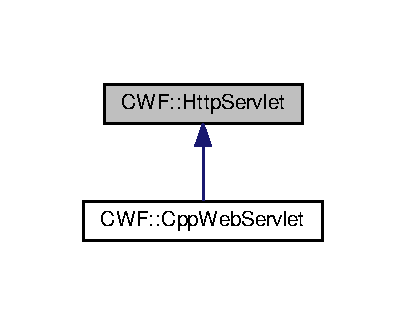
\includegraphics[width=195pt]{class_c_w_f_1_1_http_servlet__inherit__graph}
\end{center}
\end{figure}
\subsection*{Public Member Functions}
\begin{DoxyCompactItemize}
\item 
virtual \hyperlink{class_c_w_f_1_1_http_servlet_a62a6b834356c237ad9787d838d0b8776}{$\sim$\+Http\+Servlet} ()
\begin{DoxyCompactList}\small\item\em Destructor. \end{DoxyCompactList}\item 
virtual void \hyperlink{class_c_w_f_1_1_http_servlet_a10f9bd01fac297a92c39e4eb3ca652fe}{do\+Delete} (\hyperlink{class_c_w_f_1_1_http_servlet_request}{Http\+Servlet\+Request} \&req, \hyperlink{class_c_w_f_1_1_http_servlet_response}{Http\+Servlet\+Response} \&resp)
\begin{DoxyCompactList}\small\item\em This is an virtual method that can be overloaded to attend the delete request method. \end{DoxyCompactList}\item 
virtual void \hyperlink{class_c_w_f_1_1_http_servlet_ad05501d3611f28b20d2c045515119f20}{do\+Get} (\hyperlink{class_c_w_f_1_1_http_servlet_request}{Http\+Servlet\+Request} \&req, \hyperlink{class_c_w_f_1_1_http_servlet_response}{Http\+Servlet\+Response} \&resp)
\begin{DoxyCompactList}\small\item\em This is an virtual method that can be overloaded to attend the get request method. \end{DoxyCompactList}\item 
virtual void \hyperlink{class_c_w_f_1_1_http_servlet_afa172deaf51e527c474ccdd093075e91}{do\+Options} (\hyperlink{class_c_w_f_1_1_http_servlet_request}{Http\+Servlet\+Request} \&req, \hyperlink{class_c_w_f_1_1_http_servlet_response}{Http\+Servlet\+Response} \&resp)
\begin{DoxyCompactList}\small\item\em This is an virtual method that can be overloaded to attend the options request method. \end{DoxyCompactList}\item 
virtual void \hyperlink{class_c_w_f_1_1_http_servlet_a65ddc8bb71865d748c1b1b3303e593b3}{do\+Post} (\hyperlink{class_c_w_f_1_1_http_servlet_request}{Http\+Servlet\+Request} \&req, \hyperlink{class_c_w_f_1_1_http_servlet_response}{Http\+Servlet\+Response} \&resp)
\begin{DoxyCompactList}\small\item\em This is an virtual method that can be overloaded to attend the post request method. \end{DoxyCompactList}\item 
virtual void \hyperlink{class_c_w_f_1_1_http_servlet_a847d042eaebf7fbe02a0ab718bdded0f}{do\+Put} (\hyperlink{class_c_w_f_1_1_http_servlet_request}{Http\+Servlet\+Request} \&req, \hyperlink{class_c_w_f_1_1_http_servlet_response}{Http\+Servlet\+Response} \&resp)
\begin{DoxyCompactList}\small\item\em This is an virtual method that can be overloaded to attend the put request method. \end{DoxyCompactList}\item 
virtual void \hyperlink{class_c_w_f_1_1_http_servlet_aaa4d7914915bdbf290245365dba85367}{do\+Trace} (\hyperlink{class_c_w_f_1_1_http_servlet_request}{Http\+Servlet\+Request} \&req, \hyperlink{class_c_w_f_1_1_http_servlet_response}{Http\+Servlet\+Response} \&resp)
\begin{DoxyCompactList}\small\item\em This is an virtual method that can be overloaded to attend the trace request method. \end{DoxyCompactList}\end{DoxyCompactItemize}


\subsection{Detailed Description}
The \hyperlink{class_c_w_f_1_1_http_servlet}{Http\+Servlet} class is responsable to attend a request from a specific url. You will need to create a derived class from \hyperlink{class_c_w_f_1_1_http_servlet}{Http\+Servlet} and then, reconstruct the desired method to response a request, after this, you will need mapping the url to the new servlet that you created, you need to do it into the Configure\+Cpp\+Web\+Server using the method add\+Url\+Servlet. 

\subsection{Constructor \& Destructor Documentation}
\hypertarget{class_c_w_f_1_1_http_servlet_a62a6b834356c237ad9787d838d0b8776}{\index{C\+W\+F\+::\+Http\+Servlet@{C\+W\+F\+::\+Http\+Servlet}!````~Http\+Servlet@{$\sim$\+Http\+Servlet}}
\index{````~Http\+Servlet@{$\sim$\+Http\+Servlet}!C\+W\+F\+::\+Http\+Servlet@{C\+W\+F\+::\+Http\+Servlet}}
\subsubsection[{$\sim$\+Http\+Servlet}]{\setlength{\rightskip}{0pt plus 5cm}C\+W\+F\+::\+Http\+Servlet\+::$\sim$\+Http\+Servlet (
\begin{DoxyParamCaption}
{}
\end{DoxyParamCaption}
)\hspace{0.3cm}{\ttfamily [virtual]}}}\label{class_c_w_f_1_1_http_servlet_a62a6b834356c237ad9787d838d0b8776}


Destructor. 



\subsection{Member Function Documentation}
\hypertarget{class_c_w_f_1_1_http_servlet_a10f9bd01fac297a92c39e4eb3ca652fe}{\index{C\+W\+F\+::\+Http\+Servlet@{C\+W\+F\+::\+Http\+Servlet}!do\+Delete@{do\+Delete}}
\index{do\+Delete@{do\+Delete}!C\+W\+F\+::\+Http\+Servlet@{C\+W\+F\+::\+Http\+Servlet}}
\subsubsection[{do\+Delete}]{\setlength{\rightskip}{0pt plus 5cm}void C\+W\+F\+::\+Http\+Servlet\+::do\+Delete (
\begin{DoxyParamCaption}
\item[{{\bf Http\+Servlet\+Request} \&}]{req, }
\item[{{\bf Http\+Servlet\+Response} \&}]{resp}
\end{DoxyParamCaption}
)\hspace{0.3cm}{\ttfamily [virtual]}}}\label{class_c_w_f_1_1_http_servlet_a10f9bd01fac297a92c39e4eb3ca652fe}


This is an virtual method that can be overloaded to attend the delete request method. 


\begin{DoxyParams}{Parameters}
{\em req} & \+: This is a reference to the \hyperlink{class_c_w_f_1_1_http_servlet_request}{Http\+Servlet\+Request}. \\
\hline
{\em resp} & \+: This is a reference to the \hyperlink{class_c_w_f_1_1_http_servlet_response}{Http\+Servlet\+Response}. \\
\hline
\end{DoxyParams}
\hypertarget{class_c_w_f_1_1_http_servlet_ad05501d3611f28b20d2c045515119f20}{\index{C\+W\+F\+::\+Http\+Servlet@{C\+W\+F\+::\+Http\+Servlet}!do\+Get@{do\+Get}}
\index{do\+Get@{do\+Get}!C\+W\+F\+::\+Http\+Servlet@{C\+W\+F\+::\+Http\+Servlet}}
\subsubsection[{do\+Get}]{\setlength{\rightskip}{0pt plus 5cm}void C\+W\+F\+::\+Http\+Servlet\+::do\+Get (
\begin{DoxyParamCaption}
\item[{{\bf Http\+Servlet\+Request} \&}]{req, }
\item[{{\bf Http\+Servlet\+Response} \&}]{resp}
\end{DoxyParamCaption}
)\hspace{0.3cm}{\ttfamily [virtual]}}}\label{class_c_w_f_1_1_http_servlet_ad05501d3611f28b20d2c045515119f20}


This is an virtual method that can be overloaded to attend the get request method. 


\begin{DoxyParams}{Parameters}
{\em req} & \+: This is a reference to the \hyperlink{class_c_w_f_1_1_http_servlet_request}{Http\+Servlet\+Request}. \\
\hline
{\em resp} & \+: This is a reference to the \hyperlink{class_c_w_f_1_1_http_servlet_response}{Http\+Servlet\+Response}. \\
\hline
\end{DoxyParams}


Reimplemented in \hyperlink{class_c_w_f_1_1_cpp_web_servlet_a0dca0ce47c2c1d8ecd8d8493773575f8}{C\+W\+F\+::\+Cpp\+Web\+Servlet}.

\hypertarget{class_c_w_f_1_1_http_servlet_afa172deaf51e527c474ccdd093075e91}{\index{C\+W\+F\+::\+Http\+Servlet@{C\+W\+F\+::\+Http\+Servlet}!do\+Options@{do\+Options}}
\index{do\+Options@{do\+Options}!C\+W\+F\+::\+Http\+Servlet@{C\+W\+F\+::\+Http\+Servlet}}
\subsubsection[{do\+Options}]{\setlength{\rightskip}{0pt plus 5cm}void C\+W\+F\+::\+Http\+Servlet\+::do\+Options (
\begin{DoxyParamCaption}
\item[{{\bf Http\+Servlet\+Request} \&}]{req, }
\item[{{\bf Http\+Servlet\+Response} \&}]{resp}
\end{DoxyParamCaption}
)\hspace{0.3cm}{\ttfamily [virtual]}}}\label{class_c_w_f_1_1_http_servlet_afa172deaf51e527c474ccdd093075e91}


This is an virtual method that can be overloaded to attend the options request method. 


\begin{DoxyParams}{Parameters}
{\em req} & \+: This is a reference to the \hyperlink{class_c_w_f_1_1_http_servlet_request}{Http\+Servlet\+Request}. \\
\hline
{\em resp} & \+: This is a reference to the \hyperlink{class_c_w_f_1_1_http_servlet_response}{Http\+Servlet\+Response}. \\
\hline
\end{DoxyParams}
\hypertarget{class_c_w_f_1_1_http_servlet_a65ddc8bb71865d748c1b1b3303e593b3}{\index{C\+W\+F\+::\+Http\+Servlet@{C\+W\+F\+::\+Http\+Servlet}!do\+Post@{do\+Post}}
\index{do\+Post@{do\+Post}!C\+W\+F\+::\+Http\+Servlet@{C\+W\+F\+::\+Http\+Servlet}}
\subsubsection[{do\+Post}]{\setlength{\rightskip}{0pt plus 5cm}void C\+W\+F\+::\+Http\+Servlet\+::do\+Post (
\begin{DoxyParamCaption}
\item[{{\bf Http\+Servlet\+Request} \&}]{req, }
\item[{{\bf Http\+Servlet\+Response} \&}]{resp}
\end{DoxyParamCaption}
)\hspace{0.3cm}{\ttfamily [virtual]}}}\label{class_c_w_f_1_1_http_servlet_a65ddc8bb71865d748c1b1b3303e593b3}


This is an virtual method that can be overloaded to attend the post request method. 


\begin{DoxyParams}{Parameters}
{\em req} & \+: This is a reference to the \hyperlink{class_c_w_f_1_1_http_servlet_request}{Http\+Servlet\+Request}. \\
\hline
{\em resp} & \+: This is a reference to the \hyperlink{class_c_w_f_1_1_http_servlet_response}{Http\+Servlet\+Response}. \\
\hline
\end{DoxyParams}
\hypertarget{class_c_w_f_1_1_http_servlet_a847d042eaebf7fbe02a0ab718bdded0f}{\index{C\+W\+F\+::\+Http\+Servlet@{C\+W\+F\+::\+Http\+Servlet}!do\+Put@{do\+Put}}
\index{do\+Put@{do\+Put}!C\+W\+F\+::\+Http\+Servlet@{C\+W\+F\+::\+Http\+Servlet}}
\subsubsection[{do\+Put}]{\setlength{\rightskip}{0pt plus 5cm}void C\+W\+F\+::\+Http\+Servlet\+::do\+Put (
\begin{DoxyParamCaption}
\item[{{\bf Http\+Servlet\+Request} \&}]{req, }
\item[{{\bf Http\+Servlet\+Response} \&}]{resp}
\end{DoxyParamCaption}
)\hspace{0.3cm}{\ttfamily [virtual]}}}\label{class_c_w_f_1_1_http_servlet_a847d042eaebf7fbe02a0ab718bdded0f}


This is an virtual method that can be overloaded to attend the put request method. 


\begin{DoxyParams}{Parameters}
{\em req} & \+: This is a reference to the \hyperlink{class_c_w_f_1_1_http_servlet_request}{Http\+Servlet\+Request}. \\
\hline
{\em resp} & \+: This is a reference to the \hyperlink{class_c_w_f_1_1_http_servlet_response}{Http\+Servlet\+Response}. \\
\hline
\end{DoxyParams}
\hypertarget{class_c_w_f_1_1_http_servlet_aaa4d7914915bdbf290245365dba85367}{\index{C\+W\+F\+::\+Http\+Servlet@{C\+W\+F\+::\+Http\+Servlet}!do\+Trace@{do\+Trace}}
\index{do\+Trace@{do\+Trace}!C\+W\+F\+::\+Http\+Servlet@{C\+W\+F\+::\+Http\+Servlet}}
\subsubsection[{do\+Trace}]{\setlength{\rightskip}{0pt plus 5cm}void C\+W\+F\+::\+Http\+Servlet\+::do\+Trace (
\begin{DoxyParamCaption}
\item[{{\bf Http\+Servlet\+Request} \&}]{req, }
\item[{{\bf Http\+Servlet\+Response} \&}]{resp}
\end{DoxyParamCaption}
)\hspace{0.3cm}{\ttfamily [virtual]}}}\label{class_c_w_f_1_1_http_servlet_aaa4d7914915bdbf290245365dba85367}


This is an virtual method that can be overloaded to attend the trace request method. 


\begin{DoxyParams}{Parameters}
{\em req} & \+: This is a reference to the \hyperlink{class_c_w_f_1_1_http_servlet_request}{Http\+Servlet\+Request}. \\
\hline
{\em resp} & \+: This is a reference to the \hyperlink{class_c_w_f_1_1_http_servlet_response}{Http\+Servlet\+Response}. \\
\hline
\end{DoxyParams}


The documentation for this class was generated from the following files\+:\begin{DoxyCompactItemize}
\item 
/home/herik/\+C\+P\+P\+Web\+Framework/\+C\+P\+P\+Web\+Framework/cwf/\hyperlink{httpservlet_8h}{httpservlet.\+h}\item 
/home/herik/\+C\+P\+P\+Web\+Framework/\+C\+P\+P\+Web\+Framework/cwf/\hyperlink{httpservlet_8cpp}{httpservlet.\+cpp}\end{DoxyCompactItemize}

\hypertarget{class_c_w_f_1_1_http_servlet_request}{\section{C\+W\+F\+:\+:Http\+Servlet\+Request Class Reference}
\label{class_c_w_f_1_1_http_servlet_request}\index{C\+W\+F\+::\+Http\+Servlet\+Request@{C\+W\+F\+::\+Http\+Servlet\+Request}}
}


The \hyperlink{class_c_w_f_1_1_http_servlet_request}{Http\+Servlet\+Request} class holds all information about a http request.  




{\ttfamily \#include $<$httpservletrequest.\+h$>$}



Inheritance diagram for C\+W\+F\+:\+:Http\+Servlet\+Request\+:
\nopagebreak
\begin{figure}[H]
\begin{center}
\leavevmode
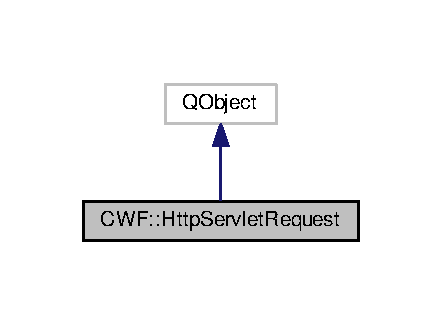
\includegraphics[width=212pt]{class_c_w_f_1_1_http_servlet_request__inherit__graph}
\end{center}
\end{figure}
\subsection*{Public Member Functions}
\begin{DoxyCompactItemize}
\item 
\hyperlink{class_c_w_f_1_1_http_servlet_request_a9fdd1aeaccd42c3043bff902cf6e6e09}{Http\+Servlet\+Request} (Q\+Tcp\+Socket \&socket, const Q\+String \&path, const Q\+String \&suffix)
\begin{DoxyCompactList}\small\item\em This constructor needs to receive a reference to a Q\+Tcp\+Socket and Q\+Byte\+Array. The parameter parent is optional. N\+O\+T\+E\+: The \hyperlink{class_c_w_f_1_1_cpp_web_server}{Cpp\+Web\+Server} is responsable to create the Q\+Tcp\+Socket, and the \hyperlink{class_c_w_f_1_1_http_read_request}{Http\+Read\+Request} is responsable to create a \hyperlink{class_c_w_f_1_1_http_read_request}{Http\+Read\+Request} and a \hyperlink{class_c_w_f_1_1_http_servlet_response}{Http\+Servlet\+Response}. \end{DoxyCompactList}\item 
virtual \hyperlink{class_c_w_f_1_1_http_servlet_request_a41867870bf0c9f23ef74d70b10c0d357}{$\sim$\+Http\+Servlet\+Request} ()
\begin{DoxyCompactList}\small\item\em Destructor. \end{DoxyCompactList}\item 
void \hyperlink{class_c_w_f_1_1_http_servlet_request_ad4777049d7043e62535fa658fd61be1d}{add\+Attribute} (const Q\+String \&name, Q\+Object $\ast$value)
\begin{DoxyCompactList}\small\item\em This method add an attribute that will be passed to a xhtml page. \end{DoxyCompactList}\item 
Q\+Map$<$ Q\+String, Q\+Object $\ast$ $>$ \hyperlink{class_c_w_f_1_1_http_servlet_request_a3855042c53725e7ef753bee620e01297}{get\+Attributes} () const 
\begin{DoxyCompactList}\small\item\em This method returns all the attributes of a \hyperlink{class_c_w_f_1_1_http_read_request}{Http\+Read\+Request}. \end{DoxyCompactList}\item 
const Q\+Object $\ast$ \hyperlink{class_c_w_f_1_1_http_servlet_request_a6833f3628440cfa4a6dc45fcd6783eee}{get\+Attribute} (const Q\+String \&name) const 
\begin{DoxyCompactList}\small\item\em This method returns a specific object given its name. \end{DoxyCompactList}\item 
const Q\+Byte\+Array \hyperlink{class_c_w_f_1_1_http_servlet_request_a9b46d51ca2410ec587f980fc86d75027}{get\+Body} () const 
\item 
\hyperlink{class_c_w_f_1_1_request_dispatcher}{Request\+Dispatcher} \& \hyperlink{class_c_w_f_1_1_http_servlet_request_a0ce93d793a178c7e0e5fef4044b48bdc}{get\+Request\+Dispatcher} (const Q\+String \&page)
\begin{DoxyCompactList}\small\item\em This method returns a request\+Dispatcher given an specific page. \end{DoxyCompactList}\item 
Q\+Byte\+Array \hyperlink{class_c_w_f_1_1_http_servlet_request_a487fd95aa9c7f64cfa438097a59a30ca}{get\+Protocol} () const 
\begin{DoxyCompactList}\small\item\em This method returns the http protocol. \end{DoxyCompactList}\item 
void \hyperlink{class_c_w_f_1_1_http_servlet_request_a1e17ba223b17b4b390c9a351d4fff78e}{clear\+Attributes} ()
\begin{DoxyCompactList}\small\item\em This method will clear all the attributes. \end{DoxyCompactList}\item 
void \hyperlink{class_c_w_f_1_1_http_servlet_request_a0c28aa6bbd0cf10b482098c70fe2c0fd}{set\+Http\+Parser} (\hyperlink{class_c_w_f_1_1_http_parser}{Http\+Parser} \&http\+Parser)
\begin{DoxyCompactList}\small\item\em This method set the \hyperlink{class_c_w_f_1_1_http_parser}{Http\+Parser}. \end{DoxyCompactList}\item 
\hyperlink{class_c_w_f_1_1_http_parser}{Http\+Parser} \& \hyperlink{class_c_w_f_1_1_http_servlet_request_a3bb5c268aecca784c632c673078b4150}{get\+Http\+Parser} () const 
\begin{DoxyCompactList}\small\item\em This method returns the \hyperlink{class_c_w_f_1_1_http_parser}{Http\+Parser}. \end{DoxyCompactList}\item 
Q\+Byte\+Array \hyperlink{class_c_w_f_1_1_http_servlet_request_a9408f2866aa0fc49242e74b85a514869}{get\+Request\+U\+R\+L} () const 
\begin{DoxyCompactList}\small\item\em This method returns the requested url. \end{DoxyCompactList}\item 
Q\+Byte\+Array \hyperlink{class_c_w_f_1_1_http_servlet_request_ade6b21cdd789a5892e472915ede386fd}{get\+Request\+U\+R\+I} () const 
\begin{DoxyCompactList}\small\item\em This method returns the requested url. \end{DoxyCompactList}\item 
\hyperlink{class_c_w_f_1_1_http_session}{Http\+Session} \& \hyperlink{class_c_w_f_1_1_http_servlet_request_aad0cadb7d24101705a6f83b82eb7c025}{get\+Session} () const 
\begin{DoxyCompactList}\small\item\em This method returns the user's session. \end{DoxyCompactList}\item 
void \hyperlink{class_c_w_f_1_1_http_servlet_request_a2a613871d53495a3bacb61d68a424708}{set\+Session} (\hyperlink{class_c_w_f_1_1_http_session}{Http\+Session} \&session)
\begin{DoxyCompactList}\small\item\em This method set the user's session. \end{DoxyCompactList}\item 
Q\+Byte\+Array \hyperlink{class_c_w_f_1_1_http_servlet_request_a09c2b6f6241263a2626686e80ab6e126}{get\+Parameter} (const Q\+Byte\+Array \&name) const 
\begin{DoxyCompactList}\small\item\em This method returns the most recent parameter from a request given an specific name. \end{DoxyCompactList}\item 
Q\+Byte\+Array\+List \hyperlink{class_c_w_f_1_1_http_servlet_request_afc56e6e1a1d76c727924de6847c4ef27}{get\+Parameters} (const Q\+Byte\+Array \&name) const 
\begin{DoxyCompactList}\small\item\em This method returns the parameters from a request given an specific name. \end{DoxyCompactList}\item 
Q\+Tcp\+Socket \& \hyperlink{class_c_w_f_1_1_http_servlet_request_ad6496a8dcda50dd7ec9f389b4cbb4349}{get\+Socket} () const 
\begin{DoxyCompactList}\small\item\em This method returns a reference to the current socket. \end{DoxyCompactList}\item 
bool \hyperlink{class_c_w_f_1_1_http_servlet_request_abe9c009a7010f02552da1370dddd0484}{get\+Auto\+Delete\+Attribute} () const 
\begin{DoxyCompactList}\small\item\em This method returns the auto delete attribute. \end{DoxyCompactList}\item 
void \hyperlink{class_c_w_f_1_1_http_servlet_request_a4f884f904ea3793511087b6311fb9e47}{set\+Auto\+Delete\+Attribute} (bool value)
\begin{DoxyCompactList}\small\item\em This method sets the auto delete attribute. When the auto delete attribute is true and the \hyperlink{class_c_w_f_1_1_http_servlet_request}{Http\+Servlet\+Request} is destroyed, the attributes that you added will be destroyed. N\+O\+T\+E\+: By default the auto delete attribute is false. \end{DoxyCompactList}\item 
Q\+String \hyperlink{class_c_w_f_1_1_http_servlet_request_ad26dd1fc71d21453fc0e28ab602f9603}{get\+Path} () const 
\begin{DoxyCompactList}\small\item\em This method returns the path. \end{DoxyCompactList}\item 
Q\+Multi\+Map$<$ Q\+Byte\+Array, Q\+Byte\+Array $>$ \hyperlink{class_c_w_f_1_1_http_servlet_request_a67e5b7ef1e55618ff787ab3d5e229246}{get\+Uploaded\+Files} () const 
\begin{DoxyCompactList}\small\item\em This method returns all the files that the user has sent. \end{DoxyCompactList}\item 
void \hyperlink{class_c_w_f_1_1_http_servlet_request_a82a05ddb8d91c72a28846ffc0e811ee7}{fill\+Q\+Object} (Q\+Object $\ast$object)
\end{DoxyCompactItemize}
\subsection*{Friends}
\begin{DoxyCompactItemize}
\item 
class \hyperlink{class_c_w_f_1_1_http_servlet_request_a4d54f5003e07e218070a449c22a52c7c}{Http\+Read\+Request}
\item 
class \hyperlink{class_c_w_f_1_1_http_servlet_request_ae82f2dbbf52e70637edba766141fd80e}{Request\+Dispatcher}
\end{DoxyCompactItemize}


\subsection{Detailed Description}
The \hyperlink{class_c_w_f_1_1_http_servlet_request}{Http\+Servlet\+Request} class holds all information about a http request. 

\subsection{Constructor \& Destructor Documentation}
\hypertarget{class_c_w_f_1_1_http_servlet_request_a9fdd1aeaccd42c3043bff902cf6e6e09}{\index{C\+W\+F\+::\+Http\+Servlet\+Request@{C\+W\+F\+::\+Http\+Servlet\+Request}!Http\+Servlet\+Request@{Http\+Servlet\+Request}}
\index{Http\+Servlet\+Request@{Http\+Servlet\+Request}!C\+W\+F\+::\+Http\+Servlet\+Request@{C\+W\+F\+::\+Http\+Servlet\+Request}}
\subsubsection[{Http\+Servlet\+Request}]{\setlength{\rightskip}{0pt plus 5cm}C\+W\+F\+::\+Http\+Servlet\+Request\+::\+Http\+Servlet\+Request (
\begin{DoxyParamCaption}
\item[{Q\+Tcp\+Socket \&}]{socket, }
\item[{const Q\+String \&}]{path, }
\item[{const Q\+String \&}]{suffix}
\end{DoxyParamCaption}
)\hspace{0.3cm}{\ttfamily [explicit]}}}\label{class_c_w_f_1_1_http_servlet_request_a9fdd1aeaccd42c3043bff902cf6e6e09}


This constructor needs to receive a reference to a Q\+Tcp\+Socket and Q\+Byte\+Array. The parameter parent is optional. N\+O\+T\+E\+: The \hyperlink{class_c_w_f_1_1_cpp_web_server}{Cpp\+Web\+Server} is responsable to create the Q\+Tcp\+Socket, and the \hyperlink{class_c_w_f_1_1_http_read_request}{Http\+Read\+Request} is responsable to create a \hyperlink{class_c_w_f_1_1_http_read_request}{Http\+Read\+Request} and a \hyperlink{class_c_w_f_1_1_http_servlet_response}{Http\+Servlet\+Response}. 


\begin{DoxyParams}{Parameters}
{\em socket} & \+: This is a reference to a Q\+Tcp\+Socket. \\
\hline
{\em path} & \+: This is a reference to a Q\+Byte\+Array. \\
\hline
{\em parent} & \+: This is a pointer to a Q\+Object. \\
\hline
\end{DoxyParams}
\hypertarget{class_c_w_f_1_1_http_servlet_request_a41867870bf0c9f23ef74d70b10c0d357}{\index{C\+W\+F\+::\+Http\+Servlet\+Request@{C\+W\+F\+::\+Http\+Servlet\+Request}!````~Http\+Servlet\+Request@{$\sim$\+Http\+Servlet\+Request}}
\index{````~Http\+Servlet\+Request@{$\sim$\+Http\+Servlet\+Request}!C\+W\+F\+::\+Http\+Servlet\+Request@{C\+W\+F\+::\+Http\+Servlet\+Request}}
\subsubsection[{$\sim$\+Http\+Servlet\+Request}]{\setlength{\rightskip}{0pt plus 5cm}C\+W\+F\+::\+Http\+Servlet\+Request\+::$\sim$\+Http\+Servlet\+Request (
\begin{DoxyParamCaption}
{}
\end{DoxyParamCaption}
)\hspace{0.3cm}{\ttfamily [virtual]}}}\label{class_c_w_f_1_1_http_servlet_request_a41867870bf0c9f23ef74d70b10c0d357}


Destructor. 



\subsection{Member Function Documentation}
\hypertarget{class_c_w_f_1_1_http_servlet_request_ad4777049d7043e62535fa658fd61be1d}{\index{C\+W\+F\+::\+Http\+Servlet\+Request@{C\+W\+F\+::\+Http\+Servlet\+Request}!add\+Attribute@{add\+Attribute}}
\index{add\+Attribute@{add\+Attribute}!C\+W\+F\+::\+Http\+Servlet\+Request@{C\+W\+F\+::\+Http\+Servlet\+Request}}
\subsubsection[{add\+Attribute}]{\setlength{\rightskip}{0pt plus 5cm}void C\+W\+F\+::\+Http\+Servlet\+Request\+::add\+Attribute (
\begin{DoxyParamCaption}
\item[{const Q\+String \&}]{name, }
\item[{Q\+Object $\ast$}]{value}
\end{DoxyParamCaption}
)}}\label{class_c_w_f_1_1_http_servlet_request_ad4777049d7043e62535fa658fd61be1d}


This method add an attribute that will be passed to a xhtml page. 


\begin{DoxyParams}{Parameters}
{\em path} & \+: This is a reference to a Q\+Byte\+Array and holds a name of a object that will be used in a xhtml page. \\
\hline
{\em value} & \+: This is a pointer to a Q\+Object and holds the object that will be used by the \hyperlink{class_c_w_f_1_1_c_s_t_l_compiler}{C\+S\+T\+L\+Compiler} to process a xhtml page and generates its output. \\
\hline
\end{DoxyParams}
\hypertarget{class_c_w_f_1_1_http_servlet_request_a1e17ba223b17b4b390c9a351d4fff78e}{\index{C\+W\+F\+::\+Http\+Servlet\+Request@{C\+W\+F\+::\+Http\+Servlet\+Request}!clear\+Attributes@{clear\+Attributes}}
\index{clear\+Attributes@{clear\+Attributes}!C\+W\+F\+::\+Http\+Servlet\+Request@{C\+W\+F\+::\+Http\+Servlet\+Request}}
\subsubsection[{clear\+Attributes}]{\setlength{\rightskip}{0pt plus 5cm}void C\+W\+F\+::\+Http\+Servlet\+Request\+::clear\+Attributes (
\begin{DoxyParamCaption}
{}
\end{DoxyParamCaption}
)}}\label{class_c_w_f_1_1_http_servlet_request_a1e17ba223b17b4b390c9a351d4fff78e}


This method will clear all the attributes. 

\hypertarget{class_c_w_f_1_1_http_servlet_request_a82a05ddb8d91c72a28846ffc0e811ee7}{\index{C\+W\+F\+::\+Http\+Servlet\+Request@{C\+W\+F\+::\+Http\+Servlet\+Request}!fill\+Q\+Object@{fill\+Q\+Object}}
\index{fill\+Q\+Object@{fill\+Q\+Object}!C\+W\+F\+::\+Http\+Servlet\+Request@{C\+W\+F\+::\+Http\+Servlet\+Request}}
\subsubsection[{fill\+Q\+Object}]{\setlength{\rightskip}{0pt plus 5cm}void C\+W\+F\+::\+Http\+Servlet\+Request\+::fill\+Q\+Object (
\begin{DoxyParamCaption}
\item[{Q\+Object $\ast$}]{object}
\end{DoxyParamCaption}
)}}\label{class_c_w_f_1_1_http_servlet_request_a82a05ddb8d91c72a28846ffc0e811ee7}
\hypertarget{class_c_w_f_1_1_http_servlet_request_a6833f3628440cfa4a6dc45fcd6783eee}{\index{C\+W\+F\+::\+Http\+Servlet\+Request@{C\+W\+F\+::\+Http\+Servlet\+Request}!get\+Attribute@{get\+Attribute}}
\index{get\+Attribute@{get\+Attribute}!C\+W\+F\+::\+Http\+Servlet\+Request@{C\+W\+F\+::\+Http\+Servlet\+Request}}
\subsubsection[{get\+Attribute}]{\setlength{\rightskip}{0pt plus 5cm}const Q\+Object $\ast$ C\+W\+F\+::\+Http\+Servlet\+Request\+::get\+Attribute (
\begin{DoxyParamCaption}
\item[{const Q\+String \&}]{name}
\end{DoxyParamCaption}
) const}}\label{class_c_w_f_1_1_http_servlet_request_a6833f3628440cfa4a6dc45fcd6783eee}


This method returns a specific object given its name. 


\begin{DoxyParams}{Parameters}
{\em name} & \+: This is a reference to a Q\+Byte\+Array. \\
\hline
\end{DoxyParams}
\begin{DoxyReturn}{Returns}
const Q\+Object $\ast$ 
\end{DoxyReturn}
\hypertarget{class_c_w_f_1_1_http_servlet_request_a3855042c53725e7ef753bee620e01297}{\index{C\+W\+F\+::\+Http\+Servlet\+Request@{C\+W\+F\+::\+Http\+Servlet\+Request}!get\+Attributes@{get\+Attributes}}
\index{get\+Attributes@{get\+Attributes}!C\+W\+F\+::\+Http\+Servlet\+Request@{C\+W\+F\+::\+Http\+Servlet\+Request}}
\subsubsection[{get\+Attributes}]{\setlength{\rightskip}{0pt plus 5cm}Q\+Map$<$ Q\+String, Q\+Object $\ast$ $>$ C\+W\+F\+::\+Http\+Servlet\+Request\+::get\+Attributes (
\begin{DoxyParamCaption}
{}
\end{DoxyParamCaption}
) const}}\label{class_c_w_f_1_1_http_servlet_request_a3855042c53725e7ef753bee620e01297}


This method returns all the attributes of a \hyperlink{class_c_w_f_1_1_http_read_request}{Http\+Read\+Request}. 

\begin{DoxyReturn}{Returns}
Q\+Map$<$\+Q\+Byte\+Array, Q\+Object $\ast$$>$ 
\end{DoxyReturn}
\hypertarget{class_c_w_f_1_1_http_servlet_request_abe9c009a7010f02552da1370dddd0484}{\index{C\+W\+F\+::\+Http\+Servlet\+Request@{C\+W\+F\+::\+Http\+Servlet\+Request}!get\+Auto\+Delete\+Attribute@{get\+Auto\+Delete\+Attribute}}
\index{get\+Auto\+Delete\+Attribute@{get\+Auto\+Delete\+Attribute}!C\+W\+F\+::\+Http\+Servlet\+Request@{C\+W\+F\+::\+Http\+Servlet\+Request}}
\subsubsection[{get\+Auto\+Delete\+Attribute}]{\setlength{\rightskip}{0pt plus 5cm}bool C\+W\+F\+::\+Http\+Servlet\+Request\+::get\+Auto\+Delete\+Attribute (
\begin{DoxyParamCaption}
{}
\end{DoxyParamCaption}
) const}}\label{class_c_w_f_1_1_http_servlet_request_abe9c009a7010f02552da1370dddd0484}


This method returns the auto delete attribute. 

\begin{DoxyReturn}{Returns}
bool 
\end{DoxyReturn}
\hypertarget{class_c_w_f_1_1_http_servlet_request_a9b46d51ca2410ec587f980fc86d75027}{\index{C\+W\+F\+::\+Http\+Servlet\+Request@{C\+W\+F\+::\+Http\+Servlet\+Request}!get\+Body@{get\+Body}}
\index{get\+Body@{get\+Body}!C\+W\+F\+::\+Http\+Servlet\+Request@{C\+W\+F\+::\+Http\+Servlet\+Request}}
\subsubsection[{get\+Body}]{\setlength{\rightskip}{0pt plus 5cm}const Q\+Byte\+Array C\+W\+F\+::\+Http\+Servlet\+Request\+::get\+Body (
\begin{DoxyParamCaption}
{}
\end{DoxyParamCaption}
) const}}\label{class_c_w_f_1_1_http_servlet_request_a9b46d51ca2410ec587f980fc86d75027}
\hypertarget{class_c_w_f_1_1_http_servlet_request_a3bb5c268aecca784c632c673078b4150}{\index{C\+W\+F\+::\+Http\+Servlet\+Request@{C\+W\+F\+::\+Http\+Servlet\+Request}!get\+Http\+Parser@{get\+Http\+Parser}}
\index{get\+Http\+Parser@{get\+Http\+Parser}!C\+W\+F\+::\+Http\+Servlet\+Request@{C\+W\+F\+::\+Http\+Servlet\+Request}}
\subsubsection[{get\+Http\+Parser}]{\setlength{\rightskip}{0pt plus 5cm}{\bf Http\+Parser} \& C\+W\+F\+::\+Http\+Servlet\+Request\+::get\+Http\+Parser (
\begin{DoxyParamCaption}
{}
\end{DoxyParamCaption}
) const}}\label{class_c_w_f_1_1_http_servlet_request_a3bb5c268aecca784c632c673078b4150}


This method returns the \hyperlink{class_c_w_f_1_1_http_parser}{Http\+Parser}. 

\begin{DoxyReturn}{Returns}
\hyperlink{class_c_w_f_1_1_http_parser}{Http\+Parser} 
\end{DoxyReturn}
\hypertarget{class_c_w_f_1_1_http_servlet_request_a09c2b6f6241263a2626686e80ab6e126}{\index{C\+W\+F\+::\+Http\+Servlet\+Request@{C\+W\+F\+::\+Http\+Servlet\+Request}!get\+Parameter@{get\+Parameter}}
\index{get\+Parameter@{get\+Parameter}!C\+W\+F\+::\+Http\+Servlet\+Request@{C\+W\+F\+::\+Http\+Servlet\+Request}}
\subsubsection[{get\+Parameter}]{\setlength{\rightskip}{0pt plus 5cm}Q\+Byte\+Array C\+W\+F\+::\+Http\+Servlet\+Request\+::get\+Parameter (
\begin{DoxyParamCaption}
\item[{const Q\+Byte\+Array \&}]{name}
\end{DoxyParamCaption}
) const}}\label{class_c_w_f_1_1_http_servlet_request_a09c2b6f6241263a2626686e80ab6e126}


This method returns the most recent parameter from a request given an specific name. 


\begin{DoxyParams}{Parameters}
{\em name} & \+: This is a reference to a Q\+Byte\+Array. \\
\hline
\end{DoxyParams}
\begin{DoxyReturn}{Returns}
Q\+Byte\+Array 
\end{DoxyReturn}
\hypertarget{class_c_w_f_1_1_http_servlet_request_afc56e6e1a1d76c727924de6847c4ef27}{\index{C\+W\+F\+::\+Http\+Servlet\+Request@{C\+W\+F\+::\+Http\+Servlet\+Request}!get\+Parameters@{get\+Parameters}}
\index{get\+Parameters@{get\+Parameters}!C\+W\+F\+::\+Http\+Servlet\+Request@{C\+W\+F\+::\+Http\+Servlet\+Request}}
\subsubsection[{get\+Parameters}]{\setlength{\rightskip}{0pt plus 5cm}Q\+Byte\+Array\+List C\+W\+F\+::\+Http\+Servlet\+Request\+::get\+Parameters (
\begin{DoxyParamCaption}
\item[{const Q\+Byte\+Array \&}]{name}
\end{DoxyParamCaption}
) const}}\label{class_c_w_f_1_1_http_servlet_request_afc56e6e1a1d76c727924de6847c4ef27}


This method returns the parameters from a request given an specific name. 


\begin{DoxyParams}{Parameters}
{\em name} & \+: This is a reference to a Q\+Byte\+Array. \\
\hline
\end{DoxyParams}
\begin{DoxyReturn}{Returns}
Q\+Byte\+Array 
\end{DoxyReturn}
\hypertarget{class_c_w_f_1_1_http_servlet_request_ad26dd1fc71d21453fc0e28ab602f9603}{\index{C\+W\+F\+::\+Http\+Servlet\+Request@{C\+W\+F\+::\+Http\+Servlet\+Request}!get\+Path@{get\+Path}}
\index{get\+Path@{get\+Path}!C\+W\+F\+::\+Http\+Servlet\+Request@{C\+W\+F\+::\+Http\+Servlet\+Request}}
\subsubsection[{get\+Path}]{\setlength{\rightskip}{0pt plus 5cm}Q\+String C\+W\+F\+::\+Http\+Servlet\+Request\+::get\+Path (
\begin{DoxyParamCaption}
{}
\end{DoxyParamCaption}
) const}}\label{class_c_w_f_1_1_http_servlet_request_ad26dd1fc71d21453fc0e28ab602f9603}


This method returns the path. 

\begin{DoxyReturn}{Returns}
Q\+String 
\end{DoxyReturn}
\hypertarget{class_c_w_f_1_1_http_servlet_request_a487fd95aa9c7f64cfa438097a59a30ca}{\index{C\+W\+F\+::\+Http\+Servlet\+Request@{C\+W\+F\+::\+Http\+Servlet\+Request}!get\+Protocol@{get\+Protocol}}
\index{get\+Protocol@{get\+Protocol}!C\+W\+F\+::\+Http\+Servlet\+Request@{C\+W\+F\+::\+Http\+Servlet\+Request}}
\subsubsection[{get\+Protocol}]{\setlength{\rightskip}{0pt plus 5cm}Q\+Byte\+Array C\+W\+F\+::\+Http\+Servlet\+Request\+::get\+Protocol (
\begin{DoxyParamCaption}
{}
\end{DoxyParamCaption}
) const}}\label{class_c_w_f_1_1_http_servlet_request_a487fd95aa9c7f64cfa438097a59a30ca}


This method returns the http protocol. 

\begin{DoxyReturn}{Returns}
Q\+Byte\+Array 
\end{DoxyReturn}
\hypertarget{class_c_w_f_1_1_http_servlet_request_a0ce93d793a178c7e0e5fef4044b48bdc}{\index{C\+W\+F\+::\+Http\+Servlet\+Request@{C\+W\+F\+::\+Http\+Servlet\+Request}!get\+Request\+Dispatcher@{get\+Request\+Dispatcher}}
\index{get\+Request\+Dispatcher@{get\+Request\+Dispatcher}!C\+W\+F\+::\+Http\+Servlet\+Request@{C\+W\+F\+::\+Http\+Servlet\+Request}}
\subsubsection[{get\+Request\+Dispatcher}]{\setlength{\rightskip}{0pt plus 5cm}{\bf Request\+Dispatcher} \& C\+W\+F\+::\+Http\+Servlet\+Request\+::get\+Request\+Dispatcher (
\begin{DoxyParamCaption}
\item[{const Q\+String \&}]{page}
\end{DoxyParamCaption}
)}}\label{class_c_w_f_1_1_http_servlet_request_a0ce93d793a178c7e0e5fef4044b48bdc}


This method returns a request\+Dispatcher given an specific page. 


\begin{DoxyParams}{Parameters}
{\em page} & \+: This is a reference to a Q\+Byte\+Array. \\
\hline
\end{DoxyParams}
\begin{DoxyReturn}{Returns}
\hyperlink{class_c_w_f_1_1_request_dispatcher}{Request\+Dispatcher} 
\end{DoxyReturn}
\hypertarget{class_c_w_f_1_1_http_servlet_request_ade6b21cdd789a5892e472915ede386fd}{\index{C\+W\+F\+::\+Http\+Servlet\+Request@{C\+W\+F\+::\+Http\+Servlet\+Request}!get\+Request\+U\+R\+I@{get\+Request\+U\+R\+I}}
\index{get\+Request\+U\+R\+I@{get\+Request\+U\+R\+I}!C\+W\+F\+::\+Http\+Servlet\+Request@{C\+W\+F\+::\+Http\+Servlet\+Request}}
\subsubsection[{get\+Request\+U\+R\+I}]{\setlength{\rightskip}{0pt plus 5cm}Q\+Byte\+Array C\+W\+F\+::\+Http\+Servlet\+Request\+::get\+Request\+U\+R\+I (
\begin{DoxyParamCaption}
{}
\end{DoxyParamCaption}
) const}}\label{class_c_w_f_1_1_http_servlet_request_ade6b21cdd789a5892e472915ede386fd}


This method returns the requested url. 

\begin{DoxyReturn}{Returns}
Q\+Byte\+Array 
\end{DoxyReturn}
\hypertarget{class_c_w_f_1_1_http_servlet_request_a9408f2866aa0fc49242e74b85a514869}{\index{C\+W\+F\+::\+Http\+Servlet\+Request@{C\+W\+F\+::\+Http\+Servlet\+Request}!get\+Request\+U\+R\+L@{get\+Request\+U\+R\+L}}
\index{get\+Request\+U\+R\+L@{get\+Request\+U\+R\+L}!C\+W\+F\+::\+Http\+Servlet\+Request@{C\+W\+F\+::\+Http\+Servlet\+Request}}
\subsubsection[{get\+Request\+U\+R\+L}]{\setlength{\rightskip}{0pt plus 5cm}Q\+Byte\+Array C\+W\+F\+::\+Http\+Servlet\+Request\+::get\+Request\+U\+R\+L (
\begin{DoxyParamCaption}
{}
\end{DoxyParamCaption}
) const}}\label{class_c_w_f_1_1_http_servlet_request_a9408f2866aa0fc49242e74b85a514869}


This method returns the requested url. 

\begin{DoxyReturn}{Returns}
Q\+Byte\+Array 
\end{DoxyReturn}
\hypertarget{class_c_w_f_1_1_http_servlet_request_aad0cadb7d24101705a6f83b82eb7c025}{\index{C\+W\+F\+::\+Http\+Servlet\+Request@{C\+W\+F\+::\+Http\+Servlet\+Request}!get\+Session@{get\+Session}}
\index{get\+Session@{get\+Session}!C\+W\+F\+::\+Http\+Servlet\+Request@{C\+W\+F\+::\+Http\+Servlet\+Request}}
\subsubsection[{get\+Session}]{\setlength{\rightskip}{0pt plus 5cm}{\bf Http\+Session} \& C\+W\+F\+::\+Http\+Servlet\+Request\+::get\+Session (
\begin{DoxyParamCaption}
{}
\end{DoxyParamCaption}
) const}}\label{class_c_w_f_1_1_http_servlet_request_aad0cadb7d24101705a6f83b82eb7c025}


This method returns the user's session. 

\hypertarget{class_c_w_f_1_1_http_servlet_request_ad6496a8dcda50dd7ec9f389b4cbb4349}{\index{C\+W\+F\+::\+Http\+Servlet\+Request@{C\+W\+F\+::\+Http\+Servlet\+Request}!get\+Socket@{get\+Socket}}
\index{get\+Socket@{get\+Socket}!C\+W\+F\+::\+Http\+Servlet\+Request@{C\+W\+F\+::\+Http\+Servlet\+Request}}
\subsubsection[{get\+Socket}]{\setlength{\rightskip}{0pt plus 5cm}Q\+Tcp\+Socket \& C\+W\+F\+::\+Http\+Servlet\+Request\+::get\+Socket (
\begin{DoxyParamCaption}
{}
\end{DoxyParamCaption}
) const}}\label{class_c_w_f_1_1_http_servlet_request_ad6496a8dcda50dd7ec9f389b4cbb4349}


This method returns a reference to the current socket. 

\begin{DoxyReturn}{Returns}
Q\+Tcp\+Socket 
\end{DoxyReturn}
\hypertarget{class_c_w_f_1_1_http_servlet_request_a67e5b7ef1e55618ff787ab3d5e229246}{\index{C\+W\+F\+::\+Http\+Servlet\+Request@{C\+W\+F\+::\+Http\+Servlet\+Request}!get\+Uploaded\+Files@{get\+Uploaded\+Files}}
\index{get\+Uploaded\+Files@{get\+Uploaded\+Files}!C\+W\+F\+::\+Http\+Servlet\+Request@{C\+W\+F\+::\+Http\+Servlet\+Request}}
\subsubsection[{get\+Uploaded\+Files}]{\setlength{\rightskip}{0pt plus 5cm}Q\+Multi\+Map$<$ Q\+Byte\+Array, Q\+Byte\+Array $>$ C\+W\+F\+::\+Http\+Servlet\+Request\+::get\+Uploaded\+Files (
\begin{DoxyParamCaption}
{}
\end{DoxyParamCaption}
) const}}\label{class_c_w_f_1_1_http_servlet_request_a67e5b7ef1e55618ff787ab3d5e229246}


This method returns all the files that the user has sent. 

\begin{DoxyReturn}{Returns}
Q\+Map$<$\+Q\+Byte\+Array, Q\+Byte\+Array$>$ 
\end{DoxyReturn}
\hypertarget{class_c_w_f_1_1_http_servlet_request_a4f884f904ea3793511087b6311fb9e47}{\index{C\+W\+F\+::\+Http\+Servlet\+Request@{C\+W\+F\+::\+Http\+Servlet\+Request}!set\+Auto\+Delete\+Attribute@{set\+Auto\+Delete\+Attribute}}
\index{set\+Auto\+Delete\+Attribute@{set\+Auto\+Delete\+Attribute}!C\+W\+F\+::\+Http\+Servlet\+Request@{C\+W\+F\+::\+Http\+Servlet\+Request}}
\subsubsection[{set\+Auto\+Delete\+Attribute}]{\setlength{\rightskip}{0pt plus 5cm}void C\+W\+F\+::\+Http\+Servlet\+Request\+::set\+Auto\+Delete\+Attribute (
\begin{DoxyParamCaption}
\item[{bool}]{value}
\end{DoxyParamCaption}
)}}\label{class_c_w_f_1_1_http_servlet_request_a4f884f904ea3793511087b6311fb9e47}


This method sets the auto delete attribute. When the auto delete attribute is true and the \hyperlink{class_c_w_f_1_1_http_servlet_request}{Http\+Servlet\+Request} is destroyed, the attributes that you added will be destroyed. N\+O\+T\+E\+: By default the auto delete attribute is false. 


\begin{DoxyParams}{Parameters}
{\em value} & \+: This sets the auto delete attribute. \\
\hline
\end{DoxyParams}
\hypertarget{class_c_w_f_1_1_http_servlet_request_a0c28aa6bbd0cf10b482098c70fe2c0fd}{\index{C\+W\+F\+::\+Http\+Servlet\+Request@{C\+W\+F\+::\+Http\+Servlet\+Request}!set\+Http\+Parser@{set\+Http\+Parser}}
\index{set\+Http\+Parser@{set\+Http\+Parser}!C\+W\+F\+::\+Http\+Servlet\+Request@{C\+W\+F\+::\+Http\+Servlet\+Request}}
\subsubsection[{set\+Http\+Parser}]{\setlength{\rightskip}{0pt plus 5cm}void C\+W\+F\+::\+Http\+Servlet\+Request\+::set\+Http\+Parser (
\begin{DoxyParamCaption}
\item[{{\bf Http\+Parser} \&}]{http\+Parser}
\end{DoxyParamCaption}
)}}\label{class_c_w_f_1_1_http_servlet_request_a0c28aa6bbd0cf10b482098c70fe2c0fd}


This method set the \hyperlink{class_c_w_f_1_1_http_parser}{Http\+Parser}. 


\begin{DoxyParams}{Parameters}
{\em http\+Parser} & \\
\hline
\end{DoxyParams}
\hypertarget{class_c_w_f_1_1_http_servlet_request_a2a613871d53495a3bacb61d68a424708}{\index{C\+W\+F\+::\+Http\+Servlet\+Request@{C\+W\+F\+::\+Http\+Servlet\+Request}!set\+Session@{set\+Session}}
\index{set\+Session@{set\+Session}!C\+W\+F\+::\+Http\+Servlet\+Request@{C\+W\+F\+::\+Http\+Servlet\+Request}}
\subsubsection[{set\+Session}]{\setlength{\rightskip}{0pt plus 5cm}void C\+W\+F\+::\+Http\+Servlet\+Request\+::set\+Session (
\begin{DoxyParamCaption}
\item[{{\bf Http\+Session} \&}]{session}
\end{DoxyParamCaption}
)}}\label{class_c_w_f_1_1_http_servlet_request_a2a613871d53495a3bacb61d68a424708}


This method set the user's session. 

\begin{DoxyReturn}{Returns}
\hyperlink{class_c_w_f_1_1_http_session}{Http\+Session} 
\end{DoxyReturn}


\subsection{Friends And Related Function Documentation}
\hypertarget{class_c_w_f_1_1_http_servlet_request_a4d54f5003e07e218070a449c22a52c7c}{\index{C\+W\+F\+::\+Http\+Servlet\+Request@{C\+W\+F\+::\+Http\+Servlet\+Request}!Http\+Read\+Request@{Http\+Read\+Request}}
\index{Http\+Read\+Request@{Http\+Read\+Request}!C\+W\+F\+::\+Http\+Servlet\+Request@{C\+W\+F\+::\+Http\+Servlet\+Request}}
\subsubsection[{Http\+Read\+Request}]{\setlength{\rightskip}{0pt plus 5cm}friend class {\bf Http\+Read\+Request}\hspace{0.3cm}{\ttfamily [friend]}}}\label{class_c_w_f_1_1_http_servlet_request_a4d54f5003e07e218070a449c22a52c7c}
\hypertarget{class_c_w_f_1_1_http_servlet_request_ae82f2dbbf52e70637edba766141fd80e}{\index{C\+W\+F\+::\+Http\+Servlet\+Request@{C\+W\+F\+::\+Http\+Servlet\+Request}!Request\+Dispatcher@{Request\+Dispatcher}}
\index{Request\+Dispatcher@{Request\+Dispatcher}!C\+W\+F\+::\+Http\+Servlet\+Request@{C\+W\+F\+::\+Http\+Servlet\+Request}}
\subsubsection[{Request\+Dispatcher}]{\setlength{\rightskip}{0pt plus 5cm}friend class {\bf Request\+Dispatcher}\hspace{0.3cm}{\ttfamily [friend]}}}\label{class_c_w_f_1_1_http_servlet_request_ae82f2dbbf52e70637edba766141fd80e}


The documentation for this class was generated from the following files\+:\begin{DoxyCompactItemize}
\item 
/home/herik/\+C\+P\+P\+Web\+Framework/\+C\+P\+P\+Web\+Framework/cwf/\hyperlink{httpservletrequest_8h}{httpservletrequest.\+h}\item 
/home/herik/\+C\+P\+P\+Web\+Framework/\+C\+P\+P\+Web\+Framework/cwf/\hyperlink{httpservletrequest_8cpp}{httpservletrequest.\+cpp}\end{DoxyCompactItemize}

\hypertarget{class_c_w_f_1_1_http_servlet_response}{\section{C\+W\+F\+:\+:Http\+Servlet\+Response Class Reference}
\label{class_c_w_f_1_1_http_servlet_response}\index{C\+W\+F\+::\+Http\+Servlet\+Response@{C\+W\+F\+::\+Http\+Servlet\+Response}}
}


The \hyperlink{class_c_w_f_1_1_http_servlet_response}{Http\+Servlet\+Response} class is responsable to response a Http request.  




{\ttfamily \#include $<$httpservletresponse.\+h$>$}

\subsection*{Public Member Functions}
\begin{DoxyCompactItemize}
\item 
\hyperlink{class_c_w_f_1_1_http_servlet_response_a5c89f340f44874457e680b02ab31d290}{Http\+Servlet\+Response} (Q\+Tcp\+Socket \&socket)
\item 
virtual \hyperlink{class_c_w_f_1_1_http_servlet_response_a2081a62779b85a5805812cb06807f6bb}{$\sim$\+Http\+Servlet\+Response} ()
\item 
void \hyperlink{class_c_w_f_1_1_http_servlet_response_ae4fdbaa3d3edd4234955fadc20cb896c}{write} (const Q\+Byte\+Array \&data, bool flush=true)
\item 
void \hyperlink{class_c_w_f_1_1_http_servlet_response_a6a377703f21bb5578d5103acb2e397d1}{write\+Headers} ()
\item 
void \hyperlink{class_c_w_f_1_1_http_servlet_response_a1e6bf9efa60fa22dd2b058b69bd735c9}{write\+To\+Socket} (const Q\+Byte\+Array \&data)
\item 
void \hyperlink{class_c_w_f_1_1_http_servlet_response_a218be925792dfe06096d63d05e28edce}{send\+Error} (int sc, const Q\+Byte\+Array \&msg)
\item 
void \hyperlink{class_c_w_f_1_1_http_servlet_response_acfe923500ad8cee08c5acf6767e571bc}{flush\+Buffer} ()
\item 
int \hyperlink{class_c_w_f_1_1_http_servlet_response_a11784e6485fb80078afdc00398a23ba7}{get\+Buffer\+Size} () const 
\item 
void \hyperlink{class_c_w_f_1_1_http_servlet_response_a2cf301ef97237d19401d398e36602472}{add\+Header} (const Q\+Byte\+Array \&name, const Q\+Byte\+Array \&value)
\item 
void \hyperlink{class_c_w_f_1_1_http_servlet_response_a3775b3aa5ffde85e61f6e1b8edb6820d}{add\+Cookie} (const \hyperlink{class_c_w_f_1_1_http_cookie}{Http\+Cookie} \&cookie)
\item 
void \hyperlink{class_c_w_f_1_1_http_servlet_response_aeebd12d9d9eab98fb0d1810605e8c2ab}{set\+Status} (const int \&status\+Code, const Q\+Byte\+Array \&description)
\item 
Q\+Tcp\+Socket \& \hyperlink{class_c_w_f_1_1_http_servlet_response_a1b45b744de83577359fb85e1aaffc7dd}{get\+Socket} () const 
\item 
void \hyperlink{class_c_w_f_1_1_http_servlet_response_a665b695119c30234b2b77665c36e010d}{send\+Redirect} (const Q\+Byte\+Array \&url)
\end{DoxyCompactItemize}
\subsection*{Static Public Attributes}
\begin{DoxyCompactItemize}
\item 
static const int \hyperlink{class_c_w_f_1_1_http_servlet_response_a9eed2d26367e45b99468d96a00a75d79}{S\+C\+\_\+\+C\+O\+N\+T\+I\+N\+U\+E} = 100
\item 
static const int \hyperlink{class_c_w_f_1_1_http_servlet_response_ac07407cad835cda95c45f30a7126d745}{S\+C\+\_\+\+S\+W\+I\+T\+C\+H\+I\+N\+G\+\_\+\+P\+R\+O\+T\+O\+C\+O\+L\+S} = 101
\item 
static const int \hyperlink{class_c_w_f_1_1_http_servlet_response_a3b7b256cbe014b0a4a65c0e3e1436c81}{S\+C\+\_\+\+O\+K} = 200
\item 
static const int \hyperlink{class_c_w_f_1_1_http_servlet_response_aeb04e62ba36dc6c19270202ebd636402}{S\+C\+\_\+\+C\+R\+E\+A\+T\+E\+D} = 201
\item 
static const int \hyperlink{class_c_w_f_1_1_http_servlet_response_a66c8c74a4dff06c963c4bed1339e82a8}{S\+C\+\_\+\+A\+C\+C\+E\+P\+T\+E\+D} = 202
\item 
static const int \hyperlink{class_c_w_f_1_1_http_servlet_response_a5b617684845489bee4b7c3b73c1aebeb}{S\+C\+\_\+\+N\+O\+N\+\_\+\+A\+U\+T\+H\+O\+R\+I\+T\+A\+T\+I\+V\+E\+\_\+\+I\+N\+F\+O\+R\+M\+A\+T\+I\+O\+N} = 203
\item 
static const int \hyperlink{class_c_w_f_1_1_http_servlet_response_afe498f5d02ddf5fb32962658ed3e8e8d}{S\+C\+\_\+\+N\+O\+\_\+\+C\+O\+N\+T\+E\+N\+T} = 204
\item 
static const int \hyperlink{class_c_w_f_1_1_http_servlet_response_a90083f0dc1b999969cc0c52c3a94fd88}{S\+C\+\_\+\+R\+E\+S\+E\+T\+\_\+\+C\+O\+N\+T\+E\+N\+T} = 205
\item 
static const int \hyperlink{class_c_w_f_1_1_http_servlet_response_a6bb6146a2cdce18a525709f1c983cf46}{S\+C\+\_\+\+P\+A\+R\+T\+I\+A\+L\+\_\+\+C\+O\+N\+T\+E\+N\+T} = 206
\item 
static const int \hyperlink{class_c_w_f_1_1_http_servlet_response_a9d329691713f290b9fb86a12680edc57}{S\+C\+\_\+\+M\+U\+L\+T\+I\+P\+L\+E\+\_\+\+C\+H\+O\+I\+C\+E\+S} = 300
\item 
static const int \hyperlink{class_c_w_f_1_1_http_servlet_response_a1d3b0d0bcdea47e2cbcf872d4a3fbac6}{S\+C\+\_\+\+M\+O\+V\+E\+D\+\_\+\+P\+E\+R\+M\+A\+N\+E\+N\+T\+L\+Y} = 301
\item 
static const int \hyperlink{class_c_w_f_1_1_http_servlet_response_a9561af26ae9b74f8d9dda5d234df77d3}{S\+C\+\_\+\+M\+O\+V\+E\+D\+\_\+\+T\+E\+M\+P\+O\+R\+A\+R\+I\+L\+Y} = 302
\item 
static const int \hyperlink{class_c_w_f_1_1_http_servlet_response_a02d7f3f3f97fbad5efff90f7bcdbb13f}{S\+C\+\_\+\+F\+O\+U\+N\+D} = 302
\item 
static const int \hyperlink{class_c_w_f_1_1_http_servlet_response_af65f9f1e2173b2de3a3c3a8fb00946aa}{S\+C\+\_\+\+S\+E\+E\+\_\+\+O\+T\+H\+E\+R} = 303
\item 
static const int \hyperlink{class_c_w_f_1_1_http_servlet_response_af141e3a1b3a0cbe28e9d1c87bd0c2b82}{S\+C\+\_\+\+N\+O\+T\+\_\+\+M\+O\+D\+I\+F\+I\+E\+D} = 304
\item 
static const int \hyperlink{class_c_w_f_1_1_http_servlet_response_a30c0b9a751b9800a7258728630d59b63}{S\+C\+\_\+\+U\+S\+E\+\_\+\+P\+R\+O\+X\+Y} = 305
\item 
static const int \hyperlink{class_c_w_f_1_1_http_servlet_response_ad3f14a8c59022009dd2212eaa7467b93}{S\+C\+\_\+\+T\+E\+M\+P\+O\+R\+A\+R\+Y\+\_\+\+R\+E\+D\+I\+R\+E\+C\+T} = 307
\item 
static const int \hyperlink{class_c_w_f_1_1_http_servlet_response_ac85b62a3e41626ed44cec21e68c70839}{S\+C\+\_\+\+B\+A\+D\+\_\+\+R\+E\+Q\+U\+E\+S\+T} = 400
\item 
static const int \hyperlink{class_c_w_f_1_1_http_servlet_response_a41183944095a508eae07699093337031}{S\+C\+\_\+\+U\+N\+A\+U\+T\+H\+O\+R\+I\+Z\+E\+D} = 401
\item 
static const int \hyperlink{class_c_w_f_1_1_http_servlet_response_ad8d96b104eb03d08738dd5dc5f1d302c}{S\+C\+\_\+\+P\+A\+Y\+M\+E\+N\+T\+\_\+\+R\+E\+Q\+U\+I\+R\+E\+D} = 402
\item 
static const int \hyperlink{class_c_w_f_1_1_http_servlet_response_a899c9e06fb7475efbceccde31bc4b84c}{S\+C\+\_\+\+F\+O\+R\+B\+I\+D\+D\+E\+N} = 403
\item 
static const int \hyperlink{class_c_w_f_1_1_http_servlet_response_a9b6f0e3c1e5721d4544d5670261315a3}{S\+C\+\_\+\+N\+O\+T\+\_\+\+F\+O\+U\+N\+D} = 404
\item 
static const int \hyperlink{class_c_w_f_1_1_http_servlet_response_a256fa073bac8902a5339d87d5e201a6e}{S\+C\+\_\+\+M\+E\+T\+H\+O\+D\+\_\+\+N\+O\+T\+\_\+\+A\+L\+L\+O\+W\+E\+D} = 405
\item 
static const int \hyperlink{class_c_w_f_1_1_http_servlet_response_a6bee649100ca47b85e3514739299a41a}{S\+C\+\_\+\+N\+O\+T\+\_\+\+A\+C\+C\+E\+P\+T\+A\+B\+L\+E} = 406
\item 
static const int \hyperlink{class_c_w_f_1_1_http_servlet_response_a95dcdfcbe5a3e9aab19723899c25e492}{S\+C\+\_\+\+P\+R\+O\+X\+Y\+\_\+\+A\+U\+T\+H\+E\+N\+T\+I\+C\+A\+T\+I\+O\+N\+\_\+\+R\+E\+Q\+U\+I\+R\+E\+D} = 407
\item 
static const int \hyperlink{class_c_w_f_1_1_http_servlet_response_a29ed43b08cfdbd12308fe925b8af19b7}{S\+C\+\_\+\+R\+E\+Q\+U\+E\+S\+T\+\_\+\+T\+I\+M\+E\+O\+U\+T} = 408
\item 
static const int \hyperlink{class_c_w_f_1_1_http_servlet_response_aff39227c80ce7554ffc4d14744566936}{S\+C\+\_\+\+C\+O\+N\+F\+L\+I\+C\+T} = 409
\item 
static const int \hyperlink{class_c_w_f_1_1_http_servlet_response_ac946b14d07ec4dd5424dda38cc880583}{S\+C\+\_\+\+G\+O\+N\+E} = 410
\item 
static const int \hyperlink{class_c_w_f_1_1_http_servlet_response_a5cc3ca43e4d370b061e7ce6e97482dad}{S\+C\+\_\+\+L\+E\+N\+G\+T\+H\+\_\+\+R\+E\+Q\+U\+I\+R\+E\+D} = 411
\item 
static const int \hyperlink{class_c_w_f_1_1_http_servlet_response_a2fe48d8d392c2cfd94a0675788408120}{S\+C\+\_\+\+P\+R\+E\+C\+O\+N\+D\+I\+T\+I\+O\+N\+\_\+\+F\+A\+I\+L\+E\+D} = 412
\item 
static const int \hyperlink{class_c_w_f_1_1_http_servlet_response_a8d57cc28cb13ec139ed6b868b70685c6}{S\+C\+\_\+\+R\+E\+Q\+U\+E\+S\+T\+\_\+\+E\+N\+T\+I\+T\+Y\+\_\+\+T\+O\+O\+\_\+\+L\+A\+R\+G\+E} = 413
\item 
static const int \hyperlink{class_c_w_f_1_1_http_servlet_response_ad5658c613e105fcbce10d1f811ea06c5}{S\+C\+\_\+\+R\+E\+Q\+U\+E\+S\+T\+\_\+\+U\+R\+I\+\_\+\+T\+O\+O\+\_\+\+L\+O\+N\+G} = 414
\item 
static const int \hyperlink{class_c_w_f_1_1_http_servlet_response_af01704b03a9a6d0c1eb7d4e55001517f}{S\+C\+\_\+\+U\+N\+S\+U\+P\+P\+O\+R\+T\+E\+D\+\_\+\+M\+E\+D\+I\+A\+\_\+\+T\+Y\+P\+E} = 415
\item 
static const int \hyperlink{class_c_w_f_1_1_http_servlet_response_ada85982e99aa27adb1c7c3e62d85ae15}{S\+C\+\_\+\+R\+E\+Q\+U\+E\+S\+T\+E\+D\+\_\+\+R\+A\+N\+G\+E\+\_\+\+N\+O\+T\+\_\+\+S\+A\+T\+I\+S\+F\+I\+A\+B\+L\+E} = 416
\item 
static const int \hyperlink{class_c_w_f_1_1_http_servlet_response_a6c788faebc283d58933d369d28541b4f}{S\+C\+\_\+\+E\+X\+P\+E\+C\+T\+A\+T\+I\+O\+N\+\_\+\+F\+A\+I\+L\+E\+D} = 417
\item 
static const int \hyperlink{class_c_w_f_1_1_http_servlet_response_aa405174745632134d866115233de2371}{S\+C\+\_\+\+I\+N\+T\+E\+R\+N\+A\+L\+\_\+\+S\+E\+R\+V\+E\+R\+\_\+\+E\+R\+R\+O\+R} = 500
\item 
static const int \hyperlink{class_c_w_f_1_1_http_servlet_response_a28f408dd0f15a6e20b995dbde6a3901a}{S\+C\+\_\+\+N\+O\+T\+\_\+\+I\+M\+P\+L\+E\+M\+E\+N\+T\+E\+D} = 501
\item 
static const int \hyperlink{class_c_w_f_1_1_http_servlet_response_a4a3c83d68b706e422fc2c527996e55d0}{S\+C\+\_\+\+B\+A\+D\+\_\+\+G\+A\+T\+E\+W\+A\+Y} = 502
\item 
static const int \hyperlink{class_c_w_f_1_1_http_servlet_response_aeb80280d784470cf02c3a17c9c035822}{S\+C\+\_\+\+S\+E\+R\+V\+I\+C\+E\+\_\+\+U\+N\+A\+V\+A\+I\+L\+A\+B\+L\+E} = 503
\item 
static const int \hyperlink{class_c_w_f_1_1_http_servlet_response_ab4dbd5c923e4a66dbbc7a3f5801fd1a9}{S\+C\+\_\+\+G\+A\+T\+E\+W\+A\+Y\+\_\+\+T\+I\+M\+E\+O\+U\+T} = 504
\item 
static const int \hyperlink{class_c_w_f_1_1_http_servlet_response_a105b64e573a5c1cf04f6552225bddf54}{S\+C\+\_\+\+H\+T\+T\+P\+\_\+\+V\+E\+R\+S\+I\+O\+N\+\_\+\+N\+O\+T\+\_\+\+S\+U\+P\+P\+O\+R\+T\+E\+D} = 505
\end{DoxyCompactItemize}


\subsection{Detailed Description}
The \hyperlink{class_c_w_f_1_1_http_servlet_response}{Http\+Servlet\+Response} class is responsable to response a Http request. 

\subsection{Constructor \& Destructor Documentation}
\hypertarget{class_c_w_f_1_1_http_servlet_response_a5c89f340f44874457e680b02ab31d290}{\index{C\+W\+F\+::\+Http\+Servlet\+Response@{C\+W\+F\+::\+Http\+Servlet\+Response}!Http\+Servlet\+Response@{Http\+Servlet\+Response}}
\index{Http\+Servlet\+Response@{Http\+Servlet\+Response}!C\+W\+F\+::\+Http\+Servlet\+Response@{C\+W\+F\+::\+Http\+Servlet\+Response}}
\subsubsection[{Http\+Servlet\+Response}]{\setlength{\rightskip}{0pt plus 5cm}C\+W\+F\+::\+Http\+Servlet\+Response\+::\+Http\+Servlet\+Response (
\begin{DoxyParamCaption}
\item[{Q\+Tcp\+Socket \&}]{socket}
\end{DoxyParamCaption}
)\hspace{0.3cm}{\ttfamily [explicit]}}}\label{class_c_w_f_1_1_http_servlet_response_a5c89f340f44874457e680b02ab31d290}
\hypertarget{class_c_w_f_1_1_http_servlet_response_a2081a62779b85a5805812cb06807f6bb}{\index{C\+W\+F\+::\+Http\+Servlet\+Response@{C\+W\+F\+::\+Http\+Servlet\+Response}!````~Http\+Servlet\+Response@{$\sim$\+Http\+Servlet\+Response}}
\index{````~Http\+Servlet\+Response@{$\sim$\+Http\+Servlet\+Response}!C\+W\+F\+::\+Http\+Servlet\+Response@{C\+W\+F\+::\+Http\+Servlet\+Response}}
\subsubsection[{$\sim$\+Http\+Servlet\+Response}]{\setlength{\rightskip}{0pt plus 5cm}C\+W\+F\+::\+Http\+Servlet\+Response\+::$\sim$\+Http\+Servlet\+Response (
\begin{DoxyParamCaption}
{}
\end{DoxyParamCaption}
)\hspace{0.3cm}{\ttfamily [virtual]}}}\label{class_c_w_f_1_1_http_servlet_response_a2081a62779b85a5805812cb06807f6bb}


\subsection{Member Function Documentation}
\hypertarget{class_c_w_f_1_1_http_servlet_response_a3775b3aa5ffde85e61f6e1b8edb6820d}{\index{C\+W\+F\+::\+Http\+Servlet\+Response@{C\+W\+F\+::\+Http\+Servlet\+Response}!add\+Cookie@{add\+Cookie}}
\index{add\+Cookie@{add\+Cookie}!C\+W\+F\+::\+Http\+Servlet\+Response@{C\+W\+F\+::\+Http\+Servlet\+Response}}
\subsubsection[{add\+Cookie}]{\setlength{\rightskip}{0pt plus 5cm}void C\+W\+F\+::\+Http\+Servlet\+Response\+::add\+Cookie (
\begin{DoxyParamCaption}
\item[{const {\bf Http\+Cookie} \&}]{cookie}
\end{DoxyParamCaption}
)}}\label{class_c_w_f_1_1_http_servlet_response_a3775b3aa5ffde85e61f6e1b8edb6820d}


Here is the caller graph for this function\+:
\nopagebreak
\begin{figure}[H]
\begin{center}
\leavevmode
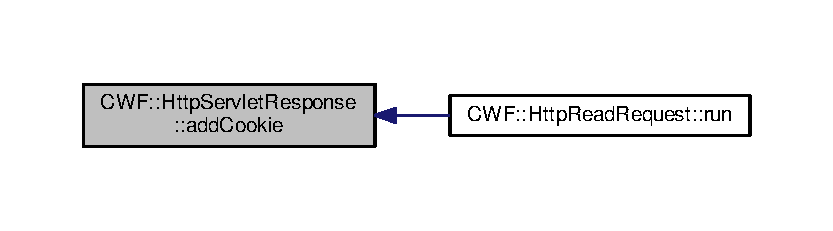
\includegraphics[width=350pt]{class_c_w_f_1_1_http_servlet_response_a3775b3aa5ffde85e61f6e1b8edb6820d_icgraph}
\end{center}
\end{figure}


\hypertarget{class_c_w_f_1_1_http_servlet_response_a2cf301ef97237d19401d398e36602472}{\index{C\+W\+F\+::\+Http\+Servlet\+Response@{C\+W\+F\+::\+Http\+Servlet\+Response}!add\+Header@{add\+Header}}
\index{add\+Header@{add\+Header}!C\+W\+F\+::\+Http\+Servlet\+Response@{C\+W\+F\+::\+Http\+Servlet\+Response}}
\subsubsection[{add\+Header}]{\setlength{\rightskip}{0pt plus 5cm}void C\+W\+F\+::\+Http\+Servlet\+Response\+::add\+Header (
\begin{DoxyParamCaption}
\item[{const Q\+Byte\+Array \&}]{name, }
\item[{const Q\+Byte\+Array \&}]{value}
\end{DoxyParamCaption}
)}}\label{class_c_w_f_1_1_http_servlet_response_a2cf301ef97237d19401d398e36602472}


Here is the caller graph for this function\+:
\nopagebreak
\begin{figure}[H]
\begin{center}
\leavevmode
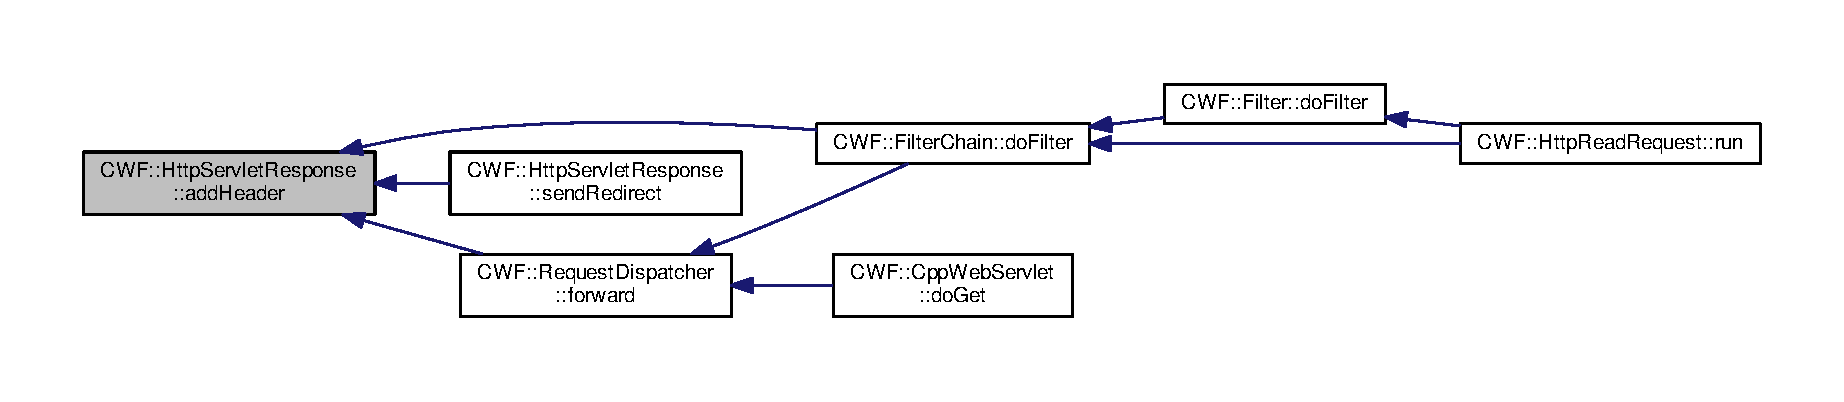
\includegraphics[width=350pt]{class_c_w_f_1_1_http_servlet_response_a2cf301ef97237d19401d398e36602472_icgraph}
\end{center}
\end{figure}


\hypertarget{class_c_w_f_1_1_http_servlet_response_acfe923500ad8cee08c5acf6767e571bc}{\index{C\+W\+F\+::\+Http\+Servlet\+Response@{C\+W\+F\+::\+Http\+Servlet\+Response}!flush\+Buffer@{flush\+Buffer}}
\index{flush\+Buffer@{flush\+Buffer}!C\+W\+F\+::\+Http\+Servlet\+Response@{C\+W\+F\+::\+Http\+Servlet\+Response}}
\subsubsection[{flush\+Buffer}]{\setlength{\rightskip}{0pt plus 5cm}void C\+W\+F\+::\+Http\+Servlet\+Response\+::flush\+Buffer (
\begin{DoxyParamCaption}
{}
\end{DoxyParamCaption}
)}}\label{class_c_w_f_1_1_http_servlet_response_acfe923500ad8cee08c5acf6767e571bc}


Here is the call graph for this function\+:
\nopagebreak
\begin{figure}[H]
\begin{center}
\leavevmode
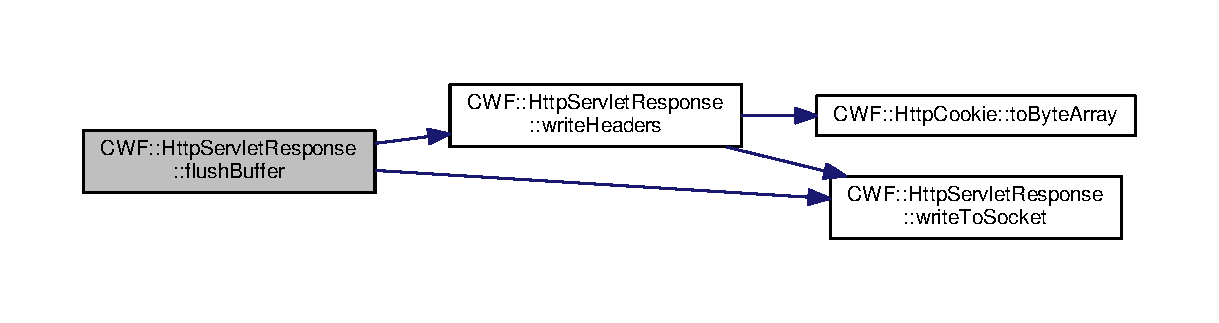
\includegraphics[width=350pt]{class_c_w_f_1_1_http_servlet_response_acfe923500ad8cee08c5acf6767e571bc_cgraph}
\end{center}
\end{figure}




Here is the caller graph for this function\+:
\nopagebreak
\begin{figure}[H]
\begin{center}
\leavevmode
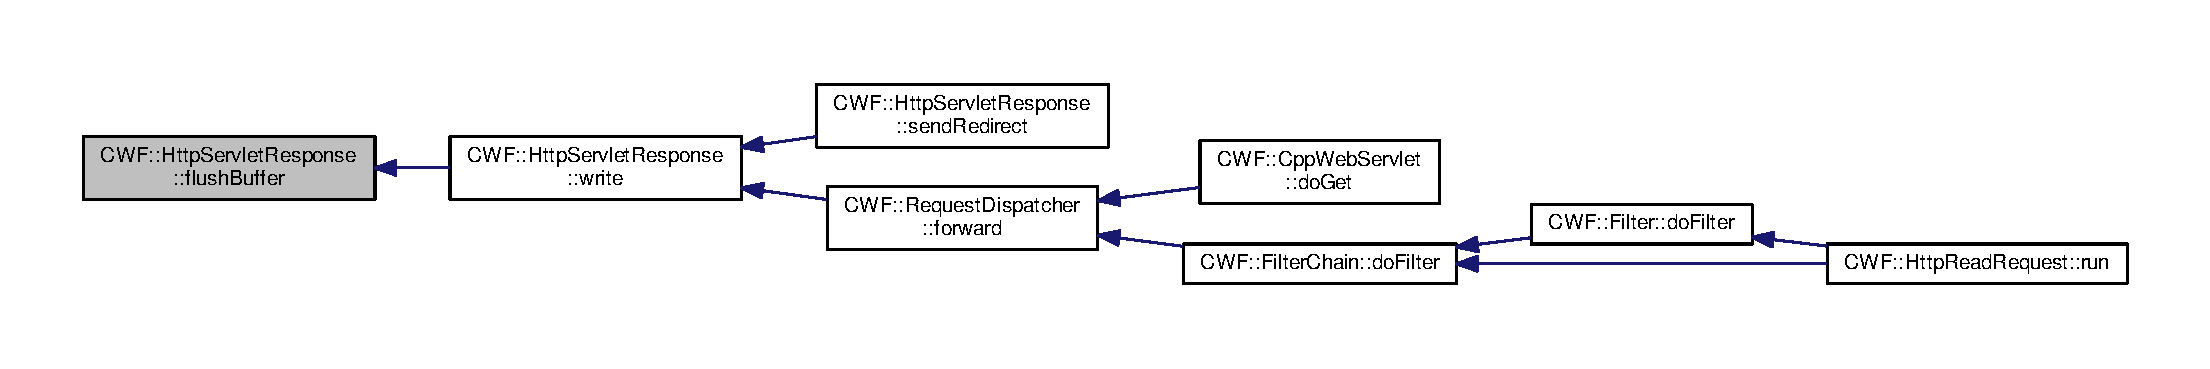
\includegraphics[width=350pt]{class_c_w_f_1_1_http_servlet_response_acfe923500ad8cee08c5acf6767e571bc_icgraph}
\end{center}
\end{figure}


\hypertarget{class_c_w_f_1_1_http_servlet_response_a11784e6485fb80078afdc00398a23ba7}{\index{C\+W\+F\+::\+Http\+Servlet\+Response@{C\+W\+F\+::\+Http\+Servlet\+Response}!get\+Buffer\+Size@{get\+Buffer\+Size}}
\index{get\+Buffer\+Size@{get\+Buffer\+Size}!C\+W\+F\+::\+Http\+Servlet\+Response@{C\+W\+F\+::\+Http\+Servlet\+Response}}
\subsubsection[{get\+Buffer\+Size}]{\setlength{\rightskip}{0pt plus 5cm}int C\+W\+F\+::\+Http\+Servlet\+Response\+::get\+Buffer\+Size (
\begin{DoxyParamCaption}
{}
\end{DoxyParamCaption}
) const}}\label{class_c_w_f_1_1_http_servlet_response_a11784e6485fb80078afdc00398a23ba7}
\hypertarget{class_c_w_f_1_1_http_servlet_response_a1b45b744de83577359fb85e1aaffc7dd}{\index{C\+W\+F\+::\+Http\+Servlet\+Response@{C\+W\+F\+::\+Http\+Servlet\+Response}!get\+Socket@{get\+Socket}}
\index{get\+Socket@{get\+Socket}!C\+W\+F\+::\+Http\+Servlet\+Response@{C\+W\+F\+::\+Http\+Servlet\+Response}}
\subsubsection[{get\+Socket}]{\setlength{\rightskip}{0pt plus 5cm}Q\+Tcp\+Socket \& C\+W\+F\+::\+Http\+Servlet\+Response\+::get\+Socket (
\begin{DoxyParamCaption}
{}
\end{DoxyParamCaption}
) const}}\label{class_c_w_f_1_1_http_servlet_response_a1b45b744de83577359fb85e1aaffc7dd}
\hypertarget{class_c_w_f_1_1_http_servlet_response_a218be925792dfe06096d63d05e28edce}{\index{C\+W\+F\+::\+Http\+Servlet\+Response@{C\+W\+F\+::\+Http\+Servlet\+Response}!send\+Error@{send\+Error}}
\index{send\+Error@{send\+Error}!C\+W\+F\+::\+Http\+Servlet\+Response@{C\+W\+F\+::\+Http\+Servlet\+Response}}
\subsubsection[{send\+Error}]{\setlength{\rightskip}{0pt plus 5cm}void C\+W\+F\+::\+Http\+Servlet\+Response\+::send\+Error (
\begin{DoxyParamCaption}
\item[{int}]{sc, }
\item[{const Q\+Byte\+Array \&}]{msg}
\end{DoxyParamCaption}
)}}\label{class_c_w_f_1_1_http_servlet_response_a218be925792dfe06096d63d05e28edce}


Here is the call graph for this function\+:
\nopagebreak
\begin{figure}[H]
\begin{center}
\leavevmode
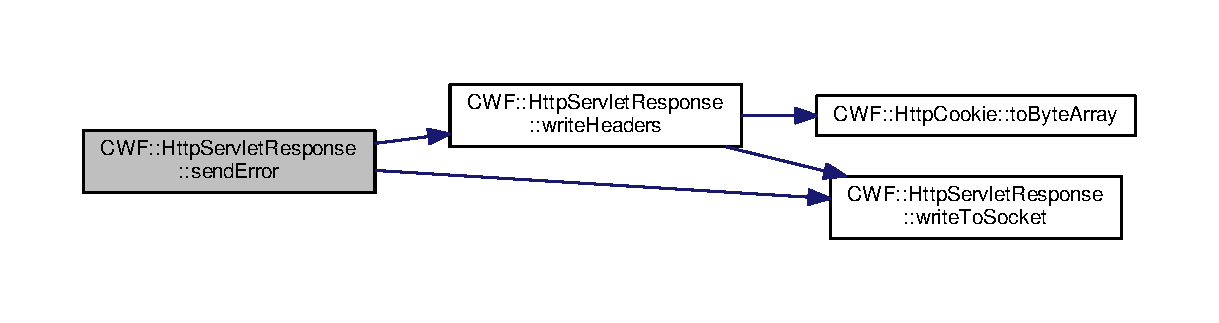
\includegraphics[width=350pt]{class_c_w_f_1_1_http_servlet_response_a218be925792dfe06096d63d05e28edce_cgraph}
\end{center}
\end{figure}


\hypertarget{class_c_w_f_1_1_http_servlet_response_a665b695119c30234b2b77665c36e010d}{\index{C\+W\+F\+::\+Http\+Servlet\+Response@{C\+W\+F\+::\+Http\+Servlet\+Response}!send\+Redirect@{send\+Redirect}}
\index{send\+Redirect@{send\+Redirect}!C\+W\+F\+::\+Http\+Servlet\+Response@{C\+W\+F\+::\+Http\+Servlet\+Response}}
\subsubsection[{send\+Redirect}]{\setlength{\rightskip}{0pt plus 5cm}void C\+W\+F\+::\+Http\+Servlet\+Response\+::send\+Redirect (
\begin{DoxyParamCaption}
\item[{const Q\+Byte\+Array \&}]{url}
\end{DoxyParamCaption}
)}}\label{class_c_w_f_1_1_http_servlet_response_a665b695119c30234b2b77665c36e010d}


Here is the call graph for this function\+:
\nopagebreak
\begin{figure}[H]
\begin{center}
\leavevmode
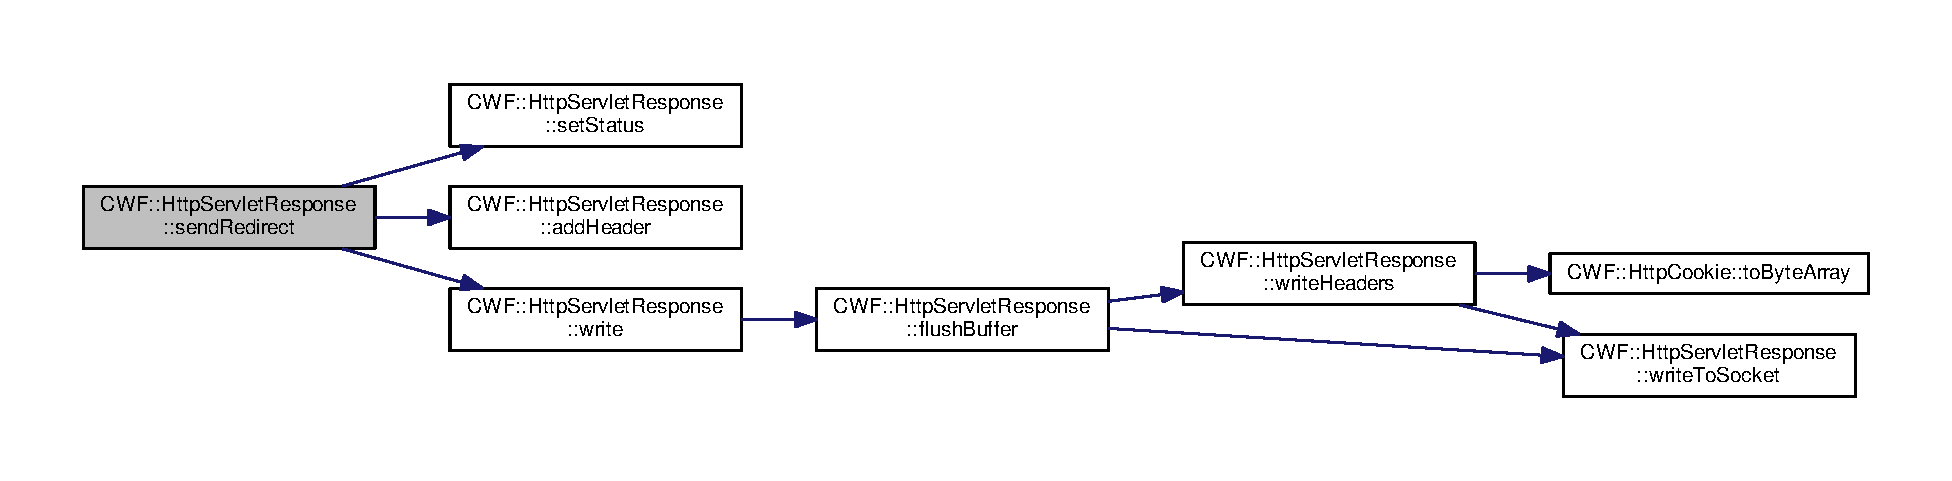
\includegraphics[width=350pt]{class_c_w_f_1_1_http_servlet_response_a665b695119c30234b2b77665c36e010d_cgraph}
\end{center}
\end{figure}


\hypertarget{class_c_w_f_1_1_http_servlet_response_aeebd12d9d9eab98fb0d1810605e8c2ab}{\index{C\+W\+F\+::\+Http\+Servlet\+Response@{C\+W\+F\+::\+Http\+Servlet\+Response}!set\+Status@{set\+Status}}
\index{set\+Status@{set\+Status}!C\+W\+F\+::\+Http\+Servlet\+Response@{C\+W\+F\+::\+Http\+Servlet\+Response}}
\subsubsection[{set\+Status}]{\setlength{\rightskip}{0pt plus 5cm}void C\+W\+F\+::\+Http\+Servlet\+Response\+::set\+Status (
\begin{DoxyParamCaption}
\item[{const int \&}]{status\+Code, }
\item[{const Q\+Byte\+Array \&}]{description}
\end{DoxyParamCaption}
)}}\label{class_c_w_f_1_1_http_servlet_response_aeebd12d9d9eab98fb0d1810605e8c2ab}


Here is the caller graph for this function\+:
\nopagebreak
\begin{figure}[H]
\begin{center}
\leavevmode
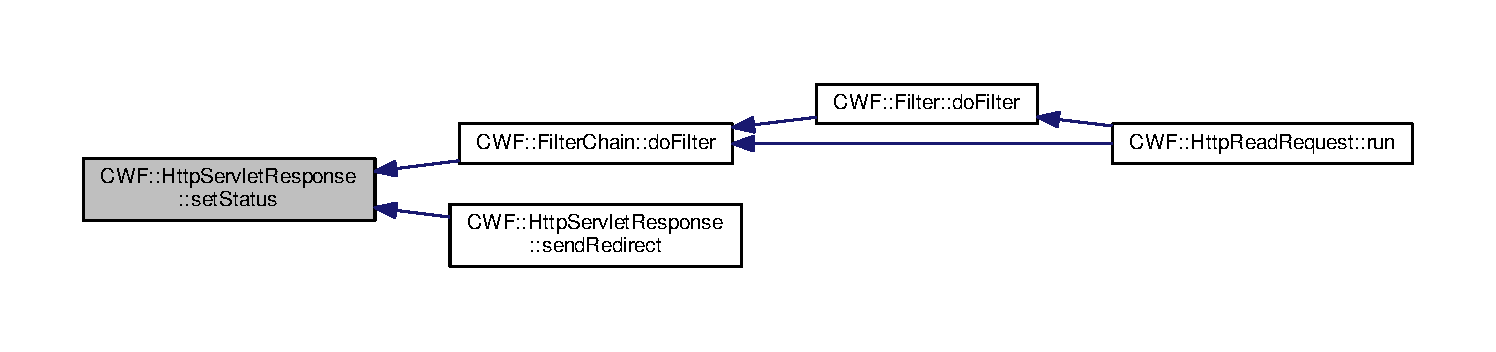
\includegraphics[width=350pt]{class_c_w_f_1_1_http_servlet_response_aeebd12d9d9eab98fb0d1810605e8c2ab_icgraph}
\end{center}
\end{figure}


\hypertarget{class_c_w_f_1_1_http_servlet_response_ae4fdbaa3d3edd4234955fadc20cb896c}{\index{C\+W\+F\+::\+Http\+Servlet\+Response@{C\+W\+F\+::\+Http\+Servlet\+Response}!write@{write}}
\index{write@{write}!C\+W\+F\+::\+Http\+Servlet\+Response@{C\+W\+F\+::\+Http\+Servlet\+Response}}
\subsubsection[{write}]{\setlength{\rightskip}{0pt plus 5cm}void C\+W\+F\+::\+Http\+Servlet\+Response\+::write (
\begin{DoxyParamCaption}
\item[{const Q\+Byte\+Array \&}]{data, }
\item[{bool}]{flush = {\ttfamily true}}
\end{DoxyParamCaption}
)}}\label{class_c_w_f_1_1_http_servlet_response_ae4fdbaa3d3edd4234955fadc20cb896c}


Here is the call graph for this function\+:
\nopagebreak
\begin{figure}[H]
\begin{center}
\leavevmode
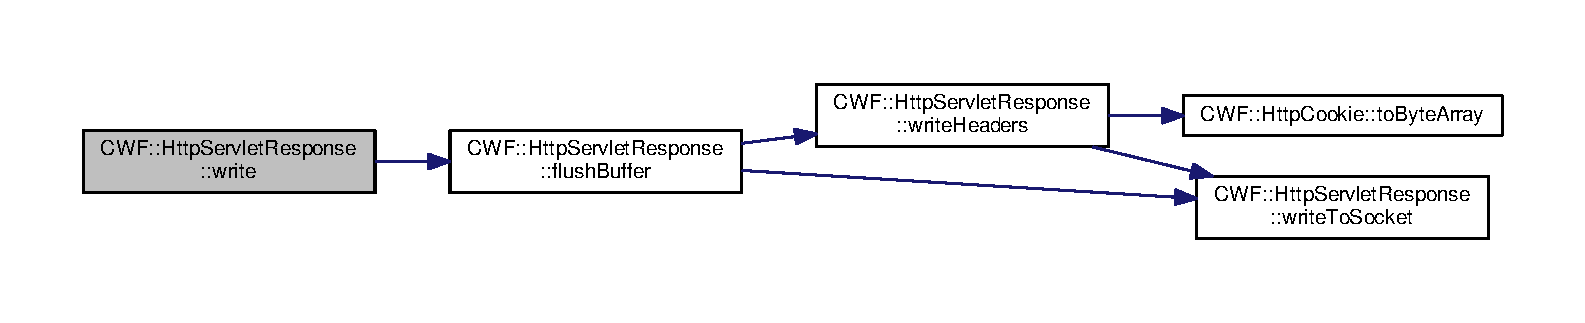
\includegraphics[width=350pt]{class_c_w_f_1_1_http_servlet_response_ae4fdbaa3d3edd4234955fadc20cb896c_cgraph}
\end{center}
\end{figure}




Here is the caller graph for this function\+:
\nopagebreak
\begin{figure}[H]
\begin{center}
\leavevmode
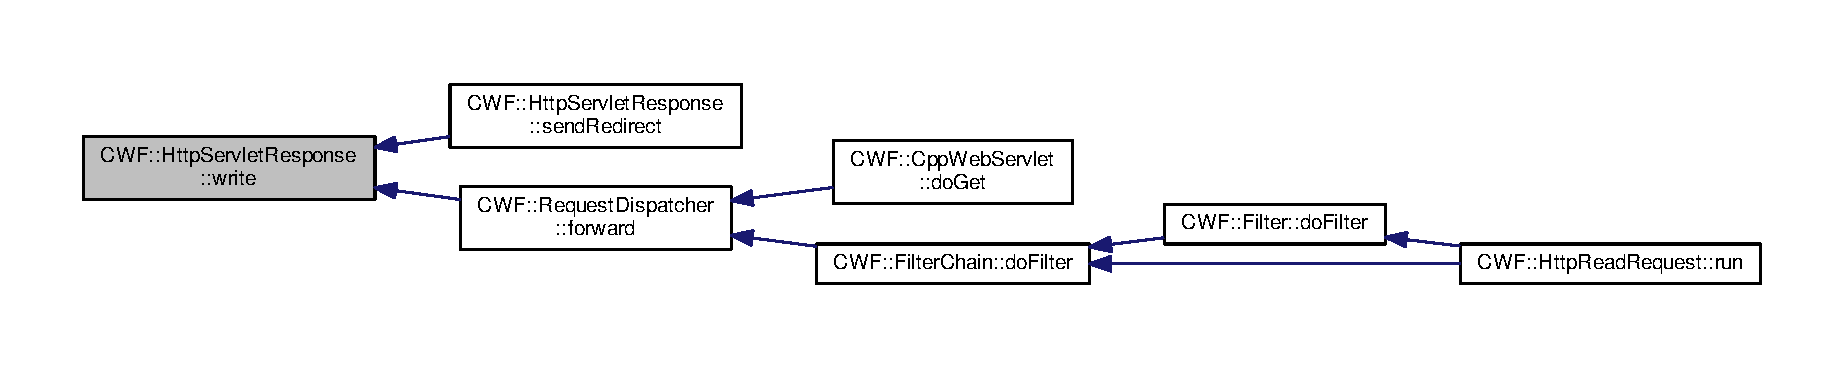
\includegraphics[width=350pt]{class_c_w_f_1_1_http_servlet_response_ae4fdbaa3d3edd4234955fadc20cb896c_icgraph}
\end{center}
\end{figure}


\hypertarget{class_c_w_f_1_1_http_servlet_response_a6a377703f21bb5578d5103acb2e397d1}{\index{C\+W\+F\+::\+Http\+Servlet\+Response@{C\+W\+F\+::\+Http\+Servlet\+Response}!write\+Headers@{write\+Headers}}
\index{write\+Headers@{write\+Headers}!C\+W\+F\+::\+Http\+Servlet\+Response@{C\+W\+F\+::\+Http\+Servlet\+Response}}
\subsubsection[{write\+Headers}]{\setlength{\rightskip}{0pt plus 5cm}void C\+W\+F\+::\+Http\+Servlet\+Response\+::write\+Headers (
\begin{DoxyParamCaption}
{}
\end{DoxyParamCaption}
)}}\label{class_c_w_f_1_1_http_servlet_response_a6a377703f21bb5578d5103acb2e397d1}


Here is the call graph for this function\+:
\nopagebreak
\begin{figure}[H]
\begin{center}
\leavevmode
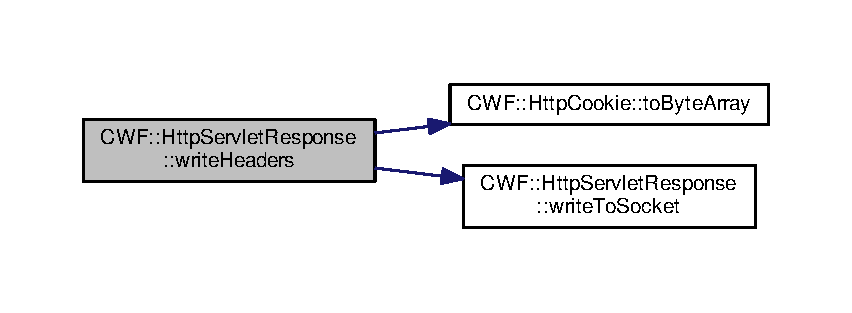
\includegraphics[width=350pt]{class_c_w_f_1_1_http_servlet_response_a6a377703f21bb5578d5103acb2e397d1_cgraph}
\end{center}
\end{figure}




Here is the caller graph for this function\+:
\nopagebreak
\begin{figure}[H]
\begin{center}
\leavevmode
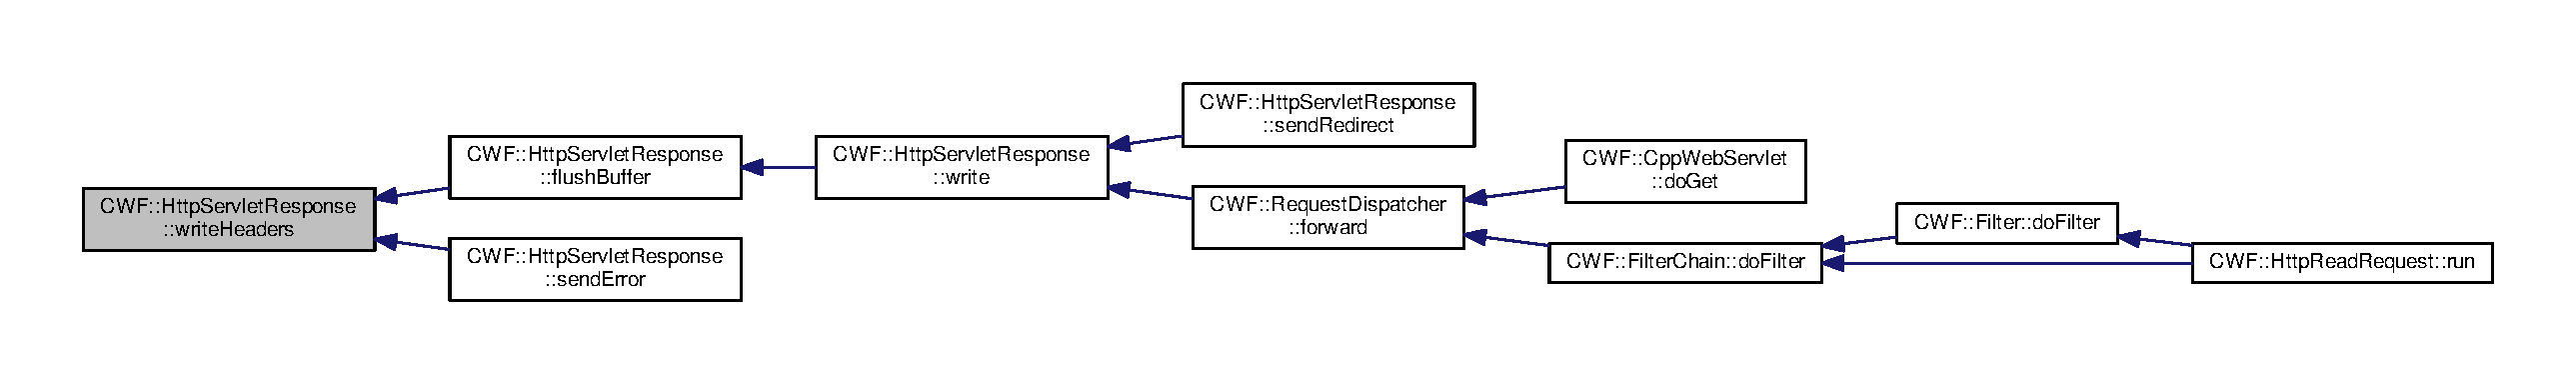
\includegraphics[width=350pt]{class_c_w_f_1_1_http_servlet_response_a6a377703f21bb5578d5103acb2e397d1_icgraph}
\end{center}
\end{figure}


\hypertarget{class_c_w_f_1_1_http_servlet_response_a1e6bf9efa60fa22dd2b058b69bd735c9}{\index{C\+W\+F\+::\+Http\+Servlet\+Response@{C\+W\+F\+::\+Http\+Servlet\+Response}!write\+To\+Socket@{write\+To\+Socket}}
\index{write\+To\+Socket@{write\+To\+Socket}!C\+W\+F\+::\+Http\+Servlet\+Response@{C\+W\+F\+::\+Http\+Servlet\+Response}}
\subsubsection[{write\+To\+Socket}]{\setlength{\rightskip}{0pt plus 5cm}void C\+W\+F\+::\+Http\+Servlet\+Response\+::write\+To\+Socket (
\begin{DoxyParamCaption}
\item[{const Q\+Byte\+Array \&}]{data}
\end{DoxyParamCaption}
)}}\label{class_c_w_f_1_1_http_servlet_response_a1e6bf9efa60fa22dd2b058b69bd735c9}


Here is the caller graph for this function\+:
\nopagebreak
\begin{figure}[H]
\begin{center}
\leavevmode
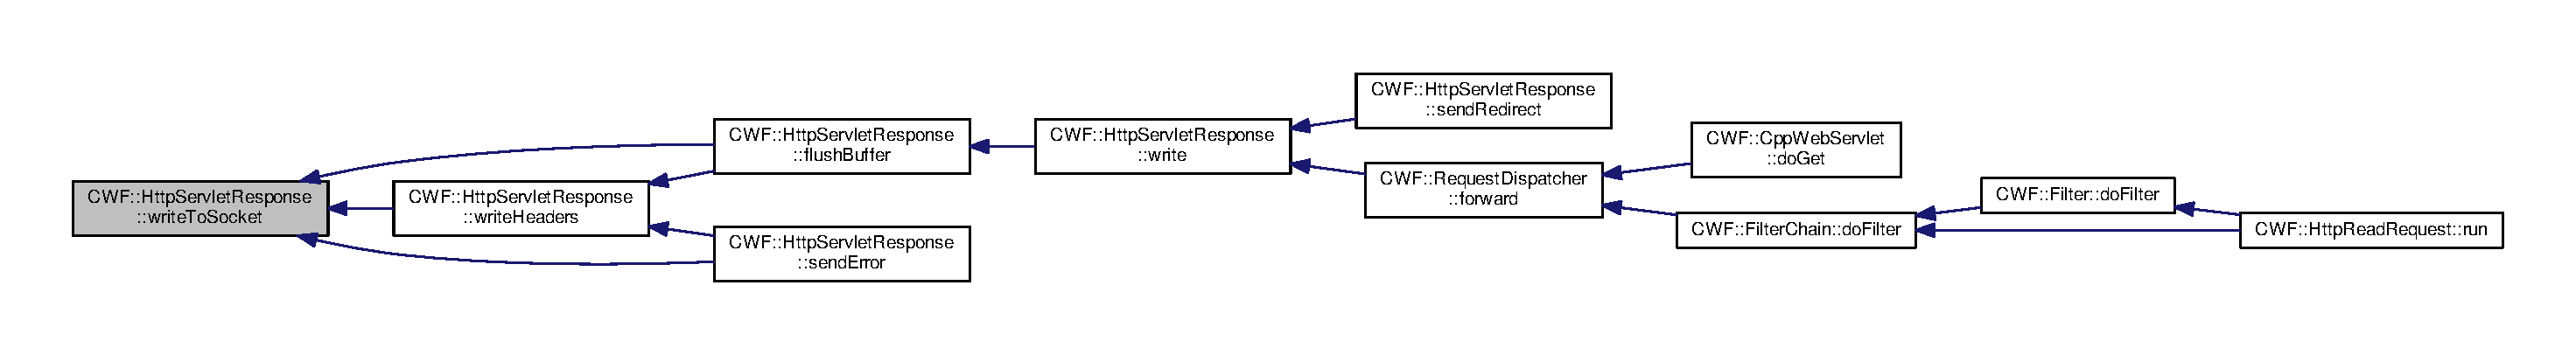
\includegraphics[width=350pt]{class_c_w_f_1_1_http_servlet_response_a1e6bf9efa60fa22dd2b058b69bd735c9_icgraph}
\end{center}
\end{figure}




\subsection{Member Data Documentation}
\hypertarget{class_c_w_f_1_1_http_servlet_response_a66c8c74a4dff06c963c4bed1339e82a8}{\index{C\+W\+F\+::\+Http\+Servlet\+Response@{C\+W\+F\+::\+Http\+Servlet\+Response}!S\+C\+\_\+\+A\+C\+C\+E\+P\+T\+E\+D@{S\+C\+\_\+\+A\+C\+C\+E\+P\+T\+E\+D}}
\index{S\+C\+\_\+\+A\+C\+C\+E\+P\+T\+E\+D@{S\+C\+\_\+\+A\+C\+C\+E\+P\+T\+E\+D}!C\+W\+F\+::\+Http\+Servlet\+Response@{C\+W\+F\+::\+Http\+Servlet\+Response}}
\subsubsection[{S\+C\+\_\+\+A\+C\+C\+E\+P\+T\+E\+D}]{\setlength{\rightskip}{0pt plus 5cm}const int C\+W\+F\+::\+Http\+Servlet\+Response\+::\+S\+C\+\_\+\+A\+C\+C\+E\+P\+T\+E\+D = 202\hspace{0.3cm}{\ttfamily [static]}}}\label{class_c_w_f_1_1_http_servlet_response_a66c8c74a4dff06c963c4bed1339e82a8}
\hypertarget{class_c_w_f_1_1_http_servlet_response_a4a3c83d68b706e422fc2c527996e55d0}{\index{C\+W\+F\+::\+Http\+Servlet\+Response@{C\+W\+F\+::\+Http\+Servlet\+Response}!S\+C\+\_\+\+B\+A\+D\+\_\+\+G\+A\+T\+E\+W\+A\+Y@{S\+C\+\_\+\+B\+A\+D\+\_\+\+G\+A\+T\+E\+W\+A\+Y}}
\index{S\+C\+\_\+\+B\+A\+D\+\_\+\+G\+A\+T\+E\+W\+A\+Y@{S\+C\+\_\+\+B\+A\+D\+\_\+\+G\+A\+T\+E\+W\+A\+Y}!C\+W\+F\+::\+Http\+Servlet\+Response@{C\+W\+F\+::\+Http\+Servlet\+Response}}
\subsubsection[{S\+C\+\_\+\+B\+A\+D\+\_\+\+G\+A\+T\+E\+W\+A\+Y}]{\setlength{\rightskip}{0pt plus 5cm}const int C\+W\+F\+::\+Http\+Servlet\+Response\+::\+S\+C\+\_\+\+B\+A\+D\+\_\+\+G\+A\+T\+E\+W\+A\+Y = 502\hspace{0.3cm}{\ttfamily [static]}}}\label{class_c_w_f_1_1_http_servlet_response_a4a3c83d68b706e422fc2c527996e55d0}
\hypertarget{class_c_w_f_1_1_http_servlet_response_ac85b62a3e41626ed44cec21e68c70839}{\index{C\+W\+F\+::\+Http\+Servlet\+Response@{C\+W\+F\+::\+Http\+Servlet\+Response}!S\+C\+\_\+\+B\+A\+D\+\_\+\+R\+E\+Q\+U\+E\+S\+T@{S\+C\+\_\+\+B\+A\+D\+\_\+\+R\+E\+Q\+U\+E\+S\+T}}
\index{S\+C\+\_\+\+B\+A\+D\+\_\+\+R\+E\+Q\+U\+E\+S\+T@{S\+C\+\_\+\+B\+A\+D\+\_\+\+R\+E\+Q\+U\+E\+S\+T}!C\+W\+F\+::\+Http\+Servlet\+Response@{C\+W\+F\+::\+Http\+Servlet\+Response}}
\subsubsection[{S\+C\+\_\+\+B\+A\+D\+\_\+\+R\+E\+Q\+U\+E\+S\+T}]{\setlength{\rightskip}{0pt plus 5cm}const int C\+W\+F\+::\+Http\+Servlet\+Response\+::\+S\+C\+\_\+\+B\+A\+D\+\_\+\+R\+E\+Q\+U\+E\+S\+T = 400\hspace{0.3cm}{\ttfamily [static]}}}\label{class_c_w_f_1_1_http_servlet_response_ac85b62a3e41626ed44cec21e68c70839}
\hypertarget{class_c_w_f_1_1_http_servlet_response_aff39227c80ce7554ffc4d14744566936}{\index{C\+W\+F\+::\+Http\+Servlet\+Response@{C\+W\+F\+::\+Http\+Servlet\+Response}!S\+C\+\_\+\+C\+O\+N\+F\+L\+I\+C\+T@{S\+C\+\_\+\+C\+O\+N\+F\+L\+I\+C\+T}}
\index{S\+C\+\_\+\+C\+O\+N\+F\+L\+I\+C\+T@{S\+C\+\_\+\+C\+O\+N\+F\+L\+I\+C\+T}!C\+W\+F\+::\+Http\+Servlet\+Response@{C\+W\+F\+::\+Http\+Servlet\+Response}}
\subsubsection[{S\+C\+\_\+\+C\+O\+N\+F\+L\+I\+C\+T}]{\setlength{\rightskip}{0pt plus 5cm}const int C\+W\+F\+::\+Http\+Servlet\+Response\+::\+S\+C\+\_\+\+C\+O\+N\+F\+L\+I\+C\+T = 409\hspace{0.3cm}{\ttfamily [static]}}}\label{class_c_w_f_1_1_http_servlet_response_aff39227c80ce7554ffc4d14744566936}
\hypertarget{class_c_w_f_1_1_http_servlet_response_a9eed2d26367e45b99468d96a00a75d79}{\index{C\+W\+F\+::\+Http\+Servlet\+Response@{C\+W\+F\+::\+Http\+Servlet\+Response}!S\+C\+\_\+\+C\+O\+N\+T\+I\+N\+U\+E@{S\+C\+\_\+\+C\+O\+N\+T\+I\+N\+U\+E}}
\index{S\+C\+\_\+\+C\+O\+N\+T\+I\+N\+U\+E@{S\+C\+\_\+\+C\+O\+N\+T\+I\+N\+U\+E}!C\+W\+F\+::\+Http\+Servlet\+Response@{C\+W\+F\+::\+Http\+Servlet\+Response}}
\subsubsection[{S\+C\+\_\+\+C\+O\+N\+T\+I\+N\+U\+E}]{\setlength{\rightskip}{0pt plus 5cm}const int C\+W\+F\+::\+Http\+Servlet\+Response\+::\+S\+C\+\_\+\+C\+O\+N\+T\+I\+N\+U\+E = 100\hspace{0.3cm}{\ttfamily [static]}}}\label{class_c_w_f_1_1_http_servlet_response_a9eed2d26367e45b99468d96a00a75d79}
\hypertarget{class_c_w_f_1_1_http_servlet_response_aeb04e62ba36dc6c19270202ebd636402}{\index{C\+W\+F\+::\+Http\+Servlet\+Response@{C\+W\+F\+::\+Http\+Servlet\+Response}!S\+C\+\_\+\+C\+R\+E\+A\+T\+E\+D@{S\+C\+\_\+\+C\+R\+E\+A\+T\+E\+D}}
\index{S\+C\+\_\+\+C\+R\+E\+A\+T\+E\+D@{S\+C\+\_\+\+C\+R\+E\+A\+T\+E\+D}!C\+W\+F\+::\+Http\+Servlet\+Response@{C\+W\+F\+::\+Http\+Servlet\+Response}}
\subsubsection[{S\+C\+\_\+\+C\+R\+E\+A\+T\+E\+D}]{\setlength{\rightskip}{0pt plus 5cm}const int C\+W\+F\+::\+Http\+Servlet\+Response\+::\+S\+C\+\_\+\+C\+R\+E\+A\+T\+E\+D = 201\hspace{0.3cm}{\ttfamily [static]}}}\label{class_c_w_f_1_1_http_servlet_response_aeb04e62ba36dc6c19270202ebd636402}
\hypertarget{class_c_w_f_1_1_http_servlet_response_a6c788faebc283d58933d369d28541b4f}{\index{C\+W\+F\+::\+Http\+Servlet\+Response@{C\+W\+F\+::\+Http\+Servlet\+Response}!S\+C\+\_\+\+E\+X\+P\+E\+C\+T\+A\+T\+I\+O\+N\+\_\+\+F\+A\+I\+L\+E\+D@{S\+C\+\_\+\+E\+X\+P\+E\+C\+T\+A\+T\+I\+O\+N\+\_\+\+F\+A\+I\+L\+E\+D}}
\index{S\+C\+\_\+\+E\+X\+P\+E\+C\+T\+A\+T\+I\+O\+N\+\_\+\+F\+A\+I\+L\+E\+D@{S\+C\+\_\+\+E\+X\+P\+E\+C\+T\+A\+T\+I\+O\+N\+\_\+\+F\+A\+I\+L\+E\+D}!C\+W\+F\+::\+Http\+Servlet\+Response@{C\+W\+F\+::\+Http\+Servlet\+Response}}
\subsubsection[{S\+C\+\_\+\+E\+X\+P\+E\+C\+T\+A\+T\+I\+O\+N\+\_\+\+F\+A\+I\+L\+E\+D}]{\setlength{\rightskip}{0pt plus 5cm}const int C\+W\+F\+::\+Http\+Servlet\+Response\+::\+S\+C\+\_\+\+E\+X\+P\+E\+C\+T\+A\+T\+I\+O\+N\+\_\+\+F\+A\+I\+L\+E\+D = 417\hspace{0.3cm}{\ttfamily [static]}}}\label{class_c_w_f_1_1_http_servlet_response_a6c788faebc283d58933d369d28541b4f}
\hypertarget{class_c_w_f_1_1_http_servlet_response_a899c9e06fb7475efbceccde31bc4b84c}{\index{C\+W\+F\+::\+Http\+Servlet\+Response@{C\+W\+F\+::\+Http\+Servlet\+Response}!S\+C\+\_\+\+F\+O\+R\+B\+I\+D\+D\+E\+N@{S\+C\+\_\+\+F\+O\+R\+B\+I\+D\+D\+E\+N}}
\index{S\+C\+\_\+\+F\+O\+R\+B\+I\+D\+D\+E\+N@{S\+C\+\_\+\+F\+O\+R\+B\+I\+D\+D\+E\+N}!C\+W\+F\+::\+Http\+Servlet\+Response@{C\+W\+F\+::\+Http\+Servlet\+Response}}
\subsubsection[{S\+C\+\_\+\+F\+O\+R\+B\+I\+D\+D\+E\+N}]{\setlength{\rightskip}{0pt plus 5cm}const int C\+W\+F\+::\+Http\+Servlet\+Response\+::\+S\+C\+\_\+\+F\+O\+R\+B\+I\+D\+D\+E\+N = 403\hspace{0.3cm}{\ttfamily [static]}}}\label{class_c_w_f_1_1_http_servlet_response_a899c9e06fb7475efbceccde31bc4b84c}
\hypertarget{class_c_w_f_1_1_http_servlet_response_a02d7f3f3f97fbad5efff90f7bcdbb13f}{\index{C\+W\+F\+::\+Http\+Servlet\+Response@{C\+W\+F\+::\+Http\+Servlet\+Response}!S\+C\+\_\+\+F\+O\+U\+N\+D@{S\+C\+\_\+\+F\+O\+U\+N\+D}}
\index{S\+C\+\_\+\+F\+O\+U\+N\+D@{S\+C\+\_\+\+F\+O\+U\+N\+D}!C\+W\+F\+::\+Http\+Servlet\+Response@{C\+W\+F\+::\+Http\+Servlet\+Response}}
\subsubsection[{S\+C\+\_\+\+F\+O\+U\+N\+D}]{\setlength{\rightskip}{0pt plus 5cm}const int C\+W\+F\+::\+Http\+Servlet\+Response\+::\+S\+C\+\_\+\+F\+O\+U\+N\+D = 302\hspace{0.3cm}{\ttfamily [static]}}}\label{class_c_w_f_1_1_http_servlet_response_a02d7f3f3f97fbad5efff90f7bcdbb13f}
\hypertarget{class_c_w_f_1_1_http_servlet_response_ab4dbd5c923e4a66dbbc7a3f5801fd1a9}{\index{C\+W\+F\+::\+Http\+Servlet\+Response@{C\+W\+F\+::\+Http\+Servlet\+Response}!S\+C\+\_\+\+G\+A\+T\+E\+W\+A\+Y\+\_\+\+T\+I\+M\+E\+O\+U\+T@{S\+C\+\_\+\+G\+A\+T\+E\+W\+A\+Y\+\_\+\+T\+I\+M\+E\+O\+U\+T}}
\index{S\+C\+\_\+\+G\+A\+T\+E\+W\+A\+Y\+\_\+\+T\+I\+M\+E\+O\+U\+T@{S\+C\+\_\+\+G\+A\+T\+E\+W\+A\+Y\+\_\+\+T\+I\+M\+E\+O\+U\+T}!C\+W\+F\+::\+Http\+Servlet\+Response@{C\+W\+F\+::\+Http\+Servlet\+Response}}
\subsubsection[{S\+C\+\_\+\+G\+A\+T\+E\+W\+A\+Y\+\_\+\+T\+I\+M\+E\+O\+U\+T}]{\setlength{\rightskip}{0pt plus 5cm}const int C\+W\+F\+::\+Http\+Servlet\+Response\+::\+S\+C\+\_\+\+G\+A\+T\+E\+W\+A\+Y\+\_\+\+T\+I\+M\+E\+O\+U\+T = 504\hspace{0.3cm}{\ttfamily [static]}}}\label{class_c_w_f_1_1_http_servlet_response_ab4dbd5c923e4a66dbbc7a3f5801fd1a9}
\hypertarget{class_c_w_f_1_1_http_servlet_response_ac946b14d07ec4dd5424dda38cc880583}{\index{C\+W\+F\+::\+Http\+Servlet\+Response@{C\+W\+F\+::\+Http\+Servlet\+Response}!S\+C\+\_\+\+G\+O\+N\+E@{S\+C\+\_\+\+G\+O\+N\+E}}
\index{S\+C\+\_\+\+G\+O\+N\+E@{S\+C\+\_\+\+G\+O\+N\+E}!C\+W\+F\+::\+Http\+Servlet\+Response@{C\+W\+F\+::\+Http\+Servlet\+Response}}
\subsubsection[{S\+C\+\_\+\+G\+O\+N\+E}]{\setlength{\rightskip}{0pt plus 5cm}const int C\+W\+F\+::\+Http\+Servlet\+Response\+::\+S\+C\+\_\+\+G\+O\+N\+E = 410\hspace{0.3cm}{\ttfamily [static]}}}\label{class_c_w_f_1_1_http_servlet_response_ac946b14d07ec4dd5424dda38cc880583}
\hypertarget{class_c_w_f_1_1_http_servlet_response_a105b64e573a5c1cf04f6552225bddf54}{\index{C\+W\+F\+::\+Http\+Servlet\+Response@{C\+W\+F\+::\+Http\+Servlet\+Response}!S\+C\+\_\+\+H\+T\+T\+P\+\_\+\+V\+E\+R\+S\+I\+O\+N\+\_\+\+N\+O\+T\+\_\+\+S\+U\+P\+P\+O\+R\+T\+E\+D@{S\+C\+\_\+\+H\+T\+T\+P\+\_\+\+V\+E\+R\+S\+I\+O\+N\+\_\+\+N\+O\+T\+\_\+\+S\+U\+P\+P\+O\+R\+T\+E\+D}}
\index{S\+C\+\_\+\+H\+T\+T\+P\+\_\+\+V\+E\+R\+S\+I\+O\+N\+\_\+\+N\+O\+T\+\_\+\+S\+U\+P\+P\+O\+R\+T\+E\+D@{S\+C\+\_\+\+H\+T\+T\+P\+\_\+\+V\+E\+R\+S\+I\+O\+N\+\_\+\+N\+O\+T\+\_\+\+S\+U\+P\+P\+O\+R\+T\+E\+D}!C\+W\+F\+::\+Http\+Servlet\+Response@{C\+W\+F\+::\+Http\+Servlet\+Response}}
\subsubsection[{S\+C\+\_\+\+H\+T\+T\+P\+\_\+\+V\+E\+R\+S\+I\+O\+N\+\_\+\+N\+O\+T\+\_\+\+S\+U\+P\+P\+O\+R\+T\+E\+D}]{\setlength{\rightskip}{0pt plus 5cm}const int C\+W\+F\+::\+Http\+Servlet\+Response\+::\+S\+C\+\_\+\+H\+T\+T\+P\+\_\+\+V\+E\+R\+S\+I\+O\+N\+\_\+\+N\+O\+T\+\_\+\+S\+U\+P\+P\+O\+R\+T\+E\+D = 505\hspace{0.3cm}{\ttfamily [static]}}}\label{class_c_w_f_1_1_http_servlet_response_a105b64e573a5c1cf04f6552225bddf54}
\hypertarget{class_c_w_f_1_1_http_servlet_response_aa405174745632134d866115233de2371}{\index{C\+W\+F\+::\+Http\+Servlet\+Response@{C\+W\+F\+::\+Http\+Servlet\+Response}!S\+C\+\_\+\+I\+N\+T\+E\+R\+N\+A\+L\+\_\+\+S\+E\+R\+V\+E\+R\+\_\+\+E\+R\+R\+O\+R@{S\+C\+\_\+\+I\+N\+T\+E\+R\+N\+A\+L\+\_\+\+S\+E\+R\+V\+E\+R\+\_\+\+E\+R\+R\+O\+R}}
\index{S\+C\+\_\+\+I\+N\+T\+E\+R\+N\+A\+L\+\_\+\+S\+E\+R\+V\+E\+R\+\_\+\+E\+R\+R\+O\+R@{S\+C\+\_\+\+I\+N\+T\+E\+R\+N\+A\+L\+\_\+\+S\+E\+R\+V\+E\+R\+\_\+\+E\+R\+R\+O\+R}!C\+W\+F\+::\+Http\+Servlet\+Response@{C\+W\+F\+::\+Http\+Servlet\+Response}}
\subsubsection[{S\+C\+\_\+\+I\+N\+T\+E\+R\+N\+A\+L\+\_\+\+S\+E\+R\+V\+E\+R\+\_\+\+E\+R\+R\+O\+R}]{\setlength{\rightskip}{0pt plus 5cm}const int C\+W\+F\+::\+Http\+Servlet\+Response\+::\+S\+C\+\_\+\+I\+N\+T\+E\+R\+N\+A\+L\+\_\+\+S\+E\+R\+V\+E\+R\+\_\+\+E\+R\+R\+O\+R = 500\hspace{0.3cm}{\ttfamily [static]}}}\label{class_c_w_f_1_1_http_servlet_response_aa405174745632134d866115233de2371}
\hypertarget{class_c_w_f_1_1_http_servlet_response_a5cc3ca43e4d370b061e7ce6e97482dad}{\index{C\+W\+F\+::\+Http\+Servlet\+Response@{C\+W\+F\+::\+Http\+Servlet\+Response}!S\+C\+\_\+\+L\+E\+N\+G\+T\+H\+\_\+\+R\+E\+Q\+U\+I\+R\+E\+D@{S\+C\+\_\+\+L\+E\+N\+G\+T\+H\+\_\+\+R\+E\+Q\+U\+I\+R\+E\+D}}
\index{S\+C\+\_\+\+L\+E\+N\+G\+T\+H\+\_\+\+R\+E\+Q\+U\+I\+R\+E\+D@{S\+C\+\_\+\+L\+E\+N\+G\+T\+H\+\_\+\+R\+E\+Q\+U\+I\+R\+E\+D}!C\+W\+F\+::\+Http\+Servlet\+Response@{C\+W\+F\+::\+Http\+Servlet\+Response}}
\subsubsection[{S\+C\+\_\+\+L\+E\+N\+G\+T\+H\+\_\+\+R\+E\+Q\+U\+I\+R\+E\+D}]{\setlength{\rightskip}{0pt plus 5cm}const int C\+W\+F\+::\+Http\+Servlet\+Response\+::\+S\+C\+\_\+\+L\+E\+N\+G\+T\+H\+\_\+\+R\+E\+Q\+U\+I\+R\+E\+D = 411\hspace{0.3cm}{\ttfamily [static]}}}\label{class_c_w_f_1_1_http_servlet_response_a5cc3ca43e4d370b061e7ce6e97482dad}
\hypertarget{class_c_w_f_1_1_http_servlet_response_a256fa073bac8902a5339d87d5e201a6e}{\index{C\+W\+F\+::\+Http\+Servlet\+Response@{C\+W\+F\+::\+Http\+Servlet\+Response}!S\+C\+\_\+\+M\+E\+T\+H\+O\+D\+\_\+\+N\+O\+T\+\_\+\+A\+L\+L\+O\+W\+E\+D@{S\+C\+\_\+\+M\+E\+T\+H\+O\+D\+\_\+\+N\+O\+T\+\_\+\+A\+L\+L\+O\+W\+E\+D}}
\index{S\+C\+\_\+\+M\+E\+T\+H\+O\+D\+\_\+\+N\+O\+T\+\_\+\+A\+L\+L\+O\+W\+E\+D@{S\+C\+\_\+\+M\+E\+T\+H\+O\+D\+\_\+\+N\+O\+T\+\_\+\+A\+L\+L\+O\+W\+E\+D}!C\+W\+F\+::\+Http\+Servlet\+Response@{C\+W\+F\+::\+Http\+Servlet\+Response}}
\subsubsection[{S\+C\+\_\+\+M\+E\+T\+H\+O\+D\+\_\+\+N\+O\+T\+\_\+\+A\+L\+L\+O\+W\+E\+D}]{\setlength{\rightskip}{0pt plus 5cm}const int C\+W\+F\+::\+Http\+Servlet\+Response\+::\+S\+C\+\_\+\+M\+E\+T\+H\+O\+D\+\_\+\+N\+O\+T\+\_\+\+A\+L\+L\+O\+W\+E\+D = 405\hspace{0.3cm}{\ttfamily [static]}}}\label{class_c_w_f_1_1_http_servlet_response_a256fa073bac8902a5339d87d5e201a6e}
\hypertarget{class_c_w_f_1_1_http_servlet_response_a1d3b0d0bcdea47e2cbcf872d4a3fbac6}{\index{C\+W\+F\+::\+Http\+Servlet\+Response@{C\+W\+F\+::\+Http\+Servlet\+Response}!S\+C\+\_\+\+M\+O\+V\+E\+D\+\_\+\+P\+E\+R\+M\+A\+N\+E\+N\+T\+L\+Y@{S\+C\+\_\+\+M\+O\+V\+E\+D\+\_\+\+P\+E\+R\+M\+A\+N\+E\+N\+T\+L\+Y}}
\index{S\+C\+\_\+\+M\+O\+V\+E\+D\+\_\+\+P\+E\+R\+M\+A\+N\+E\+N\+T\+L\+Y@{S\+C\+\_\+\+M\+O\+V\+E\+D\+\_\+\+P\+E\+R\+M\+A\+N\+E\+N\+T\+L\+Y}!C\+W\+F\+::\+Http\+Servlet\+Response@{C\+W\+F\+::\+Http\+Servlet\+Response}}
\subsubsection[{S\+C\+\_\+\+M\+O\+V\+E\+D\+\_\+\+P\+E\+R\+M\+A\+N\+E\+N\+T\+L\+Y}]{\setlength{\rightskip}{0pt plus 5cm}const int C\+W\+F\+::\+Http\+Servlet\+Response\+::\+S\+C\+\_\+\+M\+O\+V\+E\+D\+\_\+\+P\+E\+R\+M\+A\+N\+E\+N\+T\+L\+Y = 301\hspace{0.3cm}{\ttfamily [static]}}}\label{class_c_w_f_1_1_http_servlet_response_a1d3b0d0bcdea47e2cbcf872d4a3fbac6}
\hypertarget{class_c_w_f_1_1_http_servlet_response_a9561af26ae9b74f8d9dda5d234df77d3}{\index{C\+W\+F\+::\+Http\+Servlet\+Response@{C\+W\+F\+::\+Http\+Servlet\+Response}!S\+C\+\_\+\+M\+O\+V\+E\+D\+\_\+\+T\+E\+M\+P\+O\+R\+A\+R\+I\+L\+Y@{S\+C\+\_\+\+M\+O\+V\+E\+D\+\_\+\+T\+E\+M\+P\+O\+R\+A\+R\+I\+L\+Y}}
\index{S\+C\+\_\+\+M\+O\+V\+E\+D\+\_\+\+T\+E\+M\+P\+O\+R\+A\+R\+I\+L\+Y@{S\+C\+\_\+\+M\+O\+V\+E\+D\+\_\+\+T\+E\+M\+P\+O\+R\+A\+R\+I\+L\+Y}!C\+W\+F\+::\+Http\+Servlet\+Response@{C\+W\+F\+::\+Http\+Servlet\+Response}}
\subsubsection[{S\+C\+\_\+\+M\+O\+V\+E\+D\+\_\+\+T\+E\+M\+P\+O\+R\+A\+R\+I\+L\+Y}]{\setlength{\rightskip}{0pt plus 5cm}const int C\+W\+F\+::\+Http\+Servlet\+Response\+::\+S\+C\+\_\+\+M\+O\+V\+E\+D\+\_\+\+T\+E\+M\+P\+O\+R\+A\+R\+I\+L\+Y = 302\hspace{0.3cm}{\ttfamily [static]}}}\label{class_c_w_f_1_1_http_servlet_response_a9561af26ae9b74f8d9dda5d234df77d3}
\hypertarget{class_c_w_f_1_1_http_servlet_response_a9d329691713f290b9fb86a12680edc57}{\index{C\+W\+F\+::\+Http\+Servlet\+Response@{C\+W\+F\+::\+Http\+Servlet\+Response}!S\+C\+\_\+\+M\+U\+L\+T\+I\+P\+L\+E\+\_\+\+C\+H\+O\+I\+C\+E\+S@{S\+C\+\_\+\+M\+U\+L\+T\+I\+P\+L\+E\+\_\+\+C\+H\+O\+I\+C\+E\+S}}
\index{S\+C\+\_\+\+M\+U\+L\+T\+I\+P\+L\+E\+\_\+\+C\+H\+O\+I\+C\+E\+S@{S\+C\+\_\+\+M\+U\+L\+T\+I\+P\+L\+E\+\_\+\+C\+H\+O\+I\+C\+E\+S}!C\+W\+F\+::\+Http\+Servlet\+Response@{C\+W\+F\+::\+Http\+Servlet\+Response}}
\subsubsection[{S\+C\+\_\+\+M\+U\+L\+T\+I\+P\+L\+E\+\_\+\+C\+H\+O\+I\+C\+E\+S}]{\setlength{\rightskip}{0pt plus 5cm}const int C\+W\+F\+::\+Http\+Servlet\+Response\+::\+S\+C\+\_\+\+M\+U\+L\+T\+I\+P\+L\+E\+\_\+\+C\+H\+O\+I\+C\+E\+S = 300\hspace{0.3cm}{\ttfamily [static]}}}\label{class_c_w_f_1_1_http_servlet_response_a9d329691713f290b9fb86a12680edc57}
\hypertarget{class_c_w_f_1_1_http_servlet_response_afe498f5d02ddf5fb32962658ed3e8e8d}{\index{C\+W\+F\+::\+Http\+Servlet\+Response@{C\+W\+F\+::\+Http\+Servlet\+Response}!S\+C\+\_\+\+N\+O\+\_\+\+C\+O\+N\+T\+E\+N\+T@{S\+C\+\_\+\+N\+O\+\_\+\+C\+O\+N\+T\+E\+N\+T}}
\index{S\+C\+\_\+\+N\+O\+\_\+\+C\+O\+N\+T\+E\+N\+T@{S\+C\+\_\+\+N\+O\+\_\+\+C\+O\+N\+T\+E\+N\+T}!C\+W\+F\+::\+Http\+Servlet\+Response@{C\+W\+F\+::\+Http\+Servlet\+Response}}
\subsubsection[{S\+C\+\_\+\+N\+O\+\_\+\+C\+O\+N\+T\+E\+N\+T}]{\setlength{\rightskip}{0pt plus 5cm}const int C\+W\+F\+::\+Http\+Servlet\+Response\+::\+S\+C\+\_\+\+N\+O\+\_\+\+C\+O\+N\+T\+E\+N\+T = 204\hspace{0.3cm}{\ttfamily [static]}}}\label{class_c_w_f_1_1_http_servlet_response_afe498f5d02ddf5fb32962658ed3e8e8d}
\hypertarget{class_c_w_f_1_1_http_servlet_response_a5b617684845489bee4b7c3b73c1aebeb}{\index{C\+W\+F\+::\+Http\+Servlet\+Response@{C\+W\+F\+::\+Http\+Servlet\+Response}!S\+C\+\_\+\+N\+O\+N\+\_\+\+A\+U\+T\+H\+O\+R\+I\+T\+A\+T\+I\+V\+E\+\_\+\+I\+N\+F\+O\+R\+M\+A\+T\+I\+O\+N@{S\+C\+\_\+\+N\+O\+N\+\_\+\+A\+U\+T\+H\+O\+R\+I\+T\+A\+T\+I\+V\+E\+\_\+\+I\+N\+F\+O\+R\+M\+A\+T\+I\+O\+N}}
\index{S\+C\+\_\+\+N\+O\+N\+\_\+\+A\+U\+T\+H\+O\+R\+I\+T\+A\+T\+I\+V\+E\+\_\+\+I\+N\+F\+O\+R\+M\+A\+T\+I\+O\+N@{S\+C\+\_\+\+N\+O\+N\+\_\+\+A\+U\+T\+H\+O\+R\+I\+T\+A\+T\+I\+V\+E\+\_\+\+I\+N\+F\+O\+R\+M\+A\+T\+I\+O\+N}!C\+W\+F\+::\+Http\+Servlet\+Response@{C\+W\+F\+::\+Http\+Servlet\+Response}}
\subsubsection[{S\+C\+\_\+\+N\+O\+N\+\_\+\+A\+U\+T\+H\+O\+R\+I\+T\+A\+T\+I\+V\+E\+\_\+\+I\+N\+F\+O\+R\+M\+A\+T\+I\+O\+N}]{\setlength{\rightskip}{0pt plus 5cm}const int C\+W\+F\+::\+Http\+Servlet\+Response\+::\+S\+C\+\_\+\+N\+O\+N\+\_\+\+A\+U\+T\+H\+O\+R\+I\+T\+A\+T\+I\+V\+E\+\_\+\+I\+N\+F\+O\+R\+M\+A\+T\+I\+O\+N = 203\hspace{0.3cm}{\ttfamily [static]}}}\label{class_c_w_f_1_1_http_servlet_response_a5b617684845489bee4b7c3b73c1aebeb}
\hypertarget{class_c_w_f_1_1_http_servlet_response_a6bee649100ca47b85e3514739299a41a}{\index{C\+W\+F\+::\+Http\+Servlet\+Response@{C\+W\+F\+::\+Http\+Servlet\+Response}!S\+C\+\_\+\+N\+O\+T\+\_\+\+A\+C\+C\+E\+P\+T\+A\+B\+L\+E@{S\+C\+\_\+\+N\+O\+T\+\_\+\+A\+C\+C\+E\+P\+T\+A\+B\+L\+E}}
\index{S\+C\+\_\+\+N\+O\+T\+\_\+\+A\+C\+C\+E\+P\+T\+A\+B\+L\+E@{S\+C\+\_\+\+N\+O\+T\+\_\+\+A\+C\+C\+E\+P\+T\+A\+B\+L\+E}!C\+W\+F\+::\+Http\+Servlet\+Response@{C\+W\+F\+::\+Http\+Servlet\+Response}}
\subsubsection[{S\+C\+\_\+\+N\+O\+T\+\_\+\+A\+C\+C\+E\+P\+T\+A\+B\+L\+E}]{\setlength{\rightskip}{0pt plus 5cm}const int C\+W\+F\+::\+Http\+Servlet\+Response\+::\+S\+C\+\_\+\+N\+O\+T\+\_\+\+A\+C\+C\+E\+P\+T\+A\+B\+L\+E = 406\hspace{0.3cm}{\ttfamily [static]}}}\label{class_c_w_f_1_1_http_servlet_response_a6bee649100ca47b85e3514739299a41a}
\hypertarget{class_c_w_f_1_1_http_servlet_response_a9b6f0e3c1e5721d4544d5670261315a3}{\index{C\+W\+F\+::\+Http\+Servlet\+Response@{C\+W\+F\+::\+Http\+Servlet\+Response}!S\+C\+\_\+\+N\+O\+T\+\_\+\+F\+O\+U\+N\+D@{S\+C\+\_\+\+N\+O\+T\+\_\+\+F\+O\+U\+N\+D}}
\index{S\+C\+\_\+\+N\+O\+T\+\_\+\+F\+O\+U\+N\+D@{S\+C\+\_\+\+N\+O\+T\+\_\+\+F\+O\+U\+N\+D}!C\+W\+F\+::\+Http\+Servlet\+Response@{C\+W\+F\+::\+Http\+Servlet\+Response}}
\subsubsection[{S\+C\+\_\+\+N\+O\+T\+\_\+\+F\+O\+U\+N\+D}]{\setlength{\rightskip}{0pt plus 5cm}const int C\+W\+F\+::\+Http\+Servlet\+Response\+::\+S\+C\+\_\+\+N\+O\+T\+\_\+\+F\+O\+U\+N\+D = 404\hspace{0.3cm}{\ttfamily [static]}}}\label{class_c_w_f_1_1_http_servlet_response_a9b6f0e3c1e5721d4544d5670261315a3}
\hypertarget{class_c_w_f_1_1_http_servlet_response_a28f408dd0f15a6e20b995dbde6a3901a}{\index{C\+W\+F\+::\+Http\+Servlet\+Response@{C\+W\+F\+::\+Http\+Servlet\+Response}!S\+C\+\_\+\+N\+O\+T\+\_\+\+I\+M\+P\+L\+E\+M\+E\+N\+T\+E\+D@{S\+C\+\_\+\+N\+O\+T\+\_\+\+I\+M\+P\+L\+E\+M\+E\+N\+T\+E\+D}}
\index{S\+C\+\_\+\+N\+O\+T\+\_\+\+I\+M\+P\+L\+E\+M\+E\+N\+T\+E\+D@{S\+C\+\_\+\+N\+O\+T\+\_\+\+I\+M\+P\+L\+E\+M\+E\+N\+T\+E\+D}!C\+W\+F\+::\+Http\+Servlet\+Response@{C\+W\+F\+::\+Http\+Servlet\+Response}}
\subsubsection[{S\+C\+\_\+\+N\+O\+T\+\_\+\+I\+M\+P\+L\+E\+M\+E\+N\+T\+E\+D}]{\setlength{\rightskip}{0pt plus 5cm}const int C\+W\+F\+::\+Http\+Servlet\+Response\+::\+S\+C\+\_\+\+N\+O\+T\+\_\+\+I\+M\+P\+L\+E\+M\+E\+N\+T\+E\+D = 501\hspace{0.3cm}{\ttfamily [static]}}}\label{class_c_w_f_1_1_http_servlet_response_a28f408dd0f15a6e20b995dbde6a3901a}
\hypertarget{class_c_w_f_1_1_http_servlet_response_af141e3a1b3a0cbe28e9d1c87bd0c2b82}{\index{C\+W\+F\+::\+Http\+Servlet\+Response@{C\+W\+F\+::\+Http\+Servlet\+Response}!S\+C\+\_\+\+N\+O\+T\+\_\+\+M\+O\+D\+I\+F\+I\+E\+D@{S\+C\+\_\+\+N\+O\+T\+\_\+\+M\+O\+D\+I\+F\+I\+E\+D}}
\index{S\+C\+\_\+\+N\+O\+T\+\_\+\+M\+O\+D\+I\+F\+I\+E\+D@{S\+C\+\_\+\+N\+O\+T\+\_\+\+M\+O\+D\+I\+F\+I\+E\+D}!C\+W\+F\+::\+Http\+Servlet\+Response@{C\+W\+F\+::\+Http\+Servlet\+Response}}
\subsubsection[{S\+C\+\_\+\+N\+O\+T\+\_\+\+M\+O\+D\+I\+F\+I\+E\+D}]{\setlength{\rightskip}{0pt plus 5cm}const int C\+W\+F\+::\+Http\+Servlet\+Response\+::\+S\+C\+\_\+\+N\+O\+T\+\_\+\+M\+O\+D\+I\+F\+I\+E\+D = 304\hspace{0.3cm}{\ttfamily [static]}}}\label{class_c_w_f_1_1_http_servlet_response_af141e3a1b3a0cbe28e9d1c87bd0c2b82}
\hypertarget{class_c_w_f_1_1_http_servlet_response_a3b7b256cbe014b0a4a65c0e3e1436c81}{\index{C\+W\+F\+::\+Http\+Servlet\+Response@{C\+W\+F\+::\+Http\+Servlet\+Response}!S\+C\+\_\+\+O\+K@{S\+C\+\_\+\+O\+K}}
\index{S\+C\+\_\+\+O\+K@{S\+C\+\_\+\+O\+K}!C\+W\+F\+::\+Http\+Servlet\+Response@{C\+W\+F\+::\+Http\+Servlet\+Response}}
\subsubsection[{S\+C\+\_\+\+O\+K}]{\setlength{\rightskip}{0pt plus 5cm}const int C\+W\+F\+::\+Http\+Servlet\+Response\+::\+S\+C\+\_\+\+O\+K = 200\hspace{0.3cm}{\ttfamily [static]}}}\label{class_c_w_f_1_1_http_servlet_response_a3b7b256cbe014b0a4a65c0e3e1436c81}
\hypertarget{class_c_w_f_1_1_http_servlet_response_a6bb6146a2cdce18a525709f1c983cf46}{\index{C\+W\+F\+::\+Http\+Servlet\+Response@{C\+W\+F\+::\+Http\+Servlet\+Response}!S\+C\+\_\+\+P\+A\+R\+T\+I\+A\+L\+\_\+\+C\+O\+N\+T\+E\+N\+T@{S\+C\+\_\+\+P\+A\+R\+T\+I\+A\+L\+\_\+\+C\+O\+N\+T\+E\+N\+T}}
\index{S\+C\+\_\+\+P\+A\+R\+T\+I\+A\+L\+\_\+\+C\+O\+N\+T\+E\+N\+T@{S\+C\+\_\+\+P\+A\+R\+T\+I\+A\+L\+\_\+\+C\+O\+N\+T\+E\+N\+T}!C\+W\+F\+::\+Http\+Servlet\+Response@{C\+W\+F\+::\+Http\+Servlet\+Response}}
\subsubsection[{S\+C\+\_\+\+P\+A\+R\+T\+I\+A\+L\+\_\+\+C\+O\+N\+T\+E\+N\+T}]{\setlength{\rightskip}{0pt plus 5cm}const int C\+W\+F\+::\+Http\+Servlet\+Response\+::\+S\+C\+\_\+\+P\+A\+R\+T\+I\+A\+L\+\_\+\+C\+O\+N\+T\+E\+N\+T = 206\hspace{0.3cm}{\ttfamily [static]}}}\label{class_c_w_f_1_1_http_servlet_response_a6bb6146a2cdce18a525709f1c983cf46}
\hypertarget{class_c_w_f_1_1_http_servlet_response_ad8d96b104eb03d08738dd5dc5f1d302c}{\index{C\+W\+F\+::\+Http\+Servlet\+Response@{C\+W\+F\+::\+Http\+Servlet\+Response}!S\+C\+\_\+\+P\+A\+Y\+M\+E\+N\+T\+\_\+\+R\+E\+Q\+U\+I\+R\+E\+D@{S\+C\+\_\+\+P\+A\+Y\+M\+E\+N\+T\+\_\+\+R\+E\+Q\+U\+I\+R\+E\+D}}
\index{S\+C\+\_\+\+P\+A\+Y\+M\+E\+N\+T\+\_\+\+R\+E\+Q\+U\+I\+R\+E\+D@{S\+C\+\_\+\+P\+A\+Y\+M\+E\+N\+T\+\_\+\+R\+E\+Q\+U\+I\+R\+E\+D}!C\+W\+F\+::\+Http\+Servlet\+Response@{C\+W\+F\+::\+Http\+Servlet\+Response}}
\subsubsection[{S\+C\+\_\+\+P\+A\+Y\+M\+E\+N\+T\+\_\+\+R\+E\+Q\+U\+I\+R\+E\+D}]{\setlength{\rightskip}{0pt plus 5cm}const int C\+W\+F\+::\+Http\+Servlet\+Response\+::\+S\+C\+\_\+\+P\+A\+Y\+M\+E\+N\+T\+\_\+\+R\+E\+Q\+U\+I\+R\+E\+D = 402\hspace{0.3cm}{\ttfamily [static]}}}\label{class_c_w_f_1_1_http_servlet_response_ad8d96b104eb03d08738dd5dc5f1d302c}
\hypertarget{class_c_w_f_1_1_http_servlet_response_a2fe48d8d392c2cfd94a0675788408120}{\index{C\+W\+F\+::\+Http\+Servlet\+Response@{C\+W\+F\+::\+Http\+Servlet\+Response}!S\+C\+\_\+\+P\+R\+E\+C\+O\+N\+D\+I\+T\+I\+O\+N\+\_\+\+F\+A\+I\+L\+E\+D@{S\+C\+\_\+\+P\+R\+E\+C\+O\+N\+D\+I\+T\+I\+O\+N\+\_\+\+F\+A\+I\+L\+E\+D}}
\index{S\+C\+\_\+\+P\+R\+E\+C\+O\+N\+D\+I\+T\+I\+O\+N\+\_\+\+F\+A\+I\+L\+E\+D@{S\+C\+\_\+\+P\+R\+E\+C\+O\+N\+D\+I\+T\+I\+O\+N\+\_\+\+F\+A\+I\+L\+E\+D}!C\+W\+F\+::\+Http\+Servlet\+Response@{C\+W\+F\+::\+Http\+Servlet\+Response}}
\subsubsection[{S\+C\+\_\+\+P\+R\+E\+C\+O\+N\+D\+I\+T\+I\+O\+N\+\_\+\+F\+A\+I\+L\+E\+D}]{\setlength{\rightskip}{0pt plus 5cm}const int C\+W\+F\+::\+Http\+Servlet\+Response\+::\+S\+C\+\_\+\+P\+R\+E\+C\+O\+N\+D\+I\+T\+I\+O\+N\+\_\+\+F\+A\+I\+L\+E\+D = 412\hspace{0.3cm}{\ttfamily [static]}}}\label{class_c_w_f_1_1_http_servlet_response_a2fe48d8d392c2cfd94a0675788408120}
\hypertarget{class_c_w_f_1_1_http_servlet_response_a95dcdfcbe5a3e9aab19723899c25e492}{\index{C\+W\+F\+::\+Http\+Servlet\+Response@{C\+W\+F\+::\+Http\+Servlet\+Response}!S\+C\+\_\+\+P\+R\+O\+X\+Y\+\_\+\+A\+U\+T\+H\+E\+N\+T\+I\+C\+A\+T\+I\+O\+N\+\_\+\+R\+E\+Q\+U\+I\+R\+E\+D@{S\+C\+\_\+\+P\+R\+O\+X\+Y\+\_\+\+A\+U\+T\+H\+E\+N\+T\+I\+C\+A\+T\+I\+O\+N\+\_\+\+R\+E\+Q\+U\+I\+R\+E\+D}}
\index{S\+C\+\_\+\+P\+R\+O\+X\+Y\+\_\+\+A\+U\+T\+H\+E\+N\+T\+I\+C\+A\+T\+I\+O\+N\+\_\+\+R\+E\+Q\+U\+I\+R\+E\+D@{S\+C\+\_\+\+P\+R\+O\+X\+Y\+\_\+\+A\+U\+T\+H\+E\+N\+T\+I\+C\+A\+T\+I\+O\+N\+\_\+\+R\+E\+Q\+U\+I\+R\+E\+D}!C\+W\+F\+::\+Http\+Servlet\+Response@{C\+W\+F\+::\+Http\+Servlet\+Response}}
\subsubsection[{S\+C\+\_\+\+P\+R\+O\+X\+Y\+\_\+\+A\+U\+T\+H\+E\+N\+T\+I\+C\+A\+T\+I\+O\+N\+\_\+\+R\+E\+Q\+U\+I\+R\+E\+D}]{\setlength{\rightskip}{0pt plus 5cm}const int C\+W\+F\+::\+Http\+Servlet\+Response\+::\+S\+C\+\_\+\+P\+R\+O\+X\+Y\+\_\+\+A\+U\+T\+H\+E\+N\+T\+I\+C\+A\+T\+I\+O\+N\+\_\+\+R\+E\+Q\+U\+I\+R\+E\+D = 407\hspace{0.3cm}{\ttfamily [static]}}}\label{class_c_w_f_1_1_http_servlet_response_a95dcdfcbe5a3e9aab19723899c25e492}
\hypertarget{class_c_w_f_1_1_http_servlet_response_a8d57cc28cb13ec139ed6b868b70685c6}{\index{C\+W\+F\+::\+Http\+Servlet\+Response@{C\+W\+F\+::\+Http\+Servlet\+Response}!S\+C\+\_\+\+R\+E\+Q\+U\+E\+S\+T\+\_\+\+E\+N\+T\+I\+T\+Y\+\_\+\+T\+O\+O\+\_\+\+L\+A\+R\+G\+E@{S\+C\+\_\+\+R\+E\+Q\+U\+E\+S\+T\+\_\+\+E\+N\+T\+I\+T\+Y\+\_\+\+T\+O\+O\+\_\+\+L\+A\+R\+G\+E}}
\index{S\+C\+\_\+\+R\+E\+Q\+U\+E\+S\+T\+\_\+\+E\+N\+T\+I\+T\+Y\+\_\+\+T\+O\+O\+\_\+\+L\+A\+R\+G\+E@{S\+C\+\_\+\+R\+E\+Q\+U\+E\+S\+T\+\_\+\+E\+N\+T\+I\+T\+Y\+\_\+\+T\+O\+O\+\_\+\+L\+A\+R\+G\+E}!C\+W\+F\+::\+Http\+Servlet\+Response@{C\+W\+F\+::\+Http\+Servlet\+Response}}
\subsubsection[{S\+C\+\_\+\+R\+E\+Q\+U\+E\+S\+T\+\_\+\+E\+N\+T\+I\+T\+Y\+\_\+\+T\+O\+O\+\_\+\+L\+A\+R\+G\+E}]{\setlength{\rightskip}{0pt plus 5cm}const int C\+W\+F\+::\+Http\+Servlet\+Response\+::\+S\+C\+\_\+\+R\+E\+Q\+U\+E\+S\+T\+\_\+\+E\+N\+T\+I\+T\+Y\+\_\+\+T\+O\+O\+\_\+\+L\+A\+R\+G\+E = 413\hspace{0.3cm}{\ttfamily [static]}}}\label{class_c_w_f_1_1_http_servlet_response_a8d57cc28cb13ec139ed6b868b70685c6}
\hypertarget{class_c_w_f_1_1_http_servlet_response_a29ed43b08cfdbd12308fe925b8af19b7}{\index{C\+W\+F\+::\+Http\+Servlet\+Response@{C\+W\+F\+::\+Http\+Servlet\+Response}!S\+C\+\_\+\+R\+E\+Q\+U\+E\+S\+T\+\_\+\+T\+I\+M\+E\+O\+U\+T@{S\+C\+\_\+\+R\+E\+Q\+U\+E\+S\+T\+\_\+\+T\+I\+M\+E\+O\+U\+T}}
\index{S\+C\+\_\+\+R\+E\+Q\+U\+E\+S\+T\+\_\+\+T\+I\+M\+E\+O\+U\+T@{S\+C\+\_\+\+R\+E\+Q\+U\+E\+S\+T\+\_\+\+T\+I\+M\+E\+O\+U\+T}!C\+W\+F\+::\+Http\+Servlet\+Response@{C\+W\+F\+::\+Http\+Servlet\+Response}}
\subsubsection[{S\+C\+\_\+\+R\+E\+Q\+U\+E\+S\+T\+\_\+\+T\+I\+M\+E\+O\+U\+T}]{\setlength{\rightskip}{0pt plus 5cm}const int C\+W\+F\+::\+Http\+Servlet\+Response\+::\+S\+C\+\_\+\+R\+E\+Q\+U\+E\+S\+T\+\_\+\+T\+I\+M\+E\+O\+U\+T = 408\hspace{0.3cm}{\ttfamily [static]}}}\label{class_c_w_f_1_1_http_servlet_response_a29ed43b08cfdbd12308fe925b8af19b7}
\hypertarget{class_c_w_f_1_1_http_servlet_response_ad5658c613e105fcbce10d1f811ea06c5}{\index{C\+W\+F\+::\+Http\+Servlet\+Response@{C\+W\+F\+::\+Http\+Servlet\+Response}!S\+C\+\_\+\+R\+E\+Q\+U\+E\+S\+T\+\_\+\+U\+R\+I\+\_\+\+T\+O\+O\+\_\+\+L\+O\+N\+G@{S\+C\+\_\+\+R\+E\+Q\+U\+E\+S\+T\+\_\+\+U\+R\+I\+\_\+\+T\+O\+O\+\_\+\+L\+O\+N\+G}}
\index{S\+C\+\_\+\+R\+E\+Q\+U\+E\+S\+T\+\_\+\+U\+R\+I\+\_\+\+T\+O\+O\+\_\+\+L\+O\+N\+G@{S\+C\+\_\+\+R\+E\+Q\+U\+E\+S\+T\+\_\+\+U\+R\+I\+\_\+\+T\+O\+O\+\_\+\+L\+O\+N\+G}!C\+W\+F\+::\+Http\+Servlet\+Response@{C\+W\+F\+::\+Http\+Servlet\+Response}}
\subsubsection[{S\+C\+\_\+\+R\+E\+Q\+U\+E\+S\+T\+\_\+\+U\+R\+I\+\_\+\+T\+O\+O\+\_\+\+L\+O\+N\+G}]{\setlength{\rightskip}{0pt plus 5cm}const int C\+W\+F\+::\+Http\+Servlet\+Response\+::\+S\+C\+\_\+\+R\+E\+Q\+U\+E\+S\+T\+\_\+\+U\+R\+I\+\_\+\+T\+O\+O\+\_\+\+L\+O\+N\+G = 414\hspace{0.3cm}{\ttfamily [static]}}}\label{class_c_w_f_1_1_http_servlet_response_ad5658c613e105fcbce10d1f811ea06c5}
\hypertarget{class_c_w_f_1_1_http_servlet_response_ada85982e99aa27adb1c7c3e62d85ae15}{\index{C\+W\+F\+::\+Http\+Servlet\+Response@{C\+W\+F\+::\+Http\+Servlet\+Response}!S\+C\+\_\+\+R\+E\+Q\+U\+E\+S\+T\+E\+D\+\_\+\+R\+A\+N\+G\+E\+\_\+\+N\+O\+T\+\_\+\+S\+A\+T\+I\+S\+F\+I\+A\+B\+L\+E@{S\+C\+\_\+\+R\+E\+Q\+U\+E\+S\+T\+E\+D\+\_\+\+R\+A\+N\+G\+E\+\_\+\+N\+O\+T\+\_\+\+S\+A\+T\+I\+S\+F\+I\+A\+B\+L\+E}}
\index{S\+C\+\_\+\+R\+E\+Q\+U\+E\+S\+T\+E\+D\+\_\+\+R\+A\+N\+G\+E\+\_\+\+N\+O\+T\+\_\+\+S\+A\+T\+I\+S\+F\+I\+A\+B\+L\+E@{S\+C\+\_\+\+R\+E\+Q\+U\+E\+S\+T\+E\+D\+\_\+\+R\+A\+N\+G\+E\+\_\+\+N\+O\+T\+\_\+\+S\+A\+T\+I\+S\+F\+I\+A\+B\+L\+E}!C\+W\+F\+::\+Http\+Servlet\+Response@{C\+W\+F\+::\+Http\+Servlet\+Response}}
\subsubsection[{S\+C\+\_\+\+R\+E\+Q\+U\+E\+S\+T\+E\+D\+\_\+\+R\+A\+N\+G\+E\+\_\+\+N\+O\+T\+\_\+\+S\+A\+T\+I\+S\+F\+I\+A\+B\+L\+E}]{\setlength{\rightskip}{0pt plus 5cm}const int C\+W\+F\+::\+Http\+Servlet\+Response\+::\+S\+C\+\_\+\+R\+E\+Q\+U\+E\+S\+T\+E\+D\+\_\+\+R\+A\+N\+G\+E\+\_\+\+N\+O\+T\+\_\+\+S\+A\+T\+I\+S\+F\+I\+A\+B\+L\+E = 416\hspace{0.3cm}{\ttfamily [static]}}}\label{class_c_w_f_1_1_http_servlet_response_ada85982e99aa27adb1c7c3e62d85ae15}
\hypertarget{class_c_w_f_1_1_http_servlet_response_a90083f0dc1b999969cc0c52c3a94fd88}{\index{C\+W\+F\+::\+Http\+Servlet\+Response@{C\+W\+F\+::\+Http\+Servlet\+Response}!S\+C\+\_\+\+R\+E\+S\+E\+T\+\_\+\+C\+O\+N\+T\+E\+N\+T@{S\+C\+\_\+\+R\+E\+S\+E\+T\+\_\+\+C\+O\+N\+T\+E\+N\+T}}
\index{S\+C\+\_\+\+R\+E\+S\+E\+T\+\_\+\+C\+O\+N\+T\+E\+N\+T@{S\+C\+\_\+\+R\+E\+S\+E\+T\+\_\+\+C\+O\+N\+T\+E\+N\+T}!C\+W\+F\+::\+Http\+Servlet\+Response@{C\+W\+F\+::\+Http\+Servlet\+Response}}
\subsubsection[{S\+C\+\_\+\+R\+E\+S\+E\+T\+\_\+\+C\+O\+N\+T\+E\+N\+T}]{\setlength{\rightskip}{0pt plus 5cm}const int C\+W\+F\+::\+Http\+Servlet\+Response\+::\+S\+C\+\_\+\+R\+E\+S\+E\+T\+\_\+\+C\+O\+N\+T\+E\+N\+T = 205\hspace{0.3cm}{\ttfamily [static]}}}\label{class_c_w_f_1_1_http_servlet_response_a90083f0dc1b999969cc0c52c3a94fd88}
\hypertarget{class_c_w_f_1_1_http_servlet_response_af65f9f1e2173b2de3a3c3a8fb00946aa}{\index{C\+W\+F\+::\+Http\+Servlet\+Response@{C\+W\+F\+::\+Http\+Servlet\+Response}!S\+C\+\_\+\+S\+E\+E\+\_\+\+O\+T\+H\+E\+R@{S\+C\+\_\+\+S\+E\+E\+\_\+\+O\+T\+H\+E\+R}}
\index{S\+C\+\_\+\+S\+E\+E\+\_\+\+O\+T\+H\+E\+R@{S\+C\+\_\+\+S\+E\+E\+\_\+\+O\+T\+H\+E\+R}!C\+W\+F\+::\+Http\+Servlet\+Response@{C\+W\+F\+::\+Http\+Servlet\+Response}}
\subsubsection[{S\+C\+\_\+\+S\+E\+E\+\_\+\+O\+T\+H\+E\+R}]{\setlength{\rightskip}{0pt plus 5cm}const int C\+W\+F\+::\+Http\+Servlet\+Response\+::\+S\+C\+\_\+\+S\+E\+E\+\_\+\+O\+T\+H\+E\+R = 303\hspace{0.3cm}{\ttfamily [static]}}}\label{class_c_w_f_1_1_http_servlet_response_af65f9f1e2173b2de3a3c3a8fb00946aa}
\hypertarget{class_c_w_f_1_1_http_servlet_response_aeb80280d784470cf02c3a17c9c035822}{\index{C\+W\+F\+::\+Http\+Servlet\+Response@{C\+W\+F\+::\+Http\+Servlet\+Response}!S\+C\+\_\+\+S\+E\+R\+V\+I\+C\+E\+\_\+\+U\+N\+A\+V\+A\+I\+L\+A\+B\+L\+E@{S\+C\+\_\+\+S\+E\+R\+V\+I\+C\+E\+\_\+\+U\+N\+A\+V\+A\+I\+L\+A\+B\+L\+E}}
\index{S\+C\+\_\+\+S\+E\+R\+V\+I\+C\+E\+\_\+\+U\+N\+A\+V\+A\+I\+L\+A\+B\+L\+E@{S\+C\+\_\+\+S\+E\+R\+V\+I\+C\+E\+\_\+\+U\+N\+A\+V\+A\+I\+L\+A\+B\+L\+E}!C\+W\+F\+::\+Http\+Servlet\+Response@{C\+W\+F\+::\+Http\+Servlet\+Response}}
\subsubsection[{S\+C\+\_\+\+S\+E\+R\+V\+I\+C\+E\+\_\+\+U\+N\+A\+V\+A\+I\+L\+A\+B\+L\+E}]{\setlength{\rightskip}{0pt plus 5cm}const int C\+W\+F\+::\+Http\+Servlet\+Response\+::\+S\+C\+\_\+\+S\+E\+R\+V\+I\+C\+E\+\_\+\+U\+N\+A\+V\+A\+I\+L\+A\+B\+L\+E = 503\hspace{0.3cm}{\ttfamily [static]}}}\label{class_c_w_f_1_1_http_servlet_response_aeb80280d784470cf02c3a17c9c035822}
\hypertarget{class_c_w_f_1_1_http_servlet_response_ac07407cad835cda95c45f30a7126d745}{\index{C\+W\+F\+::\+Http\+Servlet\+Response@{C\+W\+F\+::\+Http\+Servlet\+Response}!S\+C\+\_\+\+S\+W\+I\+T\+C\+H\+I\+N\+G\+\_\+\+P\+R\+O\+T\+O\+C\+O\+L\+S@{S\+C\+\_\+\+S\+W\+I\+T\+C\+H\+I\+N\+G\+\_\+\+P\+R\+O\+T\+O\+C\+O\+L\+S}}
\index{S\+C\+\_\+\+S\+W\+I\+T\+C\+H\+I\+N\+G\+\_\+\+P\+R\+O\+T\+O\+C\+O\+L\+S@{S\+C\+\_\+\+S\+W\+I\+T\+C\+H\+I\+N\+G\+\_\+\+P\+R\+O\+T\+O\+C\+O\+L\+S}!C\+W\+F\+::\+Http\+Servlet\+Response@{C\+W\+F\+::\+Http\+Servlet\+Response}}
\subsubsection[{S\+C\+\_\+\+S\+W\+I\+T\+C\+H\+I\+N\+G\+\_\+\+P\+R\+O\+T\+O\+C\+O\+L\+S}]{\setlength{\rightskip}{0pt plus 5cm}const int C\+W\+F\+::\+Http\+Servlet\+Response\+::\+S\+C\+\_\+\+S\+W\+I\+T\+C\+H\+I\+N\+G\+\_\+\+P\+R\+O\+T\+O\+C\+O\+L\+S = 101\hspace{0.3cm}{\ttfamily [static]}}}\label{class_c_w_f_1_1_http_servlet_response_ac07407cad835cda95c45f30a7126d745}
\hypertarget{class_c_w_f_1_1_http_servlet_response_ad3f14a8c59022009dd2212eaa7467b93}{\index{C\+W\+F\+::\+Http\+Servlet\+Response@{C\+W\+F\+::\+Http\+Servlet\+Response}!S\+C\+\_\+\+T\+E\+M\+P\+O\+R\+A\+R\+Y\+\_\+\+R\+E\+D\+I\+R\+E\+C\+T@{S\+C\+\_\+\+T\+E\+M\+P\+O\+R\+A\+R\+Y\+\_\+\+R\+E\+D\+I\+R\+E\+C\+T}}
\index{S\+C\+\_\+\+T\+E\+M\+P\+O\+R\+A\+R\+Y\+\_\+\+R\+E\+D\+I\+R\+E\+C\+T@{S\+C\+\_\+\+T\+E\+M\+P\+O\+R\+A\+R\+Y\+\_\+\+R\+E\+D\+I\+R\+E\+C\+T}!C\+W\+F\+::\+Http\+Servlet\+Response@{C\+W\+F\+::\+Http\+Servlet\+Response}}
\subsubsection[{S\+C\+\_\+\+T\+E\+M\+P\+O\+R\+A\+R\+Y\+\_\+\+R\+E\+D\+I\+R\+E\+C\+T}]{\setlength{\rightskip}{0pt plus 5cm}const int C\+W\+F\+::\+Http\+Servlet\+Response\+::\+S\+C\+\_\+\+T\+E\+M\+P\+O\+R\+A\+R\+Y\+\_\+\+R\+E\+D\+I\+R\+E\+C\+T = 307\hspace{0.3cm}{\ttfamily [static]}}}\label{class_c_w_f_1_1_http_servlet_response_ad3f14a8c59022009dd2212eaa7467b93}
\hypertarget{class_c_w_f_1_1_http_servlet_response_a41183944095a508eae07699093337031}{\index{C\+W\+F\+::\+Http\+Servlet\+Response@{C\+W\+F\+::\+Http\+Servlet\+Response}!S\+C\+\_\+\+U\+N\+A\+U\+T\+H\+O\+R\+I\+Z\+E\+D@{S\+C\+\_\+\+U\+N\+A\+U\+T\+H\+O\+R\+I\+Z\+E\+D}}
\index{S\+C\+\_\+\+U\+N\+A\+U\+T\+H\+O\+R\+I\+Z\+E\+D@{S\+C\+\_\+\+U\+N\+A\+U\+T\+H\+O\+R\+I\+Z\+E\+D}!C\+W\+F\+::\+Http\+Servlet\+Response@{C\+W\+F\+::\+Http\+Servlet\+Response}}
\subsubsection[{S\+C\+\_\+\+U\+N\+A\+U\+T\+H\+O\+R\+I\+Z\+E\+D}]{\setlength{\rightskip}{0pt plus 5cm}const int C\+W\+F\+::\+Http\+Servlet\+Response\+::\+S\+C\+\_\+\+U\+N\+A\+U\+T\+H\+O\+R\+I\+Z\+E\+D = 401\hspace{0.3cm}{\ttfamily [static]}}}\label{class_c_w_f_1_1_http_servlet_response_a41183944095a508eae07699093337031}
\hypertarget{class_c_w_f_1_1_http_servlet_response_af01704b03a9a6d0c1eb7d4e55001517f}{\index{C\+W\+F\+::\+Http\+Servlet\+Response@{C\+W\+F\+::\+Http\+Servlet\+Response}!S\+C\+\_\+\+U\+N\+S\+U\+P\+P\+O\+R\+T\+E\+D\+\_\+\+M\+E\+D\+I\+A\+\_\+\+T\+Y\+P\+E@{S\+C\+\_\+\+U\+N\+S\+U\+P\+P\+O\+R\+T\+E\+D\+\_\+\+M\+E\+D\+I\+A\+\_\+\+T\+Y\+P\+E}}
\index{S\+C\+\_\+\+U\+N\+S\+U\+P\+P\+O\+R\+T\+E\+D\+\_\+\+M\+E\+D\+I\+A\+\_\+\+T\+Y\+P\+E@{S\+C\+\_\+\+U\+N\+S\+U\+P\+P\+O\+R\+T\+E\+D\+\_\+\+M\+E\+D\+I\+A\+\_\+\+T\+Y\+P\+E}!C\+W\+F\+::\+Http\+Servlet\+Response@{C\+W\+F\+::\+Http\+Servlet\+Response}}
\subsubsection[{S\+C\+\_\+\+U\+N\+S\+U\+P\+P\+O\+R\+T\+E\+D\+\_\+\+M\+E\+D\+I\+A\+\_\+\+T\+Y\+P\+E}]{\setlength{\rightskip}{0pt plus 5cm}const int C\+W\+F\+::\+Http\+Servlet\+Response\+::\+S\+C\+\_\+\+U\+N\+S\+U\+P\+P\+O\+R\+T\+E\+D\+\_\+\+M\+E\+D\+I\+A\+\_\+\+T\+Y\+P\+E = 415\hspace{0.3cm}{\ttfamily [static]}}}\label{class_c_w_f_1_1_http_servlet_response_af01704b03a9a6d0c1eb7d4e55001517f}
\hypertarget{class_c_w_f_1_1_http_servlet_response_a30c0b9a751b9800a7258728630d59b63}{\index{C\+W\+F\+::\+Http\+Servlet\+Response@{C\+W\+F\+::\+Http\+Servlet\+Response}!S\+C\+\_\+\+U\+S\+E\+\_\+\+P\+R\+O\+X\+Y@{S\+C\+\_\+\+U\+S\+E\+\_\+\+P\+R\+O\+X\+Y}}
\index{S\+C\+\_\+\+U\+S\+E\+\_\+\+P\+R\+O\+X\+Y@{S\+C\+\_\+\+U\+S\+E\+\_\+\+P\+R\+O\+X\+Y}!C\+W\+F\+::\+Http\+Servlet\+Response@{C\+W\+F\+::\+Http\+Servlet\+Response}}
\subsubsection[{S\+C\+\_\+\+U\+S\+E\+\_\+\+P\+R\+O\+X\+Y}]{\setlength{\rightskip}{0pt plus 5cm}const int C\+W\+F\+::\+Http\+Servlet\+Response\+::\+S\+C\+\_\+\+U\+S\+E\+\_\+\+P\+R\+O\+X\+Y = 305\hspace{0.3cm}{\ttfamily [static]}}}\label{class_c_w_f_1_1_http_servlet_response_a30c0b9a751b9800a7258728630d59b63}


The documentation for this class was generated from the following files\+:\begin{DoxyCompactItemize}
\item 
/home/herik/\+C\+P\+P\+Web\+Framework/\+C\+P\+P\+Web\+Framework/cwf/\hyperlink{httpservletresponse_8h}{httpservletresponse.\+h}\item 
/home/herik/\+C\+P\+P\+Web\+Framework/\+C\+P\+P\+Web\+Framework/cwf/\hyperlink{httpservletresponse_8cpp}{httpservletresponse.\+cpp}\end{DoxyCompactItemize}

\hypertarget{class_c_w_f_1_1_http_session}{\section{C\+W\+F\+:\+:Http\+Session Class Reference}
\label{class_c_w_f_1_1_http_session}\index{C\+W\+F\+::\+Http\+Session@{C\+W\+F\+::\+Http\+Session}}
}


The \hyperlink{class_c_w_f_1_1_http_session}{Http\+Session} class holds information about a client.  




{\ttfamily \#include $<$httpsession.\+h$>$}

\subsection*{Public Member Functions}
\begin{DoxyCompactItemize}
\item 
\hyperlink{class_c_w_f_1_1_http_session_ada538681cbb10e52155e1bcf1a709cf8}{Http\+Session} (const Q\+String \&id)
\item 
\hyperlink{class_c_w_f_1_1_http_session_a4bd78eaae88a81643a9e3a911c21759a}{$\sim$\+Http\+Session} ()
\item 
Q\+Object $\ast$ \hyperlink{class_c_w_f_1_1_http_session_a44f59df340395d9c298c93ee5307b392}{get\+Attribute} (const Q\+String \&name) const 
\begin{DoxyCompactList}\small\item\em get\+Attribute \end{DoxyCompactList}\item 
Q\+String\+List \hyperlink{class_c_w_f_1_1_http_session_a4f7d235f4e4355b6f87179931ced7506}{get\+Attribute\+Names} ()
\begin{DoxyCompactList}\small\item\em get\+Attribute\+Names \end{DoxyCompactList}\item 
qint64 \hyperlink{class_c_w_f_1_1_http_session_afbb49e2fe7c7f1eb7ea25ec2da21c3dd}{get\+Creation\+Time} () const 
\begin{DoxyCompactList}\small\item\em get\+Creation\+Time \end{DoxyCompactList}\item 
Q\+String \hyperlink{class_c_w_f_1_1_http_session_a78aebc496a395e40ab3187e14f4240ed}{get\+Id} () const 
\begin{DoxyCompactList}\small\item\em get\+Id \end{DoxyCompactList}\item 
qint64 \hyperlink{class_c_w_f_1_1_http_session_aa746de987d9c96c1d47005f8135f0aa2}{get\+Last\+Accessed\+Time} () const 
\begin{DoxyCompactList}\small\item\em get\+Last\+Accessed\+Time \end{DoxyCompactList}\item 
void \hyperlink{class_c_w_f_1_1_http_session_a9702d3c0b959cb59aac53d9eb9a05fd7}{validate} ()
\begin{DoxyCompactList}\small\item\em validate \end{DoxyCompactList}\item 
void \hyperlink{class_c_w_f_1_1_http_session_ab8995bcc1581f0116ff73e0496ca8a12}{invalidate} ()
\begin{DoxyCompactList}\small\item\em invalidate \end{DoxyCompactList}\item 
void \hyperlink{class_c_w_f_1_1_http_session_aa2c8fba3e49fd8c43c601d81bf964650}{remove\+Attribute} (const Q\+String \&name)
\begin{DoxyCompactList}\small\item\em remove\+Attribute \end{DoxyCompactList}\item 
void \hyperlink{class_c_w_f_1_1_http_session_a65d09f84231715c5d2cdba2d3aca7626}{add\+Attribute} (const Q\+String \&name, Q\+Object $\ast$value)
\begin{DoxyCompactList}\small\item\em This method add an attribute to the session. \end{DoxyCompactList}\item 
bool \hyperlink{class_c_w_f_1_1_http_session_ae43896253d871a2786ed5a8450b1b644}{get\+Auto\+Clear\+Attributes} () const 
\begin{DoxyCompactList}\small\item\em get\+Auto\+Clear\+Attributes \end{DoxyCompactList}\item 
void \hyperlink{class_c_w_f_1_1_http_session_a12f419d327a704a5daf3e53f72671626}{set\+Auto\+Clear\+Attributes} (bool value)
\begin{DoxyCompactList}\small\item\em set\+Auto\+Clear\+Attributes \end{DoxyCompactList}\item 
bool \hyperlink{class_c_w_f_1_1_http_session_aebc716e79896ed61527ff4dac933558e}{is\+Expired} ()
\begin{DoxyCompactList}\small\item\em This method checks if the session is expired. \end{DoxyCompactList}\end{DoxyCompactItemize}
\subsection*{Friends}
\begin{DoxyCompactItemize}
\item 
class \hyperlink{class_c_w_f_1_1_http_session_a4d54f5003e07e218070a449c22a52c7c}{Http\+Read\+Request}
\end{DoxyCompactItemize}


\subsection{Detailed Description}
The \hyperlink{class_c_w_f_1_1_http_session}{Http\+Session} class holds information about a client. 

\subsection{Constructor \& Destructor Documentation}
\hypertarget{class_c_w_f_1_1_http_session_ada538681cbb10e52155e1bcf1a709cf8}{\index{C\+W\+F\+::\+Http\+Session@{C\+W\+F\+::\+Http\+Session}!Http\+Session@{Http\+Session}}
\index{Http\+Session@{Http\+Session}!C\+W\+F\+::\+Http\+Session@{C\+W\+F\+::\+Http\+Session}}
\subsubsection[{Http\+Session}]{\setlength{\rightskip}{0pt plus 5cm}C\+W\+F\+::\+Http\+Session\+::\+Http\+Session (
\begin{DoxyParamCaption}
\item[{const Q\+String \&}]{id}
\end{DoxyParamCaption}
)\hspace{0.3cm}{\ttfamily [explicit]}}}\label{class_c_w_f_1_1_http_session_ada538681cbb10e52155e1bcf1a709cf8}

\begin{DoxyParams}{Parameters}
{\em id} & \\
\hline
{\em parent} & \\
\hline
\end{DoxyParams}
\hypertarget{class_c_w_f_1_1_http_session_a4bd78eaae88a81643a9e3a911c21759a}{\index{C\+W\+F\+::\+Http\+Session@{C\+W\+F\+::\+Http\+Session}!````~Http\+Session@{$\sim$\+Http\+Session}}
\index{````~Http\+Session@{$\sim$\+Http\+Session}!C\+W\+F\+::\+Http\+Session@{C\+W\+F\+::\+Http\+Session}}
\subsubsection[{$\sim$\+Http\+Session}]{\setlength{\rightskip}{0pt plus 5cm}C\+W\+F\+::\+Http\+Session\+::$\sim$\+Http\+Session (
\begin{DoxyParamCaption}
{}
\end{DoxyParamCaption}
)}}\label{class_c_w_f_1_1_http_session_a4bd78eaae88a81643a9e3a911c21759a}


Here is the call graph for this function\+:
\nopagebreak
\begin{figure}[H]
\begin{center}
\leavevmode
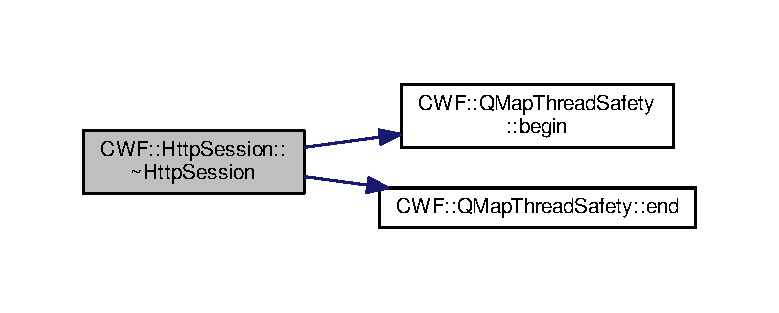
\includegraphics[width=350pt]{class_c_w_f_1_1_http_session_a4bd78eaae88a81643a9e3a911c21759a_cgraph}
\end{center}
\end{figure}




\subsection{Member Function Documentation}
\hypertarget{class_c_w_f_1_1_http_session_a65d09f84231715c5d2cdba2d3aca7626}{\index{C\+W\+F\+::\+Http\+Session@{C\+W\+F\+::\+Http\+Session}!add\+Attribute@{add\+Attribute}}
\index{add\+Attribute@{add\+Attribute}!C\+W\+F\+::\+Http\+Session@{C\+W\+F\+::\+Http\+Session}}
\subsubsection[{add\+Attribute}]{\setlength{\rightskip}{0pt plus 5cm}void C\+W\+F\+::\+Http\+Session\+::add\+Attribute (
\begin{DoxyParamCaption}
\item[{const Q\+String \&}]{name, }
\item[{Q\+Object $\ast$}]{value}
\end{DoxyParamCaption}
)}}\label{class_c_w_f_1_1_http_session_a65d09f84231715c5d2cdba2d3aca7626}


This method add an attribute to the session. 


\begin{DoxyParams}{Parameters}
{\em name} & \\
\hline
{\em value} & \\
\hline
\end{DoxyParams}


Here is the call graph for this function\+:
\nopagebreak
\begin{figure}[H]
\begin{center}
\leavevmode
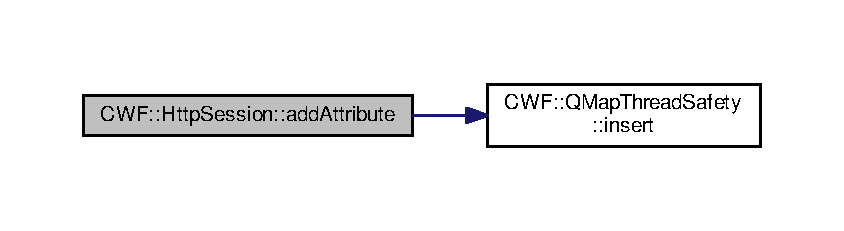
\includegraphics[width=350pt]{class_c_w_f_1_1_http_session_a65d09f84231715c5d2cdba2d3aca7626_cgraph}
\end{center}
\end{figure}


\hypertarget{class_c_w_f_1_1_http_session_a44f59df340395d9c298c93ee5307b392}{\index{C\+W\+F\+::\+Http\+Session@{C\+W\+F\+::\+Http\+Session}!get\+Attribute@{get\+Attribute}}
\index{get\+Attribute@{get\+Attribute}!C\+W\+F\+::\+Http\+Session@{C\+W\+F\+::\+Http\+Session}}
\subsubsection[{get\+Attribute}]{\setlength{\rightskip}{0pt plus 5cm}Q\+Object $\ast$ C\+W\+F\+::\+Http\+Session\+::get\+Attribute (
\begin{DoxyParamCaption}
\item[{const Q\+String \&}]{name}
\end{DoxyParamCaption}
) const}}\label{class_c_w_f_1_1_http_session_a44f59df340395d9c298c93ee5307b392}


get\+Attribute 


\begin{DoxyParams}{Parameters}
{\em name} & \\
\hline
\end{DoxyParams}
\begin{DoxyReturn}{Returns}

\end{DoxyReturn}


Here is the call graph for this function\+:
\nopagebreak
\begin{figure}[H]
\begin{center}
\leavevmode
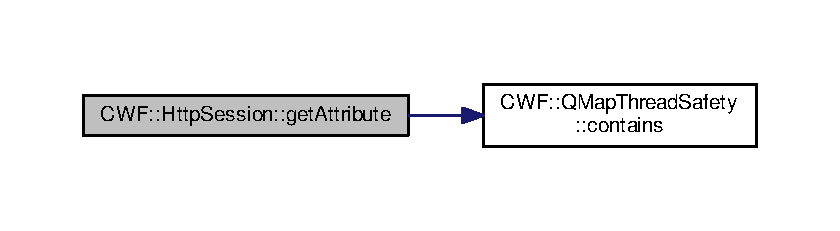
\includegraphics[width=350pt]{class_c_w_f_1_1_http_session_a44f59df340395d9c298c93ee5307b392_cgraph}
\end{center}
\end{figure}


\hypertarget{class_c_w_f_1_1_http_session_a4f7d235f4e4355b6f87179931ced7506}{\index{C\+W\+F\+::\+Http\+Session@{C\+W\+F\+::\+Http\+Session}!get\+Attribute\+Names@{get\+Attribute\+Names}}
\index{get\+Attribute\+Names@{get\+Attribute\+Names}!C\+W\+F\+::\+Http\+Session@{C\+W\+F\+::\+Http\+Session}}
\subsubsection[{get\+Attribute\+Names}]{\setlength{\rightskip}{0pt plus 5cm}Q\+String\+List C\+W\+F\+::\+Http\+Session\+::get\+Attribute\+Names (
\begin{DoxyParamCaption}
{}
\end{DoxyParamCaption}
)}}\label{class_c_w_f_1_1_http_session_a4f7d235f4e4355b6f87179931ced7506}


get\+Attribute\+Names 

\begin{DoxyReturn}{Returns}

\end{DoxyReturn}


Here is the call graph for this function\+:
\nopagebreak
\begin{figure}[H]
\begin{center}
\leavevmode
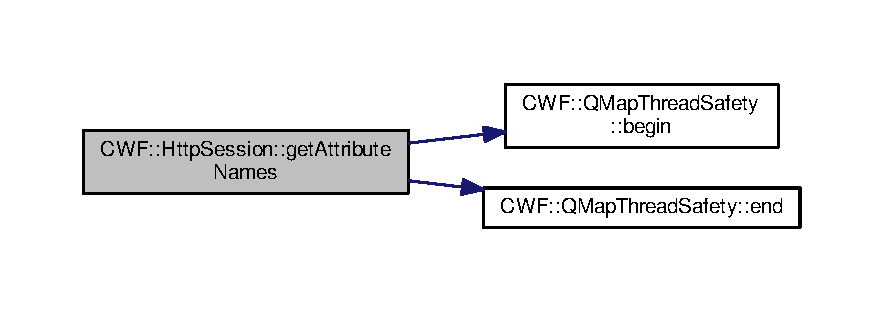
\includegraphics[width=350pt]{class_c_w_f_1_1_http_session_a4f7d235f4e4355b6f87179931ced7506_cgraph}
\end{center}
\end{figure}


\hypertarget{class_c_w_f_1_1_http_session_ae43896253d871a2786ed5a8450b1b644}{\index{C\+W\+F\+::\+Http\+Session@{C\+W\+F\+::\+Http\+Session}!get\+Auto\+Clear\+Attributes@{get\+Auto\+Clear\+Attributes}}
\index{get\+Auto\+Clear\+Attributes@{get\+Auto\+Clear\+Attributes}!C\+W\+F\+::\+Http\+Session@{C\+W\+F\+::\+Http\+Session}}
\subsubsection[{get\+Auto\+Clear\+Attributes}]{\setlength{\rightskip}{0pt plus 5cm}bool C\+W\+F\+::\+Http\+Session\+::get\+Auto\+Clear\+Attributes (
\begin{DoxyParamCaption}
{}
\end{DoxyParamCaption}
) const}}\label{class_c_w_f_1_1_http_session_ae43896253d871a2786ed5a8450b1b644}


get\+Auto\+Clear\+Attributes 

\begin{DoxyReturn}{Returns}
bool 
\end{DoxyReturn}
\hypertarget{class_c_w_f_1_1_http_session_afbb49e2fe7c7f1eb7ea25ec2da21c3dd}{\index{C\+W\+F\+::\+Http\+Session@{C\+W\+F\+::\+Http\+Session}!get\+Creation\+Time@{get\+Creation\+Time}}
\index{get\+Creation\+Time@{get\+Creation\+Time}!C\+W\+F\+::\+Http\+Session@{C\+W\+F\+::\+Http\+Session}}
\subsubsection[{get\+Creation\+Time}]{\setlength{\rightskip}{0pt plus 5cm}qint64 C\+W\+F\+::\+Http\+Session\+::get\+Creation\+Time (
\begin{DoxyParamCaption}
{}
\end{DoxyParamCaption}
) const}}\label{class_c_w_f_1_1_http_session_afbb49e2fe7c7f1eb7ea25ec2da21c3dd}


get\+Creation\+Time 

\begin{DoxyReturn}{Returns}

\end{DoxyReturn}
\hypertarget{class_c_w_f_1_1_http_session_a78aebc496a395e40ab3187e14f4240ed}{\index{C\+W\+F\+::\+Http\+Session@{C\+W\+F\+::\+Http\+Session}!get\+Id@{get\+Id}}
\index{get\+Id@{get\+Id}!C\+W\+F\+::\+Http\+Session@{C\+W\+F\+::\+Http\+Session}}
\subsubsection[{get\+Id}]{\setlength{\rightskip}{0pt plus 5cm}Q\+String C\+W\+F\+::\+Http\+Session\+::get\+Id (
\begin{DoxyParamCaption}
{}
\end{DoxyParamCaption}
) const}}\label{class_c_w_f_1_1_http_session_a78aebc496a395e40ab3187e14f4240ed}


get\+Id 

\begin{DoxyReturn}{Returns}

\end{DoxyReturn}


Here is the caller graph for this function\+:
\nopagebreak
\begin{figure}[H]
\begin{center}
\leavevmode
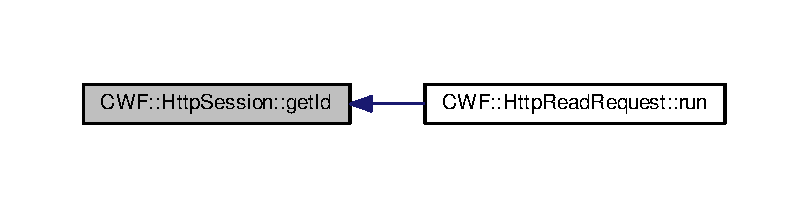
\includegraphics[width=350pt]{class_c_w_f_1_1_http_session_a78aebc496a395e40ab3187e14f4240ed_icgraph}
\end{center}
\end{figure}


\hypertarget{class_c_w_f_1_1_http_session_aa746de987d9c96c1d47005f8135f0aa2}{\index{C\+W\+F\+::\+Http\+Session@{C\+W\+F\+::\+Http\+Session}!get\+Last\+Accessed\+Time@{get\+Last\+Accessed\+Time}}
\index{get\+Last\+Accessed\+Time@{get\+Last\+Accessed\+Time}!C\+W\+F\+::\+Http\+Session@{C\+W\+F\+::\+Http\+Session}}
\subsubsection[{get\+Last\+Accessed\+Time}]{\setlength{\rightskip}{0pt plus 5cm}qint64 C\+W\+F\+::\+Http\+Session\+::get\+Last\+Accessed\+Time (
\begin{DoxyParamCaption}
{}
\end{DoxyParamCaption}
) const}}\label{class_c_w_f_1_1_http_session_aa746de987d9c96c1d47005f8135f0aa2}


get\+Last\+Accessed\+Time 

\begin{DoxyReturn}{Returns}

\end{DoxyReturn}
\hypertarget{class_c_w_f_1_1_http_session_ab8995bcc1581f0116ff73e0496ca8a12}{\index{C\+W\+F\+::\+Http\+Session@{C\+W\+F\+::\+Http\+Session}!invalidate@{invalidate}}
\index{invalidate@{invalidate}!C\+W\+F\+::\+Http\+Session@{C\+W\+F\+::\+Http\+Session}}
\subsubsection[{invalidate}]{\setlength{\rightskip}{0pt plus 5cm}void C\+W\+F\+::\+Http\+Session\+::invalidate (
\begin{DoxyParamCaption}
{}
\end{DoxyParamCaption}
)}}\label{class_c_w_f_1_1_http_session_ab8995bcc1581f0116ff73e0496ca8a12}


invalidate 

\hypertarget{class_c_w_f_1_1_http_session_aebc716e79896ed61527ff4dac933558e}{\index{C\+W\+F\+::\+Http\+Session@{C\+W\+F\+::\+Http\+Session}!is\+Expired@{is\+Expired}}
\index{is\+Expired@{is\+Expired}!C\+W\+F\+::\+Http\+Session@{C\+W\+F\+::\+Http\+Session}}
\subsubsection[{is\+Expired}]{\setlength{\rightskip}{0pt plus 5cm}bool C\+W\+F\+::\+Http\+Session\+::is\+Expired (
\begin{DoxyParamCaption}
{}
\end{DoxyParamCaption}
)}}\label{class_c_w_f_1_1_http_session_aebc716e79896ed61527ff4dac933558e}


This method checks if the session is expired. 

\begin{DoxyReturn}{Returns}
bool 
\end{DoxyReturn}
\hypertarget{class_c_w_f_1_1_http_session_aa2c8fba3e49fd8c43c601d81bf964650}{\index{C\+W\+F\+::\+Http\+Session@{C\+W\+F\+::\+Http\+Session}!remove\+Attribute@{remove\+Attribute}}
\index{remove\+Attribute@{remove\+Attribute}!C\+W\+F\+::\+Http\+Session@{C\+W\+F\+::\+Http\+Session}}
\subsubsection[{remove\+Attribute}]{\setlength{\rightskip}{0pt plus 5cm}void C\+W\+F\+::\+Http\+Session\+::remove\+Attribute (
\begin{DoxyParamCaption}
\item[{const Q\+String \&}]{name}
\end{DoxyParamCaption}
)}}\label{class_c_w_f_1_1_http_session_aa2c8fba3e49fd8c43c601d81bf964650}


remove\+Attribute 


\begin{DoxyParams}{Parameters}
{\em name} & \\
\hline
\end{DoxyParams}


Here is the call graph for this function\+:
\nopagebreak
\begin{figure}[H]
\begin{center}
\leavevmode
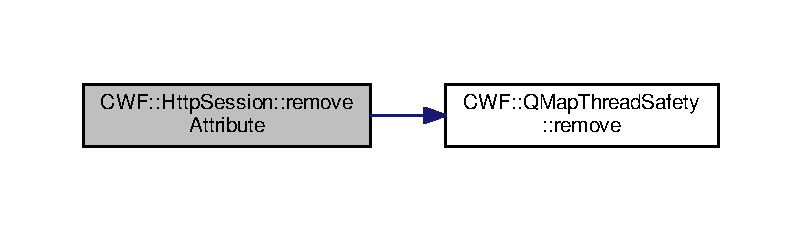
\includegraphics[width=350pt]{class_c_w_f_1_1_http_session_aa2c8fba3e49fd8c43c601d81bf964650_cgraph}
\end{center}
\end{figure}


\hypertarget{class_c_w_f_1_1_http_session_a12f419d327a704a5daf3e53f72671626}{\index{C\+W\+F\+::\+Http\+Session@{C\+W\+F\+::\+Http\+Session}!set\+Auto\+Clear\+Attributes@{set\+Auto\+Clear\+Attributes}}
\index{set\+Auto\+Clear\+Attributes@{set\+Auto\+Clear\+Attributes}!C\+W\+F\+::\+Http\+Session@{C\+W\+F\+::\+Http\+Session}}
\subsubsection[{set\+Auto\+Clear\+Attributes}]{\setlength{\rightskip}{0pt plus 5cm}void C\+W\+F\+::\+Http\+Session\+::set\+Auto\+Clear\+Attributes (
\begin{DoxyParamCaption}
\item[{bool}]{value}
\end{DoxyParamCaption}
)}}\label{class_c_w_f_1_1_http_session_a12f419d327a704a5daf3e53f72671626}


set\+Auto\+Clear\+Attributes 


\begin{DoxyParams}{Parameters}
{\em value} & \\
\hline
\end{DoxyParams}
\hypertarget{class_c_w_f_1_1_http_session_a9702d3c0b959cb59aac53d9eb9a05fd7}{\index{C\+W\+F\+::\+Http\+Session@{C\+W\+F\+::\+Http\+Session}!validate@{validate}}
\index{validate@{validate}!C\+W\+F\+::\+Http\+Session@{C\+W\+F\+::\+Http\+Session}}
\subsubsection[{validate}]{\setlength{\rightskip}{0pt plus 5cm}void C\+W\+F\+::\+Http\+Session\+::validate (
\begin{DoxyParamCaption}
{}
\end{DoxyParamCaption}
)}}\label{class_c_w_f_1_1_http_session_a9702d3c0b959cb59aac53d9eb9a05fd7}


validate 



\subsection{Friends And Related Function Documentation}
\hypertarget{class_c_w_f_1_1_http_session_a4d54f5003e07e218070a449c22a52c7c}{\index{C\+W\+F\+::\+Http\+Session@{C\+W\+F\+::\+Http\+Session}!Http\+Read\+Request@{Http\+Read\+Request}}
\index{Http\+Read\+Request@{Http\+Read\+Request}!C\+W\+F\+::\+Http\+Session@{C\+W\+F\+::\+Http\+Session}}
\subsubsection[{Http\+Read\+Request}]{\setlength{\rightskip}{0pt plus 5cm}friend class {\bf Http\+Read\+Request}\hspace{0.3cm}{\ttfamily [friend]}}}\label{class_c_w_f_1_1_http_session_a4d54f5003e07e218070a449c22a52c7c}


The documentation for this class was generated from the following files\+:\begin{DoxyCompactItemize}
\item 
/home/herik/\+C\+P\+P\+Web\+Framework/\+C\+P\+P\+Web\+Framework/cwf/\hyperlink{httpsession_8h}{httpsession.\+h}\item 
/home/herik/\+C\+P\+P\+Web\+Framework/\+C\+P\+P\+Web\+Framework/cwf/\hyperlink{httpsession_8cpp}{httpsession.\+cpp}\end{DoxyCompactItemize}

\hypertarget{class_c_w_f_1_1_if_attributes}{\section{C\+W\+F\+:\+:If\+Attributes Class Reference}
\label{class_c_w_f_1_1_if_attributes}\index{C\+W\+F\+::\+If\+Attributes@{C\+W\+F\+::\+If\+Attributes}}
}


{\ttfamily \#include $<$ifattributes.\+h$>$}

\subsection*{Public Member Functions}
\begin{DoxyCompactItemize}
\item 
\hyperlink{class_c_w_f_1_1_if_attributes_abbb26ca2878fade9ad1dc6cfb3f94ac1}{If\+Attributes} (const Q\+Xml\+Stream\+Attributes \&attributes)
\end{DoxyCompactItemize}
\subsection*{Public Attributes}
\begin{DoxyCompactItemize}
\item 
Q\+String \hyperlink{class_c_w_f_1_1_if_attributes_a57a2a9012c72fb354b2bf1e30f2bd832}{var}
\item 
Q\+String \hyperlink{class_c_w_f_1_1_if_attributes_a514ef0fbe32a7c2ea5aba6218f182477}{equal}
\item 
Q\+String \hyperlink{class_c_w_f_1_1_if_attributes_aebb39701f4b50e474998c95d099ac977}{not\+Equal}
\item 
Q\+String \hyperlink{class_c_w_f_1_1_if_attributes_a19ce01e769f9a51eb087e20b05f9e2f3}{greater}
\item 
Q\+String \hyperlink{class_c_w_f_1_1_if_attributes_a16843cddaa8d16acf67a31a1258826d5}{less}
\item 
Q\+String \hyperlink{class_c_w_f_1_1_if_attributes_aae911ff049668fedc849435c466891ac}{greater\+Equal}
\item 
Q\+String \hyperlink{class_c_w_f_1_1_if_attributes_aea6e443b32ec1deaf0d0f7025d49b9b2}{less\+Equal}
\item 
Q\+String \hyperlink{class_c_w_f_1_1_if_attributes_acde13fdcb70d1667f96b197762349d54}{error}
\item 
bool \hyperlink{class_c_w_f_1_1_if_attributes_a333a69fcd0b5c9cc450e5f1a9c0434cb}{condition} = false
\end{DoxyCompactItemize}


\subsection{Constructor \& Destructor Documentation}
\hypertarget{class_c_w_f_1_1_if_attributes_abbb26ca2878fade9ad1dc6cfb3f94ac1}{\index{C\+W\+F\+::\+If\+Attributes@{C\+W\+F\+::\+If\+Attributes}!If\+Attributes@{If\+Attributes}}
\index{If\+Attributes@{If\+Attributes}!C\+W\+F\+::\+If\+Attributes@{C\+W\+F\+::\+If\+Attributes}}
\subsubsection[{If\+Attributes}]{\setlength{\rightskip}{0pt plus 5cm}C\+W\+F\+::\+If\+Attributes\+::\+If\+Attributes (
\begin{DoxyParamCaption}
\item[{const Q\+Xml\+Stream\+Attributes \&}]{attributes}
\end{DoxyParamCaption}
)}}\label{class_c_w_f_1_1_if_attributes_abbb26ca2878fade9ad1dc6cfb3f94ac1}


\subsection{Member Data Documentation}
\hypertarget{class_c_w_f_1_1_if_attributes_a333a69fcd0b5c9cc450e5f1a9c0434cb}{\index{C\+W\+F\+::\+If\+Attributes@{C\+W\+F\+::\+If\+Attributes}!condition@{condition}}
\index{condition@{condition}!C\+W\+F\+::\+If\+Attributes@{C\+W\+F\+::\+If\+Attributes}}
\subsubsection[{condition}]{\setlength{\rightskip}{0pt plus 5cm}bool C\+W\+F\+::\+If\+Attributes\+::condition = false}}\label{class_c_w_f_1_1_if_attributes_a333a69fcd0b5c9cc450e5f1a9c0434cb}
\hypertarget{class_c_w_f_1_1_if_attributes_a514ef0fbe32a7c2ea5aba6218f182477}{\index{C\+W\+F\+::\+If\+Attributes@{C\+W\+F\+::\+If\+Attributes}!equal@{equal}}
\index{equal@{equal}!C\+W\+F\+::\+If\+Attributes@{C\+W\+F\+::\+If\+Attributes}}
\subsubsection[{equal}]{\setlength{\rightskip}{0pt plus 5cm}Q\+String C\+W\+F\+::\+If\+Attributes\+::equal}}\label{class_c_w_f_1_1_if_attributes_a514ef0fbe32a7c2ea5aba6218f182477}
\hypertarget{class_c_w_f_1_1_if_attributes_acde13fdcb70d1667f96b197762349d54}{\index{C\+W\+F\+::\+If\+Attributes@{C\+W\+F\+::\+If\+Attributes}!error@{error}}
\index{error@{error}!C\+W\+F\+::\+If\+Attributes@{C\+W\+F\+::\+If\+Attributes}}
\subsubsection[{error}]{\setlength{\rightskip}{0pt plus 5cm}Q\+String C\+W\+F\+::\+If\+Attributes\+::error}}\label{class_c_w_f_1_1_if_attributes_acde13fdcb70d1667f96b197762349d54}
\hypertarget{class_c_w_f_1_1_if_attributes_a19ce01e769f9a51eb087e20b05f9e2f3}{\index{C\+W\+F\+::\+If\+Attributes@{C\+W\+F\+::\+If\+Attributes}!greater@{greater}}
\index{greater@{greater}!C\+W\+F\+::\+If\+Attributes@{C\+W\+F\+::\+If\+Attributes}}
\subsubsection[{greater}]{\setlength{\rightskip}{0pt plus 5cm}Q\+String C\+W\+F\+::\+If\+Attributes\+::greater}}\label{class_c_w_f_1_1_if_attributes_a19ce01e769f9a51eb087e20b05f9e2f3}
\hypertarget{class_c_w_f_1_1_if_attributes_aae911ff049668fedc849435c466891ac}{\index{C\+W\+F\+::\+If\+Attributes@{C\+W\+F\+::\+If\+Attributes}!greater\+Equal@{greater\+Equal}}
\index{greater\+Equal@{greater\+Equal}!C\+W\+F\+::\+If\+Attributes@{C\+W\+F\+::\+If\+Attributes}}
\subsubsection[{greater\+Equal}]{\setlength{\rightskip}{0pt plus 5cm}Q\+String C\+W\+F\+::\+If\+Attributes\+::greater\+Equal}}\label{class_c_w_f_1_1_if_attributes_aae911ff049668fedc849435c466891ac}
\hypertarget{class_c_w_f_1_1_if_attributes_a16843cddaa8d16acf67a31a1258826d5}{\index{C\+W\+F\+::\+If\+Attributes@{C\+W\+F\+::\+If\+Attributes}!less@{less}}
\index{less@{less}!C\+W\+F\+::\+If\+Attributes@{C\+W\+F\+::\+If\+Attributes}}
\subsubsection[{less}]{\setlength{\rightskip}{0pt plus 5cm}Q\+String C\+W\+F\+::\+If\+Attributes\+::less}}\label{class_c_w_f_1_1_if_attributes_a16843cddaa8d16acf67a31a1258826d5}
\hypertarget{class_c_w_f_1_1_if_attributes_aea6e443b32ec1deaf0d0f7025d49b9b2}{\index{C\+W\+F\+::\+If\+Attributes@{C\+W\+F\+::\+If\+Attributes}!less\+Equal@{less\+Equal}}
\index{less\+Equal@{less\+Equal}!C\+W\+F\+::\+If\+Attributes@{C\+W\+F\+::\+If\+Attributes}}
\subsubsection[{less\+Equal}]{\setlength{\rightskip}{0pt plus 5cm}Q\+String C\+W\+F\+::\+If\+Attributes\+::less\+Equal}}\label{class_c_w_f_1_1_if_attributes_aea6e443b32ec1deaf0d0f7025d49b9b2}
\hypertarget{class_c_w_f_1_1_if_attributes_aebb39701f4b50e474998c95d099ac977}{\index{C\+W\+F\+::\+If\+Attributes@{C\+W\+F\+::\+If\+Attributes}!not\+Equal@{not\+Equal}}
\index{not\+Equal@{not\+Equal}!C\+W\+F\+::\+If\+Attributes@{C\+W\+F\+::\+If\+Attributes}}
\subsubsection[{not\+Equal}]{\setlength{\rightskip}{0pt plus 5cm}Q\+String C\+W\+F\+::\+If\+Attributes\+::not\+Equal}}\label{class_c_w_f_1_1_if_attributes_aebb39701f4b50e474998c95d099ac977}
\hypertarget{class_c_w_f_1_1_if_attributes_a57a2a9012c72fb354b2bf1e30f2bd832}{\index{C\+W\+F\+::\+If\+Attributes@{C\+W\+F\+::\+If\+Attributes}!var@{var}}
\index{var@{var}!C\+W\+F\+::\+If\+Attributes@{C\+W\+F\+::\+If\+Attributes}}
\subsubsection[{var}]{\setlength{\rightskip}{0pt plus 5cm}Q\+String C\+W\+F\+::\+If\+Attributes\+::var}}\label{class_c_w_f_1_1_if_attributes_a57a2a9012c72fb354b2bf1e30f2bd832}


The documentation for this class was generated from the following files\+:\begin{DoxyCompactItemize}
\item 
/home/herik/\+C\+P\+P\+Web\+Framework/\+C\+P\+P\+Web\+Framework/cwf/\hyperlink{ifattributes_8h}{ifattributes.\+h}\item 
/home/herik/\+C\+P\+P\+Web\+Framework/\+C\+P\+P\+Web\+Framework/cwf/\hyperlink{ifattributes_8cpp}{ifattributes.\+cpp}\end{DoxyCompactItemize}

\hypertarget{class_c_w_f_1_1_meta_class_parser}{\section{C\+W\+F\+:\+:Meta\+Class\+Parser Class Reference}
\label{class_c_w_f_1_1_meta_class_parser}\index{C\+W\+F\+::\+Meta\+Class\+Parser@{C\+W\+F\+::\+Meta\+Class\+Parser}}
}


{\ttfamily \#include $<$metaclassparser.\+h$>$}

\subsection*{Public Member Functions}
\begin{DoxyCompactItemize}
\item 
\hyperlink{class_c_w_f_1_1_meta_class_parser_af831499a518f79c328a71d8d8ec53b0f}{Meta\+Class\+Parser} (Q\+Object $\ast$object)
\item 
Q\+String \hyperlink{class_c_w_f_1_1_meta_class_parser_a2bd37870867411d803411339d1d97c49}{get\+Return\+Type} (const Q\+String \&method\+Name)
\item 
Q\+String \hyperlink{class_c_w_f_1_1_meta_class_parser_a560be3a1d52f822eab715faa0b1fbe15}{get\+Parameter\+Type} (const Q\+String \&method\+Name)
\end{DoxyCompactItemize}
\subsection*{Static Public Member Functions}
\begin{DoxyCompactItemize}
\item 
static void $\ast$ \hyperlink{class_c_w_f_1_1_meta_class_parser_a0d9a5f5b026f0fc7e257fa58bbc72adf}{instantiate\+Class\+By\+Name} (const Q\+Byte\+Array \&name)
\end{DoxyCompactItemize}
\subsection*{Public Attributes}
\begin{DoxyCompactItemize}
\item 
Q\+Map$<$ std\+::tuple$<$ Q\+String, \\*
Q\+String $>$, Q\+Meta\+Method $>$ \hyperlink{class_c_w_f_1_1_meta_class_parser_a39c54c4665716493927f2e36be0c2cc9}{methods}
\item 
Q\+Map$<$ Q\+String, Q\+Meta\+Property $>$ \hyperlink{class_c_w_f_1_1_meta_class_parser_a24721c126dfff6fba83a4d5dd088ee69}{properties}
\end{DoxyCompactItemize}


\subsection{Constructor \& Destructor Documentation}
\hypertarget{class_c_w_f_1_1_meta_class_parser_af831499a518f79c328a71d8d8ec53b0f}{\index{C\+W\+F\+::\+Meta\+Class\+Parser@{C\+W\+F\+::\+Meta\+Class\+Parser}!Meta\+Class\+Parser@{Meta\+Class\+Parser}}
\index{Meta\+Class\+Parser@{Meta\+Class\+Parser}!C\+W\+F\+::\+Meta\+Class\+Parser@{C\+W\+F\+::\+Meta\+Class\+Parser}}
\subsubsection[{Meta\+Class\+Parser}]{\setlength{\rightskip}{0pt plus 5cm}C\+W\+F\+::\+Meta\+Class\+Parser\+::\+Meta\+Class\+Parser (
\begin{DoxyParamCaption}
\item[{Q\+Object $\ast$}]{object}
\end{DoxyParamCaption}
)\hspace{0.3cm}{\ttfamily [explicit]}}}\label{class_c_w_f_1_1_meta_class_parser_af831499a518f79c328a71d8d8ec53b0f}


\subsection{Member Function Documentation}
\hypertarget{class_c_w_f_1_1_meta_class_parser_a560be3a1d52f822eab715faa0b1fbe15}{\index{C\+W\+F\+::\+Meta\+Class\+Parser@{C\+W\+F\+::\+Meta\+Class\+Parser}!get\+Parameter\+Type@{get\+Parameter\+Type}}
\index{get\+Parameter\+Type@{get\+Parameter\+Type}!C\+W\+F\+::\+Meta\+Class\+Parser@{C\+W\+F\+::\+Meta\+Class\+Parser}}
\subsubsection[{get\+Parameter\+Type}]{\setlength{\rightskip}{0pt plus 5cm}Q\+String C\+W\+F\+::\+Meta\+Class\+Parser\+::get\+Parameter\+Type (
\begin{DoxyParamCaption}
\item[{const Q\+String \&}]{method\+Name}
\end{DoxyParamCaption}
)}}\label{class_c_w_f_1_1_meta_class_parser_a560be3a1d52f822eab715faa0b1fbe15}


Here is the caller graph for this function\+:
\nopagebreak
\begin{figure}[H]
\begin{center}
\leavevmode
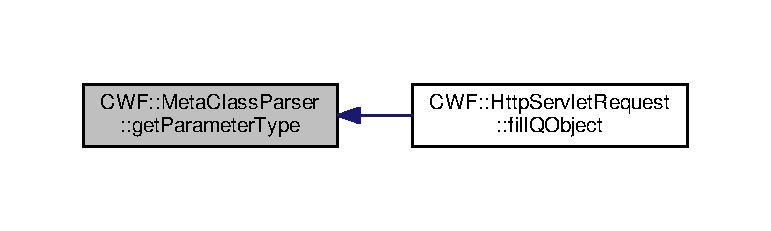
\includegraphics[width=350pt]{class_c_w_f_1_1_meta_class_parser_a560be3a1d52f822eab715faa0b1fbe15_icgraph}
\end{center}
\end{figure}


\hypertarget{class_c_w_f_1_1_meta_class_parser_a2bd37870867411d803411339d1d97c49}{\index{C\+W\+F\+::\+Meta\+Class\+Parser@{C\+W\+F\+::\+Meta\+Class\+Parser}!get\+Return\+Type@{get\+Return\+Type}}
\index{get\+Return\+Type@{get\+Return\+Type}!C\+W\+F\+::\+Meta\+Class\+Parser@{C\+W\+F\+::\+Meta\+Class\+Parser}}
\subsubsection[{get\+Return\+Type}]{\setlength{\rightskip}{0pt plus 5cm}Q\+String C\+W\+F\+::\+Meta\+Class\+Parser\+::get\+Return\+Type (
\begin{DoxyParamCaption}
\item[{const Q\+String \&}]{method\+Name}
\end{DoxyParamCaption}
)}}\label{class_c_w_f_1_1_meta_class_parser_a2bd37870867411d803411339d1d97c49}


Here is the caller graph for this function\+:
\nopagebreak
\begin{figure}[H]
\begin{center}
\leavevmode
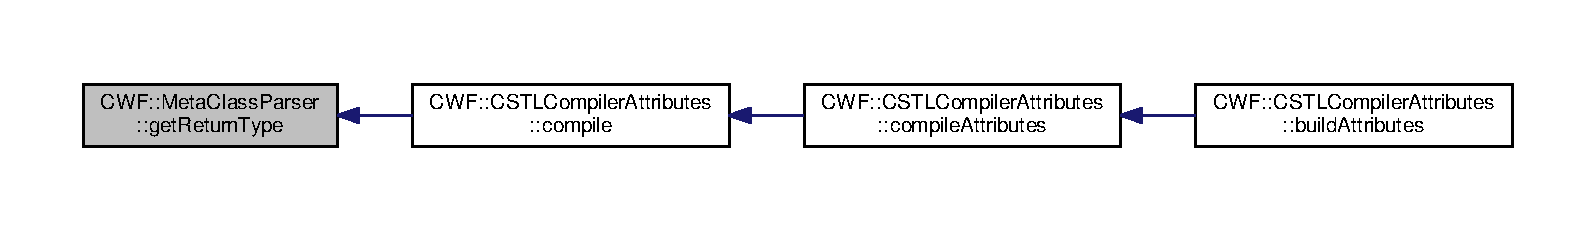
\includegraphics[width=350pt]{class_c_w_f_1_1_meta_class_parser_a2bd37870867411d803411339d1d97c49_icgraph}
\end{center}
\end{figure}


\hypertarget{class_c_w_f_1_1_meta_class_parser_a0d9a5f5b026f0fc7e257fa58bbc72adf}{\index{C\+W\+F\+::\+Meta\+Class\+Parser@{C\+W\+F\+::\+Meta\+Class\+Parser}!instantiate\+Class\+By\+Name@{instantiate\+Class\+By\+Name}}
\index{instantiate\+Class\+By\+Name@{instantiate\+Class\+By\+Name}!C\+W\+F\+::\+Meta\+Class\+Parser@{C\+W\+F\+::\+Meta\+Class\+Parser}}
\subsubsection[{instantiate\+Class\+By\+Name}]{\setlength{\rightskip}{0pt plus 5cm}void $\ast$ C\+W\+F\+::\+Meta\+Class\+Parser\+::instantiate\+Class\+By\+Name (
\begin{DoxyParamCaption}
\item[{const Q\+Byte\+Array \&}]{name}
\end{DoxyParamCaption}
)\hspace{0.3cm}{\ttfamily [static]}}}\label{class_c_w_f_1_1_meta_class_parser_a0d9a5f5b026f0fc7e257fa58bbc72adf}


\subsection{Member Data Documentation}
\hypertarget{class_c_w_f_1_1_meta_class_parser_a39c54c4665716493927f2e36be0c2cc9}{\index{C\+W\+F\+::\+Meta\+Class\+Parser@{C\+W\+F\+::\+Meta\+Class\+Parser}!methods@{methods}}
\index{methods@{methods}!C\+W\+F\+::\+Meta\+Class\+Parser@{C\+W\+F\+::\+Meta\+Class\+Parser}}
\subsubsection[{methods}]{\setlength{\rightskip}{0pt plus 5cm}Q\+Map$<$std\+::tuple$<$Q\+String, Q\+String$>$, Q\+Meta\+Method$>$ C\+W\+F\+::\+Meta\+Class\+Parser\+::methods}}\label{class_c_w_f_1_1_meta_class_parser_a39c54c4665716493927f2e36be0c2cc9}
\hypertarget{class_c_w_f_1_1_meta_class_parser_a24721c126dfff6fba83a4d5dd088ee69}{\index{C\+W\+F\+::\+Meta\+Class\+Parser@{C\+W\+F\+::\+Meta\+Class\+Parser}!properties@{properties}}
\index{properties@{properties}!C\+W\+F\+::\+Meta\+Class\+Parser@{C\+W\+F\+::\+Meta\+Class\+Parser}}
\subsubsection[{properties}]{\setlength{\rightskip}{0pt plus 5cm}Q\+Map$<$Q\+String, Q\+Meta\+Property$>$ C\+W\+F\+::\+Meta\+Class\+Parser\+::properties}}\label{class_c_w_f_1_1_meta_class_parser_a24721c126dfff6fba83a4d5dd088ee69}


The documentation for this class was generated from the following files\+:\begin{DoxyCompactItemize}
\item 
/home/herik/\+C\+P\+P\+Web\+Framework/\+C\+P\+P\+Web\+Framework/cwf/\hyperlink{metaclassparser_8h}{metaclassparser.\+h}\item 
/home/herik/\+C\+P\+P\+Web\+Framework/\+C\+P\+P\+Web\+Framework/cwf/\hyperlink{metaclassparser_8cpp}{metaclassparser.\+cpp}\end{DoxyCompactItemize}

\hypertarget{class_c_w_f_1_1_properties}{\section{C\+W\+F\+:\+:Properties Class Reference}
\label{class_c_w_f_1_1_properties}\index{C\+W\+F\+::\+Properties@{C\+W\+F\+::\+Properties}}
}


The \hyperlink{class_c_w_f_1_1_properties}{Properties} class is an auxiliar class to the \hyperlink{class_c_w_f_1_1_c_s_t_l_compiler}{C\+S\+T\+L\+Compiler}.  




{\ttfamily \#include $<$properties.\+h$>$}

\subsection*{Public Member Functions}
\begin{DoxyCompactItemize}
\item 
\hyperlink{class_c_w_f_1_1_properties_a417638a2312fba16104f19bc59190b35}{Properties} ()=default
\item 
\hyperlink{class_c_w_f_1_1_properties_ad37244d75ca8ae82b8122b2f5d6952a2}{Properties} (const Q\+String \&class\+And\+Method)
\end{DoxyCompactItemize}
\subsection*{Public Attributes}
\begin{DoxyCompactItemize}
\item 
Q\+String \hyperlink{class_c_w_f_1_1_properties_ad77aa99c8e2ea4afe6300d739ba22308}{m\+\_\+class}
\item 
Q\+String \hyperlink{class_c_w_f_1_1_properties_a70682c472acdeef56e50a79f2436833e}{m\+\_\+method}
\end{DoxyCompactItemize}


\subsection{Detailed Description}
The \hyperlink{class_c_w_f_1_1_properties}{Properties} class is an auxiliar class to the \hyperlink{class_c_w_f_1_1_c_s_t_l_compiler}{C\+S\+T\+L\+Compiler}. 

\subsection{Constructor \& Destructor Documentation}
\hypertarget{class_c_w_f_1_1_properties_a417638a2312fba16104f19bc59190b35}{\index{C\+W\+F\+::\+Properties@{C\+W\+F\+::\+Properties}!Properties@{Properties}}
\index{Properties@{Properties}!C\+W\+F\+::\+Properties@{C\+W\+F\+::\+Properties}}
\subsubsection[{Properties}]{\setlength{\rightskip}{0pt plus 5cm}C\+W\+F\+::\+Properties\+::\+Properties (
\begin{DoxyParamCaption}
{}
\end{DoxyParamCaption}
)\hspace{0.3cm}{\ttfamily [default]}}}\label{class_c_w_f_1_1_properties_a417638a2312fba16104f19bc59190b35}
\hypertarget{class_c_w_f_1_1_properties_ad37244d75ca8ae82b8122b2f5d6952a2}{\index{C\+W\+F\+::\+Properties@{C\+W\+F\+::\+Properties}!Properties@{Properties}}
\index{Properties@{Properties}!C\+W\+F\+::\+Properties@{C\+W\+F\+::\+Properties}}
\subsubsection[{Properties}]{\setlength{\rightskip}{0pt plus 5cm}C\+W\+F\+::\+Properties\+::\+Properties (
\begin{DoxyParamCaption}
\item[{const Q\+String \&}]{class\+And\+Method}
\end{DoxyParamCaption}
)\hspace{0.3cm}{\ttfamily [inline]}}}\label{class_c_w_f_1_1_properties_ad37244d75ca8ae82b8122b2f5d6952a2}


\subsection{Member Data Documentation}
\hypertarget{class_c_w_f_1_1_properties_ad77aa99c8e2ea4afe6300d739ba22308}{\index{C\+W\+F\+::\+Properties@{C\+W\+F\+::\+Properties}!m\+\_\+class@{m\+\_\+class}}
\index{m\+\_\+class@{m\+\_\+class}!C\+W\+F\+::\+Properties@{C\+W\+F\+::\+Properties}}
\subsubsection[{m\+\_\+class}]{\setlength{\rightskip}{0pt plus 5cm}Q\+String C\+W\+F\+::\+Properties\+::m\+\_\+class}}\label{class_c_w_f_1_1_properties_ad77aa99c8e2ea4afe6300d739ba22308}
\hypertarget{class_c_w_f_1_1_properties_a70682c472acdeef56e50a79f2436833e}{\index{C\+W\+F\+::\+Properties@{C\+W\+F\+::\+Properties}!m\+\_\+method@{m\+\_\+method}}
\index{m\+\_\+method@{m\+\_\+method}!C\+W\+F\+::\+Properties@{C\+W\+F\+::\+Properties}}
\subsubsection[{m\+\_\+method}]{\setlength{\rightskip}{0pt plus 5cm}Q\+String C\+W\+F\+::\+Properties\+::m\+\_\+method}}\label{class_c_w_f_1_1_properties_a70682c472acdeef56e50a79f2436833e}


The documentation for this class was generated from the following file\+:\begin{DoxyCompactItemize}
\item 
/home/herik/\+C\+P\+P\+Web\+Framework/\+C\+P\+P\+Web\+Framework/cwf/\hyperlink{properties_8h}{properties.\+h}\end{DoxyCompactItemize}

\hypertarget{class_c_w_f_1_1_q_list_object}{\section{C\+W\+F\+:\+:Q\+List\+Object Class Reference}
\label{class_c_w_f_1_1_q_list_object}\index{C\+W\+F\+::\+Q\+List\+Object@{C\+W\+F\+::\+Q\+List\+Object}}
}


The \hyperlink{class_c_w_f_1_1_q_list_object}{Q\+List\+Object} class is used to pass a list of object to a xhtml page. N\+O\+T\+E\+: Always when you need to pass a list of object to a xhtml page you will need to use this class, your class need to inherit from the Q\+Object class and all the methods needs to be in the public slots session.  




{\ttfamily \#include $<$qlistobject.\+h$>$}



Inheritance diagram for C\+W\+F\+:\+:Q\+List\+Object\+:
\nopagebreak
\begin{figure}[H]
\begin{center}
\leavevmode
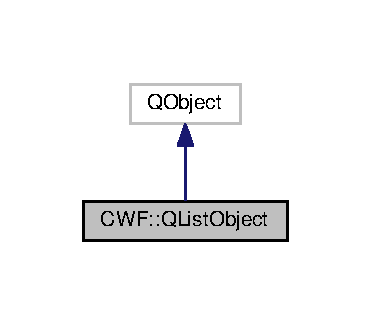
\includegraphics[width=178pt]{class_c_w_f_1_1_q_list_object__inherit__graph}
\end{center}
\end{figure}
\subsection*{Public Member Functions}
\begin{DoxyCompactItemize}
\item 
\hyperlink{class_c_w_f_1_1_q_list_object_a6b056337424f80209ceabb4a3e13b9f8}{Q\+List\+Object} (Q\+Object $\ast$parent=0)
\begin{DoxyCompactList}\small\item\em This constructor can receive a parent. \end{DoxyCompactList}\item 
\hyperlink{class_c_w_f_1_1_q_list_object_a9d1a062c955dad25d5b6261d73f6c87c}{$\sim$\+Q\+List\+Object} ()
\item 
Q\+Object $\ast$ \hyperlink{class_c_w_f_1_1_q_list_object_a987e849c926c80558272f6d0fc019fae}{operator\mbox{[}$\,$\mbox{]}} (int index) const 
\begin{DoxyCompactList}\small\item\em This is an operator overload and returns a Q\+Object given an specific index. \end{DoxyCompactList}\item 
int \hyperlink{class_c_w_f_1_1_q_list_object_a2de65b58fcc28b3d40de2af763b5e6f4}{size} () const 
\begin{DoxyCompactList}\small\item\em This method returns the number of elements in this \hyperlink{class_c_w_f_1_1_q_list_object}{Q\+List\+Object}. \end{DoxyCompactList}\item 
void \hyperlink{class_c_w_f_1_1_q_list_object_ac05809bbe119d6d4964efd721d0bef3a}{add} (Q\+Object $\ast$object)
\begin{DoxyCompactList}\small\item\em This method add a new Q\+Object to the list. \end{DoxyCompactList}\item 
void \hyperlink{class_c_w_f_1_1_q_list_object_a4d8b3e00c8ee8add45a473582ec0253b}{remove} (Q\+Object $\ast$object)
\begin{DoxyCompactList}\small\item\em This method remove. \end{DoxyCompactList}\item 
bool \hyperlink{class_c_w_f_1_1_q_list_object_a8154d32ef214c0e765aebd29cc284572}{get\+Auto\+Delete} () const 
\item 
void \hyperlink{class_c_w_f_1_1_q_list_object_aefb8c78635548e4fba6e47449d47353c}{set\+Auto\+Delete} (bool value)
\end{DoxyCompactItemize}


\subsection{Detailed Description}
The \hyperlink{class_c_w_f_1_1_q_list_object}{Q\+List\+Object} class is used to pass a list of object to a xhtml page. N\+O\+T\+E\+: Always when you need to pass a list of object to a xhtml page you will need to use this class, your class need to inherit from the Q\+Object class and all the methods needs to be in the public slots session. 

\subsection{Constructor \& Destructor Documentation}
\hypertarget{class_c_w_f_1_1_q_list_object_a6b056337424f80209ceabb4a3e13b9f8}{\index{C\+W\+F\+::\+Q\+List\+Object@{C\+W\+F\+::\+Q\+List\+Object}!Q\+List\+Object@{Q\+List\+Object}}
\index{Q\+List\+Object@{Q\+List\+Object}!C\+W\+F\+::\+Q\+List\+Object@{C\+W\+F\+::\+Q\+List\+Object}}
\subsubsection[{Q\+List\+Object}]{\setlength{\rightskip}{0pt plus 5cm}C\+W\+F\+::\+Q\+List\+Object\+::\+Q\+List\+Object (
\begin{DoxyParamCaption}
\item[{Q\+Object $\ast$}]{parent = {\ttfamily 0}}
\end{DoxyParamCaption}
)\hspace{0.3cm}{\ttfamily [explicit]}}}\label{class_c_w_f_1_1_q_list_object_a6b056337424f80209ceabb4a3e13b9f8}


This constructor can receive a parent. 


\begin{DoxyParams}{Parameters}
{\em parent()} & \+: This is a pointer to a Q\+Object. \\
\hline
\end{DoxyParams}
\hypertarget{class_c_w_f_1_1_q_list_object_a9d1a062c955dad25d5b6261d73f6c87c}{\index{C\+W\+F\+::\+Q\+List\+Object@{C\+W\+F\+::\+Q\+List\+Object}!````~Q\+List\+Object@{$\sim$\+Q\+List\+Object}}
\index{````~Q\+List\+Object@{$\sim$\+Q\+List\+Object}!C\+W\+F\+::\+Q\+List\+Object@{C\+W\+F\+::\+Q\+List\+Object}}
\subsubsection[{$\sim$\+Q\+List\+Object}]{\setlength{\rightskip}{0pt plus 5cm}C\+W\+F\+::\+Q\+List\+Object\+::$\sim$\+Q\+List\+Object (
\begin{DoxyParamCaption}
{}
\end{DoxyParamCaption}
)}}\label{class_c_w_f_1_1_q_list_object_a9d1a062c955dad25d5b6261d73f6c87c}


\subsection{Member Function Documentation}
\hypertarget{class_c_w_f_1_1_q_list_object_ac05809bbe119d6d4964efd721d0bef3a}{\index{C\+W\+F\+::\+Q\+List\+Object@{C\+W\+F\+::\+Q\+List\+Object}!add@{add}}
\index{add@{add}!C\+W\+F\+::\+Q\+List\+Object@{C\+W\+F\+::\+Q\+List\+Object}}
\subsubsection[{add}]{\setlength{\rightskip}{0pt plus 5cm}void C\+W\+F\+::\+Q\+List\+Object\+::add (
\begin{DoxyParamCaption}
\item[{Q\+Object $\ast$}]{object}
\end{DoxyParamCaption}
)}}\label{class_c_w_f_1_1_q_list_object_ac05809bbe119d6d4964efd721d0bef3a}


This method add a new Q\+Object to the list. 


\begin{DoxyParams}{Parameters}
{\em o} & \+: This is a pointer to a Q\+Object. \\
\hline
\end{DoxyParams}
\hypertarget{class_c_w_f_1_1_q_list_object_a8154d32ef214c0e765aebd29cc284572}{\index{C\+W\+F\+::\+Q\+List\+Object@{C\+W\+F\+::\+Q\+List\+Object}!get\+Auto\+Delete@{get\+Auto\+Delete}}
\index{get\+Auto\+Delete@{get\+Auto\+Delete}!C\+W\+F\+::\+Q\+List\+Object@{C\+W\+F\+::\+Q\+List\+Object}}
\subsubsection[{get\+Auto\+Delete}]{\setlength{\rightskip}{0pt plus 5cm}bool C\+W\+F\+::\+Q\+List\+Object\+::get\+Auto\+Delete (
\begin{DoxyParamCaption}
{}
\end{DoxyParamCaption}
) const}}\label{class_c_w_f_1_1_q_list_object_a8154d32ef214c0e765aebd29cc284572}
\hypertarget{class_c_w_f_1_1_q_list_object_a987e849c926c80558272f6d0fc019fae}{\index{C\+W\+F\+::\+Q\+List\+Object@{C\+W\+F\+::\+Q\+List\+Object}!operator\mbox{[}$\,$\mbox{]}@{operator[]}}
\index{operator\mbox{[}$\,$\mbox{]}@{operator[]}!C\+W\+F\+::\+Q\+List\+Object@{C\+W\+F\+::\+Q\+List\+Object}}
\subsubsection[{operator[]}]{\setlength{\rightskip}{0pt plus 5cm}Q\+Object $\ast$ C\+W\+F\+::\+Q\+List\+Object\+::operator\mbox{[}$\,$\mbox{]} (
\begin{DoxyParamCaption}
\item[{int}]{index}
\end{DoxyParamCaption}
) const}}\label{class_c_w_f_1_1_q_list_object_a987e849c926c80558272f6d0fc019fae}


This is an operator overload and returns a Q\+Object given an specific index. 


\begin{DoxyParams}{Parameters}
{\em index} & \+: This is an integer value. \\
\hline
\end{DoxyParams}
\begin{DoxyReturn}{Returns}
Q\+Object $\ast$ 
\end{DoxyReturn}
\hypertarget{class_c_w_f_1_1_q_list_object_a4d8b3e00c8ee8add45a473582ec0253b}{\index{C\+W\+F\+::\+Q\+List\+Object@{C\+W\+F\+::\+Q\+List\+Object}!remove@{remove}}
\index{remove@{remove}!C\+W\+F\+::\+Q\+List\+Object@{C\+W\+F\+::\+Q\+List\+Object}}
\subsubsection[{remove}]{\setlength{\rightskip}{0pt plus 5cm}void C\+W\+F\+::\+Q\+List\+Object\+::remove (
\begin{DoxyParamCaption}
\item[{Q\+Object $\ast$}]{object}
\end{DoxyParamCaption}
)}}\label{class_c_w_f_1_1_q_list_object_a4d8b3e00c8ee8add45a473582ec0253b}


This method remove. 


\begin{DoxyParams}{Parameters}
{\em o} & \\
\hline
\end{DoxyParams}
\hypertarget{class_c_w_f_1_1_q_list_object_aefb8c78635548e4fba6e47449d47353c}{\index{C\+W\+F\+::\+Q\+List\+Object@{C\+W\+F\+::\+Q\+List\+Object}!set\+Auto\+Delete@{set\+Auto\+Delete}}
\index{set\+Auto\+Delete@{set\+Auto\+Delete}!C\+W\+F\+::\+Q\+List\+Object@{C\+W\+F\+::\+Q\+List\+Object}}
\subsubsection[{set\+Auto\+Delete}]{\setlength{\rightskip}{0pt plus 5cm}void C\+W\+F\+::\+Q\+List\+Object\+::set\+Auto\+Delete (
\begin{DoxyParamCaption}
\item[{bool}]{value}
\end{DoxyParamCaption}
)}}\label{class_c_w_f_1_1_q_list_object_aefb8c78635548e4fba6e47449d47353c}
\hypertarget{class_c_w_f_1_1_q_list_object_a2de65b58fcc28b3d40de2af763b5e6f4}{\index{C\+W\+F\+::\+Q\+List\+Object@{C\+W\+F\+::\+Q\+List\+Object}!size@{size}}
\index{size@{size}!C\+W\+F\+::\+Q\+List\+Object@{C\+W\+F\+::\+Q\+List\+Object}}
\subsubsection[{size}]{\setlength{\rightskip}{0pt plus 5cm}int C\+W\+F\+::\+Q\+List\+Object\+::size (
\begin{DoxyParamCaption}
{}
\end{DoxyParamCaption}
) const}}\label{class_c_w_f_1_1_q_list_object_a2de65b58fcc28b3d40de2af763b5e6f4}


This method returns the number of elements in this \hyperlink{class_c_w_f_1_1_q_list_object}{Q\+List\+Object}. 

\begin{DoxyReturn}{Returns}
int 
\end{DoxyReturn}


The documentation for this class was generated from the following files\+:\begin{DoxyCompactItemize}
\item 
/home/herik/\+C\+P\+P\+Web\+Framework/\+C\+P\+P\+Web\+Framework/cwf/\hyperlink{qlistobject_8h}{qlistobject.\+h}\item 
/home/herik/\+C\+P\+P\+Web\+Framework/\+C\+P\+P\+Web\+Framework/cwf/\hyperlink{qlistobject_8cpp}{qlistobject.\+cpp}\end{DoxyCompactItemize}

\hypertarget{class_c_w_f_1_1_q_map_thread_safety}{\section{C\+W\+F\+:\+:Q\+Map\+Thread\+Safety$<$ Key, T $>$ Class Template Reference}
\label{class_c_w_f_1_1_q_map_thread_safety}\index{C\+W\+F\+::\+Q\+Map\+Thread\+Safety$<$ Key, T $>$@{C\+W\+F\+::\+Q\+Map\+Thread\+Safety$<$ Key, T $>$}}
}


The \hyperlink{class_c_w_f_1_1_q_map_thread_safety}{Q\+Map\+Thread\+Safety} class is a thread safe map.  




{\ttfamily \#include $<$qmapthreadsafety.\+h$>$}

\subsection*{Public Types}
\begin{DoxyCompactItemize}
\item 
typedef Q\+Map$<$ Key, T $>$\+::\hyperlink{class_c_w_f_1_1_q_map_thread_safety_a3c4ab1dfd3da9557e0f2ea9e480466f9}{iterator} \hyperlink{class_c_w_f_1_1_q_map_thread_safety_a3c4ab1dfd3da9557e0f2ea9e480466f9}{iterator}
\item 
typedef Q\+Map$<$ Key, T $>$\\*
\+::\hyperlink{class_c_w_f_1_1_q_map_thread_safety_ae9f60ca27b6f4af8753cf15211fe5c70}{const\+\_\+iterator} \hyperlink{class_c_w_f_1_1_q_map_thread_safety_ae9f60ca27b6f4af8753cf15211fe5c70}{const\+\_\+iterator}
\end{DoxyCompactItemize}
\subsection*{Public Member Functions}
\begin{DoxyCompactItemize}
\item 
\hyperlink{class_c_w_f_1_1_q_map_thread_safety_aa28e819ea29dda98fd7c59b065fffb5b}{Q\+Map\+Thread\+Safety} ()=default
\item 
\hyperlink{class_c_w_f_1_1_q_map_thread_safety_ab9689787571fcba2c0b01ffadeaeaf53}{Q\+Map\+Thread\+Safety} (std\+::initializer\+\_\+list$<$ std\+::pair$<$ Key, T $>$$>$ list)
\item 
\hyperlink{class_c_w_f_1_1_q_map_thread_safety_a8548badbf58d475d80975c93fc691402}{Q\+Map\+Thread\+Safety} (const Q\+Map$<$ Key, T $>$ \&other)
\item 
\hyperlink{class_c_w_f_1_1_q_map_thread_safety_af6419868bb72e73f260158d8b8fa33f0}{Q\+Map\+Thread\+Safety} (const std\+::map$<$ Key, T $>$ \&other)
\item 
\hyperlink{class_c_w_f_1_1_q_map_thread_safety_a3ea02eba2e70b15a41ebea53409b2504}{Q\+Map\+Thread\+Safety} (Q\+Map$<$ Key, T $>$ \&\&other)
\item 
\hyperlink{class_c_w_f_1_1_q_map_thread_safety_a3c4ab1dfd3da9557e0f2ea9e480466f9}{iterator} \hyperlink{class_c_w_f_1_1_q_map_thread_safety_a7a80b8b9a85b42ad2e359729f15688b0}{begin} () const 
\begin{DoxyCompactList}\small\item\em This method retuns the begin iterator. \end{DoxyCompactList}\item 
\hyperlink{class_c_w_f_1_1_q_map_thread_safety_ae9f60ca27b6f4af8753cf15211fe5c70}{const\+\_\+iterator} \hyperlink{class_c_w_f_1_1_q_map_thread_safety_ad8db13f1eb2fe504be93c63b9f90f252}{cbegin} () const 
\item 
\hyperlink{class_c_w_f_1_1_q_map_thread_safety_ae9f60ca27b6f4af8753cf15211fe5c70}{const\+\_\+iterator} \hyperlink{class_c_w_f_1_1_q_map_thread_safety_a1b9cc99456829c373da1c5e9aa296861}{cend} () const 
\item 
\hyperlink{class_c_w_f_1_1_q_map_thread_safety_ae9f60ca27b6f4af8753cf15211fe5c70}{const\+\_\+iterator} \hyperlink{class_c_w_f_1_1_q_map_thread_safety_acff8188cd77234c5a4cda7eb1150f59a}{const\+Begin} () const 
\item 
\hyperlink{class_c_w_f_1_1_q_map_thread_safety_ae9f60ca27b6f4af8753cf15211fe5c70}{const\+\_\+iterator} \hyperlink{class_c_w_f_1_1_q_map_thread_safety_adab0331184dab2b2fcb8e0bf3673a517}{const\+End} () const 
\item 
\hyperlink{class_c_w_f_1_1_q_map_thread_safety_ae9f60ca27b6f4af8753cf15211fe5c70}{const\+\_\+iterator} \hyperlink{class_c_w_f_1_1_q_map_thread_safety_ad0a303a7fb63dc90c3c3ffbf0ce32e38}{const\+Find} (const Key \&key) const 
\item 
bool \hyperlink{class_c_w_f_1_1_q_map_thread_safety_aff60b2baf5c3d990f63dbe1d9b117ba9}{contains} (const Key \&key) const 
\begin{DoxyCompactList}\small\item\em This method checks if the map contains and specific element given a specific key. \end{DoxyCompactList}\item 
int \hyperlink{class_c_w_f_1_1_q_map_thread_safety_ab349e0e501ed48a02d11ffb7e1f50e45}{count} (const Key \&key) const 
\item 
int \hyperlink{class_c_w_f_1_1_q_map_thread_safety_ac8c1fe993ec84e88e0562451c0986bc9}{count} () const 
\item 
bool \hyperlink{class_c_w_f_1_1_q_map_thread_safety_adf68fdd5ced5d13412bf05176ff8e3a0}{empty} () const 
\item 
\hyperlink{class_c_w_f_1_1_q_map_thread_safety_a3c4ab1dfd3da9557e0f2ea9e480466f9}{iterator} \hyperlink{class_c_w_f_1_1_q_map_thread_safety_a16b0755e76b343fdebeabf5b257193bb}{end} ()
\begin{DoxyCompactList}\small\item\em This method retuns the end iterator. \end{DoxyCompactList}\item 
Q\+Pair$<$ \hyperlink{class_c_w_f_1_1_q_map_thread_safety_a3c4ab1dfd3da9557e0f2ea9e480466f9}{iterator}, \hyperlink{class_c_w_f_1_1_q_map_thread_safety_a3c4ab1dfd3da9557e0f2ea9e480466f9}{iterator} $>$ \hyperlink{class_c_w_f_1_1_q_map_thread_safety_ac29db4b66bcbdb97d2e31992af79998c}{equal\+\_\+range} (const Key \&key)
\item 
\hyperlink{class_c_w_f_1_1_q_map_thread_safety_a3c4ab1dfd3da9557e0f2ea9e480466f9}{iterator} \hyperlink{class_c_w_f_1_1_q_map_thread_safety_a7e8e621dee928707dabb568840fc7133}{erase} (\hyperlink{class_c_w_f_1_1_q_map_thread_safety_a3c4ab1dfd3da9557e0f2ea9e480466f9}{iterator} pos)
\item 
\hyperlink{class_c_w_f_1_1_q_map_thread_safety_a3c4ab1dfd3da9557e0f2ea9e480466f9}{iterator} \hyperlink{class_c_w_f_1_1_q_map_thread_safety_a9da6ea4f696a0f005b4989fa08e8f2d6}{find} (const Key \&key)
\item 
\hyperlink{class_c_w_f_1_1_q_map_thread_safety_ae9f60ca27b6f4af8753cf15211fe5c70}{const\+\_\+iterator} \hyperlink{class_c_w_f_1_1_q_map_thread_safety_a9f9856631a3c871eff125eb974f9ee4a}{find} (const Key \&key) const 
\item 
T \& \hyperlink{class_c_w_f_1_1_q_map_thread_safety_afbff24b9fcb1f2fb156ff50c6bb667dc}{first} ()
\item 
const T \& \hyperlink{class_c_w_f_1_1_q_map_thread_safety_a6c2473279278532db0e52c7b868378b7}{first} () const 
\item 
const Key \& \hyperlink{class_c_w_f_1_1_q_map_thread_safety_abbd0579fa23dd1244bd7042beb774b80}{first\+Key} () const 
\item 
\hyperlink{class_c_w_f_1_1_q_map_thread_safety_a3c4ab1dfd3da9557e0f2ea9e480466f9}{iterator} \hyperlink{class_c_w_f_1_1_q_map_thread_safety_ab888abccf442459eb16fd09bca8d6368}{insert} (const Key \&key, const T \&\hyperlink{class_c_w_f_1_1_q_map_thread_safety_a185ea368c05d4a7c8311b6f32909cf9b}{value})
\begin{DoxyCompactList}\small\item\em This method inserts a new key and value in the map. \end{DoxyCompactList}\item 
\hyperlink{class_c_w_f_1_1_q_map_thread_safety_a3c4ab1dfd3da9557e0f2ea9e480466f9}{iterator} \hyperlink{class_c_w_f_1_1_q_map_thread_safety_ab6617b0e6f4e9ed153c4ad5c5f4baeb1}{insert} (\hyperlink{class_c_w_f_1_1_q_map_thread_safety_ae9f60ca27b6f4af8753cf15211fe5c70}{const\+\_\+iterator} pos, const Key \&key, const T \&\hyperlink{class_c_w_f_1_1_q_map_thread_safety_a185ea368c05d4a7c8311b6f32909cf9b}{value})
\item 
\hyperlink{class_c_w_f_1_1_q_map_thread_safety_a3c4ab1dfd3da9557e0f2ea9e480466f9}{iterator} \hyperlink{class_c_w_f_1_1_q_map_thread_safety_aadca6773cc0a534ec0cc6b151d26d4a1}{insert\+Multi} (const Key \&key, const T \&\hyperlink{class_c_w_f_1_1_q_map_thread_safety_a185ea368c05d4a7c8311b6f32909cf9b}{value})
\item 
bool \hyperlink{class_c_w_f_1_1_q_map_thread_safety_ae6ce1fd5236881e5f452f9bfefa650ae}{is\+Empty} () const 
\item 
Q\+List$<$ Key $>$ \hyperlink{class_c_w_f_1_1_q_map_thread_safety_a36abd89583a2e1c4823a39359b1ff044}{keys} () const 
\item 
Q\+List$<$ Key $>$ \hyperlink{class_c_w_f_1_1_q_map_thread_safety_a0aedf2e9122978ce3dab1dc85155e74d}{keys} (const T \&\hyperlink{class_c_w_f_1_1_q_map_thread_safety_a185ea368c05d4a7c8311b6f32909cf9b}{value}) const 
\item 
T \& \hyperlink{class_c_w_f_1_1_q_map_thread_safety_a916bb90cb618f9988151d8234fa06d18}{last} ()
\item 
const T \& \hyperlink{class_c_w_f_1_1_q_map_thread_safety_a464c81610bc0193dd8c6caec0808a6c3}{last} () const 
\item 
\hyperlink{class_c_w_f_1_1_q_map_thread_safety_a3c4ab1dfd3da9557e0f2ea9e480466f9}{iterator} \hyperlink{class_c_w_f_1_1_q_map_thread_safety_a6d0f5a3dcd31f0ed8d94adfa9b7e2e3e}{lower\+Bound} (const Key \&key)
\item 
\hyperlink{class_c_w_f_1_1_q_map_thread_safety_ae9f60ca27b6f4af8753cf15211fe5c70}{const\+\_\+iterator} \hyperlink{class_c_w_f_1_1_q_map_thread_safety_a524588c34bc0b48b09488607138529bc}{lower\+Bound} (const Key \&key) const 
\item 
int \hyperlink{class_c_w_f_1_1_q_map_thread_safety_a3e4e9879b69f6e2dc96b2a872af47bfe}{remove} (const Key \&key)
\begin{DoxyCompactList}\small\item\em This method removes a specific element given a specific key. \end{DoxyCompactList}\item 
int \hyperlink{class_c_w_f_1_1_q_map_thread_safety_ab7f581e195fbf24767b63b87a89f911a}{size} () const 
\item 
void \hyperlink{class_c_w_f_1_1_q_map_thread_safety_a91e9053c5708eecc11a3b76d041ab327}{swap} (Q\+Map$<$ Key, T $>$ \&other)
\item 
T \hyperlink{class_c_w_f_1_1_q_map_thread_safety_a464171550b3df7093005fc924072a647}{take} (const Key \&key)
\item 
std\+::map$<$ Key, T $>$ \hyperlink{class_c_w_f_1_1_q_map_thread_safety_a321a6de4ca1aa6118ef1db5b6c5c79b1}{to\+Std\+Map} () const 
\item 
Q\+List$<$ Key $>$ \hyperlink{class_c_w_f_1_1_q_map_thread_safety_a26d1e1727818ed4cf3e0dbdd105cd3b1}{unique\+Keys} () const 
\item 
Q\+Map$<$ Key, T $>$ \& \hyperlink{class_c_w_f_1_1_q_map_thread_safety_ad5e009a68cf9a9121c012d198a4bdcee}{unite} (const Q\+Map$<$ Key, T $>$ \&other)
\item 
\hyperlink{class_c_w_f_1_1_q_map_thread_safety_a3c4ab1dfd3da9557e0f2ea9e480466f9}{iterator} \hyperlink{class_c_w_f_1_1_q_map_thread_safety_a8ccd7e96534c64fbdd01eac6ccb27f6c}{upper\+Bound} (const Key \&key)
\item 
\hyperlink{class_c_w_f_1_1_q_map_thread_safety_ae9f60ca27b6f4af8753cf15211fe5c70}{const\+\_\+iterator} \hyperlink{class_c_w_f_1_1_q_map_thread_safety_a09b57043d6923a9d2ac60906181c9cc1}{upper\+Bound} (const Key \&key) const 
\item 
const T \hyperlink{class_c_w_f_1_1_q_map_thread_safety_a185ea368c05d4a7c8311b6f32909cf9b}{value} (const Key \&key, const T \&default\+Value=T()) const 
\item 
Q\+List$<$ T $>$ \hyperlink{class_c_w_f_1_1_q_map_thread_safety_a3a0154af2bbadc389a6b0b45c1a64c19}{values} () const 
\item 
Q\+List$<$ T $>$ \hyperlink{class_c_w_f_1_1_q_map_thread_safety_a83b7a0c82b2928a279d8a1ace410cc04}{values} (const Key \&key) const 
\item 
bool \hyperlink{class_c_w_f_1_1_q_map_thread_safety_a7b02f1f435db2d1d0a462313e58d98f4}{operator!=} (const Q\+Map$<$ Key, T $>$ \&other) const 
\item 
Q\+Map$<$ Key, T $>$ \& \hyperlink{class_c_w_f_1_1_q_map_thread_safety_a047f6320b25d85ff6df269f86260b9a7}{operator=} (const Q\+Map$<$ Key, T $>$ \&other)
\item 
Q\+Map$<$ Key, T $>$ \& \hyperlink{class_c_w_f_1_1_q_map_thread_safety_ad3d2a2930ade60a397b89ffa5198bb74}{operator=} (Q\+Map$<$ Key, T $>$ \&\&other)
\item 
bool \hyperlink{class_c_w_f_1_1_q_map_thread_safety_acdb251e6092f34be450de435175bf694}{operator==} (const Q\+Map$<$ Key, T $>$ \&other) const 
\item 
T \& \hyperlink{class_c_w_f_1_1_q_map_thread_safety_ae51c0caec46b2a7df8befacec61932b5}{operator\mbox{[}$\,$\mbox{]}} (const Key \&key)
\item 
const T \hyperlink{class_c_w_f_1_1_q_map_thread_safety_a38fc91e9c96a2ba8078ff293756abaf8}{operator\mbox{[}$\,$\mbox{]}} (const Key \&key) const 
\begin{DoxyCompactList}\small\item\em This method is an overload of the operator \mbox{[}\mbox{]} and returns a value given a specific key. \end{DoxyCompactList}\end{DoxyCompactItemize}


\subsection{Detailed Description}
\subsubsection*{template$<$typename Key, typename T$>$class C\+W\+F\+::\+Q\+Map\+Thread\+Safety$<$ Key, T $>$}

The \hyperlink{class_c_w_f_1_1_q_map_thread_safety}{Q\+Map\+Thread\+Safety} class is a thread safe map. 

\subsection{Member Typedef Documentation}
\hypertarget{class_c_w_f_1_1_q_map_thread_safety_ae9f60ca27b6f4af8753cf15211fe5c70}{\index{C\+W\+F\+::\+Q\+Map\+Thread\+Safety@{C\+W\+F\+::\+Q\+Map\+Thread\+Safety}!const\+\_\+iterator@{const\+\_\+iterator}}
\index{const\+\_\+iterator@{const\+\_\+iterator}!C\+W\+F\+::\+Q\+Map\+Thread\+Safety@{C\+W\+F\+::\+Q\+Map\+Thread\+Safety}}
\subsubsection[{const\+\_\+iterator}]{\setlength{\rightskip}{0pt plus 5cm}template$<$typename Key, typename T$>$ typedef Q\+Map$<$Key, T$>$\+::{\bf const\+\_\+iterator} {\bf C\+W\+F\+::\+Q\+Map\+Thread\+Safety}$<$ Key, T $>$\+::{\bf const\+\_\+iterator}}}\label{class_c_w_f_1_1_q_map_thread_safety_ae9f60ca27b6f4af8753cf15211fe5c70}
\hypertarget{class_c_w_f_1_1_q_map_thread_safety_a3c4ab1dfd3da9557e0f2ea9e480466f9}{\index{C\+W\+F\+::\+Q\+Map\+Thread\+Safety@{C\+W\+F\+::\+Q\+Map\+Thread\+Safety}!iterator@{iterator}}
\index{iterator@{iterator}!C\+W\+F\+::\+Q\+Map\+Thread\+Safety@{C\+W\+F\+::\+Q\+Map\+Thread\+Safety}}
\subsubsection[{iterator}]{\setlength{\rightskip}{0pt plus 5cm}template$<$typename Key, typename T$>$ typedef Q\+Map$<$Key, T$>$\+::{\bf iterator} {\bf C\+W\+F\+::\+Q\+Map\+Thread\+Safety}$<$ Key, T $>$\+::{\bf iterator}}}\label{class_c_w_f_1_1_q_map_thread_safety_a3c4ab1dfd3da9557e0f2ea9e480466f9}


\subsection{Constructor \& Destructor Documentation}
\hypertarget{class_c_w_f_1_1_q_map_thread_safety_aa28e819ea29dda98fd7c59b065fffb5b}{\index{C\+W\+F\+::\+Q\+Map\+Thread\+Safety@{C\+W\+F\+::\+Q\+Map\+Thread\+Safety}!Q\+Map\+Thread\+Safety@{Q\+Map\+Thread\+Safety}}
\index{Q\+Map\+Thread\+Safety@{Q\+Map\+Thread\+Safety}!C\+W\+F\+::\+Q\+Map\+Thread\+Safety@{C\+W\+F\+::\+Q\+Map\+Thread\+Safety}}
\subsubsection[{Q\+Map\+Thread\+Safety}]{\setlength{\rightskip}{0pt plus 5cm}template$<$typename Key, typename T$>$ {\bf C\+W\+F\+::\+Q\+Map\+Thread\+Safety}$<$ Key, T $>$\+::{\bf Q\+Map\+Thread\+Safety} (
\begin{DoxyParamCaption}
{}
\end{DoxyParamCaption}
)\hspace{0.3cm}{\ttfamily [default]}}}\label{class_c_w_f_1_1_q_map_thread_safety_aa28e819ea29dda98fd7c59b065fffb5b}
\hypertarget{class_c_w_f_1_1_q_map_thread_safety_ab9689787571fcba2c0b01ffadeaeaf53}{\index{C\+W\+F\+::\+Q\+Map\+Thread\+Safety@{C\+W\+F\+::\+Q\+Map\+Thread\+Safety}!Q\+Map\+Thread\+Safety@{Q\+Map\+Thread\+Safety}}
\index{Q\+Map\+Thread\+Safety@{Q\+Map\+Thread\+Safety}!C\+W\+F\+::\+Q\+Map\+Thread\+Safety@{C\+W\+F\+::\+Q\+Map\+Thread\+Safety}}
\subsubsection[{Q\+Map\+Thread\+Safety}]{\setlength{\rightskip}{0pt plus 5cm}template$<$typename Key, typename T$>$ {\bf C\+W\+F\+::\+Q\+Map\+Thread\+Safety}$<$ Key, T $>$\+::{\bf Q\+Map\+Thread\+Safety} (
\begin{DoxyParamCaption}
\item[{std\+::initializer\+\_\+list$<$ std\+::pair$<$ Key, T $>$$>$}]{list}
\end{DoxyParamCaption}
)\hspace{0.3cm}{\ttfamily [inline]}}}\label{class_c_w_f_1_1_q_map_thread_safety_ab9689787571fcba2c0b01ffadeaeaf53}
\hypertarget{class_c_w_f_1_1_q_map_thread_safety_a8548badbf58d475d80975c93fc691402}{\index{C\+W\+F\+::\+Q\+Map\+Thread\+Safety@{C\+W\+F\+::\+Q\+Map\+Thread\+Safety}!Q\+Map\+Thread\+Safety@{Q\+Map\+Thread\+Safety}}
\index{Q\+Map\+Thread\+Safety@{Q\+Map\+Thread\+Safety}!C\+W\+F\+::\+Q\+Map\+Thread\+Safety@{C\+W\+F\+::\+Q\+Map\+Thread\+Safety}}
\subsubsection[{Q\+Map\+Thread\+Safety}]{\setlength{\rightskip}{0pt plus 5cm}template$<$typename Key, typename T$>$ {\bf C\+W\+F\+::\+Q\+Map\+Thread\+Safety}$<$ Key, T $>$\+::{\bf Q\+Map\+Thread\+Safety} (
\begin{DoxyParamCaption}
\item[{const Q\+Map$<$ Key, T $>$ \&}]{other}
\end{DoxyParamCaption}
)\hspace{0.3cm}{\ttfamily [inline]}}}\label{class_c_w_f_1_1_q_map_thread_safety_a8548badbf58d475d80975c93fc691402}
\hypertarget{class_c_w_f_1_1_q_map_thread_safety_af6419868bb72e73f260158d8b8fa33f0}{\index{C\+W\+F\+::\+Q\+Map\+Thread\+Safety@{C\+W\+F\+::\+Q\+Map\+Thread\+Safety}!Q\+Map\+Thread\+Safety@{Q\+Map\+Thread\+Safety}}
\index{Q\+Map\+Thread\+Safety@{Q\+Map\+Thread\+Safety}!C\+W\+F\+::\+Q\+Map\+Thread\+Safety@{C\+W\+F\+::\+Q\+Map\+Thread\+Safety}}
\subsubsection[{Q\+Map\+Thread\+Safety}]{\setlength{\rightskip}{0pt plus 5cm}template$<$typename Key, typename T$>$ {\bf C\+W\+F\+::\+Q\+Map\+Thread\+Safety}$<$ Key, T $>$\+::{\bf Q\+Map\+Thread\+Safety} (
\begin{DoxyParamCaption}
\item[{const std\+::map$<$ Key, T $>$ \&}]{other}
\end{DoxyParamCaption}
)\hspace{0.3cm}{\ttfamily [inline]}}}\label{class_c_w_f_1_1_q_map_thread_safety_af6419868bb72e73f260158d8b8fa33f0}
\hypertarget{class_c_w_f_1_1_q_map_thread_safety_a3ea02eba2e70b15a41ebea53409b2504}{\index{C\+W\+F\+::\+Q\+Map\+Thread\+Safety@{C\+W\+F\+::\+Q\+Map\+Thread\+Safety}!Q\+Map\+Thread\+Safety@{Q\+Map\+Thread\+Safety}}
\index{Q\+Map\+Thread\+Safety@{Q\+Map\+Thread\+Safety}!C\+W\+F\+::\+Q\+Map\+Thread\+Safety@{C\+W\+F\+::\+Q\+Map\+Thread\+Safety}}
\subsubsection[{Q\+Map\+Thread\+Safety}]{\setlength{\rightskip}{0pt plus 5cm}template$<$typename Key, typename T$>$ {\bf C\+W\+F\+::\+Q\+Map\+Thread\+Safety}$<$ Key, T $>$\+::{\bf Q\+Map\+Thread\+Safety} (
\begin{DoxyParamCaption}
\item[{Q\+Map$<$ Key, T $>$ \&\&}]{other}
\end{DoxyParamCaption}
)\hspace{0.3cm}{\ttfamily [inline]}}}\label{class_c_w_f_1_1_q_map_thread_safety_a3ea02eba2e70b15a41ebea53409b2504}


\subsection{Member Function Documentation}
\hypertarget{class_c_w_f_1_1_q_map_thread_safety_a7a80b8b9a85b42ad2e359729f15688b0}{\index{C\+W\+F\+::\+Q\+Map\+Thread\+Safety@{C\+W\+F\+::\+Q\+Map\+Thread\+Safety}!begin@{begin}}
\index{begin@{begin}!C\+W\+F\+::\+Q\+Map\+Thread\+Safety@{C\+W\+F\+::\+Q\+Map\+Thread\+Safety}}
\subsubsection[{begin}]{\setlength{\rightskip}{0pt plus 5cm}template$<$typename Key, typename T$>$ {\bf iterator} {\bf C\+W\+F\+::\+Q\+Map\+Thread\+Safety}$<$ Key, T $>$\+::begin (
\begin{DoxyParamCaption}
{}
\end{DoxyParamCaption}
) const\hspace{0.3cm}{\ttfamily [inline]}}}\label{class_c_w_f_1_1_q_map_thread_safety_a7a80b8b9a85b42ad2e359729f15688b0}


This method retuns the begin iterator. 

\begin{DoxyReturn}{Returns}
iterator 
\end{DoxyReturn}
\hypertarget{class_c_w_f_1_1_q_map_thread_safety_ad8db13f1eb2fe504be93c63b9f90f252}{\index{C\+W\+F\+::\+Q\+Map\+Thread\+Safety@{C\+W\+F\+::\+Q\+Map\+Thread\+Safety}!cbegin@{cbegin}}
\index{cbegin@{cbegin}!C\+W\+F\+::\+Q\+Map\+Thread\+Safety@{C\+W\+F\+::\+Q\+Map\+Thread\+Safety}}
\subsubsection[{cbegin}]{\setlength{\rightskip}{0pt plus 5cm}template$<$typename Key, typename T$>$ {\bf const\+\_\+iterator} {\bf C\+W\+F\+::\+Q\+Map\+Thread\+Safety}$<$ Key, T $>$\+::cbegin (
\begin{DoxyParamCaption}
{}
\end{DoxyParamCaption}
) const\hspace{0.3cm}{\ttfamily [inline]}}}\label{class_c_w_f_1_1_q_map_thread_safety_ad8db13f1eb2fe504be93c63b9f90f252}
\hypertarget{class_c_w_f_1_1_q_map_thread_safety_a1b9cc99456829c373da1c5e9aa296861}{\index{C\+W\+F\+::\+Q\+Map\+Thread\+Safety@{C\+W\+F\+::\+Q\+Map\+Thread\+Safety}!cend@{cend}}
\index{cend@{cend}!C\+W\+F\+::\+Q\+Map\+Thread\+Safety@{C\+W\+F\+::\+Q\+Map\+Thread\+Safety}}
\subsubsection[{cend}]{\setlength{\rightskip}{0pt plus 5cm}template$<$typename Key, typename T$>$ {\bf const\+\_\+iterator} {\bf C\+W\+F\+::\+Q\+Map\+Thread\+Safety}$<$ Key, T $>$\+::cend (
\begin{DoxyParamCaption}
{}
\end{DoxyParamCaption}
) const\hspace{0.3cm}{\ttfamily [inline]}}}\label{class_c_w_f_1_1_q_map_thread_safety_a1b9cc99456829c373da1c5e9aa296861}
\hypertarget{class_c_w_f_1_1_q_map_thread_safety_acff8188cd77234c5a4cda7eb1150f59a}{\index{C\+W\+F\+::\+Q\+Map\+Thread\+Safety@{C\+W\+F\+::\+Q\+Map\+Thread\+Safety}!const\+Begin@{const\+Begin}}
\index{const\+Begin@{const\+Begin}!C\+W\+F\+::\+Q\+Map\+Thread\+Safety@{C\+W\+F\+::\+Q\+Map\+Thread\+Safety}}
\subsubsection[{const\+Begin}]{\setlength{\rightskip}{0pt plus 5cm}template$<$typename Key, typename T$>$ {\bf const\+\_\+iterator} {\bf C\+W\+F\+::\+Q\+Map\+Thread\+Safety}$<$ Key, T $>$\+::const\+Begin (
\begin{DoxyParamCaption}
{}
\end{DoxyParamCaption}
) const\hspace{0.3cm}{\ttfamily [inline]}}}\label{class_c_w_f_1_1_q_map_thread_safety_acff8188cd77234c5a4cda7eb1150f59a}
\hypertarget{class_c_w_f_1_1_q_map_thread_safety_adab0331184dab2b2fcb8e0bf3673a517}{\index{C\+W\+F\+::\+Q\+Map\+Thread\+Safety@{C\+W\+F\+::\+Q\+Map\+Thread\+Safety}!const\+End@{const\+End}}
\index{const\+End@{const\+End}!C\+W\+F\+::\+Q\+Map\+Thread\+Safety@{C\+W\+F\+::\+Q\+Map\+Thread\+Safety}}
\subsubsection[{const\+End}]{\setlength{\rightskip}{0pt plus 5cm}template$<$typename Key, typename T$>$ {\bf const\+\_\+iterator} {\bf C\+W\+F\+::\+Q\+Map\+Thread\+Safety}$<$ Key, T $>$\+::const\+End (
\begin{DoxyParamCaption}
{}
\end{DoxyParamCaption}
) const\hspace{0.3cm}{\ttfamily [inline]}}}\label{class_c_w_f_1_1_q_map_thread_safety_adab0331184dab2b2fcb8e0bf3673a517}
\hypertarget{class_c_w_f_1_1_q_map_thread_safety_ad0a303a7fb63dc90c3c3ffbf0ce32e38}{\index{C\+W\+F\+::\+Q\+Map\+Thread\+Safety@{C\+W\+F\+::\+Q\+Map\+Thread\+Safety}!const\+Find@{const\+Find}}
\index{const\+Find@{const\+Find}!C\+W\+F\+::\+Q\+Map\+Thread\+Safety@{C\+W\+F\+::\+Q\+Map\+Thread\+Safety}}
\subsubsection[{const\+Find}]{\setlength{\rightskip}{0pt plus 5cm}template$<$typename Key, typename T$>$ {\bf const\+\_\+iterator} {\bf C\+W\+F\+::\+Q\+Map\+Thread\+Safety}$<$ Key, T $>$\+::const\+Find (
\begin{DoxyParamCaption}
\item[{const Key \&}]{key}
\end{DoxyParamCaption}
) const\hspace{0.3cm}{\ttfamily [inline]}}}\label{class_c_w_f_1_1_q_map_thread_safety_ad0a303a7fb63dc90c3c3ffbf0ce32e38}
\hypertarget{class_c_w_f_1_1_q_map_thread_safety_aff60b2baf5c3d990f63dbe1d9b117ba9}{\index{C\+W\+F\+::\+Q\+Map\+Thread\+Safety@{C\+W\+F\+::\+Q\+Map\+Thread\+Safety}!contains@{contains}}
\index{contains@{contains}!C\+W\+F\+::\+Q\+Map\+Thread\+Safety@{C\+W\+F\+::\+Q\+Map\+Thread\+Safety}}
\subsubsection[{contains}]{\setlength{\rightskip}{0pt plus 5cm}template$<$typename Key, typename T$>$ bool {\bf C\+W\+F\+::\+Q\+Map\+Thread\+Safety}$<$ Key, T $>$\+::contains (
\begin{DoxyParamCaption}
\item[{const Key \&}]{key}
\end{DoxyParamCaption}
) const\hspace{0.3cm}{\ttfamily [inline]}}}\label{class_c_w_f_1_1_q_map_thread_safety_aff60b2baf5c3d990f63dbe1d9b117ba9}


This method checks if the map contains and specific element given a specific key. 


\begin{DoxyParams}{Parameters}
{\em key} & \+: This represents the key that you want to find. \\
\hline
\end{DoxyParams}
\begin{DoxyReturn}{Returns}
returns true if find the key and false if not find. 
\end{DoxyReturn}
\hypertarget{class_c_w_f_1_1_q_map_thread_safety_ab349e0e501ed48a02d11ffb7e1f50e45}{\index{C\+W\+F\+::\+Q\+Map\+Thread\+Safety@{C\+W\+F\+::\+Q\+Map\+Thread\+Safety}!count@{count}}
\index{count@{count}!C\+W\+F\+::\+Q\+Map\+Thread\+Safety@{C\+W\+F\+::\+Q\+Map\+Thread\+Safety}}
\subsubsection[{count}]{\setlength{\rightskip}{0pt plus 5cm}template$<$typename Key, typename T$>$ int {\bf C\+W\+F\+::\+Q\+Map\+Thread\+Safety}$<$ Key, T $>$\+::count (
\begin{DoxyParamCaption}
\item[{const Key \&}]{key}
\end{DoxyParamCaption}
) const\hspace{0.3cm}{\ttfamily [inline]}}}\label{class_c_w_f_1_1_q_map_thread_safety_ab349e0e501ed48a02d11ffb7e1f50e45}
\hypertarget{class_c_w_f_1_1_q_map_thread_safety_ac8c1fe993ec84e88e0562451c0986bc9}{\index{C\+W\+F\+::\+Q\+Map\+Thread\+Safety@{C\+W\+F\+::\+Q\+Map\+Thread\+Safety}!count@{count}}
\index{count@{count}!C\+W\+F\+::\+Q\+Map\+Thread\+Safety@{C\+W\+F\+::\+Q\+Map\+Thread\+Safety}}
\subsubsection[{count}]{\setlength{\rightskip}{0pt plus 5cm}template$<$typename Key, typename T$>$ int {\bf C\+W\+F\+::\+Q\+Map\+Thread\+Safety}$<$ Key, T $>$\+::count (
\begin{DoxyParamCaption}
{}
\end{DoxyParamCaption}
) const\hspace{0.3cm}{\ttfamily [inline]}}}\label{class_c_w_f_1_1_q_map_thread_safety_ac8c1fe993ec84e88e0562451c0986bc9}
\hypertarget{class_c_w_f_1_1_q_map_thread_safety_adf68fdd5ced5d13412bf05176ff8e3a0}{\index{C\+W\+F\+::\+Q\+Map\+Thread\+Safety@{C\+W\+F\+::\+Q\+Map\+Thread\+Safety}!empty@{empty}}
\index{empty@{empty}!C\+W\+F\+::\+Q\+Map\+Thread\+Safety@{C\+W\+F\+::\+Q\+Map\+Thread\+Safety}}
\subsubsection[{empty}]{\setlength{\rightskip}{0pt plus 5cm}template$<$typename Key, typename T$>$ bool {\bf C\+W\+F\+::\+Q\+Map\+Thread\+Safety}$<$ Key, T $>$\+::empty (
\begin{DoxyParamCaption}
{}
\end{DoxyParamCaption}
) const\hspace{0.3cm}{\ttfamily [inline]}}}\label{class_c_w_f_1_1_q_map_thread_safety_adf68fdd5ced5d13412bf05176ff8e3a0}
\hypertarget{class_c_w_f_1_1_q_map_thread_safety_a16b0755e76b343fdebeabf5b257193bb}{\index{C\+W\+F\+::\+Q\+Map\+Thread\+Safety@{C\+W\+F\+::\+Q\+Map\+Thread\+Safety}!end@{end}}
\index{end@{end}!C\+W\+F\+::\+Q\+Map\+Thread\+Safety@{C\+W\+F\+::\+Q\+Map\+Thread\+Safety}}
\subsubsection[{end}]{\setlength{\rightskip}{0pt plus 5cm}template$<$typename Key, typename T$>$ {\bf iterator} {\bf C\+W\+F\+::\+Q\+Map\+Thread\+Safety}$<$ Key, T $>$\+::end (
\begin{DoxyParamCaption}
{}
\end{DoxyParamCaption}
)\hspace{0.3cm}{\ttfamily [inline]}}}\label{class_c_w_f_1_1_q_map_thread_safety_a16b0755e76b343fdebeabf5b257193bb}


This method retuns the end iterator. 

\begin{DoxyReturn}{Returns}
iterator 
\end{DoxyReturn}
\hypertarget{class_c_w_f_1_1_q_map_thread_safety_ac29db4b66bcbdb97d2e31992af79998c}{\index{C\+W\+F\+::\+Q\+Map\+Thread\+Safety@{C\+W\+F\+::\+Q\+Map\+Thread\+Safety}!equal\+\_\+range@{equal\+\_\+range}}
\index{equal\+\_\+range@{equal\+\_\+range}!C\+W\+F\+::\+Q\+Map\+Thread\+Safety@{C\+W\+F\+::\+Q\+Map\+Thread\+Safety}}
\subsubsection[{equal\+\_\+range}]{\setlength{\rightskip}{0pt plus 5cm}template$<$typename Key, typename T$>$ Q\+Pair$<${\bf iterator}, {\bf iterator}$>$ {\bf C\+W\+F\+::\+Q\+Map\+Thread\+Safety}$<$ Key, T $>$\+::equal\+\_\+range (
\begin{DoxyParamCaption}
\item[{const Key \&}]{key}
\end{DoxyParamCaption}
)\hspace{0.3cm}{\ttfamily [inline]}}}\label{class_c_w_f_1_1_q_map_thread_safety_ac29db4b66bcbdb97d2e31992af79998c}
\hypertarget{class_c_w_f_1_1_q_map_thread_safety_a7e8e621dee928707dabb568840fc7133}{\index{C\+W\+F\+::\+Q\+Map\+Thread\+Safety@{C\+W\+F\+::\+Q\+Map\+Thread\+Safety}!erase@{erase}}
\index{erase@{erase}!C\+W\+F\+::\+Q\+Map\+Thread\+Safety@{C\+W\+F\+::\+Q\+Map\+Thread\+Safety}}
\subsubsection[{erase}]{\setlength{\rightskip}{0pt plus 5cm}template$<$typename Key, typename T$>$ {\bf iterator} {\bf C\+W\+F\+::\+Q\+Map\+Thread\+Safety}$<$ Key, T $>$\+::erase (
\begin{DoxyParamCaption}
\item[{{\bf iterator}}]{pos}
\end{DoxyParamCaption}
)\hspace{0.3cm}{\ttfamily [inline]}}}\label{class_c_w_f_1_1_q_map_thread_safety_a7e8e621dee928707dabb568840fc7133}
\hypertarget{class_c_w_f_1_1_q_map_thread_safety_a9da6ea4f696a0f005b4989fa08e8f2d6}{\index{C\+W\+F\+::\+Q\+Map\+Thread\+Safety@{C\+W\+F\+::\+Q\+Map\+Thread\+Safety}!find@{find}}
\index{find@{find}!C\+W\+F\+::\+Q\+Map\+Thread\+Safety@{C\+W\+F\+::\+Q\+Map\+Thread\+Safety}}
\subsubsection[{find}]{\setlength{\rightskip}{0pt plus 5cm}template$<$typename Key, typename T$>$ {\bf iterator} {\bf C\+W\+F\+::\+Q\+Map\+Thread\+Safety}$<$ Key, T $>$\+::find (
\begin{DoxyParamCaption}
\item[{const Key \&}]{key}
\end{DoxyParamCaption}
)\hspace{0.3cm}{\ttfamily [inline]}}}\label{class_c_w_f_1_1_q_map_thread_safety_a9da6ea4f696a0f005b4989fa08e8f2d6}
\hypertarget{class_c_w_f_1_1_q_map_thread_safety_a9f9856631a3c871eff125eb974f9ee4a}{\index{C\+W\+F\+::\+Q\+Map\+Thread\+Safety@{C\+W\+F\+::\+Q\+Map\+Thread\+Safety}!find@{find}}
\index{find@{find}!C\+W\+F\+::\+Q\+Map\+Thread\+Safety@{C\+W\+F\+::\+Q\+Map\+Thread\+Safety}}
\subsubsection[{find}]{\setlength{\rightskip}{0pt plus 5cm}template$<$typename Key, typename T$>$ {\bf const\+\_\+iterator} {\bf C\+W\+F\+::\+Q\+Map\+Thread\+Safety}$<$ Key, T $>$\+::find (
\begin{DoxyParamCaption}
\item[{const Key \&}]{key}
\end{DoxyParamCaption}
) const\hspace{0.3cm}{\ttfamily [inline]}}}\label{class_c_w_f_1_1_q_map_thread_safety_a9f9856631a3c871eff125eb974f9ee4a}
\hypertarget{class_c_w_f_1_1_q_map_thread_safety_afbff24b9fcb1f2fb156ff50c6bb667dc}{\index{C\+W\+F\+::\+Q\+Map\+Thread\+Safety@{C\+W\+F\+::\+Q\+Map\+Thread\+Safety}!first@{first}}
\index{first@{first}!C\+W\+F\+::\+Q\+Map\+Thread\+Safety@{C\+W\+F\+::\+Q\+Map\+Thread\+Safety}}
\subsubsection[{first}]{\setlength{\rightskip}{0pt plus 5cm}template$<$typename Key, typename T$>$ T\& {\bf C\+W\+F\+::\+Q\+Map\+Thread\+Safety}$<$ Key, T $>$\+::first (
\begin{DoxyParamCaption}
{}
\end{DoxyParamCaption}
)\hspace{0.3cm}{\ttfamily [inline]}}}\label{class_c_w_f_1_1_q_map_thread_safety_afbff24b9fcb1f2fb156ff50c6bb667dc}
\hypertarget{class_c_w_f_1_1_q_map_thread_safety_a6c2473279278532db0e52c7b868378b7}{\index{C\+W\+F\+::\+Q\+Map\+Thread\+Safety@{C\+W\+F\+::\+Q\+Map\+Thread\+Safety}!first@{first}}
\index{first@{first}!C\+W\+F\+::\+Q\+Map\+Thread\+Safety@{C\+W\+F\+::\+Q\+Map\+Thread\+Safety}}
\subsubsection[{first}]{\setlength{\rightskip}{0pt plus 5cm}template$<$typename Key, typename T$>$ const T\& {\bf C\+W\+F\+::\+Q\+Map\+Thread\+Safety}$<$ Key, T $>$\+::first (
\begin{DoxyParamCaption}
{}
\end{DoxyParamCaption}
) const\hspace{0.3cm}{\ttfamily [inline]}}}\label{class_c_w_f_1_1_q_map_thread_safety_a6c2473279278532db0e52c7b868378b7}
\hypertarget{class_c_w_f_1_1_q_map_thread_safety_abbd0579fa23dd1244bd7042beb774b80}{\index{C\+W\+F\+::\+Q\+Map\+Thread\+Safety@{C\+W\+F\+::\+Q\+Map\+Thread\+Safety}!first\+Key@{first\+Key}}
\index{first\+Key@{first\+Key}!C\+W\+F\+::\+Q\+Map\+Thread\+Safety@{C\+W\+F\+::\+Q\+Map\+Thread\+Safety}}
\subsubsection[{first\+Key}]{\setlength{\rightskip}{0pt plus 5cm}template$<$typename Key, typename T$>$ const Key\& {\bf C\+W\+F\+::\+Q\+Map\+Thread\+Safety}$<$ Key, T $>$\+::first\+Key (
\begin{DoxyParamCaption}
{}
\end{DoxyParamCaption}
) const\hspace{0.3cm}{\ttfamily [inline]}}}\label{class_c_w_f_1_1_q_map_thread_safety_abbd0579fa23dd1244bd7042beb774b80}
\hypertarget{class_c_w_f_1_1_q_map_thread_safety_ab888abccf442459eb16fd09bca8d6368}{\index{C\+W\+F\+::\+Q\+Map\+Thread\+Safety@{C\+W\+F\+::\+Q\+Map\+Thread\+Safety}!insert@{insert}}
\index{insert@{insert}!C\+W\+F\+::\+Q\+Map\+Thread\+Safety@{C\+W\+F\+::\+Q\+Map\+Thread\+Safety}}
\subsubsection[{insert}]{\setlength{\rightskip}{0pt plus 5cm}template$<$typename Key, typename T$>$ {\bf iterator} {\bf C\+W\+F\+::\+Q\+Map\+Thread\+Safety}$<$ Key, T $>$\+::insert (
\begin{DoxyParamCaption}
\item[{const Key \&}]{key, }
\item[{const T \&}]{value}
\end{DoxyParamCaption}
)\hspace{0.3cm}{\ttfamily [inline]}}}\label{class_c_w_f_1_1_q_map_thread_safety_ab888abccf442459eb16fd09bca8d6368}


This method inserts a new key and value in the map. 


\begin{DoxyParams}{Parameters}
{\em key} & \+: This represents the key that will be insert. \\
\hline
{\em value} & \+: This represents the value that will be insert. \\
\hline
\end{DoxyParams}
\hypertarget{class_c_w_f_1_1_q_map_thread_safety_ab6617b0e6f4e9ed153c4ad5c5f4baeb1}{\index{C\+W\+F\+::\+Q\+Map\+Thread\+Safety@{C\+W\+F\+::\+Q\+Map\+Thread\+Safety}!insert@{insert}}
\index{insert@{insert}!C\+W\+F\+::\+Q\+Map\+Thread\+Safety@{C\+W\+F\+::\+Q\+Map\+Thread\+Safety}}
\subsubsection[{insert}]{\setlength{\rightskip}{0pt plus 5cm}template$<$typename Key, typename T$>$ {\bf iterator} {\bf C\+W\+F\+::\+Q\+Map\+Thread\+Safety}$<$ Key, T $>$\+::insert (
\begin{DoxyParamCaption}
\item[{{\bf const\+\_\+iterator}}]{pos, }
\item[{const Key \&}]{key, }
\item[{const T \&}]{value}
\end{DoxyParamCaption}
)\hspace{0.3cm}{\ttfamily [inline]}}}\label{class_c_w_f_1_1_q_map_thread_safety_ab6617b0e6f4e9ed153c4ad5c5f4baeb1}
\hypertarget{class_c_w_f_1_1_q_map_thread_safety_aadca6773cc0a534ec0cc6b151d26d4a1}{\index{C\+W\+F\+::\+Q\+Map\+Thread\+Safety@{C\+W\+F\+::\+Q\+Map\+Thread\+Safety}!insert\+Multi@{insert\+Multi}}
\index{insert\+Multi@{insert\+Multi}!C\+W\+F\+::\+Q\+Map\+Thread\+Safety@{C\+W\+F\+::\+Q\+Map\+Thread\+Safety}}
\subsubsection[{insert\+Multi}]{\setlength{\rightskip}{0pt plus 5cm}template$<$typename Key, typename T$>$ {\bf iterator} {\bf C\+W\+F\+::\+Q\+Map\+Thread\+Safety}$<$ Key, T $>$\+::insert\+Multi (
\begin{DoxyParamCaption}
\item[{const Key \&}]{key, }
\item[{const T \&}]{value}
\end{DoxyParamCaption}
)\hspace{0.3cm}{\ttfamily [inline]}}}\label{class_c_w_f_1_1_q_map_thread_safety_aadca6773cc0a534ec0cc6b151d26d4a1}
\hypertarget{class_c_w_f_1_1_q_map_thread_safety_ae6ce1fd5236881e5f452f9bfefa650ae}{\index{C\+W\+F\+::\+Q\+Map\+Thread\+Safety@{C\+W\+F\+::\+Q\+Map\+Thread\+Safety}!is\+Empty@{is\+Empty}}
\index{is\+Empty@{is\+Empty}!C\+W\+F\+::\+Q\+Map\+Thread\+Safety@{C\+W\+F\+::\+Q\+Map\+Thread\+Safety}}
\subsubsection[{is\+Empty}]{\setlength{\rightskip}{0pt plus 5cm}template$<$typename Key, typename T$>$ bool {\bf C\+W\+F\+::\+Q\+Map\+Thread\+Safety}$<$ Key, T $>$\+::is\+Empty (
\begin{DoxyParamCaption}
{}
\end{DoxyParamCaption}
) const\hspace{0.3cm}{\ttfamily [inline]}}}\label{class_c_w_f_1_1_q_map_thread_safety_ae6ce1fd5236881e5f452f9bfefa650ae}
\hypertarget{class_c_w_f_1_1_q_map_thread_safety_a36abd89583a2e1c4823a39359b1ff044}{\index{C\+W\+F\+::\+Q\+Map\+Thread\+Safety@{C\+W\+F\+::\+Q\+Map\+Thread\+Safety}!keys@{keys}}
\index{keys@{keys}!C\+W\+F\+::\+Q\+Map\+Thread\+Safety@{C\+W\+F\+::\+Q\+Map\+Thread\+Safety}}
\subsubsection[{keys}]{\setlength{\rightskip}{0pt plus 5cm}template$<$typename Key, typename T$>$ Q\+List$<$Key$>$ {\bf C\+W\+F\+::\+Q\+Map\+Thread\+Safety}$<$ Key, T $>$\+::keys (
\begin{DoxyParamCaption}
{}
\end{DoxyParamCaption}
) const\hspace{0.3cm}{\ttfamily [inline]}}}\label{class_c_w_f_1_1_q_map_thread_safety_a36abd89583a2e1c4823a39359b1ff044}
\hypertarget{class_c_w_f_1_1_q_map_thread_safety_a0aedf2e9122978ce3dab1dc85155e74d}{\index{C\+W\+F\+::\+Q\+Map\+Thread\+Safety@{C\+W\+F\+::\+Q\+Map\+Thread\+Safety}!keys@{keys}}
\index{keys@{keys}!C\+W\+F\+::\+Q\+Map\+Thread\+Safety@{C\+W\+F\+::\+Q\+Map\+Thread\+Safety}}
\subsubsection[{keys}]{\setlength{\rightskip}{0pt plus 5cm}template$<$typename Key, typename T$>$ Q\+List$<$Key$>$ {\bf C\+W\+F\+::\+Q\+Map\+Thread\+Safety}$<$ Key, T $>$\+::keys (
\begin{DoxyParamCaption}
\item[{const T \&}]{value}
\end{DoxyParamCaption}
) const\hspace{0.3cm}{\ttfamily [inline]}}}\label{class_c_w_f_1_1_q_map_thread_safety_a0aedf2e9122978ce3dab1dc85155e74d}
\hypertarget{class_c_w_f_1_1_q_map_thread_safety_a916bb90cb618f9988151d8234fa06d18}{\index{C\+W\+F\+::\+Q\+Map\+Thread\+Safety@{C\+W\+F\+::\+Q\+Map\+Thread\+Safety}!last@{last}}
\index{last@{last}!C\+W\+F\+::\+Q\+Map\+Thread\+Safety@{C\+W\+F\+::\+Q\+Map\+Thread\+Safety}}
\subsubsection[{last}]{\setlength{\rightskip}{0pt plus 5cm}template$<$typename Key, typename T$>$ T\& {\bf C\+W\+F\+::\+Q\+Map\+Thread\+Safety}$<$ Key, T $>$\+::last (
\begin{DoxyParamCaption}
{}
\end{DoxyParamCaption}
)\hspace{0.3cm}{\ttfamily [inline]}}}\label{class_c_w_f_1_1_q_map_thread_safety_a916bb90cb618f9988151d8234fa06d18}
\hypertarget{class_c_w_f_1_1_q_map_thread_safety_a464c81610bc0193dd8c6caec0808a6c3}{\index{C\+W\+F\+::\+Q\+Map\+Thread\+Safety@{C\+W\+F\+::\+Q\+Map\+Thread\+Safety}!last@{last}}
\index{last@{last}!C\+W\+F\+::\+Q\+Map\+Thread\+Safety@{C\+W\+F\+::\+Q\+Map\+Thread\+Safety}}
\subsubsection[{last}]{\setlength{\rightskip}{0pt plus 5cm}template$<$typename Key, typename T$>$ const T\& {\bf C\+W\+F\+::\+Q\+Map\+Thread\+Safety}$<$ Key, T $>$\+::last (
\begin{DoxyParamCaption}
{}
\end{DoxyParamCaption}
) const\hspace{0.3cm}{\ttfamily [inline]}}}\label{class_c_w_f_1_1_q_map_thread_safety_a464c81610bc0193dd8c6caec0808a6c3}
\hypertarget{class_c_w_f_1_1_q_map_thread_safety_a6d0f5a3dcd31f0ed8d94adfa9b7e2e3e}{\index{C\+W\+F\+::\+Q\+Map\+Thread\+Safety@{C\+W\+F\+::\+Q\+Map\+Thread\+Safety}!lower\+Bound@{lower\+Bound}}
\index{lower\+Bound@{lower\+Bound}!C\+W\+F\+::\+Q\+Map\+Thread\+Safety@{C\+W\+F\+::\+Q\+Map\+Thread\+Safety}}
\subsubsection[{lower\+Bound}]{\setlength{\rightskip}{0pt plus 5cm}template$<$typename Key, typename T$>$ {\bf iterator} {\bf C\+W\+F\+::\+Q\+Map\+Thread\+Safety}$<$ Key, T $>$\+::lower\+Bound (
\begin{DoxyParamCaption}
\item[{const Key \&}]{key}
\end{DoxyParamCaption}
)\hspace{0.3cm}{\ttfamily [inline]}}}\label{class_c_w_f_1_1_q_map_thread_safety_a6d0f5a3dcd31f0ed8d94adfa9b7e2e3e}
\hypertarget{class_c_w_f_1_1_q_map_thread_safety_a524588c34bc0b48b09488607138529bc}{\index{C\+W\+F\+::\+Q\+Map\+Thread\+Safety@{C\+W\+F\+::\+Q\+Map\+Thread\+Safety}!lower\+Bound@{lower\+Bound}}
\index{lower\+Bound@{lower\+Bound}!C\+W\+F\+::\+Q\+Map\+Thread\+Safety@{C\+W\+F\+::\+Q\+Map\+Thread\+Safety}}
\subsubsection[{lower\+Bound}]{\setlength{\rightskip}{0pt plus 5cm}template$<$typename Key, typename T$>$ {\bf const\+\_\+iterator} {\bf C\+W\+F\+::\+Q\+Map\+Thread\+Safety}$<$ Key, T $>$\+::lower\+Bound (
\begin{DoxyParamCaption}
\item[{const Key \&}]{key}
\end{DoxyParamCaption}
) const\hspace{0.3cm}{\ttfamily [inline]}}}\label{class_c_w_f_1_1_q_map_thread_safety_a524588c34bc0b48b09488607138529bc}
\hypertarget{class_c_w_f_1_1_q_map_thread_safety_a7b02f1f435db2d1d0a462313e58d98f4}{\index{C\+W\+F\+::\+Q\+Map\+Thread\+Safety@{C\+W\+F\+::\+Q\+Map\+Thread\+Safety}!operator"!=@{operator"!=}}
\index{operator"!=@{operator"!=}!C\+W\+F\+::\+Q\+Map\+Thread\+Safety@{C\+W\+F\+::\+Q\+Map\+Thread\+Safety}}
\subsubsection[{operator"!=}]{\setlength{\rightskip}{0pt plus 5cm}template$<$typename Key, typename T$>$ bool {\bf C\+W\+F\+::\+Q\+Map\+Thread\+Safety}$<$ Key, T $>$\+::operator!= (
\begin{DoxyParamCaption}
\item[{const Q\+Map$<$ Key, T $>$ \&}]{other}
\end{DoxyParamCaption}
) const\hspace{0.3cm}{\ttfamily [inline]}}}\label{class_c_w_f_1_1_q_map_thread_safety_a7b02f1f435db2d1d0a462313e58d98f4}
\hypertarget{class_c_w_f_1_1_q_map_thread_safety_a047f6320b25d85ff6df269f86260b9a7}{\index{C\+W\+F\+::\+Q\+Map\+Thread\+Safety@{C\+W\+F\+::\+Q\+Map\+Thread\+Safety}!operator=@{operator=}}
\index{operator=@{operator=}!C\+W\+F\+::\+Q\+Map\+Thread\+Safety@{C\+W\+F\+::\+Q\+Map\+Thread\+Safety}}
\subsubsection[{operator=}]{\setlength{\rightskip}{0pt plus 5cm}template$<$typename Key, typename T$>$ Q\+Map$<$Key, T$>$\& {\bf C\+W\+F\+::\+Q\+Map\+Thread\+Safety}$<$ Key, T $>$\+::operator= (
\begin{DoxyParamCaption}
\item[{const Q\+Map$<$ Key, T $>$ \&}]{other}
\end{DoxyParamCaption}
)\hspace{0.3cm}{\ttfamily [inline]}}}\label{class_c_w_f_1_1_q_map_thread_safety_a047f6320b25d85ff6df269f86260b9a7}
\hypertarget{class_c_w_f_1_1_q_map_thread_safety_ad3d2a2930ade60a397b89ffa5198bb74}{\index{C\+W\+F\+::\+Q\+Map\+Thread\+Safety@{C\+W\+F\+::\+Q\+Map\+Thread\+Safety}!operator=@{operator=}}
\index{operator=@{operator=}!C\+W\+F\+::\+Q\+Map\+Thread\+Safety@{C\+W\+F\+::\+Q\+Map\+Thread\+Safety}}
\subsubsection[{operator=}]{\setlength{\rightskip}{0pt plus 5cm}template$<$typename Key, typename T$>$ Q\+Map$<$Key, T$>$\& {\bf C\+W\+F\+::\+Q\+Map\+Thread\+Safety}$<$ Key, T $>$\+::operator= (
\begin{DoxyParamCaption}
\item[{Q\+Map$<$ Key, T $>$ \&\&}]{other}
\end{DoxyParamCaption}
)\hspace{0.3cm}{\ttfamily [inline]}}}\label{class_c_w_f_1_1_q_map_thread_safety_ad3d2a2930ade60a397b89ffa5198bb74}
\hypertarget{class_c_w_f_1_1_q_map_thread_safety_acdb251e6092f34be450de435175bf694}{\index{C\+W\+F\+::\+Q\+Map\+Thread\+Safety@{C\+W\+F\+::\+Q\+Map\+Thread\+Safety}!operator==@{operator==}}
\index{operator==@{operator==}!C\+W\+F\+::\+Q\+Map\+Thread\+Safety@{C\+W\+F\+::\+Q\+Map\+Thread\+Safety}}
\subsubsection[{operator==}]{\setlength{\rightskip}{0pt plus 5cm}template$<$typename Key, typename T$>$ bool {\bf C\+W\+F\+::\+Q\+Map\+Thread\+Safety}$<$ Key, T $>$\+::operator== (
\begin{DoxyParamCaption}
\item[{const Q\+Map$<$ Key, T $>$ \&}]{other}
\end{DoxyParamCaption}
) const\hspace{0.3cm}{\ttfamily [inline]}}}\label{class_c_w_f_1_1_q_map_thread_safety_acdb251e6092f34be450de435175bf694}
\hypertarget{class_c_w_f_1_1_q_map_thread_safety_ae51c0caec46b2a7df8befacec61932b5}{\index{C\+W\+F\+::\+Q\+Map\+Thread\+Safety@{C\+W\+F\+::\+Q\+Map\+Thread\+Safety}!operator\mbox{[}$\,$\mbox{]}@{operator[]}}
\index{operator\mbox{[}$\,$\mbox{]}@{operator[]}!C\+W\+F\+::\+Q\+Map\+Thread\+Safety@{C\+W\+F\+::\+Q\+Map\+Thread\+Safety}}
\subsubsection[{operator[]}]{\setlength{\rightskip}{0pt plus 5cm}template$<$typename Key, typename T$>$ T\& {\bf C\+W\+F\+::\+Q\+Map\+Thread\+Safety}$<$ Key, T $>$\+::operator\mbox{[}$\,$\mbox{]} (
\begin{DoxyParamCaption}
\item[{const Key \&}]{key}
\end{DoxyParamCaption}
)\hspace{0.3cm}{\ttfamily [inline]}}}\label{class_c_w_f_1_1_q_map_thread_safety_ae51c0caec46b2a7df8befacec61932b5}
\hypertarget{class_c_w_f_1_1_q_map_thread_safety_a38fc91e9c96a2ba8078ff293756abaf8}{\index{C\+W\+F\+::\+Q\+Map\+Thread\+Safety@{C\+W\+F\+::\+Q\+Map\+Thread\+Safety}!operator\mbox{[}$\,$\mbox{]}@{operator[]}}
\index{operator\mbox{[}$\,$\mbox{]}@{operator[]}!C\+W\+F\+::\+Q\+Map\+Thread\+Safety@{C\+W\+F\+::\+Q\+Map\+Thread\+Safety}}
\subsubsection[{operator[]}]{\setlength{\rightskip}{0pt plus 5cm}template$<$typename Key, typename T$>$ const T {\bf C\+W\+F\+::\+Q\+Map\+Thread\+Safety}$<$ Key, T $>$\+::operator\mbox{[}$\,$\mbox{]} (
\begin{DoxyParamCaption}
\item[{const Key \&}]{key}
\end{DoxyParamCaption}
) const\hspace{0.3cm}{\ttfamily [inline]}}}\label{class_c_w_f_1_1_q_map_thread_safety_a38fc91e9c96a2ba8078ff293756abaf8}


This method is an overload of the operator \mbox{[}\mbox{]} and returns a value given a specific key. 


\begin{DoxyParams}{Parameters}
{\em key} & \+: This represents the key that you want to find. \\
\hline
\end{DoxyParams}
\begin{DoxyReturn}{Returns}
T 
\end{DoxyReturn}
\hypertarget{class_c_w_f_1_1_q_map_thread_safety_a3e4e9879b69f6e2dc96b2a872af47bfe}{\index{C\+W\+F\+::\+Q\+Map\+Thread\+Safety@{C\+W\+F\+::\+Q\+Map\+Thread\+Safety}!remove@{remove}}
\index{remove@{remove}!C\+W\+F\+::\+Q\+Map\+Thread\+Safety@{C\+W\+F\+::\+Q\+Map\+Thread\+Safety}}
\subsubsection[{remove}]{\setlength{\rightskip}{0pt plus 5cm}template$<$typename Key, typename T$>$ int {\bf C\+W\+F\+::\+Q\+Map\+Thread\+Safety}$<$ Key, T $>$\+::remove (
\begin{DoxyParamCaption}
\item[{const Key \&}]{key}
\end{DoxyParamCaption}
)\hspace{0.3cm}{\ttfamily [inline]}}}\label{class_c_w_f_1_1_q_map_thread_safety_a3e4e9879b69f6e2dc96b2a872af47bfe}


This method removes a specific element given a specific key. 


\begin{DoxyParams}{Parameters}
{\em key} & \+: This represents the key that will be insert. \\
\hline
\end{DoxyParams}
\begin{DoxyReturn}{Returns}
int 
\end{DoxyReturn}
\hypertarget{class_c_w_f_1_1_q_map_thread_safety_ab7f581e195fbf24767b63b87a89f911a}{\index{C\+W\+F\+::\+Q\+Map\+Thread\+Safety@{C\+W\+F\+::\+Q\+Map\+Thread\+Safety}!size@{size}}
\index{size@{size}!C\+W\+F\+::\+Q\+Map\+Thread\+Safety@{C\+W\+F\+::\+Q\+Map\+Thread\+Safety}}
\subsubsection[{size}]{\setlength{\rightskip}{0pt plus 5cm}template$<$typename Key, typename T$>$ int {\bf C\+W\+F\+::\+Q\+Map\+Thread\+Safety}$<$ Key, T $>$\+::size (
\begin{DoxyParamCaption}
{}
\end{DoxyParamCaption}
) const\hspace{0.3cm}{\ttfamily [inline]}}}\label{class_c_w_f_1_1_q_map_thread_safety_ab7f581e195fbf24767b63b87a89f911a}
\hypertarget{class_c_w_f_1_1_q_map_thread_safety_a91e9053c5708eecc11a3b76d041ab327}{\index{C\+W\+F\+::\+Q\+Map\+Thread\+Safety@{C\+W\+F\+::\+Q\+Map\+Thread\+Safety}!swap@{swap}}
\index{swap@{swap}!C\+W\+F\+::\+Q\+Map\+Thread\+Safety@{C\+W\+F\+::\+Q\+Map\+Thread\+Safety}}
\subsubsection[{swap}]{\setlength{\rightskip}{0pt plus 5cm}template$<$typename Key, typename T$>$ void {\bf C\+W\+F\+::\+Q\+Map\+Thread\+Safety}$<$ Key, T $>$\+::swap (
\begin{DoxyParamCaption}
\item[{Q\+Map$<$ Key, T $>$ \&}]{other}
\end{DoxyParamCaption}
)\hspace{0.3cm}{\ttfamily [inline]}}}\label{class_c_w_f_1_1_q_map_thread_safety_a91e9053c5708eecc11a3b76d041ab327}
\hypertarget{class_c_w_f_1_1_q_map_thread_safety_a464171550b3df7093005fc924072a647}{\index{C\+W\+F\+::\+Q\+Map\+Thread\+Safety@{C\+W\+F\+::\+Q\+Map\+Thread\+Safety}!take@{take}}
\index{take@{take}!C\+W\+F\+::\+Q\+Map\+Thread\+Safety@{C\+W\+F\+::\+Q\+Map\+Thread\+Safety}}
\subsubsection[{take}]{\setlength{\rightskip}{0pt plus 5cm}template$<$typename Key, typename T$>$ T {\bf C\+W\+F\+::\+Q\+Map\+Thread\+Safety}$<$ Key, T $>$\+::take (
\begin{DoxyParamCaption}
\item[{const Key \&}]{key}
\end{DoxyParamCaption}
)\hspace{0.3cm}{\ttfamily [inline]}}}\label{class_c_w_f_1_1_q_map_thread_safety_a464171550b3df7093005fc924072a647}
\hypertarget{class_c_w_f_1_1_q_map_thread_safety_a321a6de4ca1aa6118ef1db5b6c5c79b1}{\index{C\+W\+F\+::\+Q\+Map\+Thread\+Safety@{C\+W\+F\+::\+Q\+Map\+Thread\+Safety}!to\+Std\+Map@{to\+Std\+Map}}
\index{to\+Std\+Map@{to\+Std\+Map}!C\+W\+F\+::\+Q\+Map\+Thread\+Safety@{C\+W\+F\+::\+Q\+Map\+Thread\+Safety}}
\subsubsection[{to\+Std\+Map}]{\setlength{\rightskip}{0pt plus 5cm}template$<$typename Key, typename T$>$ std\+::map$<$Key, T$>$ {\bf C\+W\+F\+::\+Q\+Map\+Thread\+Safety}$<$ Key, T $>$\+::to\+Std\+Map (
\begin{DoxyParamCaption}
{}
\end{DoxyParamCaption}
) const\hspace{0.3cm}{\ttfamily [inline]}}}\label{class_c_w_f_1_1_q_map_thread_safety_a321a6de4ca1aa6118ef1db5b6c5c79b1}
\hypertarget{class_c_w_f_1_1_q_map_thread_safety_a26d1e1727818ed4cf3e0dbdd105cd3b1}{\index{C\+W\+F\+::\+Q\+Map\+Thread\+Safety@{C\+W\+F\+::\+Q\+Map\+Thread\+Safety}!unique\+Keys@{unique\+Keys}}
\index{unique\+Keys@{unique\+Keys}!C\+W\+F\+::\+Q\+Map\+Thread\+Safety@{C\+W\+F\+::\+Q\+Map\+Thread\+Safety}}
\subsubsection[{unique\+Keys}]{\setlength{\rightskip}{0pt plus 5cm}template$<$typename Key, typename T$>$ Q\+List$<$Key$>$ {\bf C\+W\+F\+::\+Q\+Map\+Thread\+Safety}$<$ Key, T $>$\+::unique\+Keys (
\begin{DoxyParamCaption}
{}
\end{DoxyParamCaption}
) const\hspace{0.3cm}{\ttfamily [inline]}}}\label{class_c_w_f_1_1_q_map_thread_safety_a26d1e1727818ed4cf3e0dbdd105cd3b1}
\hypertarget{class_c_w_f_1_1_q_map_thread_safety_ad5e009a68cf9a9121c012d198a4bdcee}{\index{C\+W\+F\+::\+Q\+Map\+Thread\+Safety@{C\+W\+F\+::\+Q\+Map\+Thread\+Safety}!unite@{unite}}
\index{unite@{unite}!C\+W\+F\+::\+Q\+Map\+Thread\+Safety@{C\+W\+F\+::\+Q\+Map\+Thread\+Safety}}
\subsubsection[{unite}]{\setlength{\rightskip}{0pt plus 5cm}template$<$typename Key, typename T$>$ Q\+Map$<$Key, T$>$\& {\bf C\+W\+F\+::\+Q\+Map\+Thread\+Safety}$<$ Key, T $>$\+::unite (
\begin{DoxyParamCaption}
\item[{const Q\+Map$<$ Key, T $>$ \&}]{other}
\end{DoxyParamCaption}
)\hspace{0.3cm}{\ttfamily [inline]}}}\label{class_c_w_f_1_1_q_map_thread_safety_ad5e009a68cf9a9121c012d198a4bdcee}
\hypertarget{class_c_w_f_1_1_q_map_thread_safety_a8ccd7e96534c64fbdd01eac6ccb27f6c}{\index{C\+W\+F\+::\+Q\+Map\+Thread\+Safety@{C\+W\+F\+::\+Q\+Map\+Thread\+Safety}!upper\+Bound@{upper\+Bound}}
\index{upper\+Bound@{upper\+Bound}!C\+W\+F\+::\+Q\+Map\+Thread\+Safety@{C\+W\+F\+::\+Q\+Map\+Thread\+Safety}}
\subsubsection[{upper\+Bound}]{\setlength{\rightskip}{0pt plus 5cm}template$<$typename Key, typename T$>$ {\bf iterator} {\bf C\+W\+F\+::\+Q\+Map\+Thread\+Safety}$<$ Key, T $>$\+::upper\+Bound (
\begin{DoxyParamCaption}
\item[{const Key \&}]{key}
\end{DoxyParamCaption}
)\hspace{0.3cm}{\ttfamily [inline]}}}\label{class_c_w_f_1_1_q_map_thread_safety_a8ccd7e96534c64fbdd01eac6ccb27f6c}
\hypertarget{class_c_w_f_1_1_q_map_thread_safety_a09b57043d6923a9d2ac60906181c9cc1}{\index{C\+W\+F\+::\+Q\+Map\+Thread\+Safety@{C\+W\+F\+::\+Q\+Map\+Thread\+Safety}!upper\+Bound@{upper\+Bound}}
\index{upper\+Bound@{upper\+Bound}!C\+W\+F\+::\+Q\+Map\+Thread\+Safety@{C\+W\+F\+::\+Q\+Map\+Thread\+Safety}}
\subsubsection[{upper\+Bound}]{\setlength{\rightskip}{0pt plus 5cm}template$<$typename Key, typename T$>$ {\bf const\+\_\+iterator} {\bf C\+W\+F\+::\+Q\+Map\+Thread\+Safety}$<$ Key, T $>$\+::upper\+Bound (
\begin{DoxyParamCaption}
\item[{const Key \&}]{key}
\end{DoxyParamCaption}
) const\hspace{0.3cm}{\ttfamily [inline]}}}\label{class_c_w_f_1_1_q_map_thread_safety_a09b57043d6923a9d2ac60906181c9cc1}
\hypertarget{class_c_w_f_1_1_q_map_thread_safety_a185ea368c05d4a7c8311b6f32909cf9b}{\index{C\+W\+F\+::\+Q\+Map\+Thread\+Safety@{C\+W\+F\+::\+Q\+Map\+Thread\+Safety}!value@{value}}
\index{value@{value}!C\+W\+F\+::\+Q\+Map\+Thread\+Safety@{C\+W\+F\+::\+Q\+Map\+Thread\+Safety}}
\subsubsection[{value}]{\setlength{\rightskip}{0pt plus 5cm}template$<$typename Key, typename T$>$ const T {\bf C\+W\+F\+::\+Q\+Map\+Thread\+Safety}$<$ Key, T $>$\+::value (
\begin{DoxyParamCaption}
\item[{const Key \&}]{key, }
\item[{const T \&}]{default\+Value = {\ttfamily T()}}
\end{DoxyParamCaption}
) const\hspace{0.3cm}{\ttfamily [inline]}}}\label{class_c_w_f_1_1_q_map_thread_safety_a185ea368c05d4a7c8311b6f32909cf9b}
\hypertarget{class_c_w_f_1_1_q_map_thread_safety_a3a0154af2bbadc389a6b0b45c1a64c19}{\index{C\+W\+F\+::\+Q\+Map\+Thread\+Safety@{C\+W\+F\+::\+Q\+Map\+Thread\+Safety}!values@{values}}
\index{values@{values}!C\+W\+F\+::\+Q\+Map\+Thread\+Safety@{C\+W\+F\+::\+Q\+Map\+Thread\+Safety}}
\subsubsection[{values}]{\setlength{\rightskip}{0pt plus 5cm}template$<$typename Key, typename T$>$ Q\+List$<$T$>$ {\bf C\+W\+F\+::\+Q\+Map\+Thread\+Safety}$<$ Key, T $>$\+::values (
\begin{DoxyParamCaption}
{}
\end{DoxyParamCaption}
) const\hspace{0.3cm}{\ttfamily [inline]}}}\label{class_c_w_f_1_1_q_map_thread_safety_a3a0154af2bbadc389a6b0b45c1a64c19}
\hypertarget{class_c_w_f_1_1_q_map_thread_safety_a83b7a0c82b2928a279d8a1ace410cc04}{\index{C\+W\+F\+::\+Q\+Map\+Thread\+Safety@{C\+W\+F\+::\+Q\+Map\+Thread\+Safety}!values@{values}}
\index{values@{values}!C\+W\+F\+::\+Q\+Map\+Thread\+Safety@{C\+W\+F\+::\+Q\+Map\+Thread\+Safety}}
\subsubsection[{values}]{\setlength{\rightskip}{0pt plus 5cm}template$<$typename Key, typename T$>$ Q\+List$<$T$>$ {\bf C\+W\+F\+::\+Q\+Map\+Thread\+Safety}$<$ Key, T $>$\+::values (
\begin{DoxyParamCaption}
\item[{const Key \&}]{key}
\end{DoxyParamCaption}
) const\hspace{0.3cm}{\ttfamily [inline]}}}\label{class_c_w_f_1_1_q_map_thread_safety_a83b7a0c82b2928a279d8a1ace410cc04}


The documentation for this class was generated from the following file\+:\begin{DoxyCompactItemize}
\item 
/home/herik/\+C\+P\+P\+Web\+Framework/\+C\+P\+P\+Web\+Framework/cwf/\hyperlink{qmapthreadsafety_8h}{qmapthreadsafety.\+h}\end{DoxyCompactItemize}

\hypertarget{class_c_w_f_1_1_request_dispatcher}{\section{C\+W\+F\+:\+:Request\+Dispatcher Class Reference}
\label{class_c_w_f_1_1_request_dispatcher}\index{C\+W\+F\+::\+Request\+Dispatcher@{C\+W\+F\+::\+Request\+Dispatcher}}
}


The \hyperlink{class_c_w_f_1_1_request_dispatcher}{Request\+Dispatcher} class can be used to dispatch a requisition to a xhtml page.  




{\ttfamily \#include $<$requestdispatcher.\+h$>$}

\subsection*{Public Member Functions}
\begin{DoxyCompactItemize}
\item 
\hyperlink{class_c_w_f_1_1_request_dispatcher_a165259f215b920a52573dbc37c3985f2}{Request\+Dispatcher} (const Q\+String \&path)
\begin{DoxyCompactList}\small\item\em This constructor receives a path to a xhtml file. \end{DoxyCompactList}\item 
virtual \hyperlink{class_c_w_f_1_1_request_dispatcher_a668e801a8b718373e9e886c613ed54ad}{$\sim$\+Request\+Dispatcher} ()
\begin{DoxyCompactList}\small\item\em Destructor. \end{DoxyCompactList}\item 
void \hyperlink{class_c_w_f_1_1_request_dispatcher_a075c11ff233f217196764899f9edf7d0}{forward} (\hyperlink{class_c_w_f_1_1_http_servlet_request}{C\+W\+F\+::\+Http\+Servlet\+Request} \&request, \hyperlink{class_c_w_f_1_1_http_servlet_response}{C\+W\+F\+::\+Http\+Servlet\+Response} \&response)
\begin{DoxyCompactList}\small\item\em This method will dispatch the xhtml file specificated in path to the \hyperlink{class_c_w_f_1_1_c_s_t_l_compiler}{C\+S\+T\+L\+Compiler}, the \hyperlink{class_c_w_f_1_1_c_s_t_l_compiler}{C\+S\+T\+L\+Compiler} will compile the xhtml file and returns the result. After this, the \hyperlink{class_c_w_f_1_1_request_dispatcher}{Request\+Dispatcher} will take the return and write it on the response. \end{DoxyCompactList}\end{DoxyCompactItemize}


\subsection{Detailed Description}
The \hyperlink{class_c_w_f_1_1_request_dispatcher}{Request\+Dispatcher} class can be used to dispatch a requisition to a xhtml page. 

\subsection{Constructor \& Destructor Documentation}
\hypertarget{class_c_w_f_1_1_request_dispatcher_a165259f215b920a52573dbc37c3985f2}{\index{C\+W\+F\+::\+Request\+Dispatcher@{C\+W\+F\+::\+Request\+Dispatcher}!Request\+Dispatcher@{Request\+Dispatcher}}
\index{Request\+Dispatcher@{Request\+Dispatcher}!C\+W\+F\+::\+Request\+Dispatcher@{C\+W\+F\+::\+Request\+Dispatcher}}
\subsubsection[{Request\+Dispatcher}]{\setlength{\rightskip}{0pt plus 5cm}C\+W\+F\+::\+Request\+Dispatcher\+::\+Request\+Dispatcher (
\begin{DoxyParamCaption}
\item[{const Q\+String \&}]{path}
\end{DoxyParamCaption}
)}}\label{class_c_w_f_1_1_request_dispatcher_a165259f215b920a52573dbc37c3985f2}


This constructor receives a path to a xhtml file. 


\begin{DoxyParams}{Parameters}
{\em path} & \+: This is the path to the xhtml file \\
\hline
\end{DoxyParams}
\hypertarget{class_c_w_f_1_1_request_dispatcher_a668e801a8b718373e9e886c613ed54ad}{\index{C\+W\+F\+::\+Request\+Dispatcher@{C\+W\+F\+::\+Request\+Dispatcher}!````~Request\+Dispatcher@{$\sim$\+Request\+Dispatcher}}
\index{````~Request\+Dispatcher@{$\sim$\+Request\+Dispatcher}!C\+W\+F\+::\+Request\+Dispatcher@{C\+W\+F\+::\+Request\+Dispatcher}}
\subsubsection[{$\sim$\+Request\+Dispatcher}]{\setlength{\rightskip}{0pt plus 5cm}C\+W\+F\+::\+Request\+Dispatcher\+::$\sim$\+Request\+Dispatcher (
\begin{DoxyParamCaption}
{}
\end{DoxyParamCaption}
)\hspace{0.3cm}{\ttfamily [virtual]}}}\label{class_c_w_f_1_1_request_dispatcher_a668e801a8b718373e9e886c613ed54ad}


Destructor. 



\subsection{Member Function Documentation}
\hypertarget{class_c_w_f_1_1_request_dispatcher_a075c11ff233f217196764899f9edf7d0}{\index{C\+W\+F\+::\+Request\+Dispatcher@{C\+W\+F\+::\+Request\+Dispatcher}!forward@{forward}}
\index{forward@{forward}!C\+W\+F\+::\+Request\+Dispatcher@{C\+W\+F\+::\+Request\+Dispatcher}}
\subsubsection[{forward}]{\setlength{\rightskip}{0pt plus 5cm}void C\+W\+F\+::\+Request\+Dispatcher\+::forward (
\begin{DoxyParamCaption}
\item[{{\bf C\+W\+F\+::\+Http\+Servlet\+Request} \&}]{request, }
\item[{{\bf C\+W\+F\+::\+Http\+Servlet\+Response} \&}]{response}
\end{DoxyParamCaption}
)}}\label{class_c_w_f_1_1_request_dispatcher_a075c11ff233f217196764899f9edf7d0}


This method will dispatch the xhtml file specificated in path to the \hyperlink{class_c_w_f_1_1_c_s_t_l_compiler}{C\+S\+T\+L\+Compiler}, the \hyperlink{class_c_w_f_1_1_c_s_t_l_compiler}{C\+S\+T\+L\+Compiler} will compile the xhtml file and returns the result. After this, the \hyperlink{class_c_w_f_1_1_request_dispatcher}{Request\+Dispatcher} will take the return and write it on the response. 


\begin{DoxyParams}{Parameters}
{\em request} & \+: This is a reference to the \hyperlink{class_c_w_f_1_1_http_servlet_request}{Http\+Servlet\+Request}. \\
\hline
{\em response} & \+: This is a reference to the \hyperlink{class_c_w_f_1_1_http_servlet_response}{Http\+Servlet\+Response}. \\
\hline
\end{DoxyParams}


Here is the call graph for this function\+:
\nopagebreak
\begin{figure}[H]
\begin{center}
\leavevmode
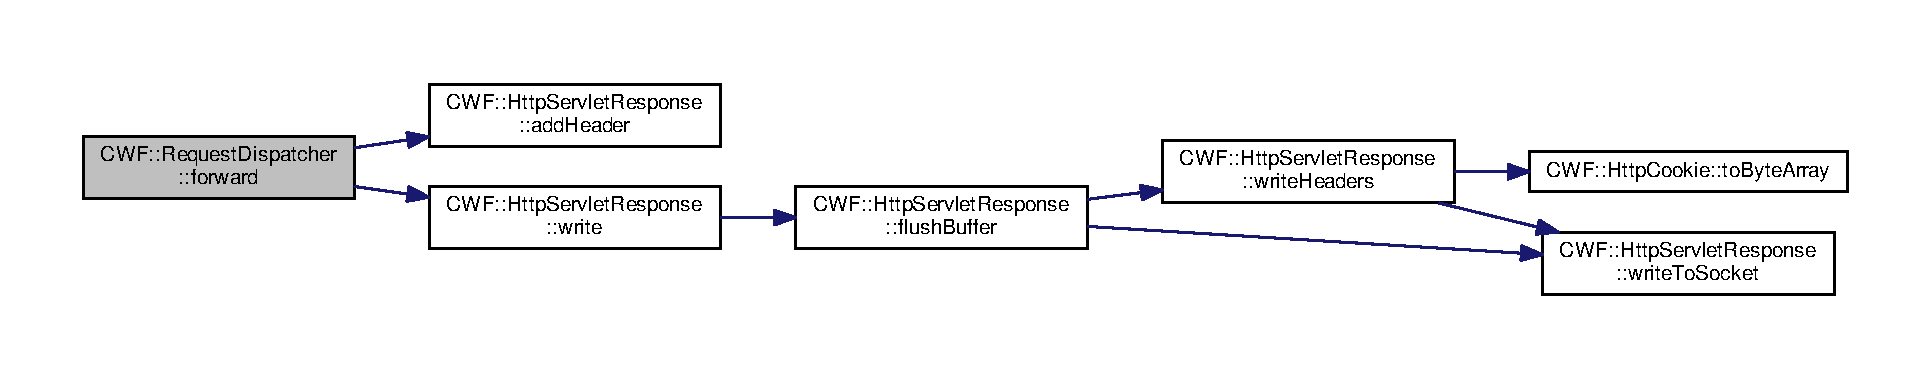
\includegraphics[width=350pt]{class_c_w_f_1_1_request_dispatcher_a075c11ff233f217196764899f9edf7d0_cgraph}
\end{center}
\end{figure}




Here is the caller graph for this function\+:
\nopagebreak
\begin{figure}[H]
\begin{center}
\leavevmode
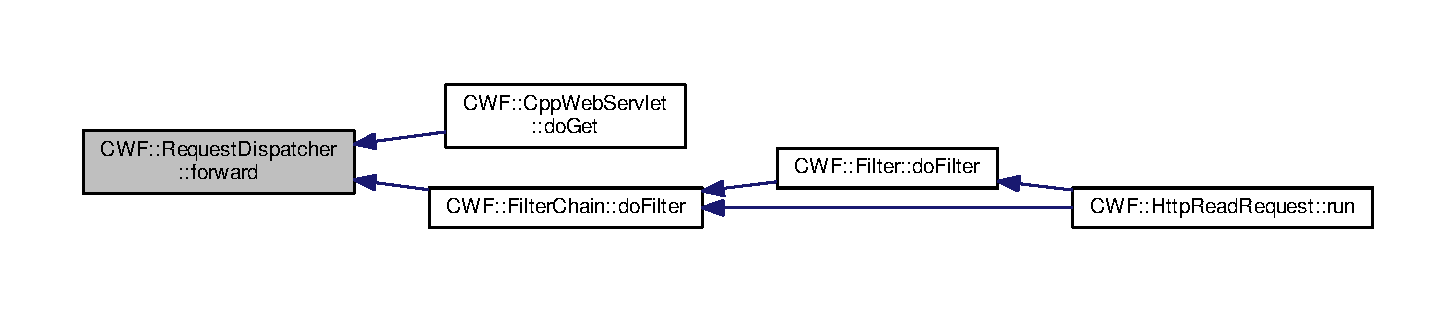
\includegraphics[width=350pt]{class_c_w_f_1_1_request_dispatcher_a075c11ff233f217196764899f9edf7d0_icgraph}
\end{center}
\end{figure}




The documentation for this class was generated from the following files\+:\begin{DoxyCompactItemize}
\item 
/home/herik/\+C\+P\+P\+Web\+Framework/\+C\+P\+P\+Web\+Framework/cwf/\hyperlink{requestdispatcher_8h}{requestdispatcher.\+h}\item 
/home/herik/\+C\+P\+P\+Web\+Framework/\+C\+P\+P\+Web\+Framework/cwf/\hyperlink{requestdispatcher_8cpp}{requestdispatcher.\+cpp}\end{DoxyCompactItemize}

\hypertarget{class_c_w_f_1_1_session_id_generator}{\section{C\+W\+F\+:\+:Session\+Id\+Generator Class Reference}
\label{class_c_w_f_1_1_session_id_generator}\index{C\+W\+F\+::\+Session\+Id\+Generator@{C\+W\+F\+::\+Session\+Id\+Generator}}
}


The \hyperlink{class_c_w_f_1_1_session_id_generator}{Session\+Id\+Generator} class is responsable to generate sessions id to the clients.  




{\ttfamily \#include $<$sessionidgenerator.\+h$>$}

\subsection*{Public Member Functions}
\begin{DoxyCompactItemize}
\item 
\hyperlink{class_c_w_f_1_1_session_id_generator_a1f7d978172454fe8b395c06b783dc355}{Session\+Id\+Generator} (const \hyperlink{class_c_w_f_1_1_http_parser}{Http\+Parser} \&http\+Parser)
\begin{DoxyCompactList}\small\item\em This constructor receives a \hyperlink{class_c_w_f_1_1_http_parser}{Http\+Parser}. \end{DoxyCompactList}\item 
Q\+Byte\+Array \hyperlink{class_c_w_f_1_1_session_id_generator_a8aada44d07a73e07c4172725519c64f9}{get\+Session\+I\+D} () const 
\begin{DoxyCompactList}\small\item\em This method process some informations of http\+Parser and generates a session id. \end{DoxyCompactList}\end{DoxyCompactItemize}


\subsection{Detailed Description}
The \hyperlink{class_c_w_f_1_1_session_id_generator}{Session\+Id\+Generator} class is responsable to generate sessions id to the clients. 

\subsection{Constructor \& Destructor Documentation}
\hypertarget{class_c_w_f_1_1_session_id_generator_a1f7d978172454fe8b395c06b783dc355}{\index{C\+W\+F\+::\+Session\+Id\+Generator@{C\+W\+F\+::\+Session\+Id\+Generator}!Session\+Id\+Generator@{Session\+Id\+Generator}}
\index{Session\+Id\+Generator@{Session\+Id\+Generator}!C\+W\+F\+::\+Session\+Id\+Generator@{C\+W\+F\+::\+Session\+Id\+Generator}}
\subsubsection[{Session\+Id\+Generator}]{\setlength{\rightskip}{0pt plus 5cm}C\+W\+F\+::\+Session\+Id\+Generator\+::\+Session\+Id\+Generator (
\begin{DoxyParamCaption}
\item[{const {\bf Http\+Parser} \&}]{http\+Parser}
\end{DoxyParamCaption}
)}}\label{class_c_w_f_1_1_session_id_generator_a1f7d978172454fe8b395c06b783dc355}


This constructor receives a \hyperlink{class_c_w_f_1_1_http_parser}{Http\+Parser}. 


\begin{DoxyParams}{Parameters}
{\em const} & \hyperlink{class_c_w_f_1_1_http_parser}{Http\+Parser} \&http\+Parser \+: Used to generate Session I\+D. \\
\hline
\end{DoxyParams}


\subsection{Member Function Documentation}
\hypertarget{class_c_w_f_1_1_session_id_generator_a8aada44d07a73e07c4172725519c64f9}{\index{C\+W\+F\+::\+Session\+Id\+Generator@{C\+W\+F\+::\+Session\+Id\+Generator}!get\+Session\+I\+D@{get\+Session\+I\+D}}
\index{get\+Session\+I\+D@{get\+Session\+I\+D}!C\+W\+F\+::\+Session\+Id\+Generator@{C\+W\+F\+::\+Session\+Id\+Generator}}
\subsubsection[{get\+Session\+I\+D}]{\setlength{\rightskip}{0pt plus 5cm}Q\+Byte\+Array C\+W\+F\+::\+Session\+Id\+Generator\+::get\+Session\+I\+D (
\begin{DoxyParamCaption}
{}
\end{DoxyParamCaption}
) const}}\label{class_c_w_f_1_1_session_id_generator_a8aada44d07a73e07c4172725519c64f9}


This method process some informations of http\+Parser and generates a session id. 

\begin{DoxyReturn}{Returns}
Q\+Byte\+Array \+: Session I\+D. 
\end{DoxyReturn}


The documentation for this class was generated from the following files\+:\begin{DoxyCompactItemize}
\item 
/home/herik/\+C\+P\+P\+Web\+Framework/\+C\+P\+P\+Web\+Framework/cwf/\hyperlink{sessionidgenerator_8h}{sessionidgenerator.\+h}\item 
/home/herik/\+C\+P\+P\+Web\+Framework/\+C\+P\+P\+Web\+Framework/cwf/\hyperlink{sessionidgenerator_8cpp}{sessionidgenerator.\+cpp}\end{DoxyCompactItemize}

\chapter{File Documentation}
\hypertarget{configuration_8cpp}{\section{/home/herik/\+C\+P\+P\+Web\+Framework/\+C\+P\+P\+Web\+Framework/cwf/configuration.cpp File Reference}
\label{configuration_8cpp}\index{/home/herik/\+C\+P\+P\+Web\+Framework/\+C\+P\+P\+Web\+Framework/cwf/configuration.\+cpp@{/home/herik/\+C\+P\+P\+Web\+Framework/\+C\+P\+P\+Web\+Framework/cwf/configuration.\+cpp}}
}
{\ttfamily \#include \char`\"{}configuration.\+h\char`\"{}}\\*
Include dependency graph for configuration.\+cpp\+:
\nopagebreak
\begin{figure}[H]
\begin{center}
\leavevmode
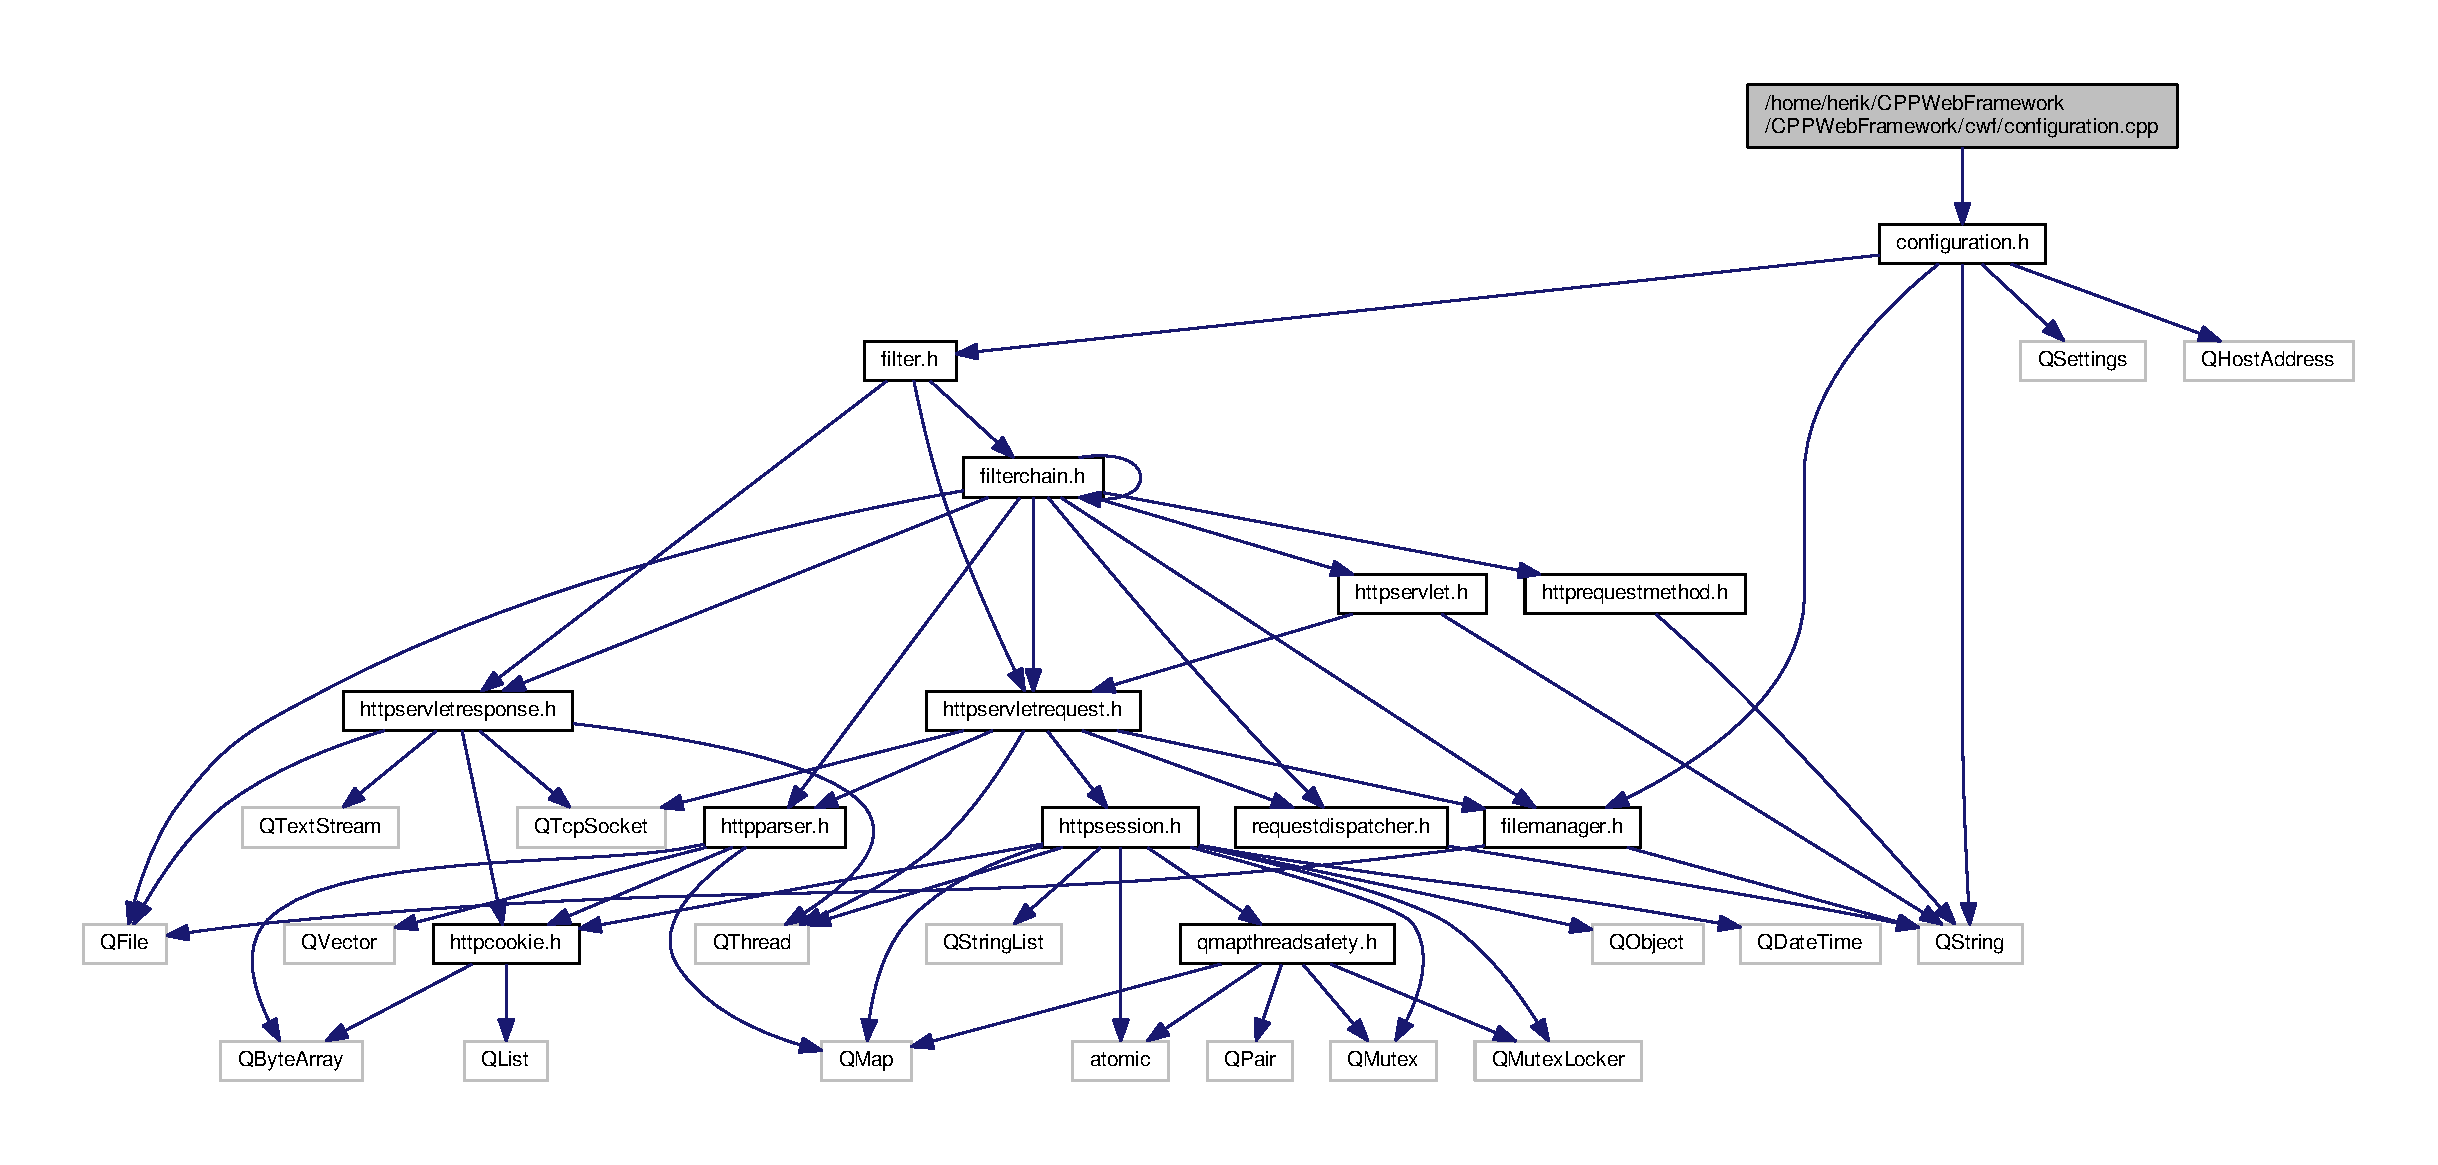
\includegraphics[width=350pt]{configuration_8cpp__incl}
\end{center}
\end{figure}
\subsection*{Namespaces}
\begin{DoxyCompactItemize}
\item 
 \hyperlink{namespace_c_w_f}{C\+W\+F}
\begin{DoxyCompactList}\small\item\em The \hyperlink{class_c_w_f_1_1_http_servlet}{Http\+Servlet} class is responsable to attend a request from a specific url. You will need to create a derived class from \hyperlink{class_c_w_f_1_1_http_servlet}{Http\+Servlet} and then, reconstruct the desired method to response a request, after this, you will need mapping the url to the new servlet that you created, you need to do it into the Configure\+Cpp\+Web\+Server using the method add\+Url\+Servlet. \end{DoxyCompactList}\end{DoxyCompactItemize}


\subsection{Detailed Description}
\begin{DoxyAuthor}{Author}
Herik Lima 
\end{DoxyAuthor}

\hypertarget{configuration_8h}{\section{/home/herik/\+C\+P\+P\+Web\+Framework/\+C\+P\+P\+Web\+Framework/cwf/configuration.h File Reference}
\label{configuration_8h}\index{/home/herik/\+C\+P\+P\+Web\+Framework/\+C\+P\+P\+Web\+Framework/cwf/configuration.\+h@{/home/herik/\+C\+P\+P\+Web\+Framework/\+C\+P\+P\+Web\+Framework/cwf/configuration.\+h}}
}
{\ttfamily \#include $<$Q\+String$>$}\\*
{\ttfamily \#include $<$Q\+Settings$>$}\\*
{\ttfamily \#include $<$Q\+Host\+Address$>$}\\*
{\ttfamily \#include \char`\"{}filter.\+h\char`\"{}}\\*
{\ttfamily \#include \char`\"{}filemanager.\+h\char`\"{}}\\*
Include dependency graph for configuration.\+h\+:\nopagebreak
\begin{figure}[H]
\begin{center}
\leavevmode
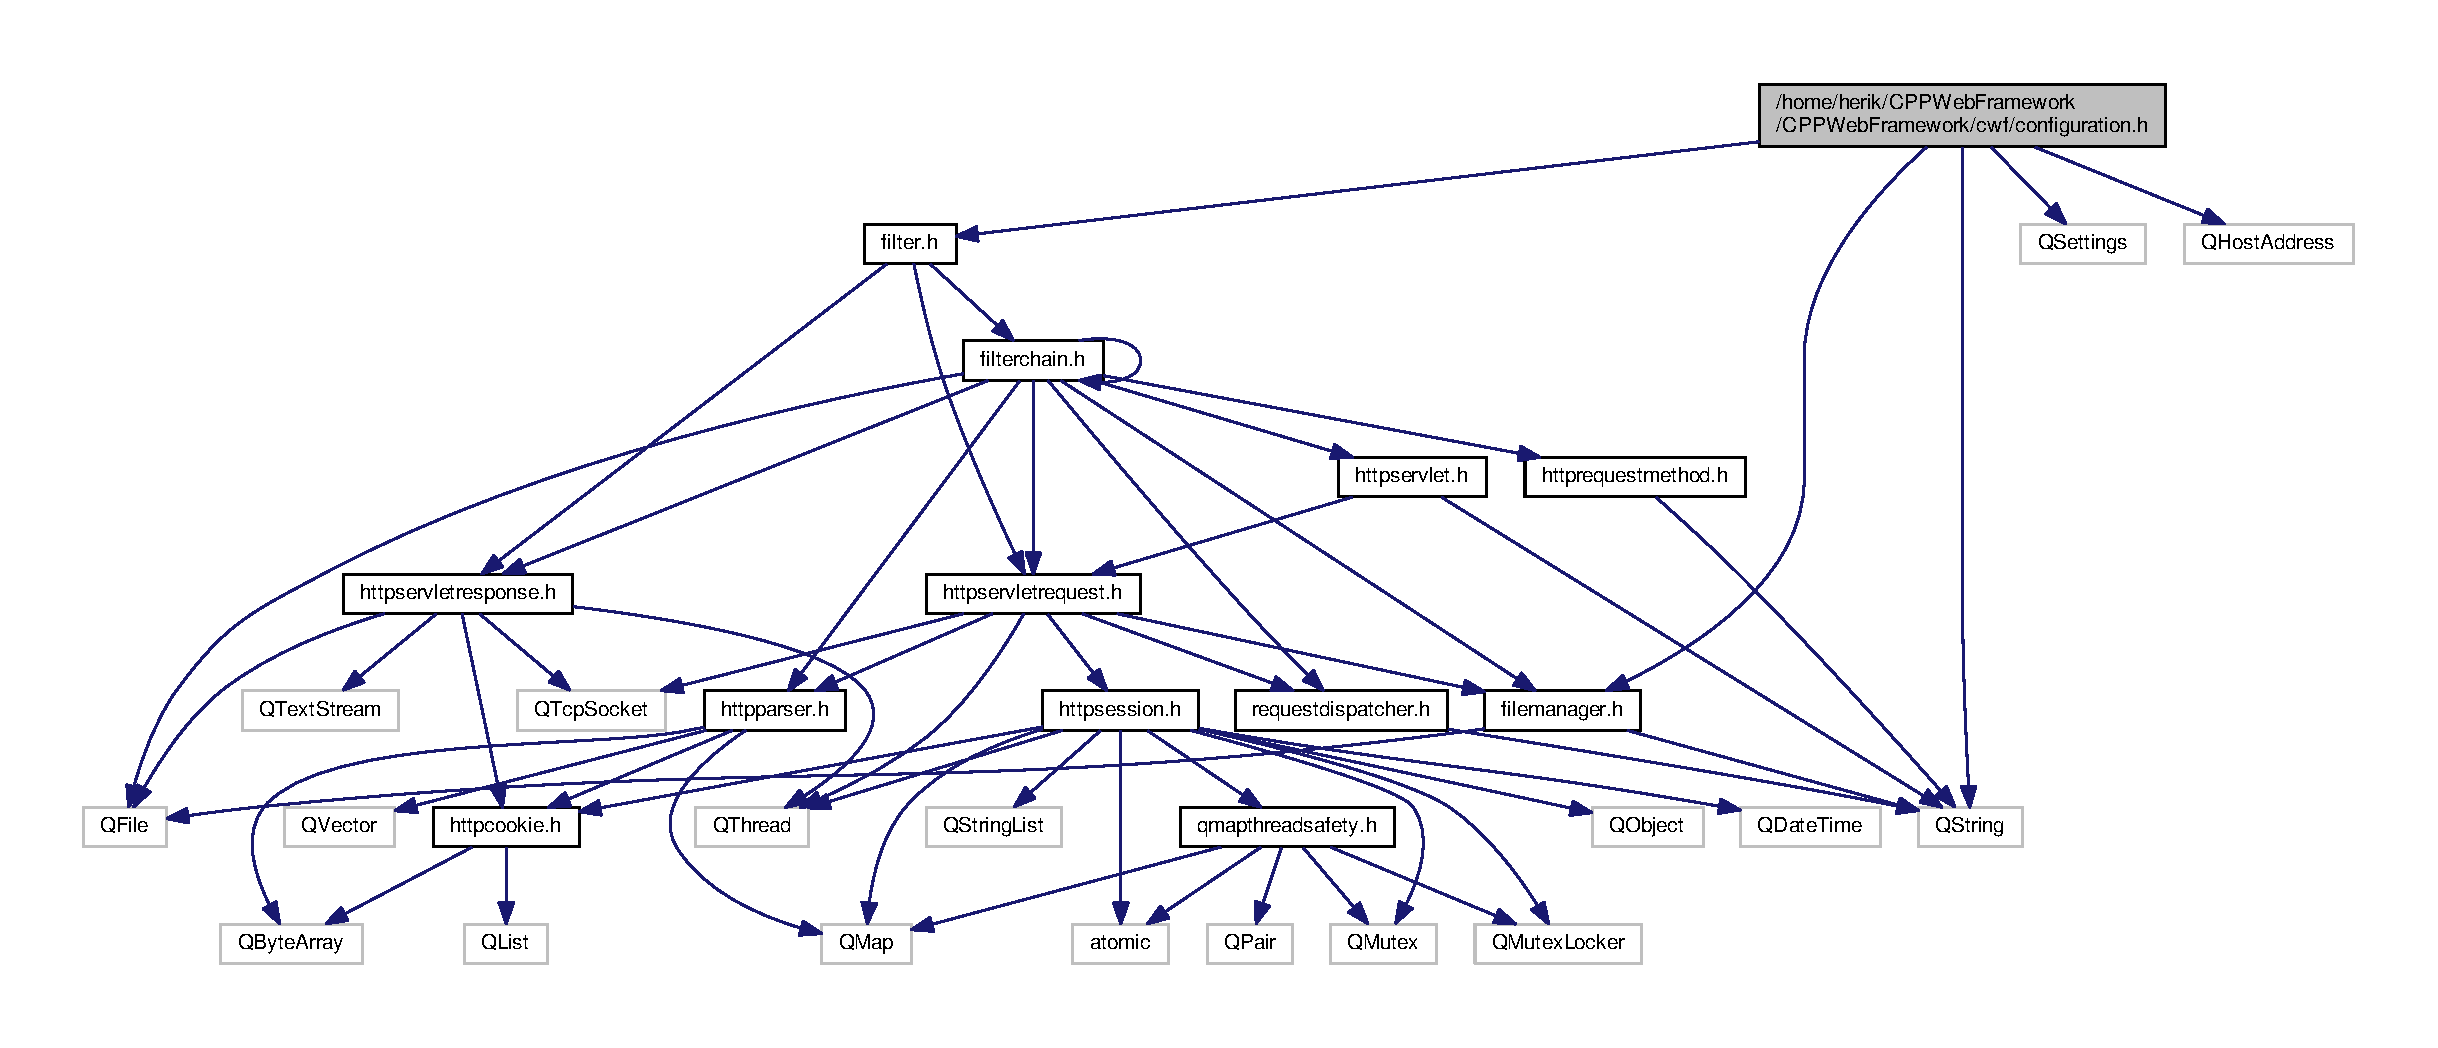
\includegraphics[width=350pt]{configuration_8h__incl}
\end{center}
\end{figure}
This graph shows which files directly or indirectly include this file\+:\nopagebreak
\begin{figure}[H]
\begin{center}
\leavevmode
\includegraphics[width=350pt]{configuration_8h__dep__incl}
\end{center}
\end{figure}
\subsection*{Classes}
\begin{DoxyCompactItemize}
\item 
class \hyperlink{class_c_w_f_1_1_configuration}{C\+W\+F\+::\+Configuration}
\begin{DoxyCompactList}\small\item\em This class is responsable to read a ini file and extract its information. \end{DoxyCompactList}\end{DoxyCompactItemize}
\subsection*{Namespaces}
\begin{DoxyCompactItemize}
\item 
 \hyperlink{namespace_c_w_f}{C\+W\+F}
\begin{DoxyCompactList}\small\item\em All classes of C++ Web Framework are contained within the namespace \hyperlink{namespace_c_w_f}{C\+W\+F}. \end{DoxyCompactList}\end{DoxyCompactItemize}


\subsection{Detailed Description}
\begin{DoxyAuthor}{Author}
Herik Lima 
\end{DoxyAuthor}

\hypertarget{cppwebapplication_8cpp}{\section{/home/herik/\+C\+P\+P\+Web\+Framework/\+C\+P\+P\+Web\+Framework/cwf/cppwebapplication.cpp File Reference}
\label{cppwebapplication_8cpp}\index{/home/herik/\+C\+P\+P\+Web\+Framework/\+C\+P\+P\+Web\+Framework/cwf/cppwebapplication.\+cpp@{/home/herik/\+C\+P\+P\+Web\+Framework/\+C\+P\+P\+Web\+Framework/cwf/cppwebapplication.\+cpp}}
}
{\ttfamily \#include \char`\"{}cppwebapplication.\+h\char`\"{}}\\*
{\ttfamily \#include \char`\"{}cppwebservlet.\+h\char`\"{}}\\*
Include dependency graph for cppwebapplication.\+cpp\+:
\nopagebreak
\begin{figure}[H]
\begin{center}
\leavevmode
\includegraphics[width=350pt]{cppwebapplication_8cpp__incl}
\end{center}
\end{figure}
\subsection*{Namespaces}
\begin{DoxyCompactItemize}
\item 
 \hyperlink{namespace_c_w_f}{C\+W\+F}
\begin{DoxyCompactList}\small\item\em All classes of C++ Web Framework are contained within the namespace \hyperlink{namespace_c_w_f}{C\+W\+F}. \end{DoxyCompactList}\end{DoxyCompactItemize}
\subsection*{Variables}
\begin{DoxyCompactItemize}
\item 
Configuration \hyperlink{namespace_c_w_f_a2f275195c5c69646f7df4e917febe552}{C\+W\+F\+::configuration}
\end{DoxyCompactItemize}


\subsection{Detailed Description}
\begin{DoxyAuthor}{Author}
Herik Lima 
\end{DoxyAuthor}

\hypertarget{cppwebapplication_8h}{\section{/home/herik/\+C\+P\+P\+Web\+Framework/\+C\+P\+P\+Web\+Framework/cwf/cppwebapplication.h File Reference}
\label{cppwebapplication_8h}\index{/home/herik/\+C\+P\+P\+Web\+Framework/\+C\+P\+P\+Web\+Framework/cwf/cppwebapplication.\+h@{/home/herik/\+C\+P\+P\+Web\+Framework/\+C\+P\+P\+Web\+Framework/cwf/cppwebapplication.\+h}}
}
{\ttfamily \#include $<$Q\+String$>$}\\*
{\ttfamily \#include $<$Q\+Core\+Application$>$}\\*
{\ttfamily \#include $<$Q\+Message\+Log\+Context$>$}\\*
{\ttfamily \#include \char`\"{}cppwebserver.\+h\char`\"{}}\\*
Include dependency graph for cppwebapplication.\+h\+:
\nopagebreak
\begin{figure}[H]
\begin{center}
\leavevmode
\includegraphics[width=350pt]{cppwebapplication_8h__incl}
\end{center}
\end{figure}
This graph shows which files directly or indirectly include this file\+:
\nopagebreak
\begin{figure}[H]
\begin{center}
\leavevmode
\includegraphics[width=310pt]{cppwebapplication_8h__dep__incl}
\end{center}
\end{figure}
\subsection*{Classes}
\begin{DoxyCompactItemize}
\item 
class \hyperlink{class_c_w_f_1_1_cpp_web_application}{C\+W\+F\+::\+Cpp\+Web\+Application}
\end{DoxyCompactItemize}
\subsection*{Namespaces}
\begin{DoxyCompactItemize}
\item 
 \hyperlink{namespace_c_w_f}{C\+W\+F}
\begin{DoxyCompactList}\small\item\em The \hyperlink{class_c_w_f_1_1_http_servlet}{Http\+Servlet} class is responsable to attend a request from a specific url. You will need to create a derived class from \hyperlink{class_c_w_f_1_1_http_servlet}{Http\+Servlet} and then, reconstruct the desired method to response a request, after this, you will need mapping the url to the new servlet that you created, you need to do it into the Configure\+Cpp\+Web\+Server using the method add\+Url\+Servlet. \end{DoxyCompactList}\end{DoxyCompactItemize}


\subsection{Detailed Description}
\begin{DoxyAuthor}{Author}
Herik Lima 
\end{DoxyAuthor}

\hypertarget{cppwebserver_8cpp}{\section{/home/herik/\+C\+P\+P\+Web\+Framework/\+C\+P\+P\+Web\+Framework/cwf/cppwebserver.cpp File Reference}
\label{cppwebserver_8cpp}\index{/home/herik/\+C\+P\+P\+Web\+Framework/\+C\+P\+P\+Web\+Framework/cwf/cppwebserver.\+cpp@{/home/herik/\+C\+P\+P\+Web\+Framework/\+C\+P\+P\+Web\+Framework/cwf/cppwebserver.\+cpp}}
}
{\ttfamily \#include \char`\"{}cppwebserver.\+h\char`\"{}}\\*
{\ttfamily \#include \char`\"{}configuration.\+h\char`\"{}}\\*
Include dependency graph for cppwebserver.\+cpp\+:
\nopagebreak
\begin{figure}[H]
\begin{center}
\leavevmode
\includegraphics[width=350pt]{cppwebserver_8cpp__incl}
\end{center}
\end{figure}
\subsection*{Namespaces}
\begin{DoxyCompactItemize}
\item 
 \hyperlink{namespace_c_w_f}{C\+W\+F}
\begin{DoxyCompactList}\small\item\em All classes of C++ Web Framework are contained within the namespace \hyperlink{namespace_c_w_f}{C\+W\+F}. \end{DoxyCompactList}\end{DoxyCompactItemize}


\subsection{Detailed Description}
\begin{DoxyAuthor}{Author}
Herik Lima 
\end{DoxyAuthor}

\hypertarget{cppwebserver_8h}{\section{/home/herik/\+C\+P\+P\+Web\+Framework/\+C\+P\+P\+Web\+Framework/cwf/cppwebserver.h File Reference}
\label{cppwebserver_8h}\index{/home/herik/\+C\+P\+P\+Web\+Framework/\+C\+P\+P\+Web\+Framework/cwf/cppwebserver.\+h@{/home/herik/\+C\+P\+P\+Web\+Framework/\+C\+P\+P\+Web\+Framework/cwf/cppwebserver.\+h}}
}
{\ttfamily \#include $<$Q\+Tcp\+Server$>$}\\*
{\ttfamily \#include $<$Q\+Ssl\+Key$>$}\\*
{\ttfamily \#include $<$Q\+Ssl\+Certificate$>$}\\*
{\ttfamily \#include $<$Q\+Http\+Multi\+Part$>$}\\*
{\ttfamily \#include $<$Q\+Mutex$>$}\\*
{\ttfamily \#include $<$Q\+Thread\+Pool$>$}\\*
{\ttfamily \#include $<$Q\+Timer$>$}\\*
{\ttfamily \#include $<$atomic$>$}\\*
{\ttfamily \#include \char`\"{}qmapthreadsafety.\+h\char`\"{}}\\*
{\ttfamily \#include \char`\"{}httpreadrequest.\+h\char`\"{}}\\*
{\ttfamily \#include \char`\"{}httpservlet.\+h\char`\"{}}\\*
{\ttfamily \#include \char`\"{}httpsession.\+h\char`\"{}}\\*
{\ttfamily \#include \char`\"{}filter.\+h\char`\"{}}\\*
{\ttfamily \#include \char`\"{}httpservletrequest.\+h\char`\"{}}\\*
{\ttfamily \#include \char`\"{}httpservletresponse.\+h\char`\"{}}\\*
{\ttfamily \#include \char`\"{}configuration.\+h\char`\"{}}\\*
Include dependency graph for cppwebserver.\+h\+:\nopagebreak
\begin{figure}[H]
\begin{center}
\leavevmode
\includegraphics[width=350pt]{cppwebserver_8h__incl}
\end{center}
\end{figure}
This graph shows which files directly or indirectly include this file\+:\nopagebreak
\begin{figure}[H]
\begin{center}
\leavevmode
\includegraphics[width=350pt]{cppwebserver_8h__dep__incl}
\end{center}
\end{figure}
\subsection*{Classes}
\begin{DoxyCompactItemize}
\item 
class \hyperlink{class_c_w_f_1_1_cpp_web_server}{C\+W\+F\+::\+Cpp\+Web\+Server}
\begin{DoxyCompactList}\small\item\em The \hyperlink{class_c_w_f_1_1_cpp_web_server}{Cpp\+Web\+Server} class is a H\+T\+T\+P server, responsable to receive and dispatch the requisitions. \end{DoxyCompactList}\end{DoxyCompactItemize}
\subsection*{Namespaces}
\begin{DoxyCompactItemize}
\item 
 \hyperlink{namespace_c_w_f}{C\+W\+F}
\begin{DoxyCompactList}\small\item\em All classes of C++ Web Framework are contained within the namespace \hyperlink{namespace_c_w_f}{C\+W\+F}. \end{DoxyCompactList}\end{DoxyCompactItemize}


\subsection{Detailed Description}
\begin{DoxyAuthor}{Author}
Herik Lima 
\end{DoxyAuthor}

\hypertarget{cppwebservlet_8cpp}{\section{/home/herik/\+C\+P\+P\+Web\+Framework/\+C\+P\+P\+Web\+Framework/cwf/cppwebservlet.cpp File Reference}
\label{cppwebservlet_8cpp}\index{/home/herik/\+C\+P\+P\+Web\+Framework/\+C\+P\+P\+Web\+Framework/cwf/cppwebservlet.\+cpp@{/home/herik/\+C\+P\+P\+Web\+Framework/\+C\+P\+P\+Web\+Framework/cwf/cppwebservlet.\+cpp}}
}
{\ttfamily \#include \char`\"{}cppwebservlet.\+h\char`\"{}}\\*
Include dependency graph for cppwebservlet.\+cpp\+:
\nopagebreak
\begin{figure}[H]
\begin{center}
\leavevmode
\includegraphics[width=350pt]{cppwebservlet_8cpp__incl}
\end{center}
\end{figure}
\subsection*{Namespaces}
\begin{DoxyCompactItemize}
\item 
 \hyperlink{namespace_c_w_f}{C\+W\+F}
\begin{DoxyCompactList}\small\item\em All classes of C++ Web Framework are contained within the namespace \hyperlink{namespace_c_w_f}{C\+W\+F}. \end{DoxyCompactList}\end{DoxyCompactItemize}


\subsection{Detailed Description}
\begin{DoxyAuthor}{Author}
Herik Lima 
\end{DoxyAuthor}

\hypertarget{cppwebservlet_8h}{\section{/home/herik/\+C\+P\+P\+Web\+Framework/\+C\+P\+P\+Web\+Framework/cwf/cppwebservlet.h File Reference}
\label{cppwebservlet_8h}\index{/home/herik/\+C\+P\+P\+Web\+Framework/\+C\+P\+P\+Web\+Framework/cwf/cppwebservlet.\+h@{/home/herik/\+C\+P\+P\+Web\+Framework/\+C\+P\+P\+Web\+Framework/cwf/cppwebservlet.\+h}}
}
{\ttfamily \#include \char`\"{}httpservlet.\+h\char`\"{}}\\*
{\ttfamily \#include \char`\"{}httpservletrequest.\+h\char`\"{}}\\*
{\ttfamily \#include \char`\"{}httpservletresponse.\+h\char`\"{}}\\*
Include dependency graph for cppwebservlet.\+h\+:
\nopagebreak
\begin{figure}[H]
\begin{center}
\leavevmode
\includegraphics[width=350pt]{cppwebservlet_8h__incl}
\end{center}
\end{figure}
This graph shows which files directly or indirectly include this file\+:
\nopagebreak
\begin{figure}[H]
\begin{center}
\leavevmode
\includegraphics[width=350pt]{cppwebservlet_8h__dep__incl}
\end{center}
\end{figure}
\subsection*{Classes}
\begin{DoxyCompactItemize}
\item 
class \hyperlink{class_c_w_f_1_1_cpp_web_servlet}{C\+W\+F\+::\+Cpp\+Web\+Servlet}
\begin{DoxyCompactList}\small\item\em This class is responsible for displaying the standard pages of C++ Web Framework\+: index, examples, documentation, ssl and authors. \end{DoxyCompactList}\end{DoxyCompactItemize}
\subsection*{Namespaces}
\begin{DoxyCompactItemize}
\item 
 \hyperlink{namespace_c_w_f}{C\+W\+F}
\begin{DoxyCompactList}\small\item\em All classes of C++ Web Framework are contained within the namespace \hyperlink{namespace_c_w_f}{C\+W\+F}. \end{DoxyCompactList}\end{DoxyCompactItemize}


\subsection{Detailed Description}
\begin{DoxyAuthor}{Author}
Herik Lima 
\end{DoxyAuthor}

\hypertarget{cstlcompiler_8cpp}{\section{/home/herik/\+C\+P\+P\+Web\+Framework/\+C\+P\+P\+Web\+Framework/cwf/cstlcompiler.cpp File Reference}
\label{cstlcompiler_8cpp}\index{/home/herik/\+C\+P\+P\+Web\+Framework/\+C\+P\+P\+Web\+Framework/cwf/cstlcompiler.\+cpp@{/home/herik/\+C\+P\+P\+Web\+Framework/\+C\+P\+P\+Web\+Framework/cwf/cstlcompiler.\+cpp}}
}
{\ttfamily \#include \char`\"{}cstlcompiler.\+h\char`\"{}}\\*
{\ttfamily \#include \char`\"{}cstlcompilerattributes.\+h\char`\"{}}\\*
{\ttfamily \#include \char`\"{}cstlcompilerfor.\+h\char`\"{}}\\*
{\ttfamily \#include \char`\"{}cstlcompilerobject.\+h\char`\"{}}\\*
{\ttfamily \#include \char`\"{}cstlcompilerif.\+h\char`\"{}}\\*
Include dependency graph for cstlcompiler.\+cpp\+:
\nopagebreak
\begin{figure}[H]
\begin{center}
\leavevmode
\includegraphics[width=350pt]{cstlcompiler_8cpp__incl}
\end{center}
\end{figure}
\subsection*{Namespaces}
\begin{DoxyCompactItemize}
\item 
 \hyperlink{namespace_c_w_f}{C\+W\+F}
\begin{DoxyCompactList}\small\item\em All classes of C++ Web Framework are contained within the namespace \hyperlink{namespace_c_w_f}{C\+W\+F}. \end{DoxyCompactList}\end{DoxyCompactItemize}


\subsection{Detailed Description}
\begin{DoxyAuthor}{Author}
Herik Lima 
\end{DoxyAuthor}

\hypertarget{cstlcompiler_8h}{\section{/home/herik/\+C\+P\+P\+Web\+Framework/\+C\+P\+P\+Web\+Framework/cwf/cstlcompiler.h File Reference}
\label{cstlcompiler_8h}\index{/home/herik/\+C\+P\+P\+Web\+Framework/\+C\+P\+P\+Web\+Framework/cwf/cstlcompiler.\+h@{/home/herik/\+C\+P\+P\+Web\+Framework/\+C\+P\+P\+Web\+Framework/cwf/cstlcompiler.\+h}}
}
{\ttfamily \#include $<$Q\+Map$>$}\\*
{\ttfamily \#include $<$Q\+File$>$}\\*
{\ttfamily \#include $<$Q\+String$>$}\\*
{\ttfamily \#include $<$Q\+Xml\+Stream\+Reader$>$}\\*
{\ttfamily \#include $<$Q\+Xml\+Stream\+Writer$>$}\\*
{\ttfamily \#include $<$Q\+String\+List$>$}\\*
{\ttfamily \#include $<$Q\+Meta\+Object$>$}\\*
{\ttfamily \#include $<$Q\+Meta\+Method$>$}\\*
{\ttfamily \#include $<$qdebug.\+h$>$}\\*
{\ttfamily \#include $<$vector$>$}\\*
{\ttfamily \#include \char`\"{}properties.\+h\char`\"{}}\\*
{\ttfamily \#include \char`\"{}forattributes.\+h\char`\"{}}\\*
{\ttfamily \#include \char`\"{}qlistobject.\+h\char`\"{}}\\*
{\ttfamily \#include \char`\"{}ifattributes.\+h\char`\"{}}\\*
Include dependency graph for cstlcompiler.\+h\+:
\nopagebreak
\begin{figure}[H]
\begin{center}
\leavevmode
\includegraphics[width=350pt]{cstlcompiler_8h__incl}
\end{center}
\end{figure}
This graph shows which files directly or indirectly include this file\+:
\nopagebreak
\begin{figure}[H]
\begin{center}
\leavevmode
\includegraphics[width=350pt]{cstlcompiler_8h__dep__incl}
\end{center}
\end{figure}
\subsection*{Classes}
\begin{DoxyCompactItemize}
\item 
class \hyperlink{class_c_w_f_1_1_c_s_t_l_compiler}{C\+W\+F\+::\+C\+S\+T\+L\+Compiler}
\begin{DoxyCompactList}\small\item\em This class compiles xhtml pages with C\+S\+T\+L (C++ Server Pages Standard Tags Library). \end{DoxyCompactList}\end{DoxyCompactItemize}
\subsection*{Namespaces}
\begin{DoxyCompactItemize}
\item 
 \hyperlink{namespace_c_w_f}{C\+W\+F}
\begin{DoxyCompactList}\small\item\em All classes of C++ Web Framework are contained within the namespace \hyperlink{namespace_c_w_f}{C\+W\+F}. \end{DoxyCompactList}\end{DoxyCompactItemize}


\subsection{Detailed Description}
\begin{DoxyAuthor}{Author}
Herik Lima 
\end{DoxyAuthor}

\hypertarget{cstlcompilerattributes_8cpp}{\section{/home/herik/\+C\+P\+P\+Web\+Framework/\+C\+P\+P\+Web\+Framework/cwf/cstlcompilerattributes.cpp File Reference}
\label{cstlcompilerattributes_8cpp}\index{/home/herik/\+C\+P\+P\+Web\+Framework/\+C\+P\+P\+Web\+Framework/cwf/cstlcompilerattributes.\+cpp@{/home/herik/\+C\+P\+P\+Web\+Framework/\+C\+P\+P\+Web\+Framework/cwf/cstlcompilerattributes.\+cpp}}
}
{\ttfamily \#include \char`\"{}cstlcompilerattributes.\+h\char`\"{}}\\*
{\ttfamily \#include $<$Q\+Variant$>$}\\*
{\ttfamily \#include $<$cwf/metaclassparser.\+h$>$}\\*
Include dependency graph for cstlcompilerattributes.\+cpp\+:\nopagebreak
\begin{figure}[H]
\begin{center}
\leavevmode
\includegraphics[width=350pt]{cstlcompilerattributes_8cpp__incl}
\end{center}
\end{figure}
\subsection*{Namespaces}
\begin{DoxyCompactItemize}
\item 
 \hyperlink{namespace_c_w_f}{C\+W\+F}
\begin{DoxyCompactList}\small\item\em All classes of C++ Web Framework are contained within the namespace \hyperlink{namespace_c_w_f}{C\+W\+F}. \end{DoxyCompactList}\end{DoxyCompactItemize}


\subsection{Detailed Description}
\begin{DoxyAuthor}{Author}
Herik Lima 
\end{DoxyAuthor}

\hypertarget{cstlcompilerattributes_8h}{\section{/home/herik/\+C\+P\+P\+Web\+Framework/\+C\+P\+P\+Web\+Framework/cwf/cstlcompilerattributes.h File Reference}
\label{cstlcompilerattributes_8h}\index{/home/herik/\+C\+P\+P\+Web\+Framework/\+C\+P\+P\+Web\+Framework/cwf/cstlcompilerattributes.\+h@{/home/herik/\+C\+P\+P\+Web\+Framework/\+C\+P\+P\+Web\+Framework/cwf/cstlcompilerattributes.\+h}}
}
{\ttfamily \#include $<$Q\+Map$>$}\\*
{\ttfamily \#include $<$Q\+String$>$}\\*
{\ttfamily \#include $<$Q\+Object$>$}\\*
{\ttfamily \#include $<$Q\+Xml\+Stream\+Attributes$>$}\\*
{\ttfamily \#include \char`\"{}properties.\+h\char`\"{}}\\*
Include dependency graph for cstlcompilerattributes.\+h\+:\nopagebreak
\begin{figure}[H]
\begin{center}
\leavevmode
\includegraphics[width=350pt]{cstlcompilerattributes_8h__incl}
\end{center}
\end{figure}
This graph shows which files directly or indirectly include this file\+:\nopagebreak
\begin{figure}[H]
\begin{center}
\leavevmode
\includegraphics[width=350pt]{cstlcompilerattributes_8h__dep__incl}
\end{center}
\end{figure}
\subsection*{Classes}
\begin{DoxyCompactItemize}
\item 
class \hyperlink{class_c_w_f_1_1_c_s_t_l_compiler_attributes}{C\+W\+F\+::\+C\+S\+T\+L\+Compiler\+Attributes}
\begin{DoxyCompactList}\small\item\em This class search for expressions \#\{obj.\+get\} and compiles it. \end{DoxyCompactList}\end{DoxyCompactItemize}
\subsection*{Namespaces}
\begin{DoxyCompactItemize}
\item 
 \hyperlink{namespace_c_w_f}{C\+W\+F}
\begin{DoxyCompactList}\small\item\em All classes of C++ Web Framework are contained within the namespace \hyperlink{namespace_c_w_f}{C\+W\+F}. \end{DoxyCompactList}\end{DoxyCompactItemize}


\subsection{Detailed Description}
\begin{DoxyAuthor}{Author}
Herik Lima 
\end{DoxyAuthor}

\hypertarget{cstlcompilerfor_8cpp}{\section{/home/herik/\+C\+P\+P\+Web\+Framework/\+C\+P\+P\+Web\+Framework/cwf/cstlcompilerfor.cpp File Reference}
\label{cstlcompilerfor_8cpp}\index{/home/herik/\+C\+P\+P\+Web\+Framework/\+C\+P\+P\+Web\+Framework/cwf/cstlcompilerfor.\+cpp@{/home/herik/\+C\+P\+P\+Web\+Framework/\+C\+P\+P\+Web\+Framework/cwf/cstlcompilerfor.\+cpp}}
}
{\ttfamily \#include \char`\"{}cstlcompilerfor.\+h\char`\"{}}\\*
Include dependency graph for cstlcompilerfor.\+cpp\+:
\nopagebreak
\begin{figure}[H]
\begin{center}
\leavevmode
\includegraphics[width=294pt]{cstlcompilerfor_8cpp__incl}
\end{center}
\end{figure}
\subsection*{Namespaces}
\begin{DoxyCompactItemize}
\item 
 \hyperlink{namespace_c_w_f}{C\+W\+F}
\begin{DoxyCompactList}\small\item\em All classes of C++ Web Framework are contained within the namespace \hyperlink{namespace_c_w_f}{C\+W\+F}. \end{DoxyCompactList}\end{DoxyCompactItemize}


\subsection{Detailed Description}
\begin{DoxyAuthor}{Author}
Herik Lima 
\end{DoxyAuthor}

\hypertarget{cstlcompilerfor_8h}{\section{/home/herik/\+C\+P\+P\+Web\+Framework/\+C\+P\+P\+Web\+Framework/cwf/cstlcompilerfor.h File Reference}
\label{cstlcompilerfor_8h}\index{/home/herik/\+C\+P\+P\+Web\+Framework/\+C\+P\+P\+Web\+Framework/cwf/cstlcompilerfor.\+h@{/home/herik/\+C\+P\+P\+Web\+Framework/\+C\+P\+P\+Web\+Framework/cwf/cstlcompilerfor.\+h}}
}
{\ttfamily \#include $<$Q\+Map$>$}\\*
{\ttfamily \#include $<$Q\+Xml\+Stream\+Attributes$>$}\\*
Include dependency graph for cstlcompilerfor.\+h\+:
\nopagebreak
\begin{figure}[H]
\begin{center}
\leavevmode
\includegraphics[width=288pt]{cstlcompilerfor_8h__incl}
\end{center}
\end{figure}
This graph shows which files directly or indirectly include this file\+:
\nopagebreak
\begin{figure}[H]
\begin{center}
\leavevmode
\includegraphics[width=350pt]{cstlcompilerfor_8h__dep__incl}
\end{center}
\end{figure}
\subsection*{Classes}
\begin{DoxyCompactItemize}
\item 
class \hyperlink{class_c_w_f_1_1_c_s_t_l_compiler_for}{C\+W\+F\+::\+C\+S\+T\+L\+Compiler\+For}
\end{DoxyCompactItemize}
\subsection*{Namespaces}
\begin{DoxyCompactItemize}
\item 
 \hyperlink{namespace_c_w_f}{C\+W\+F}
\begin{DoxyCompactList}\small\item\em All classes of C++ Web Framework are contained within the namespace \hyperlink{namespace_c_w_f}{C\+W\+F}. \end{DoxyCompactList}\end{DoxyCompactItemize}


\subsection{Detailed Description}
\begin{DoxyAuthor}{Author}
Herik Lima 
\end{DoxyAuthor}

\hypertarget{cstlcompilerif_8cpp}{\section{/home/herik/\+C\+P\+P\+Web\+Framework/\+C\+P\+P\+Web\+Framework/cwf/cstlcompilerif.cpp File Reference}
\label{cstlcompilerif_8cpp}\index{/home/herik/\+C\+P\+P\+Web\+Framework/\+C\+P\+P\+Web\+Framework/cwf/cstlcompilerif.\+cpp@{/home/herik/\+C\+P\+P\+Web\+Framework/\+C\+P\+P\+Web\+Framework/cwf/cstlcompilerif.\+cpp}}
}
{\ttfamily \#include \char`\"{}cstlcompilerif.\+h\char`\"{}}\\*
Include dependency graph for cstlcompilerif.\+cpp\+:
\nopagebreak
\begin{figure}[H]
\begin{center}
\leavevmode
\includegraphics[width=291pt]{cstlcompilerif_8cpp__incl}
\end{center}
\end{figure}
\subsection*{Namespaces}
\begin{DoxyCompactItemize}
\item 
 \hyperlink{namespace_c_w_f}{C\+W\+F}
\begin{DoxyCompactList}\small\item\em All classes of C++ Web Framework are contained within the namespace \hyperlink{namespace_c_w_f}{C\+W\+F}. \end{DoxyCompactList}\end{DoxyCompactItemize}


\subsection{Detailed Description}
\begin{DoxyAuthor}{Author}
Herik Lima 
\end{DoxyAuthor}

\hypertarget{cstlcompilerif_8h}{\section{/home/herik/\+C\+P\+P\+Web\+Framework/\+C\+P\+P\+Web\+Framework/cwf/cstlcompilerif.h File Reference}
\label{cstlcompilerif_8h}\index{/home/herik/\+C\+P\+P\+Web\+Framework/\+C\+P\+P\+Web\+Framework/cwf/cstlcompilerif.\+h@{/home/herik/\+C\+P\+P\+Web\+Framework/\+C\+P\+P\+Web\+Framework/cwf/cstlcompilerif.\+h}}
}
{\ttfamily \#include $<$Q\+Map$>$}\\*
{\ttfamily \#include $<$Q\+Xml\+Stream\+Attributes$>$}\\*
Include dependency graph for cstlcompilerif.\+h\+:
\nopagebreak
\begin{figure}[H]
\begin{center}
\leavevmode
\includegraphics[width=285pt]{cstlcompilerif_8h__incl}
\end{center}
\end{figure}
This graph shows which files directly or indirectly include this file\+:
\nopagebreak
\begin{figure}[H]
\begin{center}
\leavevmode
\includegraphics[width=350pt]{cstlcompilerif_8h__dep__incl}
\end{center}
\end{figure}
\subsection*{Classes}
\begin{DoxyCompactItemize}
\item 
class \hyperlink{class_c_w_f_1_1_c_s_t_l_compiler_if}{C\+W\+F\+::\+C\+S\+T\+L\+Compiler\+If}
\end{DoxyCompactItemize}
\subsection*{Namespaces}
\begin{DoxyCompactItemize}
\item 
 \hyperlink{namespace_c_w_f}{C\+W\+F}
\begin{DoxyCompactList}\small\item\em All classes of C++ Web Framework are contained within the namespace \hyperlink{namespace_c_w_f}{C\+W\+F}. \end{DoxyCompactList}\end{DoxyCompactItemize}


\subsection{Detailed Description}
\begin{DoxyAuthor}{Author}
Herik Lima 
\end{DoxyAuthor}

\hypertarget{cstlcompilerobject_8cpp}{\section{/home/herik/\+C\+P\+P\+Web\+Framework/\+C\+P\+P\+Web\+Framework/cwf/cstlcompilerobject.cpp File Reference}
\label{cstlcompilerobject_8cpp}\index{/home/herik/\+C\+P\+P\+Web\+Framework/\+C\+P\+P\+Web\+Framework/cwf/cstlcompilerobject.\+cpp@{/home/herik/\+C\+P\+P\+Web\+Framework/\+C\+P\+P\+Web\+Framework/cwf/cstlcompilerobject.\+cpp}}
}
{\ttfamily \#include \char`\"{}cstlcompilerobject.\+h\char`\"{}}\\*
Include dependency graph for cstlcompilerobject.\+cpp\+:
\nopagebreak
\begin{figure}[H]
\begin{center}
\leavevmode
\includegraphics[width=309pt]{cstlcompilerobject_8cpp__incl}
\end{center}
\end{figure}
\subsection*{Namespaces}
\begin{DoxyCompactItemize}
\item 
 \hyperlink{namespace_c_w_f}{C\+W\+F}
\begin{DoxyCompactList}\small\item\em All classes of C++ Web Framework are contained within the namespace \hyperlink{namespace_c_w_f}{C\+W\+F}. \end{DoxyCompactList}\end{DoxyCompactItemize}

\hypertarget{cstlcompilerobject_8h}{\section{/home/herik/\+C\+P\+P\+Web\+Framework/\+C\+P\+P\+Web\+Framework/cwf/cstlcompilerobject.h File Reference}
\label{cstlcompilerobject_8h}\index{/home/herik/\+C\+P\+P\+Web\+Framework/\+C\+P\+P\+Web\+Framework/cwf/cstlcompilerobject.\+h@{/home/herik/\+C\+P\+P\+Web\+Framework/\+C\+P\+P\+Web\+Framework/cwf/cstlcompilerobject.\+h}}
}
{\ttfamily \#include $<$Q\+Object$>$}\\*
Include dependency graph for cstlcompilerobject.\+h\+:
\nopagebreak
\begin{figure}[H]
\begin{center}
\leavevmode
\includegraphics[width=298pt]{cstlcompilerobject_8h__incl}
\end{center}
\end{figure}
This graph shows which files directly or indirectly include this file\+:
\nopagebreak
\begin{figure}[H]
\begin{center}
\leavevmode
\includegraphics[width=350pt]{cstlcompilerobject_8h__dep__incl}
\end{center}
\end{figure}
\subsection*{Classes}
\begin{DoxyCompactItemize}
\item 
class \hyperlink{class_c_w_f_1_1_c_s_t_l_compiler_object}{C\+W\+F\+::\+C\+S\+T\+L\+Compiler\+Object}
\end{DoxyCompactItemize}
\subsection*{Namespaces}
\begin{DoxyCompactItemize}
\item 
 \hyperlink{namespace_c_w_f}{C\+W\+F}
\begin{DoxyCompactList}\small\item\em The \hyperlink{class_c_w_f_1_1_http_servlet}{Http\+Servlet} class is responsable to attend a request from a specific url. You will need to create a derived class from \hyperlink{class_c_w_f_1_1_http_servlet}{Http\+Servlet} and then, reconstruct the desired method to response a request, after this, you will need mapping the url to the new servlet that you created, you need to do it into the Configure\+Cpp\+Web\+Server using the method add\+Url\+Servlet. \end{DoxyCompactList}\end{DoxyCompactItemize}


\subsection{Detailed Description}
\begin{DoxyAuthor}{Author}
Herik Lima 
\end{DoxyAuthor}

\hypertarget{filemanager_8cpp}{\section{/home/herik/\+C\+P\+P\+Web\+Framework/\+C\+P\+P\+Web\+Framework/cwf/filemanager.cpp File Reference}
\label{filemanager_8cpp}\index{/home/herik/\+C\+P\+P\+Web\+Framework/\+C\+P\+P\+Web\+Framework/cwf/filemanager.\+cpp@{/home/herik/\+C\+P\+P\+Web\+Framework/\+C\+P\+P\+Web\+Framework/cwf/filemanager.\+cpp}}
}
{\ttfamily \#include \char`\"{}filemanager.\+h\char`\"{}}\\*
Include dependency graph for filemanager.\+cpp\+:
\nopagebreak
\begin{figure}[H]
\begin{center}
\leavevmode
\includegraphics[width=280pt]{filemanager_8cpp__incl}
\end{center}
\end{figure}
\subsection*{Namespaces}
\begin{DoxyCompactItemize}
\item 
 \hyperlink{namespace_c_w_f}{C\+W\+F}
\begin{DoxyCompactList}\small\item\em All classes of C++ Web Framework are contained within the namespace \hyperlink{namespace_c_w_f}{C\+W\+F}. \end{DoxyCompactList}\end{DoxyCompactItemize}


\subsection{Detailed Description}
\begin{DoxyAuthor}{Author}
Herik Lima 
\end{DoxyAuthor}

\hypertarget{filemanager_8h}{\section{/home/herik/\+C\+P\+P\+Web\+Framework/\+C\+P\+P\+Web\+Framework/cwf/filemanager.h File Reference}
\label{filemanager_8h}\index{/home/herik/\+C\+P\+P\+Web\+Framework/\+C\+P\+P\+Web\+Framework/cwf/filemanager.\+h@{/home/herik/\+C\+P\+P\+Web\+Framework/\+C\+P\+P\+Web\+Framework/cwf/filemanager.\+h}}
}
{\ttfamily \#include $<$Q\+String$>$}\\*
{\ttfamily \#include $<$Q\+File$>$}\\*
Include dependency graph for filemanager.\+h\+:
\nopagebreak
\begin{figure}[H]
\begin{center}
\leavevmode
\includegraphics[width=270pt]{filemanager_8h__incl}
\end{center}
\end{figure}
This graph shows which files directly or indirectly include this file\+:
\nopagebreak
\begin{figure}[H]
\begin{center}
\leavevmode
\includegraphics[width=350pt]{filemanager_8h__dep__incl}
\end{center}
\end{figure}
\subsection*{Classes}
\begin{DoxyCompactItemize}
\item 
class \hyperlink{class_c_w_f_1_1_file_manager}{C\+W\+F\+::\+File\+Manager}
\begin{DoxyCompactList}\small\item\em The \hyperlink{class_c_w_f_1_1_file_manager}{File\+Manager} class can manage file's name. \end{DoxyCompactList}\end{DoxyCompactItemize}
\subsection*{Namespaces}
\begin{DoxyCompactItemize}
\item 
 \hyperlink{namespace_c_w_f}{C\+W\+F}
\begin{DoxyCompactList}\small\item\em All classes of C++ Web Framework are contained within the namespace \hyperlink{namespace_c_w_f}{C\+W\+F}. \end{DoxyCompactList}\end{DoxyCompactItemize}


\subsection{Detailed Description}
\begin{DoxyAuthor}{Author}
Herik Lima 
\end{DoxyAuthor}

\hypertarget{filter_8cpp}{\section{/home/herik/\+C\+P\+P\+Web\+Framework/\+C\+P\+P\+Web\+Framework/cwf/filter.cpp File Reference}
\label{filter_8cpp}\index{/home/herik/\+C\+P\+P\+Web\+Framework/\+C\+P\+P\+Web\+Framework/cwf/filter.\+cpp@{/home/herik/\+C\+P\+P\+Web\+Framework/\+C\+P\+P\+Web\+Framework/cwf/filter.\+cpp}}
}
{\ttfamily \#include \char`\"{}filter.\+h\char`\"{}}\\*
Include dependency graph for filter.\+cpp\+:\nopagebreak
\begin{figure}[H]
\begin{center}
\leavevmode
\includegraphics[width=350pt]{filter_8cpp__incl}
\end{center}
\end{figure}
\subsection*{Namespaces}
\begin{DoxyCompactItemize}
\item 
 \hyperlink{namespace_c_w_f}{C\+W\+F}
\begin{DoxyCompactList}\small\item\em All classes of C++ Web Framework are contained within the namespace \hyperlink{namespace_c_w_f}{C\+W\+F}. \end{DoxyCompactList}\end{DoxyCompactItemize}


\subsection{Detailed Description}
\begin{DoxyAuthor}{Author}
Herik Lima 
\end{DoxyAuthor}

\hypertarget{filter_8h}{\section{/home/herik/\+C\+P\+P\+Web\+Framework/\+C\+P\+P\+Web\+Framework/cwf/filter.h File Reference}
\label{filter_8h}\index{/home/herik/\+C\+P\+P\+Web\+Framework/\+C\+P\+P\+Web\+Framework/cwf/filter.\+h@{/home/herik/\+C\+P\+P\+Web\+Framework/\+C\+P\+P\+Web\+Framework/cwf/filter.\+h}}
}
{\ttfamily \#include \char`\"{}httpservletrequest.\+h\char`\"{}}\\*
{\ttfamily \#include \char`\"{}httpservletresponse.\+h\char`\"{}}\\*
{\ttfamily \#include \char`\"{}filterchain.\+h\char`\"{}}\\*
Include dependency graph for filter.\+h\+:
\nopagebreak
\begin{figure}[H]
\begin{center}
\leavevmode
\includegraphics[width=350pt]{filter_8h__incl}
\end{center}
\end{figure}
This graph shows which files directly or indirectly include this file\+:
\nopagebreak
\begin{figure}[H]
\begin{center}
\leavevmode
\includegraphics[width=350pt]{filter_8h__dep__incl}
\end{center}
\end{figure}
\subsection*{Classes}
\begin{DoxyCompactItemize}
\item 
class \hyperlink{class_c_w_f_1_1_filter}{C\+W\+F\+::\+Filter}
\begin{DoxyCompactList}\small\item\em The \hyperlink{class_c_w_f_1_1_filter}{Filter} class works like a filter. You can use this class to validate sessions or measuring runtime of a specific method, for example. To use this class, you will need to create a derived class and reconstruct the do\+Filter method, after this, you will need to configure it into the Configure\+Cpp\+Web\+Server, using the set\+Filter method. \end{DoxyCompactList}\end{DoxyCompactItemize}
\subsection*{Namespaces}
\begin{DoxyCompactItemize}
\item 
 \hyperlink{namespace_c_w_f}{C\+W\+F}
\begin{DoxyCompactList}\small\item\em All classes of C++ Web Framework are contained within the namespace \hyperlink{namespace_c_w_f}{C\+W\+F}. \end{DoxyCompactList}\end{DoxyCompactItemize}


\subsection{Detailed Description}
\begin{DoxyAuthor}{Author}
Herik Lima 
\end{DoxyAuthor}

\hypertarget{filterchain_8cpp}{\section{/home/herik/\+C\+P\+P\+Web\+Framework/\+C\+P\+P\+Web\+Framework/cwf/filterchain.cpp File Reference}
\label{filterchain_8cpp}\index{/home/herik/\+C\+P\+P\+Web\+Framework/\+C\+P\+P\+Web\+Framework/cwf/filterchain.\+cpp@{/home/herik/\+C\+P\+P\+Web\+Framework/\+C\+P\+P\+Web\+Framework/cwf/filterchain.\+cpp}}
}
{\ttfamily \#include \char`\"{}filterchain.\+h\char`\"{}}\\*
{\ttfamily \#include \char`\"{}configuration.\+h\char`\"{}}\\*
Include dependency graph for filterchain.\+cpp\+:
\nopagebreak
\begin{figure}[H]
\begin{center}
\leavevmode
\includegraphics[width=350pt]{filterchain_8cpp__incl}
\end{center}
\end{figure}
\subsection*{Namespaces}
\begin{DoxyCompactItemize}
\item 
 \hyperlink{namespace_c_w_f}{C\+W\+F}
\begin{DoxyCompactList}\small\item\em The \hyperlink{class_c_w_f_1_1_http_servlet}{Http\+Servlet} class is responsable to attend a request from a specific url. You will need to create a derived class from \hyperlink{class_c_w_f_1_1_http_servlet}{Http\+Servlet} and then, reconstruct the desired method to response a request, after this, you will need mapping the url to the new servlet that you created, you need to do it into the Configure\+Cpp\+Web\+Server using the method add\+Url\+Servlet. \end{DoxyCompactList}\end{DoxyCompactItemize}


\subsection{Detailed Description}
\begin{DoxyAuthor}{Author}
Herik Lima 
\end{DoxyAuthor}

\hypertarget{filterchain_8h}{\section{/home/herik/\+C\+P\+P\+Web\+Framework/\+C\+P\+P\+Web\+Framework/cwf/filterchain.h File Reference}
\label{filterchain_8h}\index{/home/herik/\+C\+P\+P\+Web\+Framework/\+C\+P\+P\+Web\+Framework/cwf/filterchain.\+h@{/home/herik/\+C\+P\+P\+Web\+Framework/\+C\+P\+P\+Web\+Framework/cwf/filterchain.\+h}}
}
{\ttfamily \#include \char`\"{}filemanager.\+h\char`\"{}}\\*
{\ttfamily \#include \char`\"{}httpservletrequest.\+h\char`\"{}}\\*
{\ttfamily \#include \char`\"{}httpservletresponse.\+h\char`\"{}}\\*
{\ttfamily \#include \char`\"{}httpservlet.\+h\char`\"{}}\\*
{\ttfamily \#include \char`\"{}filterchain.\+h\char`\"{}}\\*
{\ttfamily \#include \char`\"{}httpparser.\+h\char`\"{}}\\*
{\ttfamily \#include \char`\"{}httprequestmethod.\+h\char`\"{}}\\*
{\ttfamily \#include \char`\"{}requestdispatcher.\+h\char`\"{}}\\*
{\ttfamily \#include $<$Q\+File$>$}\\*
Include dependency graph for filterchain.\+h\+:
\nopagebreak
\begin{figure}[H]
\begin{center}
\leavevmode
\includegraphics[width=350pt]{filterchain_8h__incl}
\end{center}
\end{figure}
This graph shows which files directly or indirectly include this file\+:
\nopagebreak
\begin{figure}[H]
\begin{center}
\leavevmode
\includegraphics[width=350pt]{filterchain_8h__dep__incl}
\end{center}
\end{figure}
\subsection*{Classes}
\begin{DoxyCompactItemize}
\item 
class \hyperlink{class_c_w_f_1_1_filter_chain}{C\+W\+F\+::\+Filter\+Chain}
\begin{DoxyCompactList}\small\item\em The \hyperlink{class_c_w_f_1_1_filter_chain}{Filter\+Chain} class is responsable to dispatch a requisition. This class was built to work with \hyperlink{class_c_w_f_1_1_filter}{Filter}. Always when a \hyperlink{class_c_w_f_1_1_filter}{Filter} makes all the necessary validations, it can dispatches the requisition to the \hyperlink{class_c_w_f_1_1_filter_chain}{Filter\+Chain}. N\+O\+T\+E\+: It is a final class, you can't derive from it. \end{DoxyCompactList}\end{DoxyCompactItemize}
\subsection*{Namespaces}
\begin{DoxyCompactItemize}
\item 
 \hyperlink{namespace_c_w_f}{C\+W\+F}
\begin{DoxyCompactList}\small\item\em The \hyperlink{class_c_w_f_1_1_http_servlet}{Http\+Servlet} class is responsable to attend a request from a specific url. You will need to create a derived class from \hyperlink{class_c_w_f_1_1_http_servlet}{Http\+Servlet} and then, reconstruct the desired method to response a request, after this, you will need mapping the url to the new servlet that you created, you need to do it into the Configure\+Cpp\+Web\+Server using the method add\+Url\+Servlet. \end{DoxyCompactList}\end{DoxyCompactItemize}


\subsection{Detailed Description}
\begin{DoxyAuthor}{Author}
Herik Lima 
\end{DoxyAuthor}

\hypertarget{forattributes_8cpp}{\section{/home/herik/\+C\+P\+P\+Web\+Framework/\+C\+P\+P\+Web\+Framework/cwf/forattributes.cpp File Reference}
\label{forattributes_8cpp}\index{/home/herik/\+C\+P\+P\+Web\+Framework/\+C\+P\+P\+Web\+Framework/cwf/forattributes.\+cpp@{/home/herik/\+C\+P\+P\+Web\+Framework/\+C\+P\+P\+Web\+Framework/cwf/forattributes.\+cpp}}
}
{\ttfamily \#include \char`\"{}forattributes.\+h\char`\"{}}\\*
Include dependency graph for forattributes.\+cpp\+:\nopagebreak
\begin{figure}[H]
\begin{center}
\leavevmode
\includegraphics[width=290pt]{forattributes_8cpp__incl}
\end{center}
\end{figure}
\subsection*{Namespaces}
\begin{DoxyCompactItemize}
\item 
 \hyperlink{namespace_c_w_f}{C\+W\+F}
\begin{DoxyCompactList}\small\item\em All classes of C++ Web Framework are contained within the namespace \hyperlink{namespace_c_w_f}{C\+W\+F}. \end{DoxyCompactList}\end{DoxyCompactItemize}

\hypertarget{forattributes_8h}{\section{/home/herik/\+C\+P\+P\+Web\+Framework/\+C\+P\+P\+Web\+Framework/cwf/forattributes.h File Reference}
\label{forattributes_8h}\index{/home/herik/\+C\+P\+P\+Web\+Framework/\+C\+P\+P\+Web\+Framework/cwf/forattributes.\+h@{/home/herik/\+C\+P\+P\+Web\+Framework/\+C\+P\+P\+Web\+Framework/cwf/forattributes.\+h}}
}
{\ttfamily \#include $<$Q\+String$>$}\\*
{\ttfamily \#include $<$Q\+Xml\+Stream\+Attributes$>$}\\*
Include dependency graph for forattributes.\+h\+:\nopagebreak
\begin{figure}[H]
\begin{center}
\leavevmode
\includegraphics[width=284pt]{forattributes_8h__incl}
\end{center}
\end{figure}
This graph shows which files directly or indirectly include this file\+:\nopagebreak
\begin{figure}[H]
\begin{center}
\leavevmode
\includegraphics[width=350pt]{forattributes_8h__dep__incl}
\end{center}
\end{figure}
\subsection*{Classes}
\begin{DoxyCompactItemize}
\item 
class \hyperlink{class_c_w_f_1_1_for_attributes}{C\+W\+F\+::\+For\+Attributes}
\begin{DoxyCompactList}\small\item\em The \hyperlink{class_c_w_f_1_1_for_attributes}{For\+Attributes} class is an auxiliar class to the \hyperlink{class_c_w_f_1_1_c_s_t_l_compiler}{C\+S\+T\+L\+Compiler}. \end{DoxyCompactList}\end{DoxyCompactItemize}
\subsection*{Namespaces}
\begin{DoxyCompactItemize}
\item 
 \hyperlink{namespace_c_w_f}{C\+W\+F}
\begin{DoxyCompactList}\small\item\em All classes of C++ Web Framework are contained within the namespace \hyperlink{namespace_c_w_f}{C\+W\+F}. \end{DoxyCompactList}\end{DoxyCompactItemize}


\subsection{Detailed Description}
\begin{DoxyAuthor}{Author}
Herik Lima 
\end{DoxyAuthor}

\hypertarget{httpcookie_8cpp}{\section{/home/herik/\+C\+P\+P\+Web\+Framework/\+C\+P\+P\+Web\+Framework/cwf/httpcookie.cpp File Reference}
\label{httpcookie_8cpp}\index{/home/herik/\+C\+P\+P\+Web\+Framework/\+C\+P\+P\+Web\+Framework/cwf/httpcookie.\+cpp@{/home/herik/\+C\+P\+P\+Web\+Framework/\+C\+P\+P\+Web\+Framework/cwf/httpcookie.\+cpp}}
}
{\ttfamily \#include \char`\"{}httpcookie.\+h\char`\"{}}\\*
Include dependency graph for httpcookie.\+cpp\+:\nopagebreak
\begin{figure}[H]
\begin{center}
\leavevmode
\includegraphics[width=275pt]{httpcookie_8cpp__incl}
\end{center}
\end{figure}
\subsection*{Namespaces}
\begin{DoxyCompactItemize}
\item 
 \hyperlink{namespace_c_w_f}{C\+W\+F}
\begin{DoxyCompactList}\small\item\em All classes of C++ Web Framework are contained within the namespace \hyperlink{namespace_c_w_f}{C\+W\+F}. \end{DoxyCompactList}\end{DoxyCompactItemize}


\subsection{Detailed Description}
\begin{DoxyAuthor}{Author}
Stefan Frings 
\end{DoxyAuthor}

\hypertarget{httpcookie_8h}{\section{/home/herik/\+C\+P\+P\+Web\+Framework/\+C\+P\+P\+Web\+Framework/cwf/httpcookie.h File Reference}
\label{httpcookie_8h}\index{/home/herik/\+C\+P\+P\+Web\+Framework/\+C\+P\+P\+Web\+Framework/cwf/httpcookie.\+h@{/home/herik/\+C\+P\+P\+Web\+Framework/\+C\+P\+P\+Web\+Framework/cwf/httpcookie.\+h}}
}
{\ttfamily \#include $<$Q\+Byte\+Array$>$}\\*
{\ttfamily \#include $<$Q\+List$>$}\\*
Include dependency graph for httpcookie.\+h\+:
\nopagebreak
\begin{figure}[H]
\begin{center}
\leavevmode
\includegraphics[width=265pt]{httpcookie_8h__incl}
\end{center}
\end{figure}
This graph shows which files directly or indirectly include this file\+:
\nopagebreak
\begin{figure}[H]
\begin{center}
\leavevmode
\includegraphics[width=350pt]{httpcookie_8h__dep__incl}
\end{center}
\end{figure}
\subsection*{Classes}
\begin{DoxyCompactItemize}
\item 
class \hyperlink{class_c_w_f_1_1_http_cookie}{C\+W\+F\+::\+Http\+Cookie}
\begin{DoxyCompactList}\small\item\em This class represents a H\+T\+T\+P Cookie. \end{DoxyCompactList}\end{DoxyCompactItemize}
\subsection*{Namespaces}
\begin{DoxyCompactItemize}
\item 
 \hyperlink{namespace_c_w_f}{C\+W\+F}
\begin{DoxyCompactList}\small\item\em All classes of C++ Web Framework are contained within the namespace \hyperlink{namespace_c_w_f}{C\+W\+F}. \end{DoxyCompactList}\end{DoxyCompactItemize}


\subsection{Detailed Description}
\begin{DoxyAuthor}{Author}
Stefan Frings 
\end{DoxyAuthor}

\hypertarget{httpparser_8cpp}{\section{/home/herik/\+C\+P\+P\+Web\+Framework/\+C\+P\+P\+Web\+Framework/cwf/httpparser.cpp File Reference}
\label{httpparser_8cpp}\index{/home/herik/\+C\+P\+P\+Web\+Framework/\+C\+P\+P\+Web\+Framework/cwf/httpparser.\+cpp@{/home/herik/\+C\+P\+P\+Web\+Framework/\+C\+P\+P\+Web\+Framework/cwf/httpparser.\+cpp}}
}
{\ttfamily \#include \char`\"{}httpparser.\+h\char`\"{}}\\*
{\ttfamily \#include $<$Q\+Network\+Request$>$}\\*
{\ttfamily \#include $<$Q\+Debug$>$}\\*
{\ttfamily \#include $<$Q\+Multi\+Map$>$}\\*
Include dependency graph for httpparser.\+cpp\+:
\nopagebreak
\begin{figure}[H]
\begin{center}
\leavevmode
\includegraphics[width=350pt]{httpparser_8cpp__incl}
\end{center}
\end{figure}
\subsection*{Namespaces}
\begin{DoxyCompactItemize}
\item 
 \hyperlink{namespace_c_w_f}{C\+W\+F}
\begin{DoxyCompactList}\small\item\em All classes of C++ Web Framework are contained within the namespace \hyperlink{namespace_c_w_f}{C\+W\+F}. \end{DoxyCompactList}\end{DoxyCompactItemize}


\subsection{Detailed Description}
\begin{DoxyAuthor}{Author}
Herik Lima 
\end{DoxyAuthor}

\hypertarget{httpparser_8h}{\section{/home/herik/\+C\+P\+P\+Web\+Framework/\+C\+P\+P\+Web\+Framework/cwf/httpparser.h File Reference}
\label{httpparser_8h}\index{/home/herik/\+C\+P\+P\+Web\+Framework/\+C\+P\+P\+Web\+Framework/cwf/httpparser.\+h@{/home/herik/\+C\+P\+P\+Web\+Framework/\+C\+P\+P\+Web\+Framework/cwf/httpparser.\+h}}
}
{\ttfamily \#include $<$Q\+Map$>$}\\*
{\ttfamily \#include $<$Q\+Vector$>$}\\*
{\ttfamily \#include $<$Q\+Byte\+Array$>$}\\*
{\ttfamily \#include \char`\"{}httpcookie.\+h\char`\"{}}\\*
Include dependency graph for httpparser.\+h\+:
\nopagebreak
\begin{figure}[H]
\begin{center}
\leavevmode
\includegraphics[width=321pt]{httpparser_8h__incl}
\end{center}
\end{figure}
This graph shows which files directly or indirectly include this file\+:
\nopagebreak
\begin{figure}[H]
\begin{center}
\leavevmode
\includegraphics[width=350pt]{httpparser_8h__dep__incl}
\end{center}
\end{figure}
\subsection*{Classes}
\begin{DoxyCompactItemize}
\item 
class \hyperlink{class_c_w_f_1_1_http_parser}{C\+W\+F\+::\+Http\+Parser}
\end{DoxyCompactItemize}
\subsection*{Namespaces}
\begin{DoxyCompactItemize}
\item 
 \hyperlink{namespace_c_w_f}{C\+W\+F}
\begin{DoxyCompactList}\small\item\em The \hyperlink{class_c_w_f_1_1_http_servlet}{Http\+Servlet} class is responsable to attend a request from a specific url. You will need to create a derived class from \hyperlink{class_c_w_f_1_1_http_servlet}{Http\+Servlet} and then, reconstruct the desired method to response a request, after this, you will need mapping the url to the new servlet that you created, you need to do it into the Configure\+Cpp\+Web\+Server using the method add\+Url\+Servlet. \end{DoxyCompactList}\end{DoxyCompactItemize}


\subsection{Detailed Description}
\begin{DoxyAuthor}{Author}
Herik Lima 
\end{DoxyAuthor}

\hypertarget{httpreadrequest_8cpp}{\section{/home/herik/\+C\+P\+P\+Web\+Framework/\+C\+P\+P\+Web\+Framework/cwf/httpreadrequest.cpp File Reference}
\label{httpreadrequest_8cpp}\index{/home/herik/\+C\+P\+P\+Web\+Framework/\+C\+P\+P\+Web\+Framework/cwf/httpreadrequest.\+cpp@{/home/herik/\+C\+P\+P\+Web\+Framework/\+C\+P\+P\+Web\+Framework/cwf/httpreadrequest.\+cpp}}
}
{\ttfamily \#include \char`\"{}httpreadrequest.\+h\char`\"{}}\\*
{\ttfamily \#include \char`\"{}configuration.\+h\char`\"{}}\\*
Include dependency graph for httpreadrequest.\+cpp\+:
\nopagebreak
\begin{figure}[H]
\begin{center}
\leavevmode
\includegraphics[width=350pt]{httpreadrequest_8cpp__incl}
\end{center}
\end{figure}
\subsection*{Namespaces}
\begin{DoxyCompactItemize}
\item 
 \hyperlink{namespace_c_w_f}{C\+W\+F}
\begin{DoxyCompactList}\small\item\em The \hyperlink{class_c_w_f_1_1_http_servlet}{Http\+Servlet} class is responsable to attend a request from a specific url. You will need to create a derived class from \hyperlink{class_c_w_f_1_1_http_servlet}{Http\+Servlet} and then, reconstruct the desired method to response a request, after this, you will need mapping the url to the new servlet that you created, you need to do it into the Configure\+Cpp\+Web\+Server using the method add\+Url\+Servlet. \end{DoxyCompactList}\end{DoxyCompactItemize}


\subsection{Detailed Description}
\begin{DoxyAuthor}{Author}
Herik Lima 
\end{DoxyAuthor}

\hypertarget{httpreadrequest_8h}{\section{/home/herik/\+C\+P\+P\+Web\+Framework/\+C\+P\+P\+Web\+Framework/cwf/httpreadrequest.h File Reference}
\label{httpreadrequest_8h}\index{/home/herik/\+C\+P\+P\+Web\+Framework/\+C\+P\+P\+Web\+Framework/cwf/httpreadrequest.\+h@{/home/herik/\+C\+P\+P\+Web\+Framework/\+C\+P\+P\+Web\+Framework/cwf/httpreadrequest.\+h}}
}
{\ttfamily \#include $<$Q\+Map$>$}\\*
{\ttfamily \#include $<$Q\+File$>$}\\*
{\ttfamily \#include $<$Q\+Mutex$>$}\\*
{\ttfamily \#include $<$chrono$>$}\\*
{\ttfamily \#include $<$Q\+Date\+Time$>$}\\*
{\ttfamily \#include $<$Q\+Runnable$>$}\\*
{\ttfamily \#include $<$Q\+Tcp\+Socket$>$}\\*
{\ttfamily \#include $<$Q\+String\+List$>$}\\*
{\ttfamily \#include $<$Q\+Ssl\+Configuration$>$}\\*
{\ttfamily \#include $<$memory$>$}\\*
{\ttfamily \#include \char`\"{}httpservlet.\+h\char`\"{}}\\*
{\ttfamily \#include \char`\"{}httpservletrequest.\+h\char`\"{}}\\*
{\ttfamily \#include \char`\"{}httpservletresponse.\+h\char`\"{}}\\*
{\ttfamily \#include \char`\"{}httpsession.\+h\char`\"{}}\\*
{\ttfamily \#include \char`\"{}filter.\+h\char`\"{}}\\*
{\ttfamily \#include \char`\"{}httpparser.\+h\char`\"{}}\\*
{\ttfamily \#include \char`\"{}httprequestmethod.\+h\char`\"{}}\\*
{\ttfamily \#include \char`\"{}filterchain.\+h\char`\"{}}\\*
{\ttfamily \#include \char`\"{}httpcookie.\+h\char`\"{}}\\*
{\ttfamily \#include \char`\"{}sessionidgenerator.\+h\char`\"{}}\\*
{\ttfamily \#include \char`\"{}qmapthreadsafety.\+h\char`\"{}}\\*
Include dependency graph for httpreadrequest.\+h\+:
\nopagebreak
\begin{figure}[H]
\begin{center}
\leavevmode
\includegraphics[width=350pt]{httpreadrequest_8h__incl}
\end{center}
\end{figure}
This graph shows which files directly or indirectly include this file\+:
\nopagebreak
\begin{figure}[H]
\begin{center}
\leavevmode
\includegraphics[width=350pt]{httpreadrequest_8h__dep__incl}
\end{center}
\end{figure}
\subsection*{Classes}
\begin{DoxyCompactItemize}
\item 
class \hyperlink{class_c_w_f_1_1_http_read_request}{C\+W\+F\+::\+Http\+Read\+Request}
\begin{DoxyCompactList}\small\item\em The \hyperlink{class_c_w_f_1_1_http_read_request}{Http\+Read\+Request} class is created automatically by the \hyperlink{class_c_w_f_1_1_cpp_web_server}{Cpp\+Web\+Server} and inserted ~\newline
 in a Q\+Thread\+Pool, always when the \hyperlink{class_c_w_f_1_1_cpp_web_server}{Cpp\+Web\+Server} has a call by a client(\+Browser). \end{DoxyCompactList}\end{DoxyCompactItemize}
\subsection*{Namespaces}
\begin{DoxyCompactItemize}
\item 
 \hyperlink{namespace_c_w_f}{C\+W\+F}
\begin{DoxyCompactList}\small\item\em The \hyperlink{class_c_w_f_1_1_http_servlet}{Http\+Servlet} class is responsable to attend a request from a specific url. You will need to create a derived class from \hyperlink{class_c_w_f_1_1_http_servlet}{Http\+Servlet} and then, reconstruct the desired method to response a request, after this, you will need mapping the url to the new servlet that you created, you need to do it into the Configure\+Cpp\+Web\+Server using the method add\+Url\+Servlet. \end{DoxyCompactList}\end{DoxyCompactItemize}


\subsection{Detailed Description}
\begin{DoxyAuthor}{Author}
Herik Lima 
\end{DoxyAuthor}

\hypertarget{httprequestmethod_8h}{\section{/home/herik/\+C\+P\+P\+Web\+Framework/\+C\+P\+P\+Web\+Framework/cwf/httprequestmethod.h File Reference}
\label{httprequestmethod_8h}\index{/home/herik/\+C\+P\+P\+Web\+Framework/\+C\+P\+P\+Web\+Framework/cwf/httprequestmethod.\+h@{/home/herik/\+C\+P\+P\+Web\+Framework/\+C\+P\+P\+Web\+Framework/cwf/httprequestmethod.\+h}}
}
{\ttfamily \#include $<$Q\+String$>$}\\*
Include dependency graph for httprequestmethod.\+h\+:\nopagebreak
\begin{figure}[H]
\begin{center}
\leavevmode
\includegraphics[width=301pt]{httprequestmethod_8h__incl}
\end{center}
\end{figure}
This graph shows which files directly or indirectly include this file\+:\nopagebreak
\begin{figure}[H]
\begin{center}
\leavevmode
\includegraphics[width=350pt]{httprequestmethod_8h__dep__incl}
\end{center}
\end{figure}
\subsection*{Classes}
\begin{DoxyCompactItemize}
\item 
class \hyperlink{class_c_w_f_1_1_http_request_method}{C\+W\+F\+::\+Http\+Request\+Method}
\begin{DoxyCompactList}\small\item\em The \hyperlink{class_c_w_f_1_1_http_request_method}{Http\+Request\+Method} class holds fixed strings that represents request methods. \end{DoxyCompactList}\end{DoxyCompactItemize}
\subsection*{Namespaces}
\begin{DoxyCompactItemize}
\item 
 \hyperlink{namespace_c_w_f}{C\+W\+F}
\begin{DoxyCompactList}\small\item\em All classes of C++ Web Framework are contained within the namespace \hyperlink{namespace_c_w_f}{C\+W\+F}. \end{DoxyCompactList}\end{DoxyCompactItemize}


\subsection{Detailed Description}
\begin{DoxyAuthor}{Author}
Herik Lima 
\end{DoxyAuthor}

\hypertarget{httpservlet_8cpp}{\section{/home/herik/\+C\+P\+P\+Web\+Framework/\+C\+P\+P\+Web\+Framework/cwf/httpservlet.cpp File Reference}
\label{httpservlet_8cpp}\index{/home/herik/\+C\+P\+P\+Web\+Framework/\+C\+P\+P\+Web\+Framework/cwf/httpservlet.\+cpp@{/home/herik/\+C\+P\+P\+Web\+Framework/\+C\+P\+P\+Web\+Framework/cwf/httpservlet.\+cpp}}
}
{\ttfamily \#include \char`\"{}httpservlet.\+h\char`\"{}}\\*
{\ttfamily \#include \char`\"{}httpservletrequest.\+h\char`\"{}}\\*
{\ttfamily \#include \char`\"{}httpservletresponse.\+h\char`\"{}}\\*
{\ttfamily \#include $<$Q\+Tcp\+Socket$>$}\\*
Include dependency graph for httpservlet.\+cpp\+:\nopagebreak
\begin{figure}[H]
\begin{center}
\leavevmode
\includegraphics[width=350pt]{httpservlet_8cpp__incl}
\end{center}
\end{figure}
\subsection*{Namespaces}
\begin{DoxyCompactItemize}
\item 
 \hyperlink{namespace_c_w_f}{C\+W\+F}
\begin{DoxyCompactList}\small\item\em All classes of C++ Web Framework are contained within the namespace \hyperlink{namespace_c_w_f}{C\+W\+F}. \end{DoxyCompactList}\end{DoxyCompactItemize}


\subsection{Detailed Description}
\begin{DoxyAuthor}{Author}
Herik Lima 
\end{DoxyAuthor}

\hypertarget{httpservlet_8h}{\section{/home/herik/\+C\+P\+P\+Web\+Framework/\+C\+P\+P\+Web\+Framework/cwf/httpservlet.h File Reference}
\label{httpservlet_8h}\index{/home/herik/\+C\+P\+P\+Web\+Framework/\+C\+P\+P\+Web\+Framework/cwf/httpservlet.\+h@{/home/herik/\+C\+P\+P\+Web\+Framework/\+C\+P\+P\+Web\+Framework/cwf/httpservlet.\+h}}
}
{\ttfamily \#include $<$Q\+String$>$}\\*
{\ttfamily \#include \char`\"{}httpservletrequest.\+h\char`\"{}}\\*
Include dependency graph for httpservlet.\+h\+:
\nopagebreak
\begin{figure}[H]
\begin{center}
\leavevmode
\includegraphics[width=350pt]{httpservlet_8h__incl}
\end{center}
\end{figure}
This graph shows which files directly or indirectly include this file\+:
\nopagebreak
\begin{figure}[H]
\begin{center}
\leavevmode
\includegraphics[width=350pt]{httpservlet_8h__dep__incl}
\end{center}
\end{figure}
\subsection*{Classes}
\begin{DoxyCompactItemize}
\item 
class \hyperlink{class_c_w_f_1_1_http_servlet}{C\+W\+F\+::\+Http\+Servlet}
\begin{DoxyCompactList}\small\item\em The \hyperlink{class_c_w_f_1_1_http_servlet}{Http\+Servlet} class is responsable to attend a request from a specific url. You will need to create a derived class from \hyperlink{class_c_w_f_1_1_http_servlet}{Http\+Servlet} and then, reconstruct the desired method to response a request, after this, you will need mapping the url to the new servlet that you created, you need to do it into the Configure\+Cpp\+Web\+Server using the method add\+Url\+Servlet. \end{DoxyCompactList}\end{DoxyCompactItemize}
\subsection*{Namespaces}
\begin{DoxyCompactItemize}
\item 
 \hyperlink{namespace_c_w_f}{C\+W\+F}
\begin{DoxyCompactList}\small\item\em All classes of C++ Web Framework are contained within the namespace \hyperlink{namespace_c_w_f}{C\+W\+F}. \end{DoxyCompactList}\end{DoxyCompactItemize}


\subsection{Detailed Description}
\begin{DoxyAuthor}{Author}
Herik Lima 
\end{DoxyAuthor}

\hypertarget{httpservletrequest_8cpp}{\section{/home/herik/\+C\+P\+P\+Web\+Framework/\+C\+P\+P\+Web\+Framework/cwf/httpservletrequest.cpp File Reference}
\label{httpservletrequest_8cpp}\index{/home/herik/\+C\+P\+P\+Web\+Framework/\+C\+P\+P\+Web\+Framework/cwf/httpservletrequest.\+cpp@{/home/herik/\+C\+P\+P\+Web\+Framework/\+C\+P\+P\+Web\+Framework/cwf/httpservletrequest.\+cpp}}
}
{\ttfamily \#include \char`\"{}httpservletrequest.\+h\char`\"{}}\\*
{\ttfamily \#include \char`\"{}metaclassparser.\+h\char`\"{}}\\*
Include dependency graph for httpservletrequest.\+cpp\+:
\nopagebreak
\begin{figure}[H]
\begin{center}
\leavevmode
\includegraphics[width=350pt]{httpservletrequest_8cpp__incl}
\end{center}
\end{figure}
\subsection*{Namespaces}
\begin{DoxyCompactItemize}
\item 
 \hyperlink{namespace_c_w_f}{C\+W\+F}
\begin{DoxyCompactList}\small\item\em All classes of C++ Web Framework are contained within the namespace \hyperlink{namespace_c_w_f}{C\+W\+F}. \end{DoxyCompactList}\end{DoxyCompactItemize}


\subsection{Detailed Description}
\begin{DoxyAuthor}{Author}
Herik Lima 
\end{DoxyAuthor}

\hypertarget{httpservletrequest_8h}{\section{/home/herik/\+C\+P\+P\+Web\+Framework/\+C\+P\+P\+Web\+Framework/cwf/httpservletrequest.h File Reference}
\label{httpservletrequest_8h}\index{/home/herik/\+C\+P\+P\+Web\+Framework/\+C\+P\+P\+Web\+Framework/cwf/httpservletrequest.\+h@{/home/herik/\+C\+P\+P\+Web\+Framework/\+C\+P\+P\+Web\+Framework/cwf/httpservletrequest.\+h}}
}
{\ttfamily \#include $<$Q\+Thread$>$}\\*
{\ttfamily \#include $<$Q\+Tcp\+Socket$>$}\\*
{\ttfamily \#include \char`\"{}httpsession.\+h\char`\"{}}\\*
{\ttfamily \#include \char`\"{}requestdispatcher.\+h\char`\"{}}\\*
{\ttfamily \#include \char`\"{}filemanager.\+h\char`\"{}}\\*
{\ttfamily \#include \char`\"{}httpparser.\+h\char`\"{}}\\*
Include dependency graph for httpservletrequest.\+h\+:
\nopagebreak
\begin{figure}[H]
\begin{center}
\leavevmode
\includegraphics[width=350pt]{httpservletrequest_8h__incl}
\end{center}
\end{figure}
This graph shows which files directly or indirectly include this file\+:
\nopagebreak
\begin{figure}[H]
\begin{center}
\leavevmode
\includegraphics[width=350pt]{httpservletrequest_8h__dep__incl}
\end{center}
\end{figure}
\subsection*{Classes}
\begin{DoxyCompactItemize}
\item 
class \hyperlink{class_c_w_f_1_1_http_servlet_request}{C\+W\+F\+::\+Http\+Servlet\+Request}
\begin{DoxyCompactList}\small\item\em The \hyperlink{class_c_w_f_1_1_http_servlet_request}{Http\+Servlet\+Request} class holds all information about a http request. \end{DoxyCompactList}\end{DoxyCompactItemize}
\subsection*{Namespaces}
\begin{DoxyCompactItemize}
\item 
 \hyperlink{namespace_c_w_f}{C\+W\+F}
\begin{DoxyCompactList}\small\item\em All classes of C++ Web Framework are contained within the namespace \hyperlink{namespace_c_w_f}{C\+W\+F}. \end{DoxyCompactList}\end{DoxyCompactItemize}


\subsection{Detailed Description}
\begin{DoxyAuthor}{Author}
Herik Lima 
\end{DoxyAuthor}

\hypertarget{httpservletresponse_8cpp}{\section{/home/herik/\+C\+P\+P\+Web\+Framework/\+C\+P\+P\+Web\+Framework/cwf/httpservletresponse.cpp File Reference}
\label{httpservletresponse_8cpp}\index{/home/herik/\+C\+P\+P\+Web\+Framework/\+C\+P\+P\+Web\+Framework/cwf/httpservletresponse.\+cpp@{/home/herik/\+C\+P\+P\+Web\+Framework/\+C\+P\+P\+Web\+Framework/cwf/httpservletresponse.\+cpp}}
}
{\ttfamily \#include \char`\"{}httpservletresponse.\+h\char`\"{}}\\*
{\ttfamily \#include \char`\"{}configuration.\+h\char`\"{}}\\*
Include dependency graph for httpservletresponse.\+cpp\+:\nopagebreak
\begin{figure}[H]
\begin{center}
\leavevmode
\includegraphics[width=350pt]{httpservletresponse_8cpp__incl}
\end{center}
\end{figure}
\subsection*{Namespaces}
\begin{DoxyCompactItemize}
\item 
 \hyperlink{namespace_c_w_f}{C\+W\+F}
\begin{DoxyCompactList}\small\item\em All classes of C++ Web Framework are contained within the namespace \hyperlink{namespace_c_w_f}{C\+W\+F}. \end{DoxyCompactList}\end{DoxyCompactItemize}

\hypertarget{httpservletresponse_8h}{\section{/home/herik/\+C\+P\+P\+Web\+Framework/\+C\+P\+P\+Web\+Framework/cwf/httpservletresponse.h File Reference}
\label{httpservletresponse_8h}\index{/home/herik/\+C\+P\+P\+Web\+Framework/\+C\+P\+P\+Web\+Framework/cwf/httpservletresponse.\+h@{/home/herik/\+C\+P\+P\+Web\+Framework/\+C\+P\+P\+Web\+Framework/cwf/httpservletresponse.\+h}}
}
{\ttfamily \#include \char`\"{}httpcookie.\+h\char`\"{}}\\*
{\ttfamily \#include $<$Q\+Tcp\+Socket$>$}\\*
{\ttfamily \#include $<$Q\+Text\+Stream$>$}\\*
{\ttfamily \#include $<$Q\+File$>$}\\*
{\ttfamily \#include $<$Q\+Thread$>$}\\*
Include dependency graph for httpservletresponse.\+h\+:
\nopagebreak
\begin{figure}[H]
\begin{center}
\leavevmode
\includegraphics[width=350pt]{httpservletresponse_8h__incl}
\end{center}
\end{figure}
This graph shows which files directly or indirectly include this file\+:
\nopagebreak
\begin{figure}[H]
\begin{center}
\leavevmode
\includegraphics[width=350pt]{httpservletresponse_8h__dep__incl}
\end{center}
\end{figure}
\subsection*{Classes}
\begin{DoxyCompactItemize}
\item 
class \hyperlink{class_c_w_f_1_1_http_servlet_response}{C\+W\+F\+::\+Http\+Servlet\+Response}
\begin{DoxyCompactList}\small\item\em The \hyperlink{class_c_w_f_1_1_http_servlet_response}{Http\+Servlet\+Response} class is responsable to response a Http request. \end{DoxyCompactList}\end{DoxyCompactItemize}
\subsection*{Namespaces}
\begin{DoxyCompactItemize}
\item 
 \hyperlink{namespace_c_w_f}{C\+W\+F}
\begin{DoxyCompactList}\small\item\em All classes of C++ Web Framework are contained within the namespace \hyperlink{namespace_c_w_f}{C\+W\+F}. \end{DoxyCompactList}\end{DoxyCompactItemize}


\subsection{Detailed Description}
\begin{DoxyAuthor}{Author}
Herik Lima 
\end{DoxyAuthor}

\hypertarget{httpsession_8cpp}{\section{/home/herik/\+C\+P\+P\+Web\+Framework/\+C\+P\+P\+Web\+Framework/cwf/httpsession.cpp File Reference}
\label{httpsession_8cpp}\index{/home/herik/\+C\+P\+P\+Web\+Framework/\+C\+P\+P\+Web\+Framework/cwf/httpsession.\+cpp@{/home/herik/\+C\+P\+P\+Web\+Framework/\+C\+P\+P\+Web\+Framework/cwf/httpsession.\+cpp}}
}
{\ttfamily \#include \char`\"{}httpsession.\+h\char`\"{}}\\*
{\ttfamily \#include \char`\"{}configuration.\+h\char`\"{}}\\*
Include dependency graph for httpsession.\+cpp\+:
\nopagebreak
\begin{figure}[H]
\begin{center}
\leavevmode
\includegraphics[width=350pt]{httpsession_8cpp__incl}
\end{center}
\end{figure}
\subsection*{Namespaces}
\begin{DoxyCompactItemize}
\item 
 \hyperlink{namespace_c_w_f}{C\+W\+F}
\begin{DoxyCompactList}\small\item\em The \hyperlink{class_c_w_f_1_1_http_servlet}{Http\+Servlet} class is responsable to attend a request from a specific url. You will need to create a derived class from \hyperlink{class_c_w_f_1_1_http_servlet}{Http\+Servlet} and then, reconstruct the desired method to response a request, after this, you will need mapping the url to the new servlet that you created, you need to do it into the Configure\+Cpp\+Web\+Server using the method add\+Url\+Servlet. \end{DoxyCompactList}\end{DoxyCompactItemize}


\subsection{Detailed Description}
\begin{DoxyAuthor}{Author}
Herik Lima 
\end{DoxyAuthor}

\hypertarget{httpsession_8h}{\section{/home/herik/\+C\+P\+P\+Web\+Framework/\+C\+P\+P\+Web\+Framework/cwf/httpsession.h File Reference}
\label{httpsession_8h}\index{/home/herik/\+C\+P\+P\+Web\+Framework/\+C\+P\+P\+Web\+Framework/cwf/httpsession.\+h@{/home/herik/\+C\+P\+P\+Web\+Framework/\+C\+P\+P\+Web\+Framework/cwf/httpsession.\+h}}
}
{\ttfamily \#include $<$Q\+Map$>$}\\*
{\ttfamily \#include \char`\"{}httpcookie.\+h\char`\"{}}\\*
{\ttfamily \#include $<$atomic$>$}\\*
{\ttfamily \#include $<$Q\+Mutex$>$}\\*
{\ttfamily \#include $<$Q\+Object$>$}\\*
{\ttfamily \#include $<$Q\+Thread$>$}\\*
{\ttfamily \#include $<$Q\+Date\+Time$>$}\\*
{\ttfamily \#include $<$Q\+String\+List$>$}\\*
{\ttfamily \#include $<$Q\+Mutex\+Locker$>$}\\*
{\ttfamily \#include \char`\"{}qmapthreadsafety.\+h\char`\"{}}\\*
Include dependency graph for httpsession.\+h\+:
\nopagebreak
\begin{figure}[H]
\begin{center}
\leavevmode
\includegraphics[width=350pt]{httpsession_8h__incl}
\end{center}
\end{figure}
This graph shows which files directly or indirectly include this file\+:
\nopagebreak
\begin{figure}[H]
\begin{center}
\leavevmode
\includegraphics[width=350pt]{httpsession_8h__dep__incl}
\end{center}
\end{figure}
\subsection*{Classes}
\begin{DoxyCompactItemize}
\item 
class \hyperlink{class_c_w_f_1_1_http_session}{C\+W\+F\+::\+Http\+Session}
\begin{DoxyCompactList}\small\item\em The \hyperlink{class_c_w_f_1_1_http_session}{Http\+Session} class holds information about a client. \end{DoxyCompactList}\end{DoxyCompactItemize}
\subsection*{Namespaces}
\begin{DoxyCompactItemize}
\item 
 \hyperlink{namespace_c_w_f}{C\+W\+F}
\begin{DoxyCompactList}\small\item\em All classes of C++ Web Framework are contained within the namespace \hyperlink{namespace_c_w_f}{C\+W\+F}. \end{DoxyCompactList}\end{DoxyCompactItemize}


\subsection{Detailed Description}
\begin{DoxyAuthor}{Author}
Herik Lima 
\end{DoxyAuthor}

\hypertarget{ifattributes_8cpp}{\section{/home/herik/\+C\+P\+P\+Web\+Framework/\+C\+P\+P\+Web\+Framework/cwf/ifattributes.cpp File Reference}
\label{ifattributes_8cpp}\index{/home/herik/\+C\+P\+P\+Web\+Framework/\+C\+P\+P\+Web\+Framework/cwf/ifattributes.\+cpp@{/home/herik/\+C\+P\+P\+Web\+Framework/\+C\+P\+P\+Web\+Framework/cwf/ifattributes.\+cpp}}
}
{\ttfamily \#include \char`\"{}ifattributes.\+h\char`\"{}}\\*
Include dependency graph for ifattributes.\+cpp\+:
\nopagebreak
\begin{figure}[H]
\begin{center}
\leavevmode
\includegraphics[width=287pt]{ifattributes_8cpp__incl}
\end{center}
\end{figure}
\subsection*{Namespaces}
\begin{DoxyCompactItemize}
\item 
 \hyperlink{namespace_c_w_f}{C\+W\+F}
\begin{DoxyCompactList}\small\item\em The \hyperlink{class_c_w_f_1_1_http_servlet}{Http\+Servlet} class is responsable to attend a request from a specific url. You will need to create a derived class from \hyperlink{class_c_w_f_1_1_http_servlet}{Http\+Servlet} and then, reconstruct the desired method to response a request, after this, you will need mapping the url to the new servlet that you created, you need to do it into the Configure\+Cpp\+Web\+Server using the method add\+Url\+Servlet. \end{DoxyCompactList}\end{DoxyCompactItemize}


\subsection{Detailed Description}
\begin{DoxyAuthor}{Author}
Herik Lima 
\end{DoxyAuthor}

\hypertarget{ifattributes_8h}{\section{/home/herik/\+C\+P\+P\+Web\+Framework/\+C\+P\+P\+Web\+Framework/cwf/ifattributes.h File Reference}
\label{ifattributes_8h}\index{/home/herik/\+C\+P\+P\+Web\+Framework/\+C\+P\+P\+Web\+Framework/cwf/ifattributes.\+h@{/home/herik/\+C\+P\+P\+Web\+Framework/\+C\+P\+P\+Web\+Framework/cwf/ifattributes.\+h}}
}
{\ttfamily \#include $<$Q\+String$>$}\\*
{\ttfamily \#include $<$Q\+Xml\+Stream\+Attributes$>$}\\*
Include dependency graph for ifattributes.\+h\+:\nopagebreak
\begin{figure}[H]
\begin{center}
\leavevmode
\includegraphics[width=281pt]{ifattributes_8h__incl}
\end{center}
\end{figure}
This graph shows which files directly or indirectly include this file\+:\nopagebreak
\begin{figure}[H]
\begin{center}
\leavevmode
\includegraphics[width=350pt]{ifattributes_8h__dep__incl}
\end{center}
\end{figure}
\subsection*{Classes}
\begin{DoxyCompactItemize}
\item 
class \hyperlink{class_c_w_f_1_1_if_attributes}{C\+W\+F\+::\+If\+Attributes}
\end{DoxyCompactItemize}
\subsection*{Namespaces}
\begin{DoxyCompactItemize}
\item 
 \hyperlink{namespace_c_w_f}{C\+W\+F}
\begin{DoxyCompactList}\small\item\em All classes of C++ Web Framework are contained within the namespace \hyperlink{namespace_c_w_f}{C\+W\+F}. \end{DoxyCompactList}\end{DoxyCompactItemize}


\subsection{Detailed Description}
\begin{DoxyAuthor}{Author}
Herik Lima 
\end{DoxyAuthor}

\hypertarget{metaclassparser_8cpp}{\section{/home/herik/\+C\+P\+P\+Web\+Framework/\+C\+P\+P\+Web\+Framework/cwf/metaclassparser.cpp File Reference}
\label{metaclassparser_8cpp}\index{/home/herik/\+C\+P\+P\+Web\+Framework/\+C\+P\+P\+Web\+Framework/cwf/metaclassparser.\+cpp@{/home/herik/\+C\+P\+P\+Web\+Framework/\+C\+P\+P\+Web\+Framework/cwf/metaclassparser.\+cpp}}
}
{\ttfamily \#include \char`\"{}metaclassparser.\+h\char`\"{}}\\*
Include dependency graph for metaclassparser.\+cpp\+:\nopagebreak
\begin{figure}[H]
\begin{center}
\leavevmode
\includegraphics[width=350pt]{metaclassparser_8cpp__incl}
\end{center}
\end{figure}
\subsection*{Namespaces}
\begin{DoxyCompactItemize}
\item 
 \hyperlink{namespace_c_w_f}{C\+W\+F}
\begin{DoxyCompactList}\small\item\em All classes of C++ Web Framework are contained within the namespace \hyperlink{namespace_c_w_f}{C\+W\+F}. \end{DoxyCompactList}\end{DoxyCompactItemize}


\subsection{Detailed Description}
\begin{DoxyAuthor}{Author}
Herik Lima 
\end{DoxyAuthor}

\hypertarget{metaclassparser_8h}{\section{/home/herik/\+C\+P\+P\+Web\+Framework/\+C\+P\+P\+Web\+Framework/cwf/metaclassparser.h File Reference}
\label{metaclassparser_8h}\index{/home/herik/\+C\+P\+P\+Web\+Framework/\+C\+P\+P\+Web\+Framework/cwf/metaclassparser.\+h@{/home/herik/\+C\+P\+P\+Web\+Framework/\+C\+P\+P\+Web\+Framework/cwf/metaclassparser.\+h}}
}
{\ttfamily \#include $<$Q\+Map$>$}\\*
{\ttfamily \#include $<$tuple$>$}\\*
{\ttfamily \#include $<$Q\+Debug$>$}\\*
{\ttfamily \#include $<$Q\+String$>$}\\*
{\ttfamily \#include $<$Q\+Object$>$}\\*
{\ttfamily \#include $<$iostream$>$}\\*
{\ttfamily \#include $<$Q\+Meta\+Type$>$}\\*
{\ttfamily \#include $<$Q\+Meta\+Method$>$}\\*
{\ttfamily \#include $<$Q\+Meta\+Property$>$}\\*
Include dependency graph for metaclassparser.\+h\+:\nopagebreak
\begin{figure}[H]
\begin{center}
\leavevmode
\includegraphics[width=350pt]{metaclassparser_8h__incl}
\end{center}
\end{figure}
This graph shows which files directly or indirectly include this file\+:\nopagebreak
\begin{figure}[H]
\begin{center}
\leavevmode
\includegraphics[width=350pt]{metaclassparser_8h__dep__incl}
\end{center}
\end{figure}
\subsection*{Classes}
\begin{DoxyCompactItemize}
\item 
class \hyperlink{class_c_w_f_1_1_meta_class_parser}{C\+W\+F\+::\+Meta\+Class\+Parser}
\begin{DoxyCompactList}\small\item\em This class extracts all information from a Q\+Object. \end{DoxyCompactList}\end{DoxyCompactItemize}
\subsection*{Namespaces}
\begin{DoxyCompactItemize}
\item 
 \hyperlink{namespace_c_w_f}{C\+W\+F}
\begin{DoxyCompactList}\small\item\em All classes of C++ Web Framework are contained within the namespace \hyperlink{namespace_c_w_f}{C\+W\+F}. \end{DoxyCompactList}\end{DoxyCompactItemize}


\subsection{Detailed Description}
\begin{DoxyAuthor}{Author}
Herik Lima 
\end{DoxyAuthor}

\hypertarget{properties_8cpp}{\section{/home/herik/\+C\+P\+P\+Web\+Framework/\+C\+P\+P\+Web\+Framework/cwf/properties.cpp File Reference}
\label{properties_8cpp}\index{/home/herik/\+C\+P\+P\+Web\+Framework/\+C\+P\+P\+Web\+Framework/cwf/properties.\+cpp@{/home/herik/\+C\+P\+P\+Web\+Framework/\+C\+P\+P\+Web\+Framework/cwf/properties.\+cpp}}
}
{\ttfamily \#include \char`\"{}properties.\+h\char`\"{}}\\*
Include dependency graph for properties.\+cpp\+:
\nopagebreak
\begin{figure}[H]
\begin{center}
\leavevmode
\includegraphics[width=273pt]{properties_8cpp__incl}
\end{center}
\end{figure}

\hypertarget{properties_8h}{\section{/home/herik/\+C\+P\+P\+Web\+Framework/\+C\+P\+P\+Web\+Framework/cwf/properties.h File Reference}
\label{properties_8h}\index{/home/herik/\+C\+P\+P\+Web\+Framework/\+C\+P\+P\+Web\+Framework/cwf/properties.\+h@{/home/herik/\+C\+P\+P\+Web\+Framework/\+C\+P\+P\+Web\+Framework/cwf/properties.\+h}}
}
{\ttfamily \#include $<$Q\+String$>$}\\*
{\ttfamily \#include $<$Q\+String\+List$>$}\\*
Include dependency graph for properties.\+h\+:
\nopagebreak
\begin{figure}[H]
\begin{center}
\leavevmode
\includegraphics[width=262pt]{properties_8h__incl}
\end{center}
\end{figure}
This graph shows which files directly or indirectly include this file\+:
\nopagebreak
\begin{figure}[H]
\begin{center}
\leavevmode
\includegraphics[width=350pt]{properties_8h__dep__incl}
\end{center}
\end{figure}
\subsection*{Classes}
\begin{DoxyCompactItemize}
\item 
class \hyperlink{class_c_w_f_1_1_properties}{C\+W\+F\+::\+Properties}
\begin{DoxyCompactList}\small\item\em The \hyperlink{class_c_w_f_1_1_properties}{Properties} class is an auxiliar class to the \hyperlink{class_c_w_f_1_1_c_s_t_l_compiler}{C\+S\+T\+L\+Compiler}. \end{DoxyCompactList}\end{DoxyCompactItemize}
\subsection*{Namespaces}
\begin{DoxyCompactItemize}
\item 
 \hyperlink{namespace_c_w_f}{C\+W\+F}
\begin{DoxyCompactList}\small\item\em The \hyperlink{class_c_w_f_1_1_http_servlet}{Http\+Servlet} class is responsable to attend a request from a specific url. You will need to create a derived class from \hyperlink{class_c_w_f_1_1_http_servlet}{Http\+Servlet} and then, reconstruct the desired method to response a request, after this, you will need mapping the url to the new servlet that you created, you need to do it into the Configure\+Cpp\+Web\+Server using the method add\+Url\+Servlet. \end{DoxyCompactList}\end{DoxyCompactItemize}


\subsection{Detailed Description}
\begin{DoxyAuthor}{Author}
Herik Lima 
\end{DoxyAuthor}

\hypertarget{qlistobject_8cpp}{\section{/home/herik/\+C\+P\+P\+Web\+Framework/\+C\+P\+P\+Web\+Framework/cwf/qlistobject.cpp File Reference}
\label{qlistobject_8cpp}\index{/home/herik/\+C\+P\+P\+Web\+Framework/\+C\+P\+P\+Web\+Framework/cwf/qlistobject.\+cpp@{/home/herik/\+C\+P\+P\+Web\+Framework/\+C\+P\+P\+Web\+Framework/cwf/qlistobject.\+cpp}}
}
{\ttfamily \#include \char`\"{}qlistobject.\+h\char`\"{}}\\*
Include dependency graph for qlistobject.\+cpp\+:
\nopagebreak
\begin{figure}[H]
\begin{center}
\leavevmode
\includegraphics[width=274pt]{qlistobject_8cpp__incl}
\end{center}
\end{figure}
\subsection*{Namespaces}
\begin{DoxyCompactItemize}
\item 
 \hyperlink{namespace_c_w_f}{C\+W\+F}
\begin{DoxyCompactList}\small\item\em All classes of C++ Web Framework are contained within the namespace \hyperlink{namespace_c_w_f}{C\+W\+F}. \end{DoxyCompactList}\end{DoxyCompactItemize}


\subsection{Detailed Description}
\begin{DoxyAuthor}{Author}
Herik Lima 
\end{DoxyAuthor}

\hypertarget{qlistobject_8h}{\section{/home/herik/\+C\+P\+P\+Web\+Framework/\+C\+P\+P\+Web\+Framework/cwf/qlistobject.h File Reference}
\label{qlistobject_8h}\index{/home/herik/\+C\+P\+P\+Web\+Framework/\+C\+P\+P\+Web\+Framework/cwf/qlistobject.\+h@{/home/herik/\+C\+P\+P\+Web\+Framework/\+C\+P\+P\+Web\+Framework/cwf/qlistobject.\+h}}
}
{\ttfamily \#include $<$Q\+Object$>$}\\*
Include dependency graph for qlistobject.\+h\+:\nopagebreak
\begin{figure}[H]
\begin{center}
\leavevmode
\includegraphics[width=264pt]{qlistobject_8h__incl}
\end{center}
\end{figure}
This graph shows which files directly or indirectly include this file\+:\nopagebreak
\begin{figure}[H]
\begin{center}
\leavevmode
\includegraphics[width=350pt]{qlistobject_8h__dep__incl}
\end{center}
\end{figure}
\subsection*{Classes}
\begin{DoxyCompactItemize}
\item 
class \hyperlink{class_c_w_f_1_1_q_list_object}{C\+W\+F\+::\+Q\+List\+Object}
\begin{DoxyCompactList}\small\item\em The \hyperlink{class_c_w_f_1_1_q_list_object}{Q\+List\+Object} class is used to pass a list of object to a xhtml page. N\+O\+T\+E\+: Always when you need to pass a list of object to a xhtml page you will need to use this class, your class need to inherit from the Q\+Object class and all the methods needs to be in the public slots session. \end{DoxyCompactList}\end{DoxyCompactItemize}
\subsection*{Namespaces}
\begin{DoxyCompactItemize}
\item 
 \hyperlink{namespace_c_w_f}{C\+W\+F}
\begin{DoxyCompactList}\small\item\em All classes of C++ Web Framework are contained within the namespace \hyperlink{namespace_c_w_f}{C\+W\+F}. \end{DoxyCompactList}\end{DoxyCompactItemize}


\subsection{Detailed Description}
\begin{DoxyAuthor}{Author}
Herik Lima 
\end{DoxyAuthor}

\hypertarget{qmapthreadsafety_8h}{\section{/home/herik/\+C\+P\+P\+Web\+Framework/\+C\+P\+P\+Web\+Framework/cwf/qmapthreadsafety.h File Reference}
\label{qmapthreadsafety_8h}\index{/home/herik/\+C\+P\+P\+Web\+Framework/\+C\+P\+P\+Web\+Framework/cwf/qmapthreadsafety.\+h@{/home/herik/\+C\+P\+P\+Web\+Framework/\+C\+P\+P\+Web\+Framework/cwf/qmapthreadsafety.\+h}}
}
{\ttfamily \#include $<$Q\+Map$>$}\\*
{\ttfamily \#include $<$Q\+Pair$>$}\\*
{\ttfamily \#include $<$Q\+Mutex$>$}\\*
{\ttfamily \#include $<$Q\+Mutex\+Locker$>$}\\*
{\ttfamily \#include $<$atomic$>$}\\*
Include dependency graph for qmapthreadsafety.\+h\+:\nopagebreak
\begin{figure}[H]
\begin{center}
\leavevmode
\includegraphics[width=350pt]{qmapthreadsafety_8h__incl}
\end{center}
\end{figure}
This graph shows which files directly or indirectly include this file\+:\nopagebreak
\begin{figure}[H]
\begin{center}
\leavevmode
\includegraphics[width=350pt]{qmapthreadsafety_8h__dep__incl}
\end{center}
\end{figure}
\subsection*{Classes}
\begin{DoxyCompactItemize}
\item 
class \hyperlink{class_c_w_f_1_1_q_map_thread_safety}{C\+W\+F\+::\+Q\+Map\+Thread\+Safety$<$ Key, T $>$}
\begin{DoxyCompactList}\small\item\em The \hyperlink{class_c_w_f_1_1_q_map_thread_safety}{Q\+Map\+Thread\+Safety} class is a thread safe Q\+Map. \end{DoxyCompactList}\end{DoxyCompactItemize}
\subsection*{Namespaces}
\begin{DoxyCompactItemize}
\item 
 \hyperlink{namespace_c_w_f}{C\+W\+F}
\begin{DoxyCompactList}\small\item\em All classes of C++ Web Framework are contained within the namespace \hyperlink{namespace_c_w_f}{C\+W\+F}. \end{DoxyCompactList}\end{DoxyCompactItemize}

\hypertarget{requestdispatcher_8cpp}{\section{/home/herik/\+C\+P\+P\+Web\+Framework/\+C\+P\+P\+Web\+Framework/cwf/requestdispatcher.cpp File Reference}
\label{requestdispatcher_8cpp}\index{/home/herik/\+C\+P\+P\+Web\+Framework/\+C\+P\+P\+Web\+Framework/cwf/requestdispatcher.\+cpp@{/home/herik/\+C\+P\+P\+Web\+Framework/\+C\+P\+P\+Web\+Framework/cwf/requestdispatcher.\+cpp}}
}
{\ttfamily \#include \char`\"{}requestdispatcher.\+h\char`\"{}}\\*
{\ttfamily \#include \char`\"{}httpservletrequest.\+h\char`\"{}}\\*
{\ttfamily \#include \char`\"{}httpservletresponse.\+h\char`\"{}}\\*
{\ttfamily \#include \char`\"{}cstlcompiler.\+h\char`\"{}}\\*
{\ttfamily \#include $<$Q\+Byte\+Array$>$}\\*
Include dependency graph for requestdispatcher.\+cpp\+:
\nopagebreak
\begin{figure}[H]
\begin{center}
\leavevmode
\includegraphics[width=350pt]{requestdispatcher_8cpp__incl}
\end{center}
\end{figure}
\subsection*{Namespaces}
\begin{DoxyCompactItemize}
\item 
 \hyperlink{namespace_c_w_f}{C\+W\+F}
\begin{DoxyCompactList}\small\item\em All classes of C++ Web Framework are contained within the namespace \hyperlink{namespace_c_w_f}{C\+W\+F}. \end{DoxyCompactList}\end{DoxyCompactItemize}


\subsection{Detailed Description}
\begin{DoxyAuthor}{Author}
Herik Lima 
\end{DoxyAuthor}

\hypertarget{requestdispatcher_8h}{\section{/home/herik/\+C\+P\+P\+Web\+Framework/\+C\+P\+P\+Web\+Framework/cwf/requestdispatcher.h File Reference}
\label{requestdispatcher_8h}\index{/home/herik/\+C\+P\+P\+Web\+Framework/\+C\+P\+P\+Web\+Framework/cwf/requestdispatcher.\+h@{/home/herik/\+C\+P\+P\+Web\+Framework/\+C\+P\+P\+Web\+Framework/cwf/requestdispatcher.\+h}}
}
{\ttfamily \#include $<$Q\+String$>$}\\*
Include dependency graph for requestdispatcher.\+h\+:\nopagebreak
\begin{figure}[H]
\begin{center}
\leavevmode
\includegraphics[width=297pt]{requestdispatcher_8h__incl}
\end{center}
\end{figure}
This graph shows which files directly or indirectly include this file\+:\nopagebreak
\begin{figure}[H]
\begin{center}
\leavevmode
\includegraphics[width=350pt]{requestdispatcher_8h__dep__incl}
\end{center}
\end{figure}
\subsection*{Classes}
\begin{DoxyCompactItemize}
\item 
class \hyperlink{class_c_w_f_1_1_request_dispatcher}{C\+W\+F\+::\+Request\+Dispatcher}
\begin{DoxyCompactList}\small\item\em The \hyperlink{class_c_w_f_1_1_request_dispatcher}{Request\+Dispatcher} class can be used to dispatch a requisition to a xhtml page. \end{DoxyCompactList}\end{DoxyCompactItemize}
\subsection*{Namespaces}
\begin{DoxyCompactItemize}
\item 
 \hyperlink{namespace_c_w_f}{C\+W\+F}
\begin{DoxyCompactList}\small\item\em All classes of C++ Web Framework are contained within the namespace \hyperlink{namespace_c_w_f}{C\+W\+F}. \end{DoxyCompactList}\end{DoxyCompactItemize}


\subsection{Detailed Description}
\begin{DoxyAuthor}{Author}
Herik Lima 
\end{DoxyAuthor}

\hypertarget{sessionidgenerator_8cpp}{\section{/home/herik/\+C\+P\+P\+Web\+Framework/\+C\+P\+P\+Web\+Framework/cwf/sessionidgenerator.cpp File Reference}
\label{sessionidgenerator_8cpp}\index{/home/herik/\+C\+P\+P\+Web\+Framework/\+C\+P\+P\+Web\+Framework/cwf/sessionidgenerator.\+cpp@{/home/herik/\+C\+P\+P\+Web\+Framework/\+C\+P\+P\+Web\+Framework/cwf/sessionidgenerator.\+cpp}}
}
{\ttfamily \#include \char`\"{}sessionidgenerator.\+h\char`\"{}}\\*
{\ttfamily \#include $<$Q\+Cryptographic\+Hash$>$}\\*
{\ttfamily \#include $<$Q\+Date\+Time$>$}\\*
Include dependency graph for sessionidgenerator.\+cpp\+:
\nopagebreak
\begin{figure}[H]
\begin{center}
\leavevmode
\includegraphics[width=350pt]{sessionidgenerator_8cpp__incl}
\end{center}
\end{figure}
\subsection*{Namespaces}
\begin{DoxyCompactItemize}
\item 
 \hyperlink{namespace_c_w_f}{C\+W\+F}
\begin{DoxyCompactList}\small\item\em The \hyperlink{class_c_w_f_1_1_http_servlet}{Http\+Servlet} class is responsable to attend a request from a specific url. You will need to create a derived class from \hyperlink{class_c_w_f_1_1_http_servlet}{Http\+Servlet} and then, reconstruct the desired method to response a request, after this, you will need mapping the url to the new servlet that you created, you need to do it into the Configure\+Cpp\+Web\+Server using the method add\+Url\+Servlet. \end{DoxyCompactList}\end{DoxyCompactItemize}


\subsection{Detailed Description}
\begin{DoxyAuthor}{Author}
Herik Lima 
\end{DoxyAuthor}

\hypertarget{sessionidgenerator_8h}{\section{/home/herik/\+C\+P\+P\+Web\+Framework/\+C\+P\+P\+Web\+Framework/cwf/sessionidgenerator.h File Reference}
\label{sessionidgenerator_8h}\index{/home/herik/\+C\+P\+P\+Web\+Framework/\+C\+P\+P\+Web\+Framework/cwf/sessionidgenerator.\+h@{/home/herik/\+C\+P\+P\+Web\+Framework/\+C\+P\+P\+Web\+Framework/cwf/sessionidgenerator.\+h}}
}
{\ttfamily \#include \char`\"{}httpparser.\+h\char`\"{}}\\*
Include dependency graph for sessionidgenerator.\+h\+:\nopagebreak
\begin{figure}[H]
\begin{center}
\leavevmode
\includegraphics[width=321pt]{sessionidgenerator_8h__incl}
\end{center}
\end{figure}
This graph shows which files directly or indirectly include this file\+:\nopagebreak
\begin{figure}[H]
\begin{center}
\leavevmode
\includegraphics[width=350pt]{sessionidgenerator_8h__dep__incl}
\end{center}
\end{figure}
\subsection*{Classes}
\begin{DoxyCompactItemize}
\item 
class \hyperlink{class_c_w_f_1_1_session_id_generator}{C\+W\+F\+::\+Session\+Id\+Generator}
\begin{DoxyCompactList}\small\item\em The \hyperlink{class_c_w_f_1_1_session_id_generator}{Session\+Id\+Generator} class is responsable to generate sessions id to the clients. \end{DoxyCompactList}\end{DoxyCompactItemize}
\subsection*{Namespaces}
\begin{DoxyCompactItemize}
\item 
 \hyperlink{namespace_c_w_f}{C\+W\+F}
\begin{DoxyCompactList}\small\item\em All classes of C++ Web Framework are contained within the namespace \hyperlink{namespace_c_w_f}{C\+W\+F}. \end{DoxyCompactList}\end{DoxyCompactItemize}


\subsection{Detailed Description}
\begin{DoxyAuthor}{Author}
Herik Lima 
\end{DoxyAuthor}

\chapter{Example Documentation}
\hypertarget{_2home_2herik_2_c_w_f_2prototipos_2_hello_world_2servlets_2helloworldservlet_8cpp-example}{\section{/home/herik/\+C\+W\+F/prototipos/\+Hello\+World/servlets/helloworldservlet.\+cpp}
}
This is an example of how to use the Http\+Servlet\+Response class. More details about this example.


\begin{DoxyCodeInclude}
\end{DoxyCodeInclude}
 
%--- End generated contents ---

% Index
\newpage
\phantomsection
\addcontentsline{toc}{chapter}{Index}
\printindex

\end{document}
